%%%%%%%%%%%%%%%%%%%%%%%%%%%%%%%%%%%%%%%%%
% Masters/Doctoral Thesis 
% LaTeX Template
% Version 1.42 (19/1/14)
%
% This template has been downloaded from:
% http://www.latextemplates.com
%
% Original authors:
% Steven Gunn 
% http://users.ecs.soton.ac.uk/srg/softwaretools/document/templates/
% and
% Sunil Patel
% http://www.sunilpatel.co.uk/thesis-template/
%
% License:
% CC BY-NC-SA 3.0 (http://creativecommons.org/licenses/by-nc-sa/3.0/)
%
% Note:
% Make sure to edit document variables in the Thesis.cls file
%
%%%%%%%%%%%%%%%%%%%%%%%%%%%%%%%%%%%%%%%%%

%----------------------------------------------------------------------------------------
%	PACKAGES AND OTHER DOCUMENT CONFIGURATIONS
%----------------------------------------------------------------------------------------

\documentclass[11pt, a4paper, twoside]{Thesis} % Paper size, default font size and one-sided paper

\graphicspath{{Pictures/}} % Specifies the directory where pictures are stored
 
\usepackage[square, numbers, comma, sort&compress]{natbib} % Use the natbib reference package - read up on this to edit the reference style; if you want text (e.g. Smith et al., 2012) for the in-text references (instead of numbers), remove 'numbers' 
\hypersetup{urlcolor=black, colorlinks=false} % Colors hyperlinks in blue - change to black if annoying
\title{\ttitle} % Defines the thesis title - don't touch this

\frenchspacing
\usepackage{indentfirst}
\setlength{\parindent}{18pt}
\setlength{\parskip}{1ex plus 0.1ex minus 0.1ex}


\begin{document}

\frontmatter % Use roman page numbering style (i, ii, iii, iv...) for the pre-content pages

\setstretch{1.3} % Line spacing of 1.3

% Define the page headers using the FancyHdr package and set up for one-sided printing
\fancyhead{} % Clears all page headers and footers
\rhead{\thepage} % Sets the right side header to show the page number
\lhead{} % Clears the left side page header

\pagestyle{fancy} % Finally, use the "fancy" page style to implement the FancyHdr headers

\newcommand{\HRule}{\rule{\linewidth}{0.5mm}} % New command to make the lines in the title page


% PDF meta-data
\hypersetup{pdftitle={\ttitle}}
\hypersetup{pdfsubject=\subjectname}
\hypersetup{pdfauthor=\authornames}
\hypersetup{pdfkeywords=\keywordnames}

%----------------------------------------------------------------------------------------
%	TITLE PAGE
%----------------------------------------------------------------------------------------

\begin{titlepage}
\begin{center}


\includegraphics[scale=0.5]{pp_logo2} % University/department logo - uncomment to place it

\textsc{\LARGE \univname}\\[1.5cm] % University name
\textsc{\Large Doctoral Thesis}\\[0.5cm] % Thesis type

\HRule \\[0.4cm] % Horizontal line
{\huge \bfseries \ttitle}\\[0.4cm] % Thesis title
\HRule \\[1.5cm] % Horizontal line
 
\begin{minipage}{\textwidth}
\begin{center} \large
\emph{Author:} \\
{\authornames} % Author name - remove the \href bracket to remove the link
\end{center}

\begin{center} \large
\emph{Supervisor:} \\
{\supname} \\ % Author name - remove the \href bracket to remove the link
\end{center}
\end{minipage}\\[3cm]

%\begin{minipage}{0.4\textwidth}
%\begin{flushright} \large
%\emph{Author:} \\
%\emph{Supervisor:} \\
%\emph{1st Auxilary Supervisor:} \\
%\emph{2nd Auxilary Supervisor:} \\
%\end{flushright}
%\end{minipage}
%\begin{minipage}{0.4\textwidth}
%\begin{flushleft} \large
%{\authornames} % Author name - remove the \href bracket to remove the link
%{\supname} \\ % Supervisor name - remove the \href bracket to remove the link 
%{\auxnameone} \\ % Supervisor name - remove the \href bracket to remove the link
%{\auxnametwo} \\ % Supervisor name - remove the \href bracket to remove the link
%\end{flushleft}
%\end{minipage}\\[3cm]

 
\large \textit{A thesis submitted in fulfilment of the requirements\\ for the degree of \sciencename}\\[0.3cm] % University requirement text
\textit{in the}\\[0.4cm]
\facname\\\groupname\\[2cm] % Research group name and department name
 
{\large \today}\\[4cm] % Date

 
\vfill
\end{center}

\end{titlepage}
\cleardoublepage
%\newpage\null\thispagestyle{empty}\newpage

%----------------------------------------------------------------------------------------
%	DECLARATION PAGE
%	Your institution may give you a different text to place here
%----------------------------------------------------------------------------------------

\Declaration{

%\addtocontents{toc}{\vspace{1em}} % Add a gap in the Contents, for aesthetics

I, \authornames, declare that this thesis titled, '\ttitle' and the work presented in it are my own. I confirm that:

\begin{itemize} 
\item[\tiny{$\blacksquare$}] This work was done wholly or mainly while in candidature for a research degree at this University.
\item[\tiny{$\blacksquare$}] Where any part of this thesis has previously been submitted for a degree or any other qualification at this University or any other institution, this has been clearly stated.
\item[\tiny{$\blacksquare$}] Where I have consulted the published work of others, this is always clearly attributed.
\item[\tiny{$\blacksquare$}] Where I have quoted from the work of others, the source is always given. With the exception of such quotations, this thesis is entirely my own work.
\item[\tiny{$\blacksquare$}] I have acknowledged all main sources of help.
\item[\tiny{$\blacksquare$}] Where the thesis is based on work done by myself jointly with others, I have made clear exactly what was done by others and what I have contributed myself.\\
\end{itemize}
 
Signed:\\
\rule[1em]{25em}{0.5pt} % This prints a line for the signature
 
Date:\\
\rule[1em]{25em}{0.5pt} % This prints a line to write the date
}

\cleardoublepage % Start a new page
%\newpage\null\thispagestyle{empty}\newpage
%----------------------------------------------------------------------------------------
%	QUOTATION PAGE
%----------------------------------------------------------------------------------------

%\pagestyle{empty} % No headers or footers for the following pages

%\null\vfill % Add some space to move the quote down the page a bit

%\textit{``Thanks to my solid academic training, today I can write hundreds of words on virtually any topic without possessing a shred of information, which is how I got a good job in journalism."}

%\begin{flushright}
%Dave Barry
%\end{flushright}

%\vfill\vfill\vfill\vfill\vfill\vfill\null % Add some space at the bottom to position the quote just right

%\clearpage % Start a new page

%----------------------------------------------------------------------------------------
%	ABSTRACT PAGE
%----------------------------------------------------------------------------------------

\addtotoc{Abstract} % Add the "Abstract" page entry to the Contents

\abstract{\addtocontents{toc}{\vspace{0em}} % Add a gap in the Contents, for aesthetics

This thesis proposes a method of assessing flow generated noise in transonic flows by direct formulation.

First a steady state Reynolds Averaged Navier-Stokes analysis of NASA R67 transonic axial compressor is performed as a validation study of the mesh and numerical setup. The result of the steady state analysis is then used as an initialization for transient DDES analysis performed on high quality, 11 million cells hexagonal mesh. The transient analysis covers 0.05s of physical flow time, which corresponds to about 800 revolutions of the rotor. Both steady state and transient simulations are performed on PL-Grid HPC infrastructure.

Transient results are analyzed with an in-house build program. The program uses information about static pressure, transient particle velocity and vorticity from each timestep. This data is then postprocessed into sound pressure levels, sound frequency and effective sound power level.

Information on generation of sound phenomena occurring in the blade passage are gathered from direct formulation and may be used as a validation case for FW-H or other computational aeroacoustic analogies dealing with flows in transonic regimes in rotating machinery. 
}

\cleardoublepage % Start a new page
%\newpage\null\thispagestyle{empty}\newpage
%----------------------------------------------------------------------------------------
%	ACKNOWLEDGEMENTS
%----------------------------------------------------------------------------------------

\setstretch{1.3} % Reset the line-spacing to 1.3 for body text (if it has changed)

\acknowledgements{\addtocontents{toc}{\vspace{0em}} % Add a gap in the Contents, for aesthetics

In this place I would like to thank the Chair of Thermal Engineering of Poznań University of Technology, with special recognition to MSc. Eng. Bartosz Ziegler and PhD Eng. Przemysław Grzymisławski for thorough scientific and personal support during this project.

A big recognition goes to the owners and maintainers of the PLGRID - Polish HPC infrastructure, especially team in HPC Cyfronet center in AGH University of Science and Technology in Kraków. Being able to use the state of the art HPC clusters for analyses made this project possible.

}
\cleardoublepage % Start a new page
%\newpage\null\thispagestyle{empty}\newpage
%----------------------------------------------------------------------------------------
%	LIST OF CONTENTS/FIGURES/TABLES PAGES
%----------------------------------------------------------------------------------------

\pagestyle{fancy} % The page style headers have been "empty" all this time, now use the "fancy" headers as defined before to bring them back

\lhead{\emph{Contents}} % Set the left side page header to "Contents"
\tableofcontents % Write out the Table of Contents

\lhead{\emph{List of Figures}} % Set the left side page header to "List of Figures"
\listoffigures % Write out the List of Figures

\lhead{\emph{List of Tables}} % Set the left side page header to "List of Tables"
\listoftables % Write out the List of Tables

%----------------------------------------------------------------------------------------
%	ABBREVIATIONS
%----------------------------------------------------------------------------------------

\clearpage % Start a new page

\setstretch{1.5} % Set the line spacing to 1.5, this makes the following tables easier to read

\lhead{\emph{Abbreviations}} % Set the left side page header to "Abbreviations"
\listofsymbols{ll} % Include a list of Abbreviations (a table of two columns)
{
\textbf{CAA} & \textbf{C}omputional \textbf{A}ero \textbf{A}coustics \\
\textbf{CFD} & \textbf{C}omputional \textbf{F}luid \textbf{D}ynamics \\
\textbf{DDES} & \textbf{D}elayed \textbf{D}etached \textbf{E}ddy \textbf{S}imulation \\
\textbf{DES} & \textbf{D}etached \textbf{E}ddy \textbf{S}imulation \\
\textbf{HPC} & \textbf{H}ight \textbf{P}ower \textbf{C}omputing \\
\textbf{LES} & \textbf{L}arge \textbf{E}ddy \textbf{S}imulation \\
\textbf{N-S} & \textbf{N}avier \textbf{S}tokes \\
\textbf{SRS} & \textbf{S}cale \textbf{R}resolving \textbf{S}imulation \\

%\textbf{LAH} & \textbf{L}ist \textbf{A}bbreviations \textbf{H}ere \\
%\textbf{Acronym} & \textbf{W}hat (it) \textbf{S}tands \textbf{F}or \\
}

%----------------------------------------------------------------------------------------
%	PHYSICAL CONSTANTS/OTHER DEFINITIONS
%----------------------------------------------------------------------------------------

%\clearpage % Start a new page

%\lhead{\emph{Physical Constants}} % Set the left side page header to "Physical Constants"

%\listofconstants{lrcl} % Include a list of Physical Constants (a four column table)
%{
%Speed of Light & $c$ & $=$ & $2.997\ 924\ 58\times10^{8}\ \mbox{ms}^{-\mbox{s}}$ (exact)\\
% Constant Name & Symbol & = & Constant Value (with units) \\
%}

%----------------------------------------------------------------------------------------
%	SYMBOLS
%----------------------------------------------------------------------------------------

\clearpage % Start a new page

\lhead{\emph{Symbols}} % Set the left side page header to "Symbols"

\listofnomenclature{lll} % Include a list of Symbols (a three column table)
{
$a$ & distance & m \\
$P$ & power & W (Js$^{-1}$) \\
% Symbol & Name & Unit \\

& & \\ % Gap to separate the Roman symbols from the Greek

$\omega$ & angular frequency & rads$^{-1}$ \\
% Symbol & Name & Unit \\
}

%----------------------------------------------------------------------------------------
%	DEDICATION
%----------------------------------------------------------------------------------------

\setstretch{1.3} % Return the line spacing back to 1.3

\pagestyle{empty} % Page style needs to be empty for this page

\dedicatory{To my wife. For limitless patience\ldots} % Dedication text

%\addtocontents{toc}{\vspace{2em}} % Add a gap in the Contents, for aesthetics

%----------------------------------------------------------------------------------------
%	THESIS CONTENT - CHAPTERS
%----------------------------------------------------------------------------------------

\mainmatter % Begin numeric (1,2,3...) page numbering

\pagestyle{fancy} % Return the page headers back to the "fancy" style

% Include the chapters of the thesis as separate files from the Chapters folder
% Uncomment the lines as you write the chapters

% Chapter Template

\chapter{Introduction} % Main chapter title

\label{introduction} % Change X to a consecutive number; for referencing this chapter elsewhere, use \ref{ChapterX}

\lhead{\emph{Chapter Title Here}} % Change X to a consecutive number; this is for the header on each page - perhaps a shortened title

%----------------------------------------------------------------------------------------
%	SECTION 1
%----------------------------------------------------------------------------------------

\section{Main Section 1}

Lorem ipsum dolor sit amet, consectetur adipiscing elit. Aliquam ultricies lacinia euismod. Nam tempus risus in dolor rhoncus in interdum enim tincidunt. Donec vel nunc neque. In condimentum ullamcorper quam non consequat. Fusce sagittis tempor feugiat. Fusce magna erat, molestie eu convallis ut, tempus sed arcu. Quisque molestie, ante a tincidunt ullamcorper, sapien enim dignissim lacus, in semper nibh erat lobortis purus. Integer dapibus ligula ac risus convallis pellentesque.

%-----------------------------------
%	SUBSECTION 1
%-----------------------------------
\subsection{Subsection 1}

Nunc posuere quam at lectus tristique eu ultrices augue venenatis. Vestibulum ante ipsum primis in faucibus orci luctus et ultrices posuere cubilia Curae; Aliquam erat volutpat. Vivamus sodales tortor eget quam adipiscing in vulputate ante ullamcorper. Sed eros ante, lacinia et sollicitudin et, aliquam sit amet augue. In hac habitasse platea dictumst.

%-----------------------------------
%	SUBSECTION 2
%-----------------------------------

\subsection{Subsection 2}
Morbi rutrum odio eget arcu adipiscing sodales. Aenean et purus a est pulvinar pellentesque. Cras in elit neque, quis varius elit. Phasellus fringilla, nibh eu tempus venenatis, dolor elit posuere quam, quis adipiscing urna leo nec orci. Sed nec nulla auctor odio aliquet consequat. Ut nec nulla in ante ullamcorper aliquam at sed dolor. Phasellus fermentum magna in augue gravida cursus. Cras sed pretium lorem. Pellentesque eget ornare odio. Proin accumsan, massa viverra cursus pharetra, ipsum nisi lobortis velit, a malesuada dolor lorem eu neque.

%----------------------------------------------------------------------------------------
%	SECTION 2
%----------------------------------------------------------------------------------------

\section{Main Section 2}

Sed ullamcorper quam eu nisl interdum at interdum enim egestas. Aliquam placerat justo sed lectus lobortis ut porta nisl porttitor. Vestibulum mi dolor, lacinia molestie gravida at, tempus vitae ligula. Donec eget quam sapien, in viverra eros. Donec pellentesque justo a massa fringilla non vestibulum metus vestibulum. Vestibulum in orci quis felis tempor lacinia. Vivamus ornare ultrices facilisis. Ut hendrerit volutpat vulputate. Morbi condimentum venenatis augue, id porta ipsum vulputate in. Curabitur luctus tempus justo. Vestibulum risus lectus, adipiscing nec condimentum quis, condimentum nec nisl. Aliquam dictum sagittis velit sed iaculis. Morbi tristique augue sit amet nulla pulvinar id facilisis ligula mollis. Nam elit libero, tincidunt ut aliquam at, molestie in quam. Aenean rhoncus vehicula hendrerit.
% Chapter Template

\chapter{Current research on Computational Aeroacoustics} % Main chapter title

\label{CAA} % Change X to a consecutive number; for referencing this chapter elsewhere, use \ref{ChapterX}

\lhead{\emph{Current research on Computational Aeroacoustics}} % Change X to a consecutive number; this is for the header on each page - perhaps a shortened title

%----------------------------------------------------------------------------------------
%	SECTION
%----------------------------------------------------------------------------------------
\section{Classification of CAA methods}
Computational aeroacoustics is a branch of aeroacoustics that aims to analyze the generation of noise by turbulent flows through numerical methods. A following classification of available methods is currently in use.

\begin{enumerate}
   \item Hybrid Approach.
   \begin{enumerate}
     \item Integral Method
     \begin{enumerate}
     	\item Lighthill's Analogy
     	\item Kirchoff Integral
     	\item FW-H
     \end{enumerate}
     \item Linearized Euler Equations
     \item Pseudo Spectral
     \item EIF
     \item APE
   \end{enumerate}
   \item Direct approach.
\end{enumerate}

The direct approach is the core of this thesis and will be described in detail in chapter \ref{approach}. A brief introduction to Lightill's analogy with Curle's modification is provided below. Ffowcs Williams Hawkings analogy as an extension to the theory is also provided.

%----------------------------------------------------------------------------------------
%	SECTION
%----------------------------------------------------------------------------------------
\section{Lighthill-Curle theory of aerodynamic sound}
A mathematically formulated linkage between description of fluid flow and sound generation phenomena was proposed and solved by M. J. Lighthill.  His work \citep{Light1} focused on sound generation as a byproduct of airflow as distinct from sound generated by vibration of solids.

Consider a system with fluctuating flow occupying a very large volume of fluid, at which the non fluctuating part is at rest. Three mechanism of introducing kinetic energy to the system and transforming it to "acoustic energy" are following:

\begin{itemize}
\item[I] By forcing a mass of the fluid in a fixed region to fluctuate, as in the loudspeaker diaphragm
\item[II] By forcing the momentum in fixed space to fluctuate or by forcing the rates of flux through a given control surface to vary, as in vibrating part of a machine (or after striking a tuning-fork)
\item[III] By forcing the rates of flux through a given control surface to vary, without the vibrating motion of solid boundaries, as in noise generated turbulence in flow.
\end{itemize}

Efficiency of transformation the kinetic energy do sound decreases down the list. First two phenomena are well established in current knowledge and were described in many sources. The research on sound generated aerodynamically starts (probably) with aforementioned work \citep{Light2}.

Lighthill proposes, that Reynolds momentum equation (derrived in chapter \ref{approach}) already expresses that the momentum changes at exactly the same rate as if the medium was at rest under the combined action of real stresses and fluctuating Reynolds stresses. Uniform acoustic medium at rest experiences stresses only from variation of density proportional to the speed of sound squared. A Lighthill stress tensor is therefore introduced to describe the fluctuations of the fluid medium subject to acoustic stresses:
\begin{equation} \label{eq:lighttensor}
T_{ij} = \rho v_i v_j + P_{ij} - a_0^2 \rho \delta_{ij}
\end{equation}

Term $P_{ij}$ is the compression tensor defined as:
\begin{equation} \label{eq:Ptensor}
P_{ij} = (p - p_0)\delta_{ij} - \sigma_{ij}
\end{equation}

\noindent where $\sigma_{ij}$ is the stress tensor due to molecular viscosity defined by:
\begin{equation} \label{eq:viscstress}
\sigma_{ij}
\equiv
\left[ \mu \left( \frac{\partial \overline{u_i}}{\partial x_{j}} + \frac{\partial \overline{u_j}}{\partial x_{i}} \right) \right]
- \frac{2}{3} \mu \frac{\partial \overline{u_l}}{\partial x_l} \delta_{ij}
\end{equation}

Propagation of sound in fluid medium without external forces is presented by following governing equations:

\begin{equation} \label{eq:caacont}
\frac{\partial \rho}{\partial t} + \frac{\partial}{\partial x_i} \left( \rho v_i) \right) = 0
\end{equation}

\begin{equation} \label{eq:caacont2}
\frac{\partial}{\partial t} \left(\rho v_i \right) + a_0^2\frac{\partial \rho}{\partial x_i} = 0
\end{equation}

\begin{equation} \label{eq:caacont3}
\frac{\partial^2 \rho}{\partial t^2} - a_0^2 \nabla^2 \rho = 0
\end{equation}

The equation \ref{eq:caacont} is the continuity equation for a compressible fluid, equation \ref{eq:caacont2} is an approximate equation of momentum and equation \ref{eq:caacont3} is established by eliminating the $\rho v_i$ term from the previous equations.

%Consider the momentum equation for flow without external fluid forces:
%\begin{equation} \label{eq:caamom}
%\frac{\partial}{\partial t} \left(\rho v_i \right) + \frac{\partial}{\partial x_j}\left(\rho v_i v_j + P_{ij} \right)
%\end{equation}
%
By implementing the $T_{ij}$ tensor to the equations \ref{eq:caacont} thru \ref{eq:caacont3}, the following form is obtained: 

\begin{equation} \label{eq:caacont4}
\frac{\partial \rho}{\partial t} + \frac{\partial}{\partial x_i} \left( \rho v_i) \right) = 0
\end{equation}

\begin{equation} \label{eq:caacont5}
\frac{\partial}{\partial t} \left(\rho v_i \right) + a_0^2\frac{\partial \rho}{\partial x_i} = - \frac{\partial T_{ij}}{\partial x_j}
\end{equation}

\begin{equation} \label{eq:caacont6}
\frac{\partial^2 \rho}{\partial t^2} - a_0^2 \nabla^2 \rho = \frac{\partial^2 T_{ij}}{\partial x_i \partial x_j}
\end{equation}

Therefore a term describing the fluctuations related to acoustic phenomena is now linked to the flow governing equations. It can now be assumed, that resolving fluid flow along with the appropriate stress, strain and deformation terms can be now used to asses the sound phenomena in the flow field.

Should the receiver of the acoustical signal be outside the computational domain, further investigation must be concluded. Consider an unbounded flow field with a fluctuating point source, so that mass $Q(x, t)$ is introduced to the system at point $x$ and time $t$, with total rate of introduction of $q(t)$. The density field is than given by the equation:

\begin{equation} \label{eq:densfield1}
\rho - \rho_0 = \frac{1}{4 \pi a_0^2} \frac{q' \left( \frac{t-r}{a_0} \right)}{r}
\end{equation}

\noindent where $r$ is the distance from source and $q'(t)$ is the time derivative of $q(t)$ and is defined as instantaneous source strength. For distributed source the equation \ref{eq:densfield1} takes form:

\begin{equation} \label{eq:densfield2}
\rho - \rho_0 = \frac{1}{4 \pi a_0^2} \int \frac{\partial}{\partial t} Q \left(y, t - \frac{\lvert x-y \rvert}{a_0} \right) \frac{dy}{\lvert x-y \rvert}
\end{equation}

The equation \ref{eq:densfield2} is then solved to a form:

\begin{equation} \label{eq:denssolved}
\rho - \rho_0 = \frac{1}{4 \pi a_0^2} \frac{\partial^2}{\partial x_i \partial x_j}
\int T_{ij} \left(y, t - \frac{\lvert x-y \rvert}{a_0} \right) \frac{dy}{\lvert x-y \rvert}
\end{equation}

The equation \ref{eq:denssolved} considers an unbounded flow field with point or volumetric source of fluctuations considered as quadrupole sources of acoustic fluctuations. This concept was evolved by Curle \citep{curle} to include the effect of solid boundaries on their reflection and diffraction. The modification of the original equation \ref{eq:denssolved} is:

\begin{equation} \label{eq:denscurle}
\begin{split}
\rho - \rho_0 = \frac{1}{4 \pi a_0^2} \frac{\partial^2}{\partial x_i \partial x_j}
\int_V T_{ij} \left(y, t - \frac{r}{a_0} \right) \frac{dy}{r} \\
- \frac{1}{4 \pi a_0^2} \frac{\partial}{\partial x_i}
\int_S P_i \left(y, t - \frac{r}{a_0} \right) \frac{dS(y)}{r}
\end{split}
\end{equation}

\noindent where:
\begin{equation} \label{eq:curlePi}
P_i = -l_j P_{ij}
\end{equation}

\noindent where: $l_i = (l_1, l_2, l_3) = n$ is the direction cosines of the outward normal from the fluid, and the sound generated in a medium at rest by a distribution of dipoles of strength $P_i$ per unit area and therefore $P_i$ is the force per unit area exerted on the fluid by the solid boundaries in the $x_i$ direction.


%----------------------------------------------------------------------------------------
%	SECTION
%----------------------------------------------------------------------------------------

\section{FW-H Analogy}
Further development of analogies developed in references \citep{Light1}, \citep{Light2} and \citep{curle} is presented in work \citep{FWH}. The extension to the theory includes the effect of arbitrary convective motion of fluid. More over, the FW-H analogy switches from Lighthill's unbounded fluid to a bounded volume. Thus it is possible co compute the flow phenomena within the acoustic near field (which in this case would be a CFD domain) and compute the sound propagation outwards to the acoustic far field (outside the CFD domain) using wave propagation equations.

FW-H analogy derives it's governing equation from a volume of fluid $V$ enclosed by a surface $\Sigma$, divided into regions 1 and 2 with surface of the discontinuity $S$ moving into region 2 with velocity $v$. By formulating the rate of change of mass within volume $V$ and deriving a generalized continuity and momentum equations, an equation governing the generation and propagation of sound is obtained.

\begin{equation} \label{eq:fwhgovern}
\begin{split}
\left( \frac{\partial^2}{\partial t^2} - a^2 \frac{\partial^2}{\partial x_i^2} \right)
\left( \overline{\rho - \rho_0} \right)
=
\frac{\partial^2 \overline{T_{ij}}}{\partial x_i \partial x_j}
- \frac{\partial}{\partial x_i} \left( P_{ij} \delta(f) \frac{\partial f}{\partial x_j} \right) \\
+ \frac{\partial}{\partial t} \left( \rho_0 v_i \delta(f) \frac{\partial f}{\partial x_i} \right)
\end{split}
\end{equation}

\noindent where: $\left( \overline{\rho - \rho_0} \right)$ is the generalized density perturbation - the amplitude of sound and $\overline{T_{ij}}$ is equal to $T_{ij}$ (eq. \ref{eq:lighttensor}) outside any surfaces and equal 0 when within them. Equation $f=0$ defines the division surface surface $S$, such that $f<0$ is in the region 1 and $f>0$ in region 2 (Heavyside function). The $\delta(f)$ is the Dirac delta function. 

The equation \ref{eq:fwhgovern} shows that sound can be regarded as generated by three source distributions: in volume - the quadrupole distribution of strength $T_{ij}$, on surface - the distribution of dipoles of strength density $P_{ij}n_j$ and monopole distributions from the displacement of volume by the moving surface.

Equation \ref{eq:fwhgovern} can be rewritten to a different form:

\begin{equation} \label{eq:fwhfluent}
\begin{split}
\frac{1}{a_0^2} \frac{\partial^2 \left(p'\right)}{\partial t^2}- \nabla^2  \left(p'\right)
= \frac{\partial^2}{\partial x_i \partial x_j} \lbrace T_{ij} H \left(f\right) \rbrace \\
- \frac{\partial}{\partial x_i} \lbrace \left[ P_{ij}n_j + \rho u_i \left( u_n - v_n \right) \right] \delta(f) \rbrace \\
+ \frac{\partial}{\partial t} \lbrace \left[ \rho_0 v_n + \rho \left( u_n - v_n \right) \right] \delta(f) \rbrace
\end{split}
\end{equation}

\noindent where:

\begin{description}
\item[$p' = p - p_0$] --- sound pressure fluctuation
\item[$u_i$] --- fluid velocity in the $x_i$ direction
\item[$u_n$] --- fluid velocity component normal to the surface $f = 0$
\item[$v_i$] --- surface velocity in the $x_i$ direction
\item[$v_n$] --- surface velocity component normal to the surface
\item[$H(f)$] --- Heavyside function
\item[$\delta(f)$] --- Dirac delta function
\end{description}

The rewritten equation \ref{eq:fwhfluent} represents an inhomogeneous wave equation can be integrated under specific assumptions and the solutions consists of surface (mono-pole and dipole sources) and volume integrals (quadrupole sources). Software package used for further computations ommits the effect of volume integral, therefore the result is of following form:

\begin{equation} \label{eq:fwhfluentsolved}
p'(x, t) = p'_T(x, t) + p'_L(x, t)
\end{equation}

\noindent with further development of the solution:

\begin{equation} \label{eq:fwhfluentpt}
\begin{split}
4 \pi p'_T (x, t)
= \int\displaylimits_{f=0} \left[ \frac{ \rho_0 \left( \dot{U_n} + U_{\dot{n}} \right)}{r \left( 1 - M_{r} \right)^{2}} \right] dS \\
+ \int\displaylimits_{f=0} \left[ \frac{\rho_0 U_n \lbrace r \dot{M_r} + a_0 \left( M_r - M^2 \right) \rbrace}{r^2 \left( 1 - M_{r} \right)^{3}} \right] dS
\end{split}
\end{equation}

\begin{equation} \label{eq:fwhfluentpl}
\begin{split}
4 \pi p'_L (x, t)
= \frac{1}{a_0} \int\displaylimits_{f=0} \left[ \frac{\dot{L_r}}{r \left(1 - M_r \right)^2 }\right] dS \\
+ \int\displaylimits_{f=0} \left[ \frac{L_r - L_M}{r^2 \left( 1 - M_r \right)^2 } \right] dS \\
+ \frac{1}{a_0} \int\displaylimits_{f=0} \left[ \frac{L_r \lbrace r \dot{M_r} + a_0 \left( M_r - M^2 \right) \rbrace }{r^2 \left( 1 - M_r \right)^3 } \right] dS
\end{split}
\end{equation}

\noindent where:

\begin{equation} \label{eq:fwhfluentui}
U_i = v_i + \frac{\rho}{\rho_0}\left(u_i - v_i \right)
\end{equation}

\begin{equation} \label{eq:fwhfluentli}
L_i = P_{ij} n_j + \rho v_i \left(u_i - v_i \right)
\end{equation}

When the integration surface coincides with an impenetrable wall, the two terms equation \ref{eq:fwhfluentsolved}, $ p'_T(x, t)$ and $p'_L(x, t)$ are often referred to as thickness and loading terms, respectively, in light of their physical meanings. The square brackets in equations \ref{eq:fwhfluentpt} and \ref{eq:fwhfluentpl} denote that the kernels of the integrals are computed at the corresponding retarded times, $\tau$, defined as in equation \ref{eq:fwhretard}, given the receiver time, $t$, and the distance to the receiver, $r$.

\begin{equation} \label{eq:fwhretard}
\tau = t - \frac{r}{a_0}
\end{equation}

The various subscripted quantities appearing in equations \ref{eq:fwhfluentpt} and \ref{eq:fwhfluentpl} are the inner products of a vector and a unit vector implied by the subscript. For instance, $L_r = \vec{L} \cdot \vec{r} = L_i r_i$ and $U_n = \vec{U} \cdot \vec{n} = U_i n_i$, where $\vec{r}$ and $\vec{n}$ denote the unit vectors in the radiation and wall-normal directions, respectively. The Mach number vector $M_i$ in equations \ref{eq:fwhfluentpt} and \ref{eq:fwhfluentpl} relates to the motion of the integration surface: $M_i = \dfrac{v_i}{a_0}$. The $L_i$ quantity is a scalar product $L_i M_i$. The dot over a variable denotes source-time differentiation of that variable \citep{fluenttheory} \citep{FWH} \citep{fwhaiaa}.

FW-H analogy is therefore the general form of Lighthill's acoustic analogy for aerodynamically generated noise, including volume sources of quadrupole kind, such as turbulence in free stream, and dipole and monopole sources of the moving solid body surface within the flow. Solution of the governing equation \ref{eq:fwhgovern} given in equations \ref{eq:fwhfluentsolved}, \ref{eq:fwhfluentpl} \& \ref{eq:fwhfluentpt} ommits the sources as weak. 

\section{Limitations to acoustic analogies}
Hybrid methods, including the presented Ffowks Williams -- Hawking analogy provide a computationally efficient task for engineering problems such as air frame noise, jet injection to atmosphere noise (that is jet engine noise problem), effect of wake generated by automobile mirror on noise in the vehicle cabin. The solution to the FW-H governing equation presented in equations \ref{eq:fwhfluentpt} and \ref{eq:fwhfluentpl} may reach instability when the Mach number in the sound radiation direction $M_r$ approaches 1, that is: when the freestream flow velocity approaches sonic conditions. Using the hybrid approach with acoustic analogies may be challenging and pose risk of obtaining "non-physical" results for case considered in this thesis, that is blade of axial compressor in stationary reference frame.

For phenomena characteristic to axial compressor flow, that is strong shock waves, shock wave with boundary layer interaction, high separation of flow enforced by shock waves, and mostly, high adverse pressure gradient may cause mathematical and numerical instabilities to the solution. Considering the pressure change within the computational domain, or, from the governing equation's standpoint, the volume enclosed by a surface, poses some difficulty to choosing free-stream values of density and pressure.

Further attempts towards gaining insight of the sound generation phenomena shall be performed by attempting to use a direct formulation of such.
% Chapter Template

\chapter{Approach and direct formulation of noise analysis} % Main chapter title
\label{approach} % Change X to a consecutive number; for referencing this chapter elsewhere, use \ref{ChapterX}

\lhead{\emph{Approach and direct formulation of noise analysis}} % Change X to a consecutive number; this is for the header on each page - perhaps a shortened title

%----------------------------------------------------------------------------------------
%	SECTION
%----------------------------------------------------------------------------------------
\section{Direct formulation of noise analysis} \label{direct_approach}
The intention behind this study is to perform a flow field noise analysis in CFD without implementation of acoustical analogies to the CFD code itself. Moreover, very limited information on direct formulation of noise analysis was found during the research, with even fewer research on acoustical nearfield of transonic axial compressors or axial fans of twin spool jet engines.

The process for the direct formulation noise analysis is following:
\begin{enumerate}
\item Obtain raw flowfield data of static pressure, velocity magnitude from CFD analysis,
\item Perform averaging over time of pressure and velocity magnitude for each point or cell in the flowfield (equation \ref{eq:avg}),
\item Obtain offset from mean static pressure and velocity magnitude for every timestep for every point/cell in the saved flow field (equation \ref{eq:off}).		
\end{enumerate}

%The process purposely omits transformation of pressure to complex form and forces the analysis on direct signal as measured by a pressure sensor.

\begin{equation} \label{eq:avg}
\bar{p} = \frac{1}{n} \sum_{n=1}^{N} p_k \qquad \text{and} \qquad \bar{u} = \frac{1}{n} \sum_{n=1}^{N} u_k
\end{equation}

\begin{equation} \label{eq:off}
p_{k \; sound} = p_k - \bar{p} \qquad \text{and} \qquad u_{k \; particle} = u_k - \bar{u}
\end{equation}

Sound pressure signal and flow velocity offset is obtained for every node or cell centroid throughout the simulation flowtime. This dataset can be now post processed. Dataset obtained in described manner now contains sound pressure in the flowfield in every mesh node or cell centroid throughout the computational time. The dataset is now post processed to obtain quantity information of the acoustic nearfield. 

Sound intensity for cells/nodes in fluid volume is calculated using formula \ref{eq:sil}. 

\begin{equation} \label{eq:sil}
I_{k} = p_{k \; sound} \cdot u_{k \; particle}
\end{equation}

RMS sound pressure level and intensity level can be obtained from the respective data with use of the formula \ref{eq:RMS}.

\begin{equation} \label{eq:RMS}
p_{rms} = \sqrt{\frac{\sum_{n=1}^{N} p_{k \; sound}^{2}}{N}} \qquad I_{rms} = \sqrt{\frac{\sum_{n=1}^{N} u_{k \; particle}^{2}}{N}}
\end{equation}

Sound pressure decibel level (SPLdB) for time specific $p_{k \; sound}$ values and RMS values $p_{rms}$ is computed using formula \ref{eq:SPLdB} with standard reference pressure $p_{ref} = 20 \mu Pa$, whereas for sound intensity with formula \ref{eq:SILdB} and with reference intensity $I_{ref} = 1 pW/m^{2}$.

\begin{equation} \label{eq:SPLdB}
SPLdB = 20 \cdot \log_{10}\left(\frac{|p_{k \; sound}|}{p_{ref}}\right)
\end{equation}

\begin{equation} \label{eq:SILdB}
SILdB = 10 \cdot \log_{10}\left(\frac{|I_{k}|}{I_{ref}}\right)
\end{equation}

The signal obtained by direct approach is stored in discrete samples. Using a continuous Fourier Transform would require approximation of the sampled signal to a continuous function, which for large datasets is unjustified. In order to obtain ordinary sinuses of the acoustic signal a Discrete Fourier Transform is performed (eq. \ref{eq:dft}).

\begin{equation} \label{eq:dft}
X_k = \sum_{n=0}^{N-1} x_n \cdot e^{-\frac{j2 \pi kn}{N}}
\end{equation}

Let's assume that:

\begin{equation} \label{eq:bn}
b_n = \frac{2 \pi k n}{N}
\end{equation}

Therefore, the equation \ref{eq:dft} can be written as:
\begin{equation} \label{eq:dft2}
X_k = x_{0} e^{-j b_{0}} + x_{1} e^{-j b_{1}} + x_{2} e^{-j b_{2}} + \ldots + x_{N-1} e^{-j b_{N-1}}
\end{equation}

Using Euler's identity the exponent is decomposed (eq. \ref{eq:euler}) to a complex sum:

\begin{equation} \label{eq:euler}
e^{jx} = \cos(x) + j \cdot \sin(x)
\end{equation}

Therefore the equation \ref{eq:dft} can be written as:

\begin{equation} \label{eq:dft3}
X_k = x_0 [\cos(-b_{0}) + j \sin(-b_{0})] +  \ldots + x_{N-1} [\cos(-b_{N-1}) + j \sin(-b_{N-1})]
\end{equation}

Rearranging the equation \ref{eq:dft3} and summing up the real and imaginary components will return a complex vector $X_k$ for "k-th" frequency bin.

\begin{equation} \label{eq:complex}
X_k = A_k + j B_{k}
\end{equation}
 
The frequency resolution of the DFT depends on the sampling frequency and number of samples, and is calculated by formula \ref{eq:samples}. 

\begin{equation} \label{eq:samples}
f_{bin} = \frac{f_{s}}{N}
\end{equation}

Fourier coefficients are then used to compute the amplitude (eq. \ref{eq:dftmag}) and phase shift (eq. \ref{eq:dftphase}) for the "k-th" frequency bin ordinary sinus.

\begin{equation} \label{eq:dftmag}
\text{Amp}_k = 2 \cdot \sqrt{A_{k}^{2} + B_{k}^{2}} \cdot \frac{1}{N}
\end{equation}

\begin{equation} \label{eq:dftphase}
\theta_k = \arctan \frac{B_k}{A_k}
\end{equation}


%-----------------------------------
%	SECTION
%-----------------------------------
\section{CFD analysis requirements} \label{cfdreq}
References \citep{Light1}, \citep{Light2}, \citep{FWH} and \citep{curle} provide a theoretical insight on generating sound in fluid flow due to shear mixing of flows or by implementing a solid boundary in the flow. General remark is: any source of turbulence that result in pressure fluctuation will result in generating sound. Therefore the main requirement for CFD analysis used in direct approach noise analysis is the capability of resolving turbulent flow and corresponding fluctuations of pressure.

Let's consider the effect of injection of energy to the fluid resulting in creation of eddies (Fig. \ref{CFDTypes}). Once the energy is injected to the fluid, a large scale eddy is formed and due to the fluid viscosity the eddy dissipates along with the dissipation of energy up to the point where the particle movement is considered as heat. 

\begin{figure}[h!]
\centering % bo \centering nie wstawia dodatkowego odstępu
\includegraphics[width=0.85\textwidth]{Pictures/CFD_Types.png}
\caption{Resolving eddies in different kinds of CFD analyses}
\label{CFDTypes}
\end{figure}

\subsection{Govering equations} \label{goveq}
Computational fluid dynamics is based upon two equations governing the motion and deformation of the fluid: the continuity (\ref{eq:cont}) and momentum (\ref{eq:momentum}) equations.

\begin{equation} \label{eq:cont}
\frac{\partial \rho}{\partial t} + \nabla (\rho U) = 0
\end{equation}

\begin{equation} \label{eq:momentum}
\frac{dU}{dt} = - \frac{1}{\rho} \nabla p + \nu \nabla^{2} U
\end{equation}

In order to solve the governing equations in a computational grid, using a software system that is incapable of solving partial differential equations, a set of special treatments must be conducted to the equations. Problems regarding the formulation, discretization, preconditioning and solving the equations can be found in maly literature sources \citep{anderson_cfd}, \citep{versteeg_cfd}, \citep{fluenttheory}.

\subsection{Direct Numerical Simulation} \label{DNS}
Considering the direct formulation of noise, the Direct Numerical Simulation is seemingly the best tool of choice. The DNS formulation of flow solves directly the discrete form of Navier-Stokes Equation with direct resolving of turbulent flows. Size limit of the resolved eddies is the Kolmogorov limit (eq. \ref{eq:kolm}). In order to properly resolve the DNS simulation up to this scale, the mesh sizing must be at least as small as the expected Kolmogorov limit at given Reynolds number.

\begin{equation} \label{eq:kolm}
\eta \approx \frac{l}{Re^{3/4}}
\end{equation}

Reference \citep{LES_size} provides information on calculating the mesh grid node count for DNS calculations (eq. \ref{eq:dnscount}) for flat plate airfoil of aspect ratio $L_z / L_x$. The computational box for this case is of size $L_x \times \delta \times L_z$ in streamwise, normal to plate and spanwise direction respectively, where $\delta$ is the boundary layer thickness.

\begin{equation} \label{eq:dnscount}
N_{DNS} = 0.000153 \frac{L_z}{L_x} Re_{L_x}^{37/14} \left[ 1 - \left( \frac{Re_{x_0}}{Re_{L_x}} \right)^{23/14} \right]
\end{equation}

Point $x_0$ is the location where formulas \ref{eq:delta} and \ref{eq:cf} are valid for Reynolds number range ($10^6 \leq Re_x \leq 10^9$).

\begin{equation} \label{eq:delta}
\delta = x \cdot  0.16 Re_x^{(-1/7)}
\end{equation}

\begin{equation} \label{eq:cf}
c_f = 0.027 Re_x^{(-1/7)}
\end{equation}

For aspect ratio $L_z / L_x = 4$ and $Re_{x_0} = 5 \cdot 10^5$ the node count for streamwise $Re = 10^6$ is roughly $2.99 \cdot 10^{12}$ nodes and for $Re = 10^7$ is roughly $1.92 \cdot 10^{15}$ nodes.

Such node and cell counts are impossible to solve within practical walltime, therefore usage of DNS for sound analysis is limited to small ($10^3$)Reynolds numbers.

%Figure \ref{kolmscale} shows the Kolmogorov limit and hence the volume mesh sizing required for the analysis. For Reynolds numbers above 1 million the limit is below $3.1 \cdot 10^{-5}$ meters, for $Re > 10^{7}$ the limit goes below $5.6 \cdot 10^{-6}$ meters. Use of such fine mesh elements generates mesh cell count in order of magnitude of billions for objects like a single passage of the compressor rotor, and hence is plainly impractical to use with high Reynolds numbers.

%\begin{figure}[h!]
%\centering % bo \centering nie wstawia dodatkowego odstępu
%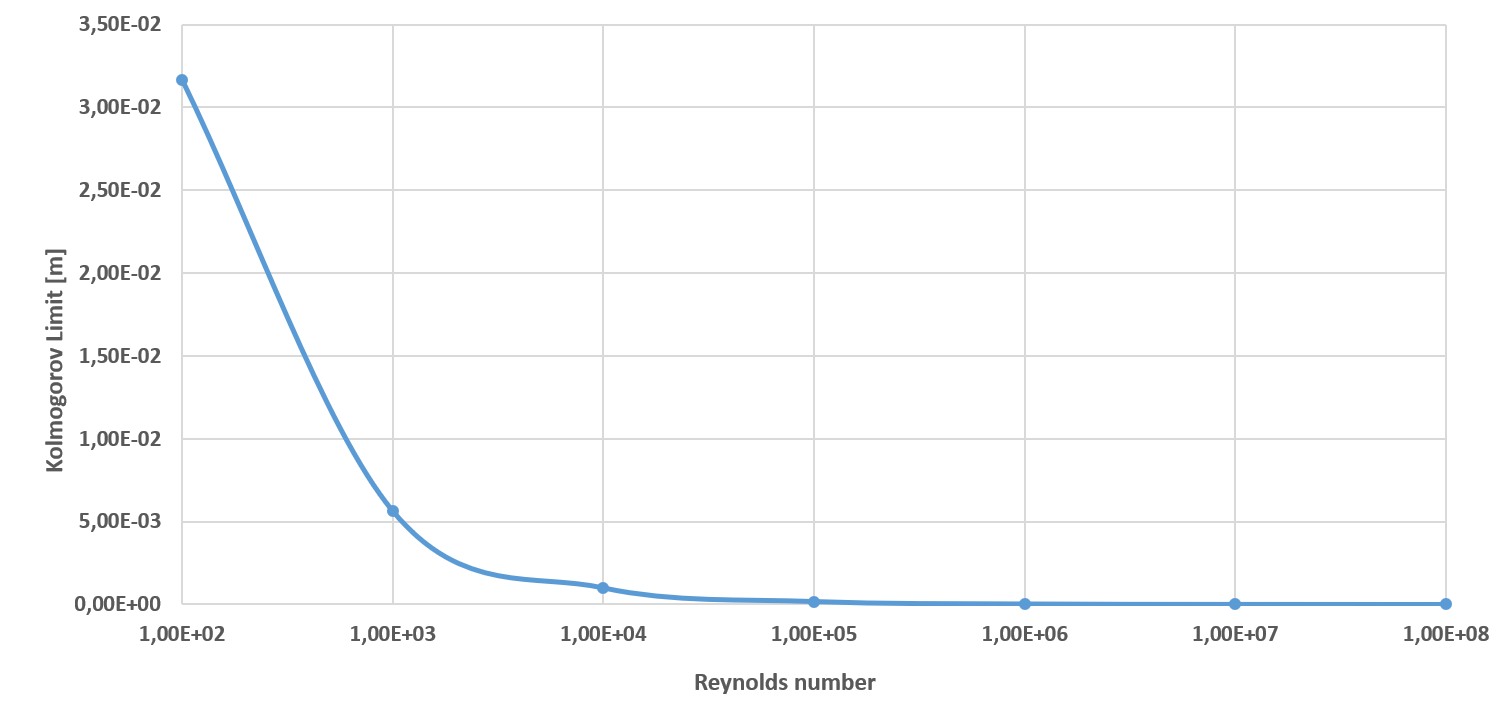
\includegraphics[width=0.85\textwidth]{Pictures/kolm_scale.png}
%\caption{Kolmogorov limit for given Reynolds number}
%\label{kolmscale}
%\end{figure}


\subsection{Large Eddy Simulation} \label{LES}
Large eddy simulation (LES) is a mathematical model for modeling turbulent flows used in computational fluid dynamics. It was initially proposed in 1963 by Joseph Smagorinsky to simulate atmospheric air currents \citep{LES1}.

The principal idea behind LES is to reduce the computational cost by ignoring the smallest length scales, which are the most computationally expensive to resolve, via low-pass filtering of the Navier–Stokes equations. Such a low-pass filtering, which can be viewed as a time- and spatial-averaging, effectively removes small-scale information from the numerical solution. This information is not irrelevant, however, and its effect on the flow field must be modeled, a task which is an active area of research for problems in which small-scales can play an important role, such as acoustics \citep{LES2}.

The governing equations employed for LES are obtained by filtering the time dependent Navier-Stokes equations in either Fourier (wave-number) space or configuration (physical) space. The filtering process effectively filters out the eddies whose scales are smaller than the filter width or grid spacing used in the computations. The resulting equations therefore governs the dynamics of large eddies \citep{fluenttheory}.

A filtered variable is defined by:
\begin{equation} \label{eq:lesfilter}
\overline{\phi}(x) = \int\displaylimits_{D} \phi \left( x' \right) G \left( x, x' \right) dx'
\end{equation}

\noindent where $D$ is the fluid domain, and $G$ is the filter function that determines the scale of the resolved eddies. The finite volume discretization itself implicitly provides the filtering operation:

\begin{equation} \label{eq:lesfilter2}
\overline{\phi}(x) = \frac{1}{V} \int\displaylimits_{\nu} \phi \left( x' \right) dx', \; x' \in \nu
\end{equation}

\noindent where $V$ is the volume of a computational cell. The filter function, $G(x, x')$ implied here is then:

\begin{equation} \label{eq:lesfilter3}
G(x, x') = 
\begin{cases}
	\frac{1}{V}, & \text{if } x'\in \nu \\
	0, & \text{otherwise}
\end{cases}
\end{equation}

For compressible flows, it is convenient to introduce the density-weighted (or Favre) filtering operator:
\begin{equation} \label{eq:favre}
\tilde{\phi} = \frac{\overline{\rho \phi}}{\overline{\phi}}
\end{equation}

Filtering the continuity \ref{eq:cont} and momentum \ref{eq:momentum} equations following form is obtained:

\begin{equation} \label{eq:lescont}
\frac{\partial \rho}{\partial t} + \frac{\partial}{\partial x_i} \left( \rho \overline{u_i} \right) = 0
\end{equation}

\begin{equation} \label{eq:lesmom}
\frac{\partial}{\partial t} \rho \overline{u_i}
+ \frac{\partial}{\partial x_j} \left( \rho \overline{u_i} \overline{u_j} \right)
= \frac{\partial}{\partial x_j} \left( \sigma_{ij} \right)
- \frac{\partial \overline{p}}{\partial x_i}
- \frac{\partial \tau_{ij}}{\partial x_j}
\end{equation}

\noindent where $\sigma_{ij}$ is the stress tensor due to molecular viscosity defined by:

\begin{equation} \label{eq:lesstress}
\sigma_{ij}
\equiv
\left[ \mu \left( \frac{\partial \overline{u_i}}{\partial x_{j}} + \frac{\partial \overline{u_j}}{\partial x_{i}} \right) \right]
- \frac{2}{3} \mu \frac{\partial \overline{u_l}}{\partial x_l} \delta_{ij}
\end{equation}

\noindent and $\tau_{ij}$ is the subgrid-scale stress defined by:

\begin{equation} \label{eq:lessubstress}
\tau_{ij} \equiv \rho \overline{u_i u_j} - \rho \overline{u_i} \; \overline{u_j}
\end{equation}

The Favre Filtered Navier-Stokes equation takes the same form as equation \ref{eq:lesmom}. The compressible form of the subgrid stress tensor is defined as:

\begin{equation} \label{eq:lescompsub}
\tau_{ij} = \overline{\rho} \tilde{u_i u_j} - \overline{\rho} \tilde{u_i} \; \tilde{u_j}
\end{equation}

The subgrid-scale stresses resulting from the filtering operation are unknown, and require modeling. The subgrid-scale turbulence models employ the Boussinesq hypothesis \citep{bousinesque} in the RANS models, computing subgrid-scale turbulent stresses from:

\begin{equation} \label{eq:lesturbstress}
\tau_{ij} - \frac{1}{3} \tau_{kk} \delta_{ij} = -2 \mu_{t} \overline{S_{ij}}
\end{equation}

\noindent where $\mu_t$ is the subgrid-scale turbulent viscosity. The isotropic part of the subgrid-scale stresses $\tau_{kk}$ is not modeled, but added to the filtered static pressure term. $S_{ij}$ is the rate-of-strain tensor for the resolved scale defined by:

\begin{equation} \label{eq:lesstrain}
\overline{S_{ij}} \equiv \frac{1}{2} \left( \frac{\partial \overline{u_i}}{\partial x_j} + \frac{\partial \overline{u_j}}{\partial x_i} \right)
\end{equation}

Equation \ref{eq:lescompsub} is split into its isotropic and deviatoric parts:

\begin{equation} \label{eq:lesdeviatoric}
\tau_{ij} - \frac{1}{3} \tau_{kk} \delta_{ij} = -2 \mu_{t} \left( S_{ij} - \frac{1}{3} S_{kk} \delta_{ij} \right)
\end{equation}

Using LES approach is viable for resolving directly formulated noise, yet the computational cost of such calculations is still relatively large due to mesh sizing requirements. As stated by \citep{LES_size} the required node count for the analysis can be described by formulas \ref{eq:leswm} and \ref{eq:leswr} for modeled and resolved boundary layers respectively.

\begin{equation} \label{eq:leswm}
N_{wm} = 54.7 \frac{L_z}{L_x} n_x n_y n_z Re^{2/7}_{L_x} \left[ \left( \frac{Re_{L_x}}{Re_{x_0}} \right)^{(5/7)} - 1\right]
\end{equation}

\begin{equation} \label{eq:leswr}
N_{wr} = 0.021 \frac{n_y}{\Delta x_w^{+} \Delta z_w^{+}} \frac{L_z}{L_x} Re^{13/7}_{L_x} \left[ 1 - \left( \frac{Re_{L_x}}{Re_{x_0}} \right)^{(6/7)} \right]
\end{equation}

The computational box for this case is of size $L_x \times \delta \times L_z$ in streamwise, normal to plate and spanwise direction respectively, where $\delta$ is the boundary layer thickness.

For $L_z / L_x = 4$ and $Re_{x_0} = 5 \cdot 10^5$ the node count for streamwise $Re = 10^6$ and $Re = 10^7$ is computed. The $n_x n_y n_z$ product is the number of grid points to resolve the cubic computational volume $\delta^3$ exterior to the viscous wall region. Suggested value of $n_x n_y n_z = 2500$, where $n_x = 10 \; n_y = 25 \; n_z = 10$ was used for the computation of node count with equation \ref{eq:leswm}. Suggested $\Delta x_w^{+} \approx 100$, $\Delta z_w^{+} \approx 20$ and $n_y \approx 10$ was used for computation of node count with equation \ref{eq:leswr}.

Node count for $Re = 10^6$ is roughly $1.82 \cdot 10^{7}$ nodes for modelled and $2.61 \cdot 10^{7}$ nodes for resolved wall flow. For $Re = 10^7$ the figures are $4.10 \cdot 10^{8}$ and $3.88 \cdot 10^{9}$ nodes respectively \citep{LES_size}.

It must be noted that provided cell count is solely for a flow box of boundary layer width. Respective mesh sizing should be propagated towards volume of the computational domain thus enlarging the mesh even further.

LES analyses are commonly used in research and engineering and the method used is feasible for the direct noise formulation. The computational expense of the LES analysis is high, although manageable. It must be noted, that at time of performing this study the resources to carry out the analysis of that king were unavailable to the author. Second limiting factor for LES is the amount of data generated during the process. As the direct approach requires storing at least every second time step for further processing, terabytes of data are predicted.

\subsection{Reynolds Averaged Navier Stokes} \label{RANS}
The most computationally efficient method for resolving turbulent flows is using Reynolsds Averaged Navier Stokes equation.

Consider a conservation variable $\phi$ of fluid described by spatial and temporal variables. The quantity may be decomposed to a sum of time averaged value in given spatial coordinates and time dependent fluctuations (eq. \ref{eq:rdecomp}).

%\begin{equation} \label{eq:NS}
%\rho \left(\frac{\partial u_i}{\partial t} + u_j \frac{\partial u_i}{x_j} \right) = - \frac{\partial p}{\partial x_j} + \mu \frac{\partial^2 u_i}{\partial x_j \partial x_j} + \frac{\mu}{3} \frac{\partial^2 u_j}{\partial x_i \partial x_j} + \rho g_i
%\end{equation}

\begin{equation} \label{eq:rdecomp}
\phi (x, y, z, t) = \overline{\phi (x, y, z, t)} + \phi ' (x, y, z, t)
\end{equation}

Consider at first the continuity equation \ref{eq:cont}. By applying Reynolds decomposition to velocity vector we obtain:

\begin{equation} \label{eq:cont_rans1}
\frac{\partial \rho}{\partial t} + \frac{\partial \overline{\rho u_i}}{\partial x_i} + \frac{\partial \rho u'_i}{\partial x_i} = 0
\end{equation}

By averaging the both sides of the equation  \ref{eq:cont_rans1} and applying averaging rules to its components we obtain:

\begin{equation} \label{eq:cont_rans2}
\frac{\partial \rho}{\partial t} + \frac{\partial \overline{\overline{\rho u_i}}}{\partial x_i} + \frac{\partial \overline{\rho u'_i}}{\partial x_i} = 0
\end{equation}

Because the average of an average is equal average, and  the average of the fluctuation component is equal 0 we obtain equation \ref{eq:cont_rans3}, the Reynolds averaged continuity equation.

\begin{equation} \label{eq:cont_rans3}
\frac{\partial \rho}{\partial t} + \frac{\partial \overline{\rho u_i}}{\partial x_i} = 0
\end{equation}

By taking the momentum equation \ref{eq:momentum}, switching to the index notation and applying the Reynolds decomposition we obtain the equation \ref{eq:mom_decomp1}

\begin{equation} \label{eq:mom_decomp1}
\underbrace{\frac{\partial \left( \overline{u_i} + u'_i \right)}{\partial t}}_\text{1} 
+ \underbrace{\left( \overline{u_j} + u'_j \right) \frac{\partial \left( \overline{u_j} + u'_j \right)}{\partial x_j}}_\text{2} 
=
- \underbrace{\frac{1}{\rho} \frac{\partial \left( \overline{p} + p' \right)}{\partial x_i}}_\text{3} 
+ \underbrace{\nu \frac{\partial^2 \left( \overline{u_i} + u'_i \right)}{\partial x_j^2}}_\text{4} 
\end{equation}

Components 1, 3 and 4 of the above equation are treated in the same manner as the continuity equation and thus we obtain:

\begin{equation} \label{eq:mom_components}
\underbrace{\frac{\partial \overline{u_i}}{\partial t}}_\text{1}
\qquad
\underbrace{\frac{1}{\rho} \frac{\partial \overline{p}}{\partial x_i}}_\text{3}
\qquad
\underbrace{\nu \frac{\partial^2 \overline{u_i}}{\partial x_j^2}}_\text{4}
\end{equation}

The decomposition of component 2 from the equation \ref{eq:mom_decomp1} requires multiplication of the components within the braces and performing Reynolds averaging on each of the products: 

\begin{equation} \label{eq:mom_comp2_avg}
\underbrace{\overline {\left( \left( \overline{u_j} + u'_j \right) \cdot \frac{\partial \left( \overline{u_i} + u'_i \right)}{\partial x_j} \right)}}_\text{2}
= \underbrace{\overline{\left( \overline{u_j} \frac{\partial \overline{u_i}}{\partial x_j} \right)}}_\text{M $\cdot$ M $\neq$ 0}
+ \underbrace{\overline{\left( \overline{u_j} \frac{\partial u'_i}{\partial x_j} \right)}}_\text{M $\cdot$ F = 0}
+ \underbrace{\overline{\left( u'_j \frac{\partial \overline{u_i}}{\partial x_j} \right)}}_\text{F $\cdot$ M = 0}
+ \underbrace{\overline{\left( u'_j \frac{\partial u'_i}{\partial x_j} \right)}}_\text{F $\cdot$ F $\neq$ 0}
\end{equation}

The F $\cdot$ F $\neq$ 0 product can be further simplified by equation:

\begin{equation} \label{eq:ff}
\frac{\partial u'_j u'_i}{\partial x_j}
= \underbrace{u'_i \frac{\partial u'_j}{\partial x_j}}_\text{= 0}
+ \underbrace{u'_j \frac{\partial u'_i}{\partial x_j}}_\text{F $\cdot$ F $\neq$ 0}
\end{equation}

By inserting the components 1 through 4 from equations \ref{eq:mom_components} and \ref{eq:mom_comp2_avg} modified by equation \ref{eq:ff} to the equation \ref{eq:mom_decomp1} we obtain the Reynolds averaged momentum equation:

\begin{equation} \label{eq:RANSmomentum}
\frac{d \overline{U}}{dt}
=
- \frac{1}{\rho} \frac{\partial \overline{p}}{\partial x_i}
+ \frac{\partial}{\partial x_j} \left[ \nu \frac{\partial \overline{u_j}}{\partial x_j} - \overline{u'_i u'_j}\right]
\end{equation}

By representing the viscous terms as a stress tensor (eq. \ref{eq:viscous}) we obtain the momentum equation with turbulent stress (eq \ref{eq:RANSmomentum2})

\begin{equation} \label{eq:viscous}
\nu \frac{\partial^2 \overline{u_i}}{\partial x_j^2}
=
\frac{1}{\rho} \frac{\partial}{\partial x_j} \tau_{ij}
\end{equation}

\begin{equation} \label{eq:RANSmomentum2}
\frac{d \overline{U}}{dt}
=
- \frac{1}{\rho} \nabla \overline{p}
+ \frac{1}{\rho} \frac{\partial}{\partial x_j} \left[ \tau_{ij} - \rho \overline{u'_i u'_j} \right]
\end{equation}

The $\rho \overline{u'_i u'_j}$ term can be further transformed to Reynolds stress tensor linked to shear stress.

The remaining fluctuating component is then modeled rather than resolved, by one of many turbulence model based on Bousinessque theory.

\subsection{Hybrid RANS/LES Methods}
At first, the concepts of Reynolds Averaging and Spatial Filtering seem incompatible, as they result in different additional terms in the momentum equations (Reynolds Stresses and sub-grid stresses). This would preclude hybrid models like Scale-Adaptive Simulation (SAS), Detached Eddy Simulation (DES), Shielded DES (SDES), or Stress-Blended Eddy Simulation (SBES), which are based on one set of momentum equations throughout the RANS and LES portions of the domain. However, it is important to note that once a turbulence model is introduced into the momentum equations, they no longer carry any information concerning their derivation (averaging). Case in point is that the most popular models, both in RANS and LES, are eddy viscosity models that are used to substitute either the Reynolds- or the sub-grid stress tensor. After the introduction of an eddy viscosity (turbulent viscosity), both the RANS and LES momentum equations are formally identical. The difference lies exclusively in the size of the eddy-viscosity provided by the underlying turbulence model. This allows the formulation of turbulence models that can switch from RANS to LES mode, by lowering the eddy viscosity in the LES zone appropriately, without any formal change to the momentum equations \citep{fluenttheory}.

For further calculations, Delayed Detached Eddy Simulation with $k-\omega \, SST$ model was chosen. In the DES approach, the unsteady RANS models are employed in the boundary layer, while the LES treatment is applied to the separated regions. The LES region is normally associated with the core turbulent region where large unsteady turbulence scales play a dominant role. In this region, the DES models recover LES-like subgrid models. In the near-wall region, the respective RANS models are recovered \citep{fluenttheory}.

Formulation of DES is the development of the Spalart-Allmaras turbulence model for RANS formulation \citep{desspalart}, therefore the theoretical formulations are derived from the S-A model.

The S-A model uses modified turbulent viscosity $\tilde{\nu}$ in place of the turbulent kinematic viscosity.

\begin{equation} \label{eq:nutilde}
\frac{\partial}{\partial t} \left( \rho \tilde{\nu} \right)
+ \frac{\partial}{\partial x_i} \left( \rho \tilde{\nu} u_i \right)
= G_{\nu} + \frac{1}{\sigma_{\tilde{\nu}}}
\left[
\frac{\partial}{\partial t} \left\lbrace \left( \mu + \rho \tilde{\nu} \right) \frac{\partial \tilde{\nu}}{\partial x_j} \right\rbrace
+ C_{b2} \rho \left( \frac{\partial \tilde{\nu}}{\partial x_{j}}\right)^{2}
\right]
- Y_{\nu} + S_{\tilde{\nu}}
\end{equation}

Turbulence production $G_{\nu}$ and destruction $Y_{\nu}$ terms are modeled as:

\begin{equation} \label{eq:SAGnu}
G_{\nu} = C_{b1} \rho \tilde{S} \tilde{\nu}
\end{equation}

\begin{equation} \label{eq:SAYnu}
Y_{\nu} = C_{wq} \rho f_{w} \left(\frac{\tilde{\nu}}{d} \right)^2
\end{equation}

\noindent where $d$ is the length scale calculated as the distance to the closest wall and $\tilde{S}$ being the measure of deformation tensor:

\begin{equation} \label{eq:SAdeform}
\tilde{S} \equiv S + \frac{\tilde{\nu}}{\kappa^2 d^2} f_{v2}
\end{equation}

\noindent where:

\begin{equation} \label{eq:SAdeform2}
S \equiv \lvert \Omega_{ij} \rvert + C_{prod} \text{min} \left(0, \lvert S_{ij} \rvert - \lvert \Omega_{ij} \rvert \right)
\end{equation}

\noindent where:

\begin{equation} \label{eq:SAdeform3}
C_{prod} = 2.0, \;
\lvert \Omega_{ij} \rvert \equiv \sqrt{2 \Omega_{ij} \Omega_{ij}}, \;
\lvert S_{ij} \rvert \equiv \sqrt{2 S_{ij} S_{ij}}
\end{equation}

\noindent with the mean strain rate defined as:

\begin{equation} \label{eq:SAdeform4}
S_{ij} = \frac{1}{2} \left( \frac{\partial u_j}{\partial x_i} + \frac{\partial u_i}{\partial u_j}\right)
\end{equation}

The equation \ref{eq:SAYnu} shows that $\tilde{\nu}$ is proportional to the local deformation rate and wall distance: $\tilde{\nu} \propto Sd^2$. Smagorinsky model for "Sub-Grid-Scale" (SGS) scales the turbulent viscosity with local deformation and grid spacing: $\tilde{\nu} \propto S \Delta^2$.

By replacing the $d$ in the S-A destruction term (eq. \ref{eq:SAYnu}) with $\tilde{d}$:
\begin{equation} \label{eq:tilded}
\tilde{d} \equiv \text{min} \left(d, C_{DES} \Delta \right)
\end{equation}

\noindent a single model is obtained, acting as RANS with S-A turbulence modeling in regions where $d \ll \Delta$ and with LES behavior where $d \gg \Delta$. Grid spacing $\Delta$ is defined as the largest dimension of the computational cell $\Delta \equiv \text{max}\left( \Delta x, \Delta y, \Delta z\right)$.  In case of an ambiguous grid definition, where $\Delta < \delta$ the DES limiter can activate the LES mode inside the boundary layer, where the grid is not fine enough to sustain resolved turbulence. Therefore, a new formulation \citep{ddesspalart} of DES is available to preserve the RANS mode throughout the boundary layer. This is known as the delayed option or DDES for delayed DES \citep{fluenttheory}.

DES and DDES methods can be used with other RANS turbulence models. Further analyses presented in this thesis use a $k-\omega \, SST$ model. For hybrid model the dissipation of turbulent kinetic energy is modified:

\begin{equation} \label{eq:deskoYk}
Y_k = \rho \beta^{*} k \omega F_{DES}
\end{equation}

\noindent where:

\begin{equation} \label{eq:deskoFdes}
F_{DES} = \text{max}\left( \frac{L_t}{C_{DES} \Delta_{max}}\left( 1-F_{SST} \right), 1 \right)
\end{equation}

\noindent where $C_{DES}$ is a calibration constant used in the DES model and has a value of 0.61, with $F_{SST} = 0, F_1, F_2$ where $F_1$ and $F_2$ are the blending functions of  the Baseline and $k-\omega \, SST$ model. The turbulent length scale is the parameter that defines this RANS model:

\begin{equation} \label{eq:deskoFdes2}
F_{DES} = \text{max}\left( \frac{L_t}{C_{DES} \Delta_{max}}, 1 \right)
\end{equation}

The $F_{DDES}$ blending function is given by equation \ref{eq:deskoFdes2} with model constants \mbox{$C_{d1} = 20$}, \mbox{$C_{d2} = 3$} and $r_d$ as defined by eq. \ref{eq:deskord}:

\begin{equation} \label{eq:deskoFddes}
F_{DDES} = \tanh \left[ \left( C_{d1} r_{d1} \right)^{C_{d2}} \right]
\end{equation}

\begin{equation} \label{eq:deskord}
r_d = \frac{\nu_t + \nu}{\kappa^2 y^2 \sqrt{0.5 \left( S^2 + \Omega^2 \right)}}
\end{equation}

%-----------------------------------
%	SECTION
%-----------------------------------
\section{Mesh sizing requirements} \label{meshsize}
Let's assume a sinusoidal pressure fluctuation $y(t)$ (eq. \ref{eq:sine}) of ordinary frequency of $f$ and amplitude $A$, moving through ambient medium for more than 5 cycles at speed of sound (eq. \ref{eq:sos}). The mathematical and numerical methods for solving flow field described in section above are capable of computing such pressure fluctuation in a computational mesh of relevant resolution. 

\begin{equation} \label{eq:sine}
y(t) = A \sin(2 \pi f t + \phi)
\end{equation}

\begin{equation} \label{eq:sos}
a = \sqrt{\kappa R T}
\end{equation}

Cell size and time step size are limited by the wave length, and therefore frequency of the discussed pressure fluctuation. The wavelength is calculated by formula \ref{eq:wl}.

\begin{equation} \label{eq:wl}
\lambda = \frac{v}{f}
\end{equation}

Considered fluctuation travels through the finite volumes (that is: CFD mesh cells) in the stationary CFD mesh. Pressure value is measured at the cell centroid for each timestep. At this stage, it is assumed that timestep is of relevant resolution for the analysis, the mesh is isotropic in $x$, $y$ and $z$ directions and that the propagation has only one directional component. Four possibilities are considered.

%\begin{itemize}
\textbf{Scenario 1:} wavelength is smaller than the edge length of the cell in the direction of propagation. In this condition, the pressure fluctuation performs a number of cycles within one cell (Fig. \ref{scen1}). Due to the numerical approach, such fluctuation will be filtered out.

\begin{figure}[h!]
\centering % bo \centering nie wstawia dodatkowego odstępu

\includegraphics[width=0.5\textwidth]{Pictures/placeholder.jpg}
\caption{Scenario 1. Wavelength smaller than cell edge length}
\label{scen1}
\end{figure}

\textbf{Scenario 2:} wavelength and cell edge length in the direction of propagation are equal. In this condition, the pressure fluctuation performs one cycle within one cell in the direction of the fluctuation propagation (Fig. \ref{scen2}). Such pressure change will be also filtered out by the numerical scheme.

\begin{figure}[h!]
\centering % bo \centering nie wstawia dodatkowego odstępu

\includegraphics[width=0.5\textwidth]{Pictures/placeholder.jpg}
\caption{Scenario 2. Wavelength equal to cell edge length}
\label{scen2}
\end{figure}

\textbf{Scenario 3:} wavelength is equal to 4 cell edge lengths. This is the minimum cell size condition for proposed approach. In this condition, the pressure fluctuation performs one cycle within four cells in the direction of the fluctuation propagation (Fig. \ref{scen3}). FVM method is now capable of computing the pressure fluctuations resulting from sound wave propagation.

\begin{figure}[h!]
\centering % bo \centering nie wstawia dodatkowego odstępu

\includegraphics[width=0.5\textwidth]{Pictures/placeholder.jpg}
\caption{Scenario 3. Wavelength equal four minimum edge lengths}
\label{scen3}
\end{figure}

\textbf{Scenario 4:} wavelength is larger than 4 cell edge lengths. In this condition, the pressure fluctuation performs one cycle within multiple cells in the direction of the fluctuation propagation (Fig. \ref{scen4}). FVM method computes pressure from the sound wave propagation across multiple cells.

\begin{figure}[h!]
\centering % bo \centering nie wstawia dodatkowego odstępu

\includegraphics[width=0.5\textwidth]{Pictures/placeholder.jpg}
\caption{Scenario 4. Wavelength larger than four minimum edge lengths}
\label{scen4}
\end{figure}
%\end{itemize}

Based on these possibilities, the edge sizing of the finite volume cell should be at least four times smaller than the shortest wavelength expected in the flowfield.

%----------------------------------------------------------------------------------------
%	SECTION
%----------------------------------------------------------------------------------------
\section{Timestep requirements} \label{timestepsize}
There are two limiting factors for timestep requirements. The high frequency signal is limited by the timestep size, whereas the low frequencies are limited to the total number of timesteps and physical flow time calculated. The timestep size is calculated first.

Once mesh cell sizing is established, time at which the fluctuation passes the cell is established by simple formula \ref{eq:vel2}. Distance $s$ is the cell edge sizing, obtained as in section \ref{meshsize} and the relation between cell size and wavelength is presented in equation \ref{eq:dist}.

\begin{equation} \label{eq:vel2}
a = \frac{s}{t}
\end{equation}

\noindent where

\begin{equation} \label{eq:time}
t = \frac{1}{f}
\end{equation}

\begin{equation} \label{eq:dist}
s = \frac{\lambda}{4}
\end{equation}

By rearranging the equation \ref{eq:vel2} to solve for $t$ and substituting $\lambda$ by \ref{eq:wl} we obtain:

\begin{equation} \label{eq:mintime}
t = \frac{s}{a} = \frac{\lambda}{4a} = \frac{a}{f} \cdot \frac{1}{4a} = \frac{1}{4f}
\end{equation}

Time step $t$ must comply with the requirements of the FFT analysis occurring further in the process as it becomes the minimum sampling time for the sound pressure signal. Therefore it must be compared with the requirements stated by Shannon-Nyquist-Whitaker theorem: \textit{If a function x(t) contains no frequencies higher than B hertz, it is completely determined by giving its ordinates at a series of points spaced 1/(2B) seconds apart.}

Equation \ref{eq:mintime} shows that time step for the analysis is dependent from the expected value of high frequency fluctuations. %Four scenarios can be discussed.

%\textbf{Scenario 1:} timestep is smaller than 1/4 of the fluctuation period (Fig. \ref{time1}).

%\begin{figure}[h!]
%\centering % bo \centering nie wstawia dodatkowego odstępu
%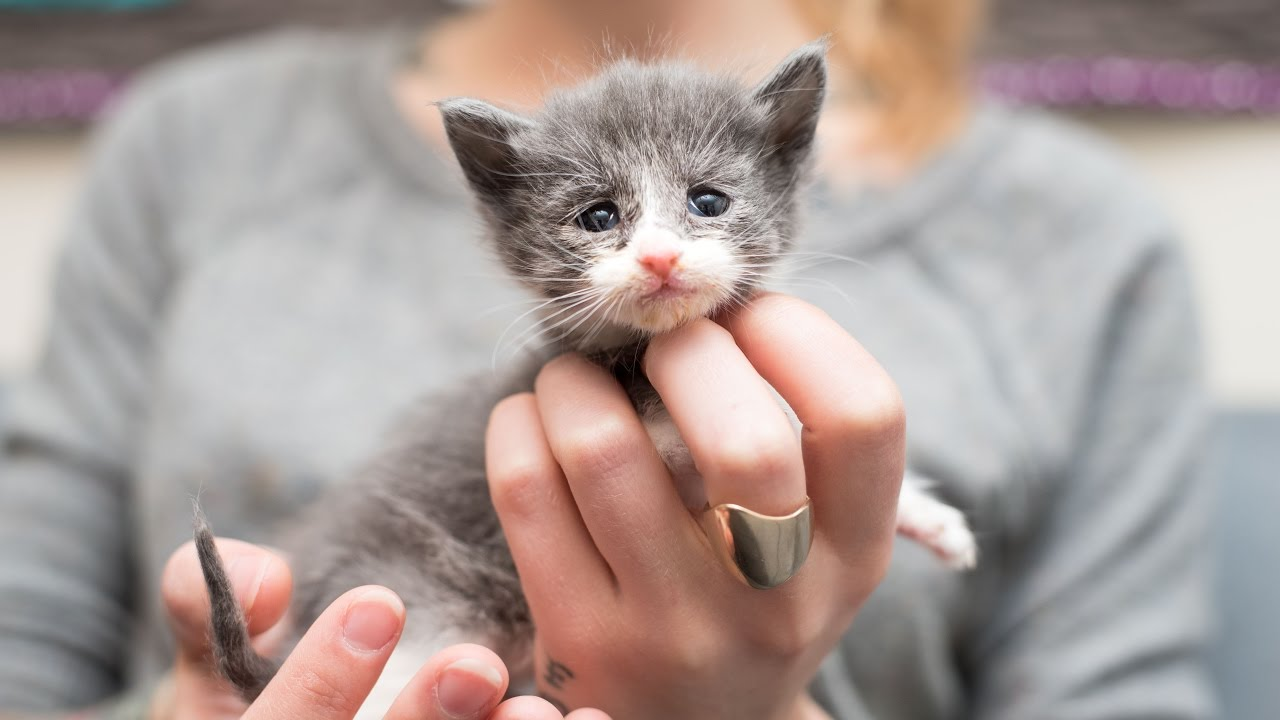
\includegraphics[width=0.5\textwidth]{Pictures/kitten-placeholder.jpg}
%\caption{Scenario 1. Timestep smaller than 1/4 of fluctuation period}
%\label{time1}
%\end{figure}

%\textbf{Scenario 2:} timestep is equal to the  1/4 of the fluctuation period (Fig. \ref{time2}).

%\begin{figure}[h!]
%\centering % bo \centering nie wstawia dodatkowego odstępu
%%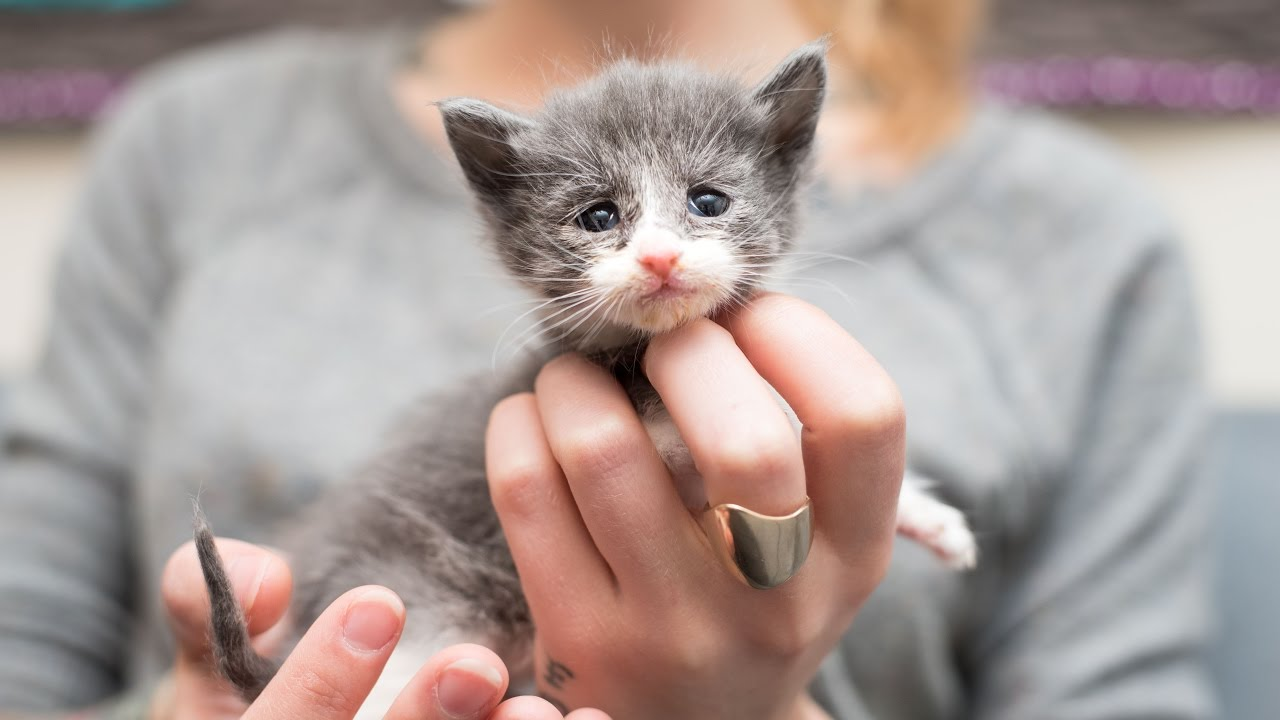
\includegraphics[width=0.5\textwidth]{Pictures/kitten-placeholder.jpg}
%\caption{Scenario 2. Timestep equal to 1/4 of fluctuation period}
%\label{time2}
%\end{figure}

%\textbf{Scenario 3:} timestep is equal to fluctuation period (Fig. \ref{time3}).

%\begin{figure}[h!]
%\centering % bo \centering nie wstawia dodatkowego odstępu
%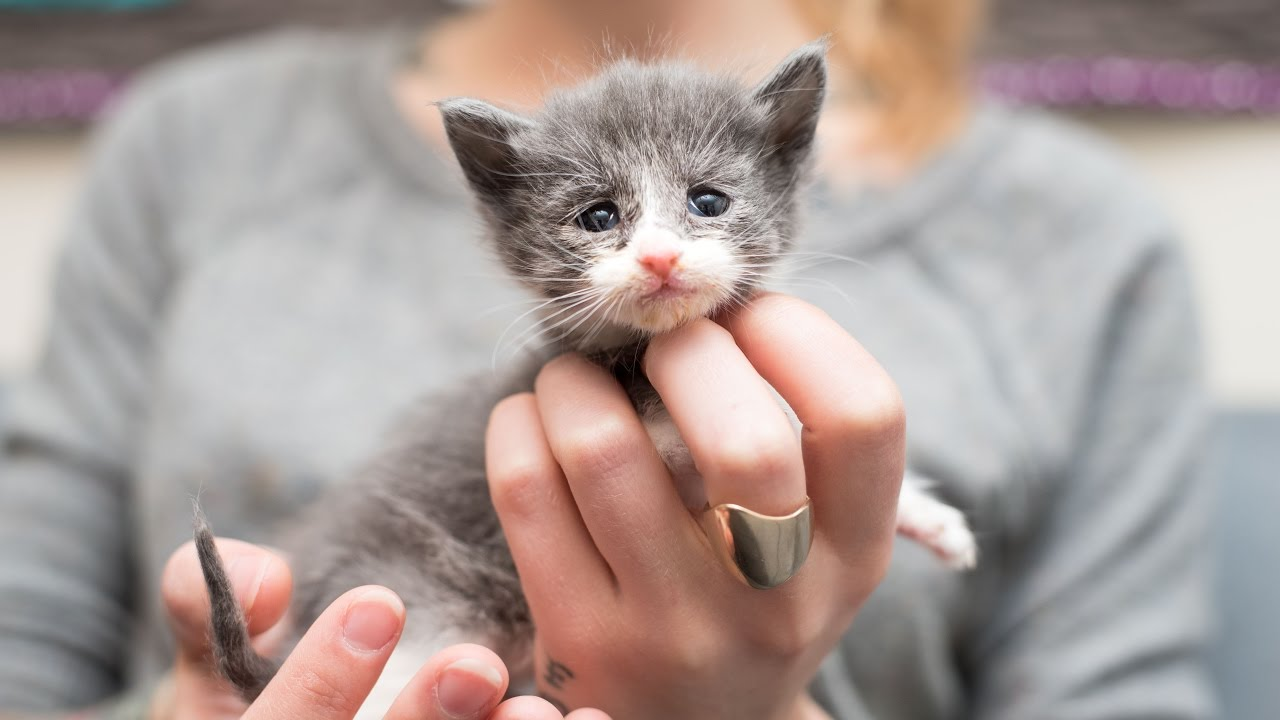
\includegraphics[width=0.5\textwidth]{Pictures/kitten-placeholder.jpg}
%\caption{Scenario 3. Timestep equal to fluctuation period}
%\label{time3}
%\end{figure}

%\textbf{Scenario 4:} timestep is larger that fluctuation period (Fig. \ref{time4}).

%\begin{figure}[h!]
%\centering % bo \centering nie wstawia dodatkowego odstępu
%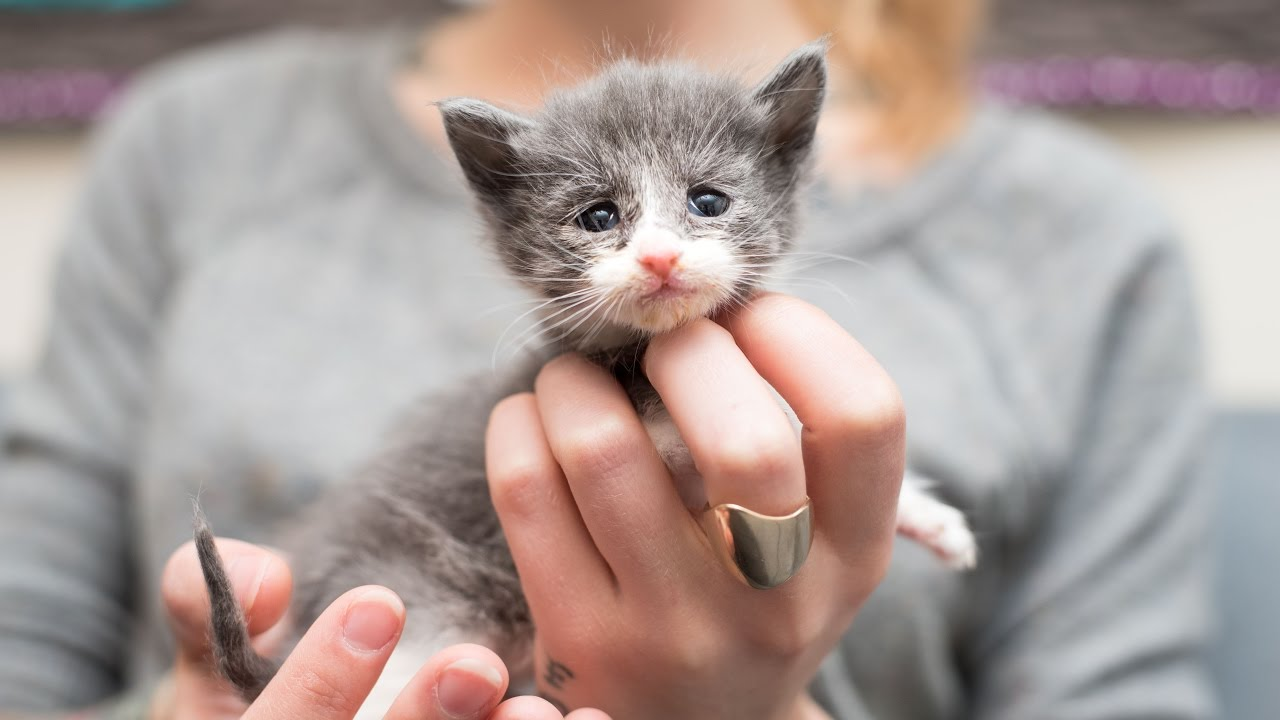
\includegraphics[width=0.5\textwidth]{Pictures/kitten-placeholder.jpg}
%\caption{Scenario 4. Timestep is larger than fluctuation period}
%\label{time4}
%\end{figure}
%\end{itemize}

In order to capture frequencies on the low end of the spectrum, the analysis must be performed long enough to capture at least a single, with optimum 5 or more fluctuations of the desired low frequency. Assuming lower end of the audible frequency spectrum, the 20Hz frequency, the simulation time must resemble at least 0.05s of flowtime with optimum 0.25s of flowtime at given timestep.


%----------------------------------------------------------------------------------------
%	SECTION
%----------------------------------------------------------------------------------------
\section{Limiting factors of the direct approach} \label{limits}
Described direct formulation noise analysis is solely a post processing approach relying on data generated on CFD analysis. In order to obtain reasonable results down the process, the analysis itself mus be capable of delivering pressure fluctuations that can be considered as acoustic in source. 

It is advised to used a turbulence model that is capable of resolving small scale turbulence on a mesh that will allow such resolution. Utilizing LES formulation or at least hybrid RANS/LES turbulence model such as DDES. Using an averaging formulation such as RANS will cut off all of the fluctuations and is not suitable for this approach.

%Pressure signal used by this approach is given by a list of real scalar values for each node or cell centroid for each timestep. Therefore obtaining phase shift of the ordinary sinuses components of pressure signal may be challenging, if at all possible, and relies solely on further postprocessing of generated data. 

The range of frequencies captured by this method depends on the mesh sizing and timestep sizing. Therefore, if the range of expected frequencies is known or at least estimated, the mesh sizing and timestep size can be adjusted for the given case. For analysis within audible range, 4000 timesteps are required for one 20Hz period. Considering the mesh sizing requirements, the mesh cell count will rise up to tens of millions for a single passage axial compressor blade. This makes the case files and storing data for each timestep relatively challenging and requires securing adequate storage beforehand.
 
A major limiting factor is the implementation of the direct noise formulation post-processing. For this thesis, the method was implemented in python v.3.5 high level programming language. Python code is written in C/C++ and provides a vast array of additional libraries for handling files, tabular data and performing mathematical operations. The code is presented in appendices to this dissertation. Although easy to implement, python code is known to be inefficient and slow while managing large amounts of data. Tools and algorithms used in implementing the averaging, obtaining sound pressure and particle velocity as well as DFT are build in tools from specific libraries. As convenient for the implementation, the post-processing code requires some amount of operational memory and disk space for generating the results.

The programming language used for the post-processing of data must be capable of generating 2D and 3D plots for visualization purposes. Ideally the processed and visualized data should resemble the mesh from which the initial data was gathered.

% Chapter Template

\chapter{Test case} % Main chapter title

\label{case} % Change X to a consecutive number; for referencing this chapter elsewhere, use \ref{ChapterX}

\lhead{\emph{Test case}} % Change X to a consecutive number; this is for the header on each page - perhaps a shortened title

%----------------------------------------------------------------------------------------
%	SECTION 1
%----------------------------------------------------------------------------------------
\section{NASA Rotor 67 transonic axial compressor}

The direct approach noise analysis is onducted on a NASA Rotor 67 (R67) transonic axial compressor. Originating as a first stage of two stage fan for evaluation of design procedures, validation of experimental facilities as well as meshing and CFD tools. The test case was used in a multitude of studies for turbomachinery aerodynamics, geometry optimisation, noise analyses and structural analyses. Full design procedure can be found in references \cite{r67design} and \citep{r67performance}. The CFD analysis and direct approach noise analysis is performed on a single passage of a first stage rotor of the compressor. The setup for the  calculations (apart from the single passage constraint) is relevant do case described in study \citep{r67laser}, which was the main source for geometry and flowfield data.

\begin{figure}[h!]
\centering % bo \centering nie wstawia dodatkowego odstępu
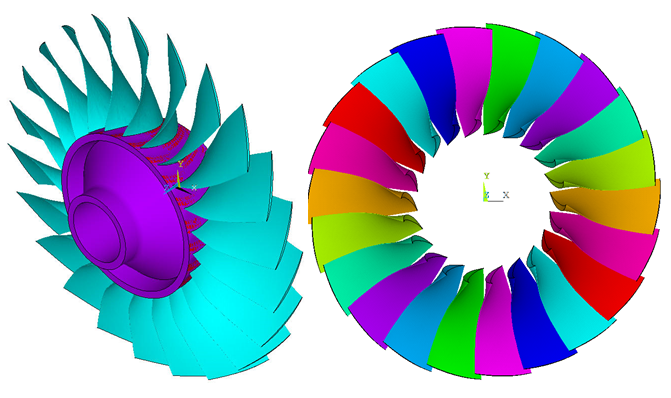
\includegraphics[width=0.85\textwidth]{Pictures/r67_over.png}
\caption{Geometry of NASA R67}
\label{r67over}
\end{figure}

Basic parameters of the given rotor are, design pressure ratio of 1.63 at massflow of 33.25 kg/sec. The design rotational speed is 16 043 rpm, which yields a tip speed of 429 m/s and an inlet tip relative Mach number of 1.38. The rotor has 22 blades and an aspect ratio of 1.56 (based on average span/root axial chord). The inlet and exit tip diameters are 514 and 485 mm, respectively, and the inlet and exit hub/tip radius ratios are 0.375 and 0.478, respectively. A fillet radius of 1.78 mm is used at the airfoil-hub juncture. The square root of the mean square of the airfoil surface finish is 0.8 $\mu${}m or better, the airfoil surface tolerance is $\pm$ 0.04 mm, and the running tip clearance is approximately 1.0 mm \citep{r67laser}. Surface roughness and some of the geometrical features are omitted during the preparation of the geometry and CFD mesh for reasons described in sections \ref{3dgeom} and \ref{mesh}. General geometry of NASA R67 is presented on fig \ref{r67over}. Basic parameters of the test subject are presented in table \ref{tab:data}

\begin{table}[ht!]
\centering
\caption{Basic R67 parameters} \label{tab:data}
\begin{tabular}{@{}lrr@{}}
\toprule
Parameter   & Value & Unit \\ \midrule
$\Pi$          & 1.63  & -    \\
$\dot{m}$      & 33.25 & kg/s \\
$\omega$       & 16043 & rpm  \\
$v_t$          & 429   & m/s  \\
$Ma_t$         & 1.38  & -    \\
blade count    & 22    & -    \\ \bottomrule
\end{tabular}
\end{table}

%----------------------------------------------------------------------------------------
%	SECTION
%----------------------------------------------------------------------------------------
\section{3D geometry preparation} \label{3dgeom}
%Geometry was prepared in Ansys ICEM 14.5 meshing software. Creating the geometry directly in the meshing software reduces the risk of creating flaws in the geometry, due to file translations. Mesh is created in millimeters.

References \citep{r67design} and \citep{r67performance} provide the blade geometry for both stages of the compressor as a Multiple-Circular-Arc definition. In the MCA approach the design blade elements lie on conical surfaces which approximate the actual stream flow surfaces. More specifically, the mean camber line and the suction and pressure surface lines of a blade element are lines with a constant rate of angle change with path distance on a specified conical surface \citep{bladecompose}. Although relatively comfortable for design purposes, such approach requires transforming the MCA blade to Cartesian or cylindrical coordinates. Reference \citep{bladecompose} provides an extended definition of MCA blade description as well as Fortran code for generating blade cross-section and computing geometric properties of the blade.

Source \citep{r67laser} provides a list of coordinates for 14 profiles of the 1st stage rotor blade suction and pressure surface, as well as coordinates for hub and casing path in the meridional plane. These coordinates were used to create the geometry of the single passage of the subject blade. Cartesian coordinates are also available in Appendix \ref{r67_coords_data} and project Github repository \citep{github}.

%Geometry alignment is presented on figure \ref{geom_gcs}.
The coordinate system is a standard right-hand Cartesian CS. Rotation axis is set to Z-axis with flow in positive Z direction. The compressor rotation is set as in right-hand rule, the compressor rotates in clockwise direction when viewing the blade leading edge. $Z = 0$ coordinate is defined by point number 1 on 1st blade design surface.

%\begin{figure}[h!]
%\centering % bo \centering nie wstawia dodatkowego odstępu
%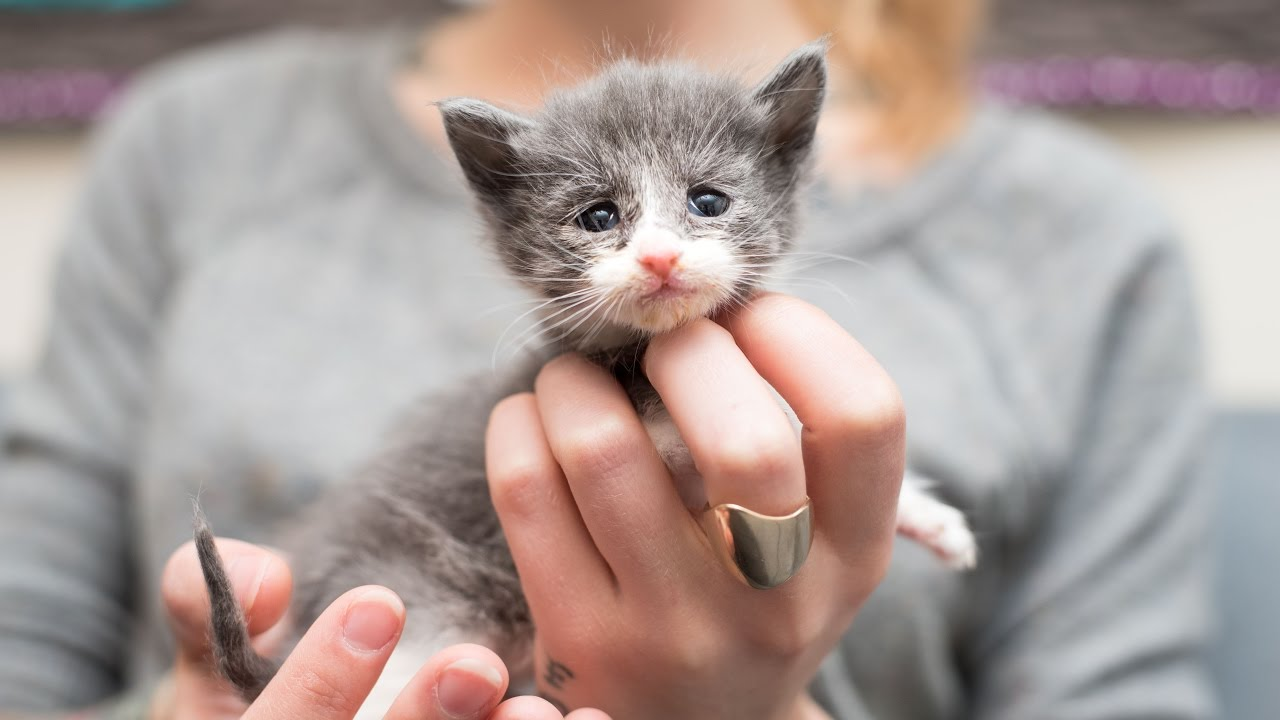
\includegraphics[width=0.85\textwidth]{Pictures/kitten-placeholder.jpg}
%\caption{Global coordinate system for geometry}
%\label{geom_gcs}
%\end{figure}

Hub and casing flow paths were created by importing formatted point data as a \mbox{b-spline} curve, followed by extrusion the curve to surface by rotating it by $\pm 60 \degree$. Suction and pressure surface of the blade were created by importing the Cartesian coordinates if the design airfoils and creating a lofted surface along the imported splines. Leading and trailing edge radii were created in a similar manner, with use of edge radius and edge tangency points given in original study \citep{r67laser}. Tip gap of the blade was created by offsetting the casing surface by 1.016 mm in the normal direction towards the rotation axis and creating a section line between blade surfaces and the offset surface.

Due to the estimated mesh cell count, only one blade passage is created, therefore~a set of periodic surfaces must be defined. ICEM software is capable of creating a midline as an average of coordinates of two given lines. A midline was created for every design profile and was manually extended beyond the blade leading and trailing edge. Midlines were lofted to create a midsurface which was later on copied with rotation by $\pm 0.5 \cdot \frac{360 \degree}{22}$ to create two identical periodic surfaces.

Aforementioned midlines were also rotated along Z-axis to create control surfaces for mesh stabilization and data acquisition down the process.

Reference \citep{r67laser} provides coordinates of hub and casing for the full experiment, however only a rotating part of the experimental rotor setup is be used. Two surfaces normal to Z direction at coordinates Z = -13.74 mm and Z = 93.65 mm are placed as inlet and outlet boundary conditions. Geometry was finished by necessary extrusions, trimming and other finishing operations to ensure high quality surface for meshing.

Physical experiment test compressor has a 1.78 mm fillet at airfoil-hub juncture. This feature was omitted as it would unnecessarily complicate the meshing process and increase the cell count.

Such approach allowed for creating a geometry for single blade passage with centered blade of 1st stage rotor of the test compressor (Fig \ref{geom_final}).

\begin{figure}[ht!]
\centering % bo \centering nie wstawia dodatkowego odstępu
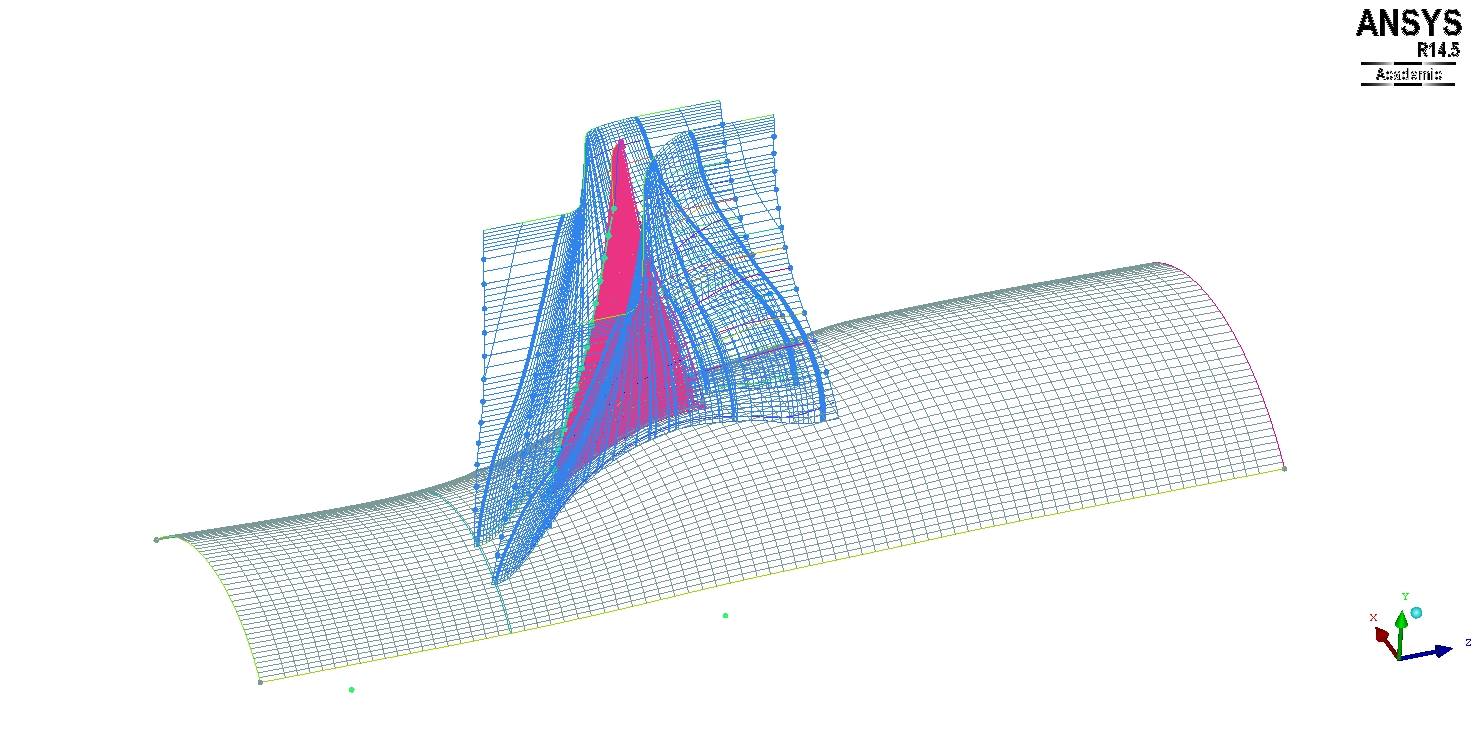
\includegraphics[width=0.85\textwidth]{Pictures/r67_geom.jpg}
\caption{Final single passage geometry. Some features hidden for clarity}
\label{geom_final}
\end{figure}

%----------------------------------------------------------------------------------------
%	SECTION
%----------------------------------------------------------------------------------------
\section{Meshing approach} \label{mesh}
Following requirements are posed to the mesh for the discussed case:
\begin{itemize}
\item[-]Possibly low number of elements fulfilling the mesh sizing requirements stated in chapter \ref{direct_approach},
\item[-] Mesh should be a fully structural mesh including the tip gap,
\item[-] The periodic boundary mesh must be identical/conforming for both boundaries,
\item[-] The mesh must have high quality metrics in terms of cell orthogonality and skew.
%\item The cell aspect ratio should be limited to 5000 as defined by equation \ref{eq:aspect} 
\end{itemize}

The orthogonal quality (or orhogonality) of the mesh is calculated as in equation \ref{eq:ortho}. The orthogonality value ranges from -1 to 1, where 1 denotes the best orthogonality, 0 -- a zero volume cell and -1 -- a cell with reversed normal direction or negative volume.

\begin{equation} \label{eq:ortho}
\text{Orthogonality} = \frac{\vec{A_i} \cdot \vec{f_i}}{|\vec{A_i}| \cdot |\vec{f_i}|}
\end{equation}

Schematic representation of vectors used for calculation of orthogonality are presented in figure \ref{ortho}.

\begin{figure}[ht!]
\centering % bo \centering nie wstawia dodatkowego odstępu
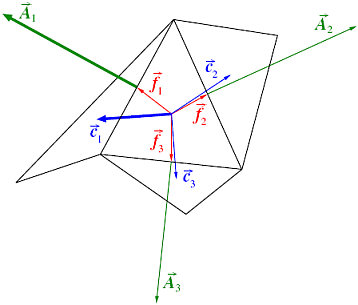
\includegraphics[width=0.85\textwidth]{Pictures/Quality_Orthogonal_cell.png}
\caption{Vectors Used to Compute Orthogonal Quality for a Cell}
\label{ortho}
\end{figure}

For a hexahedral element, skewness is defined as the normalized worst angle between each of the 6 face normals and the vector defined by the centroid of the hexahedron and the center of the face.

\begin{figure}[ht!]
\centering % bo \centering nie wstawia dodatkowego odstępu
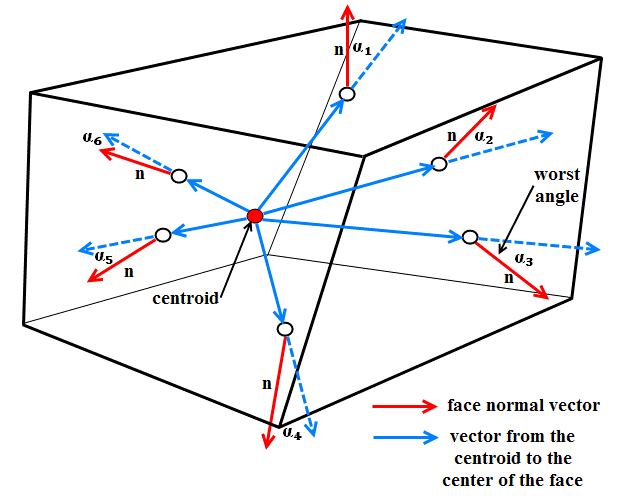
\includegraphics[width=0.85\textwidth]{Pictures/skew.png}
\caption{Vectors Used to Compute Orthogonal Quality for a Cell}
\label{skew}
\end{figure}

%\begin{equation} \label{eq:skew}
%\text{Skewness} = \frac{\text{Optimal Cell Size} - \text{Cell Size}}{\text{Optimal Cell Size}}
%\end{equation}

%\begin{equation} \label{eq:aspect}
%Aspect Ratio = \frac{MinimumElementEdge}{MaximumElementEdge}
%\end{equation}

One of the initial mesh concepts was an unstructured mesh with triangular surface mesh extruded to prism boundary layer and mostly isotropic tetrahedra in the volume. This approach was quickly rejected for bad quality elements near the airfoil/hub junction and tip gap, as well as element count in range of 4.5 million cells for sizing relevant for RANS analysis. This approach was quickly dropped.

A non-trivial topology with fully conforming periodic boundaries was introduced (fig \ref{cj_topo}). The topology creates a high quality mesh, yet it is impossible to apply a structural tip gap due to non-conforming element count on the pressure and suction side of the mesh. A RANS sufficient mesh without tip gap area (blade was extended to the casing surface) was created. The cell count for this mesh is below 0.5 million cells with better skewness and orthogonal quality. This mesh was utilized for initial numerical setup and data acquisition testing.

\begin{figure}[h!]
\centering % bo \centering nie wstawia dodatkowego odstępu
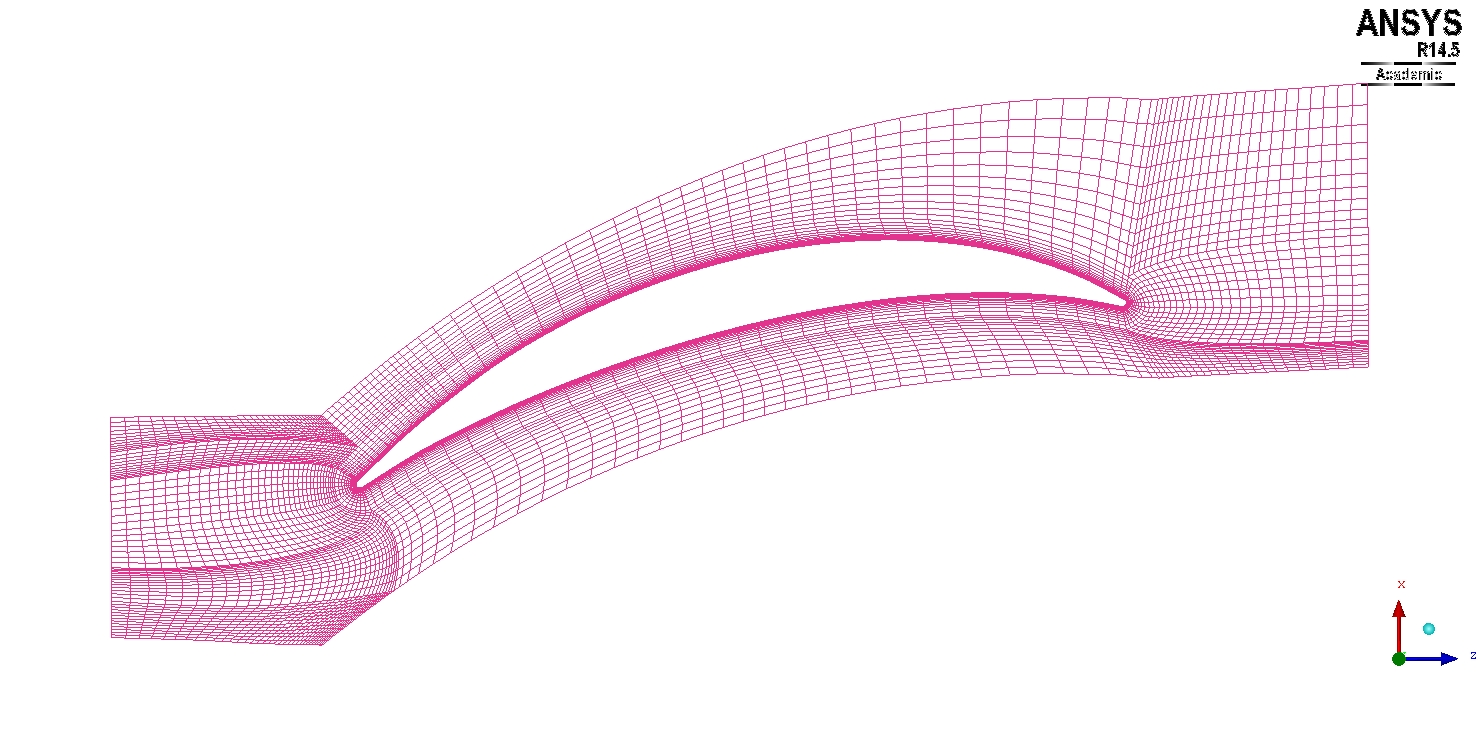
\includegraphics[width=0.85\textwidth]{Pictures/r67_cj.jpg}
\caption{Mesh topology with conforming periodic boundaries}
\label{cj_topo}
\end{figure}

Final topology was a standard h-grid topology for generic airfoils (fig. \ref{h_topo}). Although it is impossible to create a conforming periodic interface with such mesh topology, a fully structural tip gap was implemented. Omitting the blade-hub juncture fillet simplified the mesh.  Such topology eradicates the necessity of placing 5-way topology points.

\begin{figure}[h!]
\centering % bo \centering nie wstawia dodatkowego odstępu
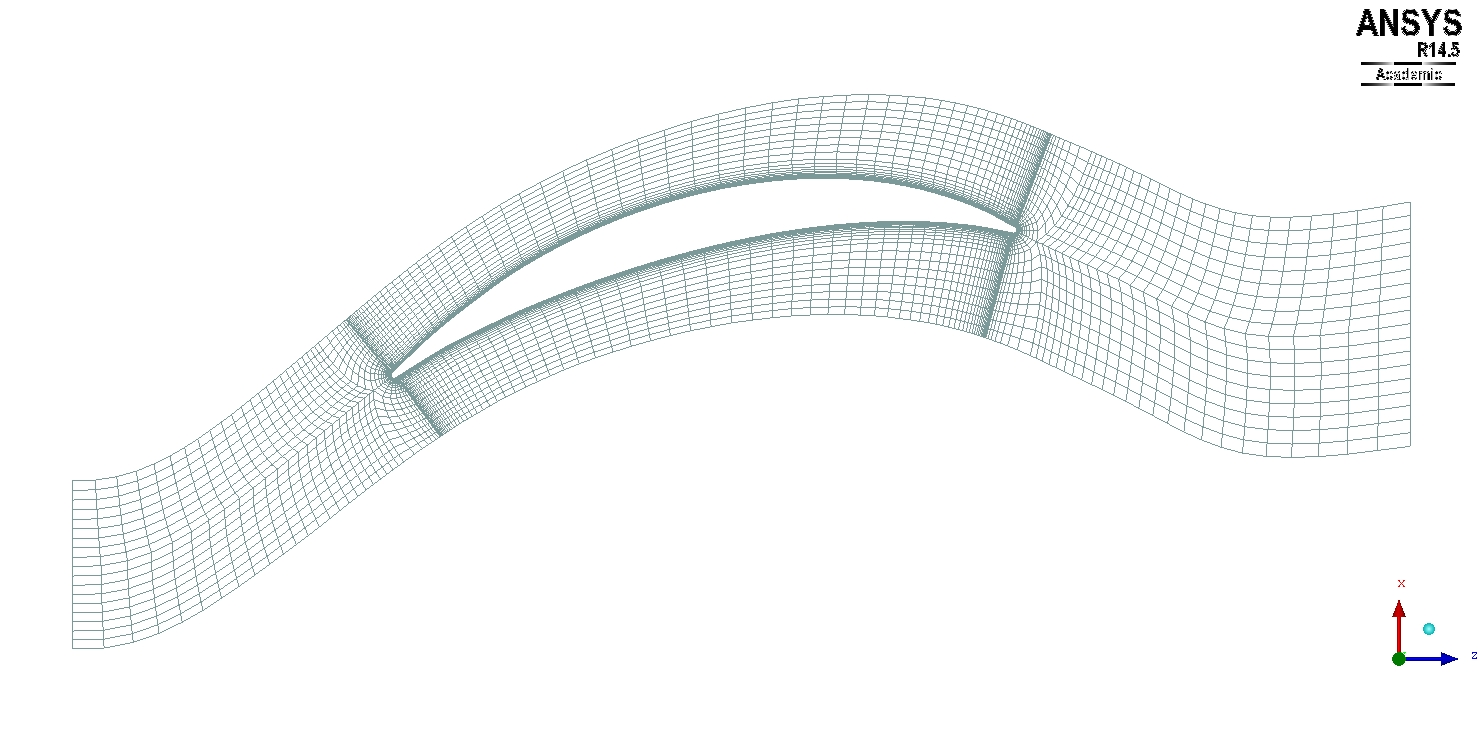
\includegraphics[width=0.85\textwidth]{Pictures/r67_htopo.jpg}
\caption{Mesh h-topology}
\label{h_topo}
\end{figure}

%Mesh was created in Ansys ICEM software using structural blocking method. The topology was sliced and associated to internal surfaces mentioned in the above section. This enforces mesh layering along design streamlines and provides high quality mesh on internal surfaces for flow field data acquisition further in the process. Blade wall boundary condition is distributed among five separate parts: blade pressure side, blade suction side, leading and trailing edges and tip surface. 

As there were no information about the frequency of the pressure fluctuations at time of creating the mesh, the analysis will focus on the audible range of sound frequencies from 20Hz to 20 000Hz. The wavelengths for given frequencies are calculated by formula \ref{eq:wl} and divided by four to obtain the required cell sizing. The velocity of sound obtained by equation \ref{eq:sos} with reference temperature $T = 300K$. The results are presented in table \ref{tab:meshsize}.

\begin{table}[htb!]
\centering
\caption{Test case boundary conditions} \label{tab:meshsize}
\begin{tabular}{@{}rll@{}}
\toprule
Frequency [Hz] & Wave length [m] & Cell size [m] \\ \midrule
20 & 17.390 & 4.347  \\
20 000 & 0.01739 & 0.004347 \\
\bottomrule
\end{tabular}
\end{table}

Maximum element edge length is limited to 3 mm, with 5 mm at inlet and outlet boundary conditions. The mesh cell sizing requirements are described in chapter \ref{approach}.  Blade boundary layer is produced by creating an o-grid around blade surface mesh. Hub and casing boundary layers are created by changing the sizing on the blocks adjacent to respective surface mesh. Sizing of the first element is estimated with y+ parameter as described in equation: \ref{eq:yplus}. First element thickness in on the blade surfaces ranges from is $2 \mu m$ on tip airfoil and $10 \mu m$ on hub airfoil. This corresponds to $y^{+} \approx 2$ calculated by streamline velocity values given in experimental study \citep{r67laser}.

\begin{equation} \label{eq:yplus}
\Delta s = \frac{y^{+} \mu}{U_{fric} \rho}
\end{equation}

\noindent where:
\begin{equation}
U_{fric} = \sqrt{\frac{\tau_{wall}}{\rho}}
\end{equation}

\noindent where:
\begin{equation}
\tau_{wall} = \frac{C_f \rho U_{\infty}^{2}}{2}
\end{equation}

\noindent where:
\begin{equation}
C_f = \frac{0.026}{Re_{x}^{1/7}}
\end{equation}

Internal volume of the mesh was stabilized by attaching the mesh blocks to the internal design surfaces, which represent the design streamline surfaces of the experimental rotor. This ensures that mesh layers are mostly coincident with the primary flow streamlines. The internal surface mesh is also used for data acquisition purposes. The markers are named \texttt{hub}, \texttt{int-01} thru \texttt{int-12} and \texttt{int-tip} corresponding to following locations of the design surfaces. The span percentage is calculated from the hub.

\begin{table}[htb!]
\centering
\caption{Location of compressor desing surfaces} \label{tab:surfs}
\ttfamily
\begin{tabular}{@{}rl@{}}
\toprule
Boundary marker & Location \\ \midrule
hub & 0\% span  \\
int-01 -- int-12 & 7.7\% -- 92.3\% every 7.7\% span \\
int-tip & 100\% span \\
\bottomrule
\end{tabular}
\end{table}

Figure \ref{mesh-ortho} provides overview of mesh quality defined above. The quality of created mesh is sufficient for both RANS and DDES analyses (chapter \ref{cfd}). Final mesh reached c.a. 11.5 million cell count. Final mesh is presented in figure \ref{meshfinal} 

\begin{figure}[h!]
\centering % bo \centering nie wstawia dodatkowego odstępu
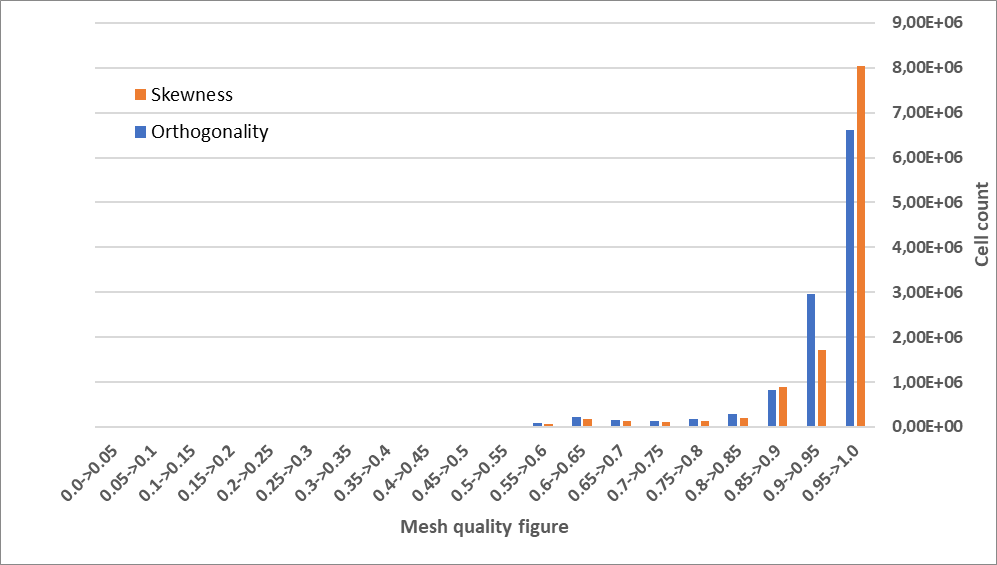
\includegraphics[width=0.85\textwidth]{Pictures/mesh_ortho.png}
\caption{Mesh quality histogram}
\label{mesh-ortho}
\end{figure}

\begin{figure}[t!]
\centering % bo \centering nie wstawia dodatkowego odstępu
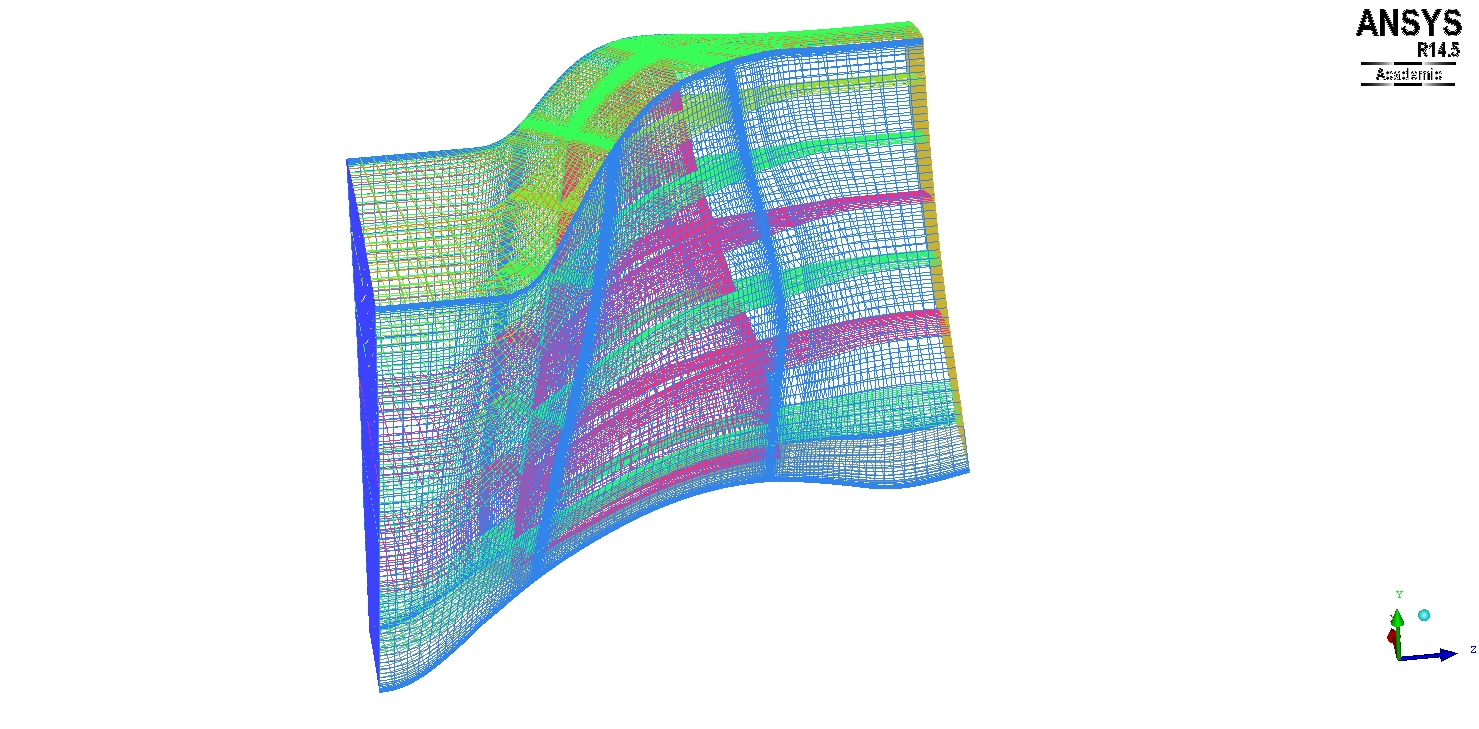
\includegraphics[width=0.85\textwidth]{Pictures/r67_ransmesh.jpg}
\caption{Completed Mesh}
\label{meshfinal}
\end{figure}

%----------------------------------------------------------------------------------------
%	SECTION
%----------------------------------------------------------------------------------------
%\section{Data acquisition} \label{casedata}
%Mesh and case is set up for possibly efficient data acquisition of flow field pressure and velocity data. FLUENT data file from a single timestep takes around 2GB of disk space. Saving such dataset from every of 50150 timesteps requires about 97TB of storage, which was unavailable at the time. 
%
%Data was gathered from blade surface (5 boundary markers) and 13 internal markers. Following node data values were saved:
%
%\begin{itemize}
%\item Static pressure
%\item Velocity magnitude (only internal markers)
%\item Vorticity magnitude (only internal markers)
%\item Static density
%\item Static temperature
%\item Node coordinates
%\end{itemize}
%
%This approach generated 18 datasets of 50510 files each, resulting in taking up 5.5TB of HPC cluster storage. The number of data is still large but manageable with current software engineering tools. Data was saved to ASCII text files.
% Chapter Template

\chapter{CFD Analysis} % Main chapter title

\label{cfd} % Change X to a consecutive number; for referencing this chapter elsewhere, use \ref{ChapterX}

\lhead{\emph{CFD analysis}} % Change X to a consecutive number; this is for the header on each page - perhaps a shortened title

%----------------------------------------------------------------------------------------
%	SECTION
%----------------------------------------------------------------------------------------
\section{Case preprocessing} \label{casepre}

CFD analyses for generating raw pressure field data are performed in ANSYS Fluent 17.2 software on Prometheus HPC cluster located in Kraków. Access for this infrastructure was granted by PLGrid infrastructure. Calculations were run on 5 nodes of 24CPU cores and 128GB RAM each \citep{prometheus}, which resulted in decomposition to 120 cores, resulting in allocating around 110 thousand cells to a single CPU core.

The analysis is set to "peak efficiency" conditions of the experimental test case. Apart from the turbulence modeling approach, the set up is consistent throughout the CFD cases.

Material used in the analysis resembles standard air modeled as ideal gas as in equation with following properties described in table \ref{tab:stdair} 

\begin{table}[ht!]
\centering
\caption{Standard air properties} \label{tab:stdair}
%\ttfamily
\begin{tabular}{@{}lrl@{}}
\toprule
$C_p$ & 1006.43 & J/(kg $\cdot$ K) \\
$\lambda$ & 0.0242 & W/(m $\cdot$ K \\
$\mu$ & $1.7894 \cdot 10^{-5}$ & kg/(m $\cdot$ s) \\
$M$ & 28.966 & kg/kmol \\
\bottomrule
\end{tabular}
\end{table}

\begin{equation} \label{eq:stadair}
p V = n R T
\end{equation}

Analysis operating pressure is set to 0 Pascal, which is a standard practice in compressible flow CFD. Internal mesh zone is set as "frozen rotor" reference frame. Although no mesh motion is implied, the effect of Coriolis accelerations and centrifugal acceleration will be taken into account by adding respective acceleration components to momentum equations as described in chapter \ref{approach}. The rotational velocity is set to 1680 rad/s.

Following boundary conditions were applied. The setup is typical for compressible flow CFD cases performed in the authors institute.

\begin{table}[htb!]
\centering
\caption{Test case boundary conditions} \label{tab:testbcs}
\ttfamily
\begin{tabular}{@{}llrl@{}}
\toprule
Boundary marker & Boundary type & & \\ \midrule
Inlet & Pressure Inlet & 101350  & Pa\\
Outlet & Pressure Outlet & 102000 & Pa \\
Hub & Movig wall & 1680 & rad/s \\
Blade & Moving wall & 1680 & rad/s \\
Casing & Stationary wall & &  \\
Internal profiles & Internal & & \\
Periodic boundaries & Interface & & \\ \bottomrule
\end{tabular}
\end{table}

%Moving wall boundaries represent the rotational velocity of the compressor blade and are necessary for stationary reference frame formulation. Boundary condition setup is no different to usual setups of analyses of such kind.

\section{Flowfield initialization \& RANS}
RANS analysis is not suitable for generating acoustic nearfield data as the method averages the fluctuations over time (chapter \ref{approach}). Yet, this approach is used to solve the initial flowfield at a relatively low computational effort. Furthermore the RANS analysis provides initial validation results of the model setup and solver settings.

The solver is set up to steady-state, density based, coupled-implicit solver with $k-\omega \, SST$ turbulence model. Such setup is a go-to setup for nearly all compressible aerodynamics CFD done in the author's institute.

The density-based solver in ANSYS Fluent solves the governing equations of continuity, momentum, and (where appropriate) energy and species transport simultaneously as a set, or vector, of equations. Governing equations for additional scalars will be solved sequentially (that is, segregated from one another and from the coupled set). Two algorithms are available for solving the coupled set of equations, the coupled-explicit formulation and the coupled-implicit formulation \citep{fluenttheory}.

The system of governing equations for a single-component fluid, written to describe the mean flow properties, is cast in integral Cartesian form for an arbitrary control volume $V$ with differential surface area $dA$ as follows:

\begin{equation} \label{eq:densitybased}
\frac{\partial}{\partial t} \int_V WdV + \oint_V \left[ F-G \right] \cdot dA = \int_V HdV
\end{equation}

\noindent where:

\begin{equation} \label{eq:desityvectors}
\begin{aligned}
	W &= \begin{bmatrix}
		\rho \\
		\rho u \\
		\rho v \\
		\rho w \\
		\rho E
	\end{bmatrix}
\end{aligned} \quad
\begin{aligned}
	F &= \begin{bmatrix}
		\rho v\\
		\rho uv + pi\\
		\rho vv + pj\\
		\rho wv + pk\\
		\rho vE + pv
	\end{bmatrix}
\end{aligned} \quad
\begin{aligned}
	G &= \begin{bmatrix}
		0 \\
		\tau_{xi} \\
		\tau_{yi} \\
		\tau_{zi} \\
		\tau_{ij} v_j + q
	\end{bmatrix}
\end{aligned}
\end{equation}

\noindent and where the vector $H$ is the body forces and energy source vector.

The $\rho, v, E, p$ are respectively the density, velocity, total energy per unit mass and pressure of the fluid. $\tau$ is the viscous stress tensor and $q$ is the heat flux.

Total energy $E$ and total enthalpy $H$ are related by the formulas:

\begin{equation} \label{eq:totalenergy}
E = H - \frac{p}{\rho}
\end{equation}

\begin{equation} \label{eq:totalenthalpy}
H = h + \frac{\lvert v \rvert^2}{2} 
\end{equation}

Equation \ref{eq:densitybased} is preconditioned, convective fluxes are splitted with Roe Flux-Difference Scheme and the preconditioned equation is discreticized with Euler Implicit discretization and combined with Newton type linearization of fluxes. Obtained equation system is solved by the Incomplete Lower Upper (ILU) factorization in conjunction with the Algebraic-Multi-Grid. Details on the solver theory used in this study are available in source \citep{fluenttheory}

Flowfield is initialized at first with constant values populated from the "inlet" boundary condition patch. Next a Full-Multi-Grid initialization is performed to generate coarsened flowield. The analysis is then processed by first, second and third order discretization schemes for all of the conservation values, up to a given residual value. It must be noted, that for second and third order scheme analyses, convergence criteria may not be reached. Should this case occur, the analysis is stopped once the residual plots reach a plateau and the resulting flowfield is considered acceptable. Once the third order scheme analysis is completed, data is acquired from inlet and outlet boundary conditions, and the constant pitch vs. span streamlines.

The analysis is set to a moderately strict residual convergence criteria of $10^{-6}$, however is monitored during runtime. Once the convergence plot reaches plateau and the internal surfaces flow field is not changing throughout iterations the analysis is stopped and switched to a higher discretization scheme or finalized and saved.

%----------------------------------------------------------------------------------------
%	SECTION
%----------------------------------------------------------------------------------------
\section{DDES analysis}
Once the RANS analysis is converged to a satisfactory level the setup is changed to a transient, pressure-based, PISO scheme solver with DDES turbulence model and $k-\omega \, SST$ RANS formulation for shielded regions and subgrid scale. Rationale for the DDES analysis is provided in chapter \ref{approach}. Pressure based solver is required by the DDES implementation in the used software. Utilization of the pressure based solvers for compressible flows is known to be unstable during the calculations, especially for the adverse pressure gradient cases. However, once the initial flow field resembles the final flowfield, the pressure based calculations are rather stable even at high velocity adverse pressure gradients.

Pressure based solver solves the discretized continuity equation with obtaining the velocity field from the momentum equations. The pressure field is obtained by solving and manipulating the continuity and momentum equations within a pressure velocity coupling scheme.

%Special practices for treatment of the continuity (\ref{eq:cont}) and momentum (\ref{eq:momentum}) equations are described for mentioned equations is integral form (equations \ref{eq:cont_int} and \ref{eq:momentum_int} respectively).
%
%\begin{equation} \label{eq:cont_int}
%\oint \rho \vec{v} \cdot d \vec{A} = 0
%\end{equation}
%
%\begin{equation} \label{eq:momentum_int}
%\oint \rho \vec{v} \vec{v} \cdot d \vec{A} = -\oint pI \cdot d \vec{A} + \oint \overline{\overline{\tau}} \cdot d \vec{A} + \int_V \vec{F}dV
%\end{equation}

Transformed and discretized equations are solved by a linear solver and the intermittent solutions are coupled using a pressure velocity coupling algorithm. For this specific case PISO scheme is chosen for the computation. The algorithm is suitable for calculating problems with larger (in comparison to density-based acoustical timescale) pseudo-timestep and with decreased computational expense. Figure \ref{piso} presents the flow of the PISO algorithm. 

%\begin{figure}[h!]
%\centering % bo \centering nie wstawia dodatkowego odstępu
%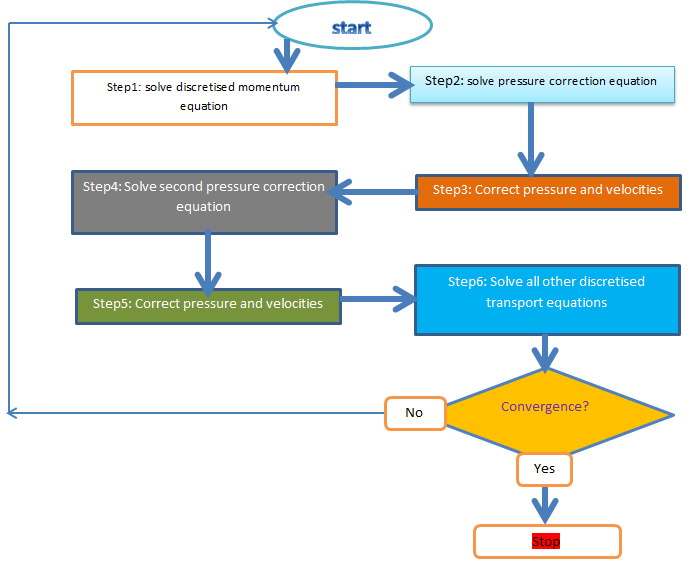
\includegraphics[width=0.85\textwidth]{Pictures/PISO.png}
%\caption{Flowchart of the PISO algorithm}
%\label{piso}
%\end{figure}

\begin{figure}[h!]
\centering % bo \centering nie wstawia dodatkowego odstępu
\usetikzlibrary{positioning}
\tikzstyle{decision} = [diamond, draw, aspect=2, text width=7em, text centered, node distance=1cm, inner sep=0pt]
\tikzstyle{block} = [rectangle, draw, text width=8em, text centered, node distance=1cm, rounded corners, minimum height=3em]
\tikzstyle{line} = [draw, -latex]
\tikzstyle{cloud} = [draw, ellipse, node distance=1cm, minimum height=3em]

\begin{tikzpicture}[node distance = 2cm, auto]
    % Place nodes
    \node [cloud] (start) {Start};
    \node [block, right=0.85cm of start] (step_one) {1: Solve the discretized momentum equation};
    \node [block, right=0.85cm of step_one] (step_two) {2: Solve the pressure correction equation};
    \node [block, right=0.85cm of step_two] (step_three) {3: Correct pressure and velocities};
    \node [block, below=1cm of step_three] (step_four) {4: Solve second pressure correction equation};
    \node [block, left=0.85cm of step_four] (step_five) {5: Correct pressure and velocities};
    \node [block, below=0.85cm of step_five] (step_six) {6: Solve all other transport equations};
    \node [decision, left=0.85cm of step_six] (convergence) {Converged?};
    \node [cloud, left=0.85cm of convergence] (stop) {Stop};
    % Draw edges
    \path [line] (start) -- (step_one);
    \path [line] (step_one) -- (step_two);
    \path [line] (step_two) -- (step_three);
    \path [line] (step_three) -- (step_four);
    \path [line] (step_four) -- (step_five);
    \path [line] (step_five) -- (step_six);
    \path [line] (step_six) -- (convergence);
    \path [line] (convergence.north) -- node {no} (step_one);
    \path [line] (convergence.west) -- node {yes} (stop);   
\end{tikzpicture}
\caption{Flowchart of the PISO algorithm}
\label{piso}
\end{figure}

%\tikzstyle{decision} = [diamond, draw, text width=10em, text centered, node distance=4cm, inner sep=0pt]
%\tikzstyle{block} = [rectangle, draw, text width=10em, text centered, node distance=4cm, rounded corners, minimum height=3em]
%\tikzstyle{line} = [draw, -latex]
%\tikzstyle{cloud} = [draw, ellipse, node distance=3cm, minimum height=3em]
%
%\begin{tikzpicture}[node distance = 2cm, auto]
%    % Place nodes
%    \node [cloud] (start) {Start};
%    \node [block, below of=start] (step_one) {1: Solve the discretized momentum equation};
%    \node [block, right of=step_one] (step_two) {2: Solve the pressure correction equation};
%    \node [block, below of=step_two] (step_three) {3: Correct pressure and velocities};
%    \node [block, left of=step_three] (step_four) {4: Solve second pressure correction equation};
%    \node [block, below of=step_four] (step_five) {5: Correct pressure and velocities};
%    \node [block, right of=step_five] (step_six) {6: Solve all other transport equations};
%    \node [decision, below of=step_five] (convergence) {Convergence?};
%    \node [cloud, below of=convergence] (stop) {Stop};
%    % Draw edges
%    \path [line] (start) -- (step_one);
%    \path [line] (step_one) -- (step_two);
%    \path [line] (step_two) -- (step_three);
%    \path [line] (step_three) -- (step_four);
%    \path [line] (step_four) -- (step_five);
%    \path [line] (step_five) -- (step_six);
%    \path [line] (step_six) |- (convergence);
%    %\path [line] (convergence) -- [near start] node {no} (step_one);
%    \path [line] (convergence) -- node {yes} (stop);   
%\end{tikzpicture}

As the flowfield resulting from the RANS analysis is averaged over time and has no distinguishable features of a turbulent flow, the DDES analysis is divided into two runs. The first run is set to create a flowfield with random flow features. This is also used for testing the convergence and data acquisition process.

Although not required by the "frozen-rotor" configuration, the timestepping is based on the rotor Blade-Pass-Frequency number. The BPF parameter is obtained by formula \ref{eq:bpf}

\begin{equation} \label{eq:bpf}
BPF = \frac{n \cdot t}{60}
\end{equation}

\noindent where $t$ is the number of blades and $n$ is the rotational speed in rpm.

For NASA R67 the base Blade Passing Frequency is equal to $5882.36 Hz$. By multiplying the BPF by four a frequency of $23529.44 Hz$ is obtained. The frequency is above the human audible range and will be used to compute the timestep. As stated in chapter \ref{approach}, in order to capture a given frequency, the timestep must be at least 4 times smaller than the period of the oscillations (equation \ref{eq:mintime}). By this approach the maximum timestep of the DDES calculation is $1.06 \cdot 10^{-5}s$. The timestep is compared with the requirements of the Courant-Friedrichs-Levy condition defined by equation \ref{eq:CFL}

\begin{equation} \label{eq:CFL}
Co = \frac{u \cdot \Delta t}{\Delta x}
\end{equation}

Considering that $u_{max} = 426.72 m/s$ and $\Delta x = 0.25 \cdot \lambda = 0.003695 m$ for desired frequency of $23529.44 Hz$ and timestep of  $1.06 \cdot 10^{-5}s$ the Courant number obtained is equal to 1.22. By rearranging the equation to solve for $\Delta t$ an equation \ref{eq:CFL2} is obtained and a calculation timestep fulfilling requirements of the CFD analysis and the direct noise formulation is computed and is equal to $8.659 \cdot 10^{-6}$.

\begin{equation} \label{eq:CFL2}
\Delta t = \frac{Co \cdot \frac{\lambda}{4}}{u_{max}}
\end{equation}

Initial timestep for the DDES analysis is set up to $5.0 \cdot 10^{-6}s$. Presented time stepping approach fulfills the Shannon-Nyquist-Whitaker theorem presented in section \ref{timestepsize}. First run was conducted for c.a. 30 thousand timesteps, during which following factors were tested: calculation efficiency dependent on the CPU core count used, data output and data format, estimated storage requirements and the output from the embedded FW-H aeroacoustical models. First run concluded, that the assumed timestep does not meet the required convergence criteria and delivered inaccurate results or flowfield with features not resembling the features characteristic for compressor flow.

The timestep was gradually decreased to a value of $1.0 \cdot 10^{-6}s$, the CPU core count was set to 120 CPU cores distributed over 5 HPC nodes. Once the first run produced a fully developed flowfield with turbulent features characteristic to the LES analysis, the case was saved and set up for a final run with full data acquisition. 

It was desired to capture at least 0.05 seconds of the flow but with some relation to geometric and operational features of the rotor. Based on the blade count and rotational speed of the rotor a time of a single periodic passage is calculated to $1.70 \cdot 10^{-4}s$. Next the required computational time is divided by the passage time to obtain the number of blade passages. 294.118 passages will occur during the 0.05s, so the number is rounded up to 295 passages and multiplied again by the passage time. Total calculation time of 0.05015 seconds is obtained. Therefore 50150 timesteps is required for full calculation runtime, with one passage being calculated in 170 timesteps.

%-----------------------------------
%	SECTION
%-----------------------------------
\section{Validation of the results}
The experimental study \citep{r67laser} provides a very extensive set of validation data for the passage flowfield. The quoted study presents results of LDA measurements of the NASA R67 compressor for relative mach number and relative flow angle at constant pitch and constant chord lines intersecting with blade span lines at 10\% intervals. Constant pitch line is derived from the blade's suction surface: 0\% percent pitch is the suction surface of one blade, 100\% pitch is the suction surface of the adjacent blade. Constant chord lines are used to plot blade-to-blade distributions of given parameters at intersection of span and constant z-coordinate surface (fig. \ref{fig_LA}).

\begin{figure}[h!]
\centering % bo \centering nie wstawia dodatkowego odstępu
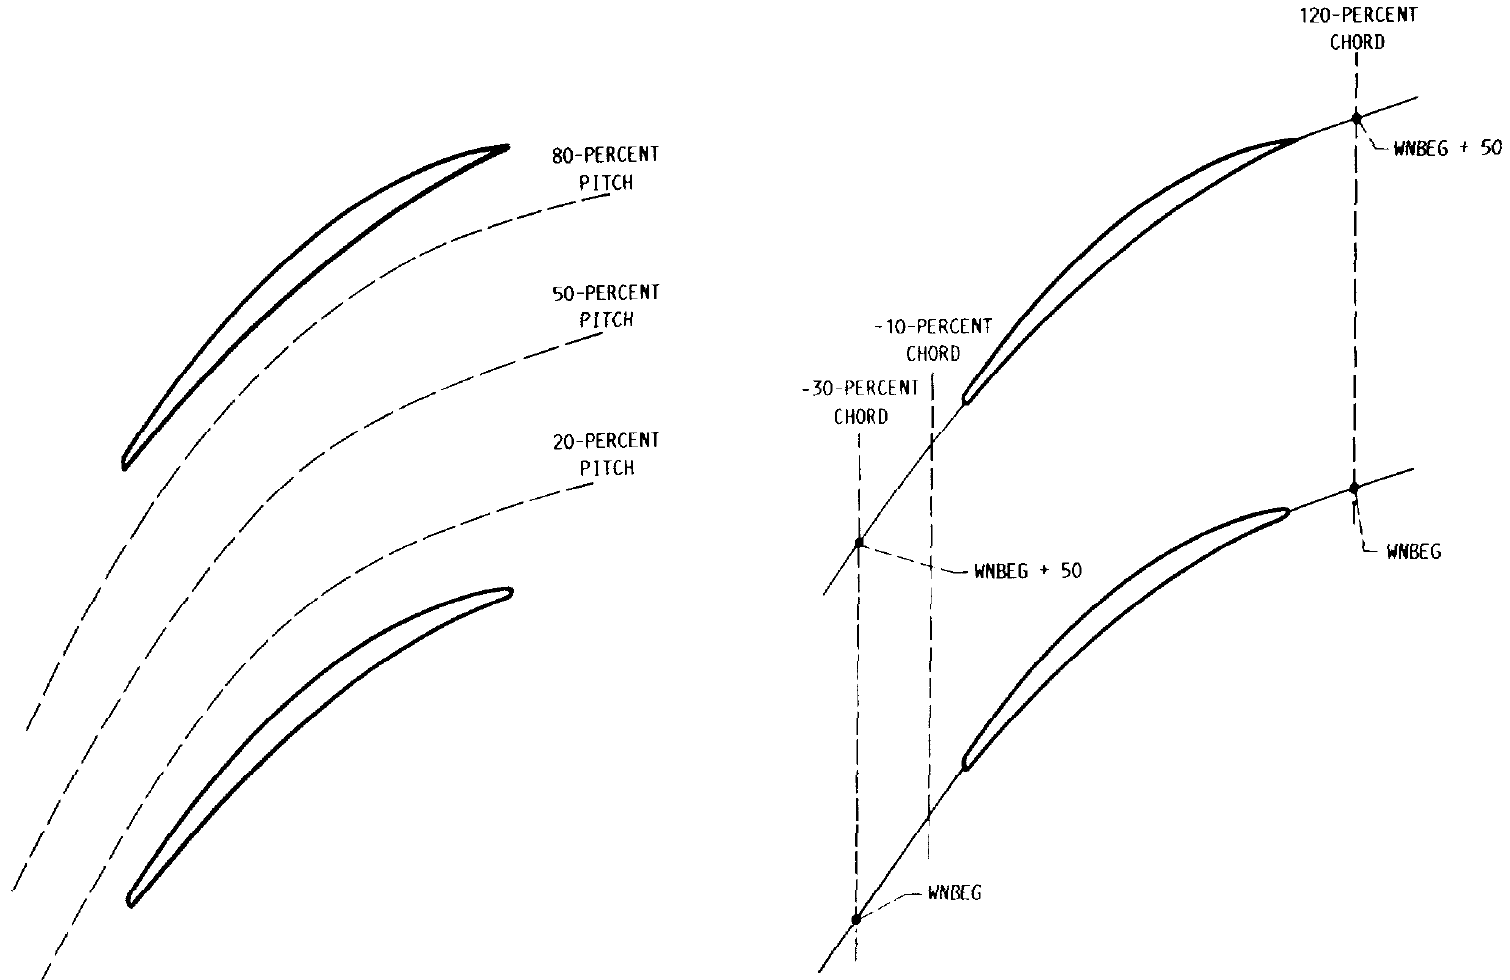
\includegraphics[width=0.85\textwidth]{Pictures/LA.png}
\caption{Schematic representation of constant pitch (left) and constant chord (right) to plot data \citep{r67laser}}
\label{fig_LA}
\end{figure}

In order to validate the CFD analysis, the constant pitch surfaces for 20\%, 50\% and 80\% constant pitch are combined with 10\%, 50\% and 90\% constant span locations, as measured from the blade tip, thus producing 9 lines to for relative Mach number and relative flow angle data. Furthermore, Mach contour plots for 10\%, 30\% and 70\% constant span surfaces (measuring from the blade tip) are compared with the experimental study.

For clarity, relative mach number plots and constant pitch plots are presented in appendix \ref{cfd_results}. 

The most simple method for validating the results is comparing the total and static pressure values on inlet and outlet boundary conditions of the domain with experimental data. Plots for static and total pressure at inlets and outlets of the domain are presented in figures \ref{pvalid_in} and \ref{pvalid_out}. 

\begin{figure}[h!]
\centering % bo \centering nie wstawia dodatkowego odstępu
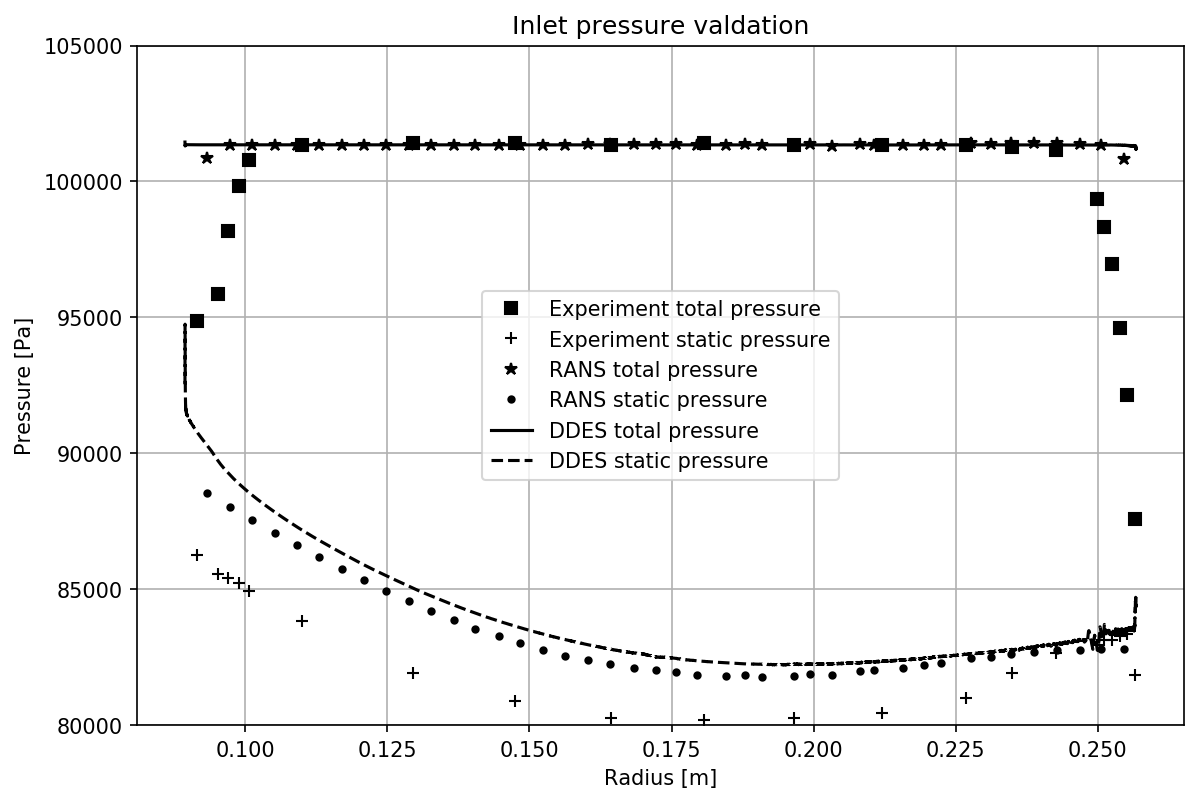
\includegraphics[width=0.8\textwidth]{Pictures/pvalid_in.png}
\caption{Inlet pressure validation}
\label{pvalid_in}
\end{figure}

\begin{figure}[h!]
\centering % bo \centering nie wstawia dodatkowego odstępu
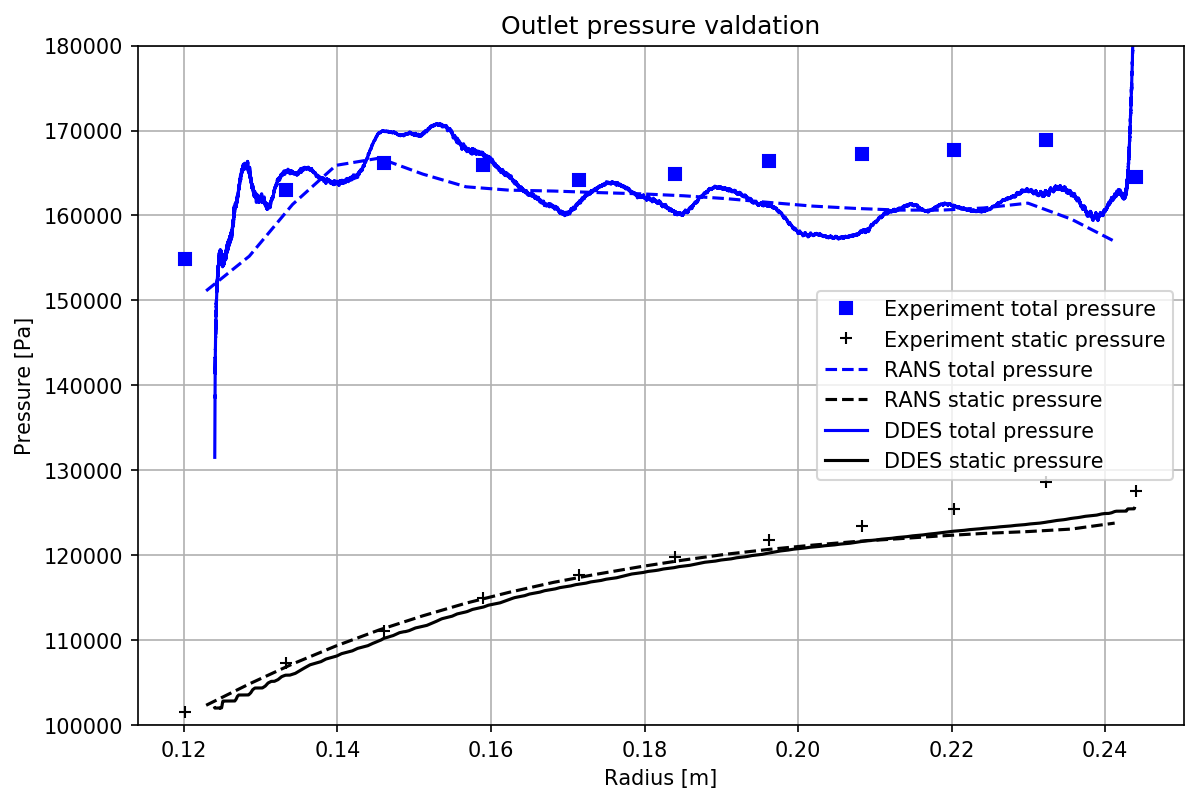
\includegraphics[width=0.8\textwidth]{Pictures/pvalid_out.png}
\caption{Outlet pressure validation}
\label{pvalid_out}
\end{figure}

%\begin{figure}[h!]
%\centering % bo \centering nie wstawia dodatkowego odstępu
%
\includegraphics[width=0.85\textwidth]{Pictures/placeholder.jpg}
%\caption{DDES analysis inlet pressure validation}
%\label{pvalid_ddes_in}
%\end{figure}
%
%\begin{figure}[h!]
%\centering % bo \centering nie wstawia dodatkowego odstępu
%
\includegraphics[width=0.85\textwidth]{Pictures/placeholder.jpg}
%\caption{DDES analysis outlet pressure validation}
%\label{pvalid_ddes_out}
%\end{figure}

Both RANS and DDES analyses produce results that are confirmed by the experimental data. Static inlet pressure plot show the discrepancy between experimental and CFD data resulting from a minor shift between the inlet and outlet CFD boundaries and the location of the pressure rake. The inlet boundary condition is moved closer towards the leading edge of the rotor, than the experimental pressure measurements array, therefore the static pressure is increased. The Mach number contour plots on the corresponding internal surfaces show the same character of the flow. Discrepancies between the experimental study and the obtained CFD results arise from a slight offset between the experimental surfaces as the mesh internal surfaces.  
% Chapter Template

\chapter{Results of flow field noise analysis} % Main chapter title

\label{results} % Change X to a consecutive number; for referencing this chapter elsewhere, use \ref{ChapterX}

\lhead{\emph{Results of flow field noise analysis}} % Change X to a consecutive number; this is for the header on each page - perhaps a shortened title

%----------------------------------------------------------------------------------------
%	SECTION 1
%----------------------------------------------------------------------------------------

\section{Main Section 1}

Lorem ipsum dolor sit amet, consectetur adipiscing elit. Aliquam ultricies lacinia euismod. Nam tempus risus in dolor rhoncus in interdum enim tincidunt. Donec vel nunc neque. In condimentum ullamcorper quam non consequat. Fusce sagittis tempor feugiat. Fusce magna erat, molestie eu convallis ut, tempus sed arcu. Quisque molestie, ante a tincidunt ullamcorper, sapien enim dignissim lacus, in semper nibh erat lobortis purus. Integer dapibus ligula ac risus convallis pellentesque.

%-----------------------------------
%	SUBSECTION 1
%-----------------------------------
\subsection{Subsection 1}

Nunc posuere quam at lectus tristique eu ultrices augue venenatis. Vestibulum ante ipsum primis in faucibus orci luctus et ultrices posuere cubilia Curae; Aliquam erat volutpat. Vivamus sodales tortor eget quam adipiscing in vulputate ante ullamcorper. Sed eros ante, lacinia et sollicitudin et, aliquam sit amet augue. In hac habitasse platea dictumst.

%-----------------------------------
%	SUBSECTION 2
%-----------------------------------

\subsection{Subsection 2}
Morbi rutrum odio eget arcu adipiscing sodales. Aenean et purus a est pulvinar pellentesque. Cras in elit neque, quis varius elit. Phasellus fringilla, nibh eu tempus venenatis, dolor elit posuere quam, quis adipiscing urna leo nec orci. Sed nec nulla auctor odio aliquet consequat. Ut nec nulla in ante ullamcorper aliquam at sed dolor. Phasellus fermentum magna in augue gravida cursus. Cras sed pretium lorem. Pellentesque eget ornare odio. Proin accumsan, massa viverra cursus pharetra, ipsum nisi lobortis velit, a malesuada dolor lorem eu neque.

%----------------------------------------------------------------------------------------
%	SECTION 2
%----------------------------------------------------------------------------------------

\section{Main Section 2}

Sed ullamcorper quam eu nisl interdum at interdum enim egestas. Aliquam placerat justo sed lectus lobortis ut porta nisl porttitor. Vestibulum mi dolor, lacinia molestie gravida at, tempus vitae ligula. Donec eget quam sapien, in viverra eros. Donec pellentesque justo a massa fringilla non vestibulum metus vestibulum. Vestibulum in orci quis felis tempor lacinia. Vivamus ornare ultrices facilisis. Ut hendrerit volutpat vulputate. Morbi condimentum venenatis augue, id porta ipsum vulputate in. Curabitur luctus tempus justo. Vestibulum risus lectus, adipiscing nec condimentum quis, condimentum nec nisl. Aliquam dictum sagittis velit sed iaculis. Morbi tristique augue sit amet nulla pulvinar id facilisis ligula mollis. Nam elit libero, tincidunt ut aliquam at, molestie in quam. Aenean rhoncus vehicula hendrerit.
% Chapter Template

\chapter{Conclusions \& Further work} % Main chapter title

\label{conclusions} % Change X to a consecutive number; for referencing this chapter elsewhere, use \ref{ChapterX}

\lhead{\emph{Conclusions \& Further work}} % Change X to a consecutive number; this is for the header on each page - perhaps a shortened title

%----------------------------------------------------------------------------------------
%	SECTION
%----------------------------------------------------------------------------------------
\section{Results discussion}
Initially, this thesis intended to investigate the following phenomena on a fan blade of a commercial large by-pass-ratio turbofan engine blade, yet no information on airfoil coordinates and efficiency figures of such devices are available for research purposes. It is assumed, that the phenomena that occur on such blade are similar in character to the ones obtained on the provided test case. Although the practical utilization of presented results is limited at this stage, some conclusion can be drawn out. The approach used on a NASA R67 transonic axial compressor provide some insight to noise generation phenomena in a "frozen-rotor" reference frame. It must be noted, that noise perceived by human or received by a microphone will be different from the ones presented. However, the noise perceived has it's source in the phenomena discussed in this thesis.

The main contributors to the blade's noise generation are the boundary layer separations induced by backflow in the boundary layer or by the shockwave boundary layer interaction. The existence of a shockwave in a device of that kind is also the main contributor of the so-called "buzzsaw noise", which may be recognized by simulating a rotor with a moving mesh and with a stationary receiver or data probe. Largest, in terms of amplitude and frequency, sound pressure fluctuations are found at the trailing edge of the blade and at trailing edge-tip junction. Sound pressure in decibel scale as well as average frequency per node of control surface are in expected range for this kind of device.

Following assumptions can be made. In order to reduce the noise generated by the transonic axial compressor blade one must eradicate the sources of separated flow and, if possible, provide a supersonic to subsonic transition of flow without inducing a shockwave. At time of preparation of this thesis, methods for inverse design of boundary shapes based on pressure and/or other design criteria exist in open source domain. Such software allows for generating airfoils for fixed wing aircraft and rotating machinery. Furthermore, modification of shape of the blade trailing edge by implementing a shape that reduces the vortex shedding or at least the turbulence intensity in wake. At this stage, there are no suggestions for manipulating the frequency of the fluctuations.

Results of direct noise analysis on hub and casing surfaces are not presented due to a simple mistake -- these surfaces were  accidentally removed from the CFD solution export of the DDES analysis. Only one low frequency cycle is captured due to another mistake. As described in chapter \ref{cfd}, the timestep of the analysis was decreased by the order of magnitude in order to improve the analysis convergence. However, the solution export was still set up to deliver a dataset per timestep which resulted in a dataset 10 times larger than necessary, with no available walltime to continue the calculation.

The main downside of the presented study is lack of validation data for acoustical nearfield of the given case. It is assumed, that the approach is valid when two following factors coincide: if the CFD analysis that generate flow-field data is validated by experimental data and if FFT and RMS scripts return the expected results while the input is a sum of sine waves of known frequency, amplitudes and phase shifts. The CFD analysis results were validated with the experimental data provided in reference \citep{r67laser} as described in chapter \ref{cfd}, therefore it is assumed that the DDES flowfield data is valid. The RMS script return the expected average amplitude value while processing a set of sine wave signals, whereas the FFT script returned proper frequency spectrum and phase shift of the given signal. By this indirect validation, it is assumed that presented results are valid.

%----------------------------------------------------------------------------------------
%	SECTION
%----------------------------------------------------------------------------------------
\section{Improvements to the method}
Current approach may be compared to attempts of resolving a turbulent boundary layer with one finite volume element at the boundary wall. Although mathematically possible (and used in wall modeled turbulence models) it is valid under fulfilling some assumptions. For presented direct approach, it is assumed that sinusoidal fluctuation of wavelength enclosed by four finite volumes and resolved by four timesteps.

Resolving a sinusoidal fluctuation with four finite volumes and four timesteps fulfills the continuity and momentum equations, any change in temperature, resulting in changing velocity of sound will disrupt the assumptions presented in chapter \ref{approach}. FFT amplitude plots for ordinary frequencies, analyzed at random mesh points show, that the amplitudes of frequencies above the assumed by mesh and timestep range are dropped nearly to zero. A solution for this is using a finer mesh, capable of resolving shorter wavelength fluctuations, along with smaller timestepping to compensate for transition of sound wave in the finer mesh, especially in the boundary layer region and in the wake.

Considering that the mesh resolution is increased, a proper method for resolving turbulence flow is required. Although justified from the computational expense standpoint, the hybrid methods with shielding functions may result in filtering the source fluctuations at the boundary due to switching to the RANS part of given model. Using LES methods for further work will be considered.

Another aspect to be considered for improvement is the walltime management and data management. Presented analyses was performed on a Prometheus HPC and was distributed to 120 nodes. Normalized walltime for the analysis was above 1M CPU hours for both transition DDES and final DDES analyses and around 11TB of data was generated during the process. Using LES methods requires meshes of much greater density and therefore meshes of at least order of magnitude larger than used in this case. Assuming that walltime requirement is scaled linearly with the mesh size, assumed LES analysis of the presented test case, would have had required more than 10M CPU hours and around 1000CPU nodes.

Realtime processing of data to obtain sound information in the flowfield is impractical if even possible for full meshes, due to the amount of data generated. An efficient and high capacity storage storage is therefore required for performing direct approach analyses of sound on full flowfield.

Post-processing of data obtained in this study was performed with use of Matplotlib Pyplot library available for Python scripting language and hence the information about mesh was dropped during the process. This is visible especially in the internal surface scatter plots where lack of interpolation between points is visible. Using a post-processing tool with custom filters such as Paraview, or implementing a mesh file reader into Python (or any other implementation) scripts will solve problem with interpolation of data and allow visualization of full flowfield datasets.

\section{Further work}
As stated above, lack of validation case that directly checks the acoustical nearfield results is somewhat of a challenge. Therefore developing an experimental and numerical case of known acoustic nearfield properties is required. 

The implementation of mesh reading or mapping to mesh functionality will be developed in further versions of the post-processing scripts. This will allow for more efficient qualitative an quantitative analysis of the obtained data.

Presented work describes a single passage of the compressor in stationary reference frame ("Frozen rotor") configuration and gives insight to basic aerodynamic phenomena contributing to noise. In order to asses the noise generation in compressor, or fan, flows the analysis ought to be performed with use of rotating mesh with sliding interfaces and include effects of rotor-to-stator interaction, as well as interaction with compressor hub and casing. Furthermore, performing data acquisition and processing on full flow-field of the given case will give a better opportunity to post-process the obtained data. By extending the analysis time to more than 1 cycle of low frequency sound (0.05s), and preferably to more than five of such cycles, it may be possible to obtain information on acoustical wave modes within the flowfield of the case subject to study.

Considering that the geometry of given case is periodic, assuming the periodicity of flow in the DDES and LES analysis is prone to over constraining the resulting flowfield. Hence the analyses should be conducted on full rotor-stator stage, or at least a large portion of a stage, to eradicate or minimize the effect of periodic boundary conditions. This, combined with proposed LES simulation, enforces using a mesh with cell count in $10^8$ order of magnitude, which leads to further challenges with data management and required computational resources.

\section{Closing remarks}
The study presented in this thesis can be interpreted two-wise. One as a case study on direct formulation of noise analysis and providing the minimum requirements towards the analysis. Second aspect is the study of generating sound by the transonic axial compressor rotor blade. Both aspects of the study are, at least partially, fulfilled.

The provided minimum requirements of the analysis proved to work at relatively high computational expense. Yet, using the acoustical analogies implemented into used CFD code with transonic flows with shockwaves is unjustified by the mathematical formulation of the FW-H analogy. The resolution of the obtained acoustical nearfield can be improved at a cost of higher computational power requirements.

The presented results of the compressors acoustical nearfield are rather expected and are relateable to relative mach number fields and time averaged static pressure fields. Results identify the sources of aerodynamic noise that are consistent with ones described in literature, turbulent regions of the flow are the source of pressure fluctuations of high amplitude and high frequency. Propagation of sound waves was captured for lower end of the frequency spectrum, while the effect of high pitch noise is captured as an increase in RMS sound pressure and decibel figures. These results can be used to design a compressor blade that generates lower aerodynamically induced noise.

The method will be improved in terms of efficiency and data storage and attempted to be used in other technical entities where noise generation and acoustical wave mode assessment is required.

%----------------------------------------------------------------------------------------
%	THESIS CONTENT - APPENDICES
%----------------------------------------------------------------------------------------

%\addtocontents{toc}{\vspace{2em}} % Add a gap in the Contents, for aesthetics

\appendix % Cue to tell LaTeX that the following 'chapters' are Appendices

% Include the appendices of the thesis as separate files from the Appendices folder
% Uncomment the lines as you write the Appendices

%% Appendix Template

\chapter{RMS values plots} % Main appendix title

\label{rms_results} % Change X to a consecutive letter; for referencing this appendix elsewhere, use \ref{AppendixX}

\lhead{\emph{RMS values plots}} % Change X to a consecutive letter; this is for the header on each page - perhaps a shortened title

\begin{figure}[ht]
	\centering
	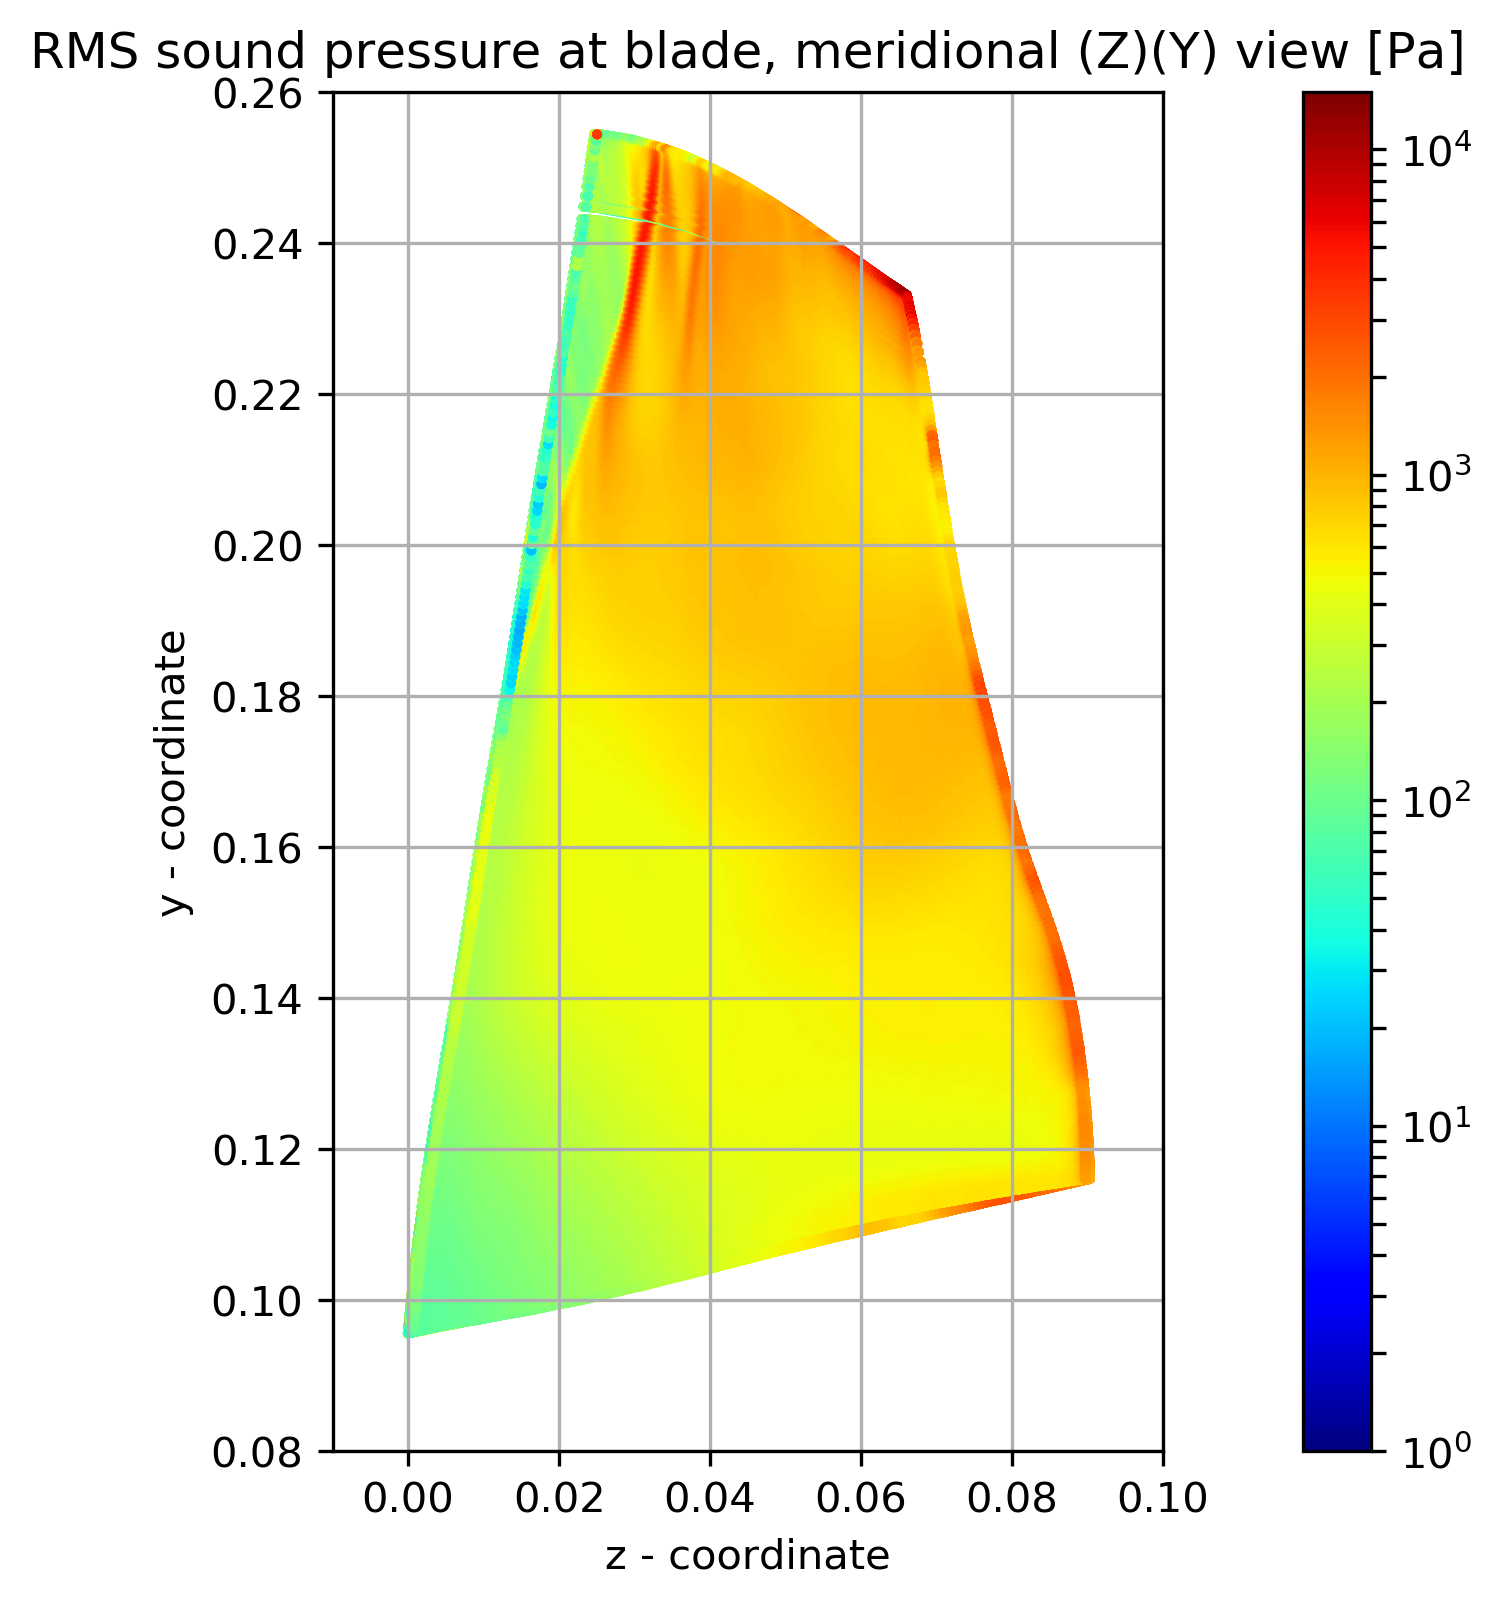
\includegraphics[width=0.85\textwidth]{Figures/blade-zy-rms-spl.png}
    \caption{RMS Sound pressure at blade (zy plane)} \label{blade-zy-rms-spl}
\end{figure}	

\begin{figure}[ht]
	\centering
	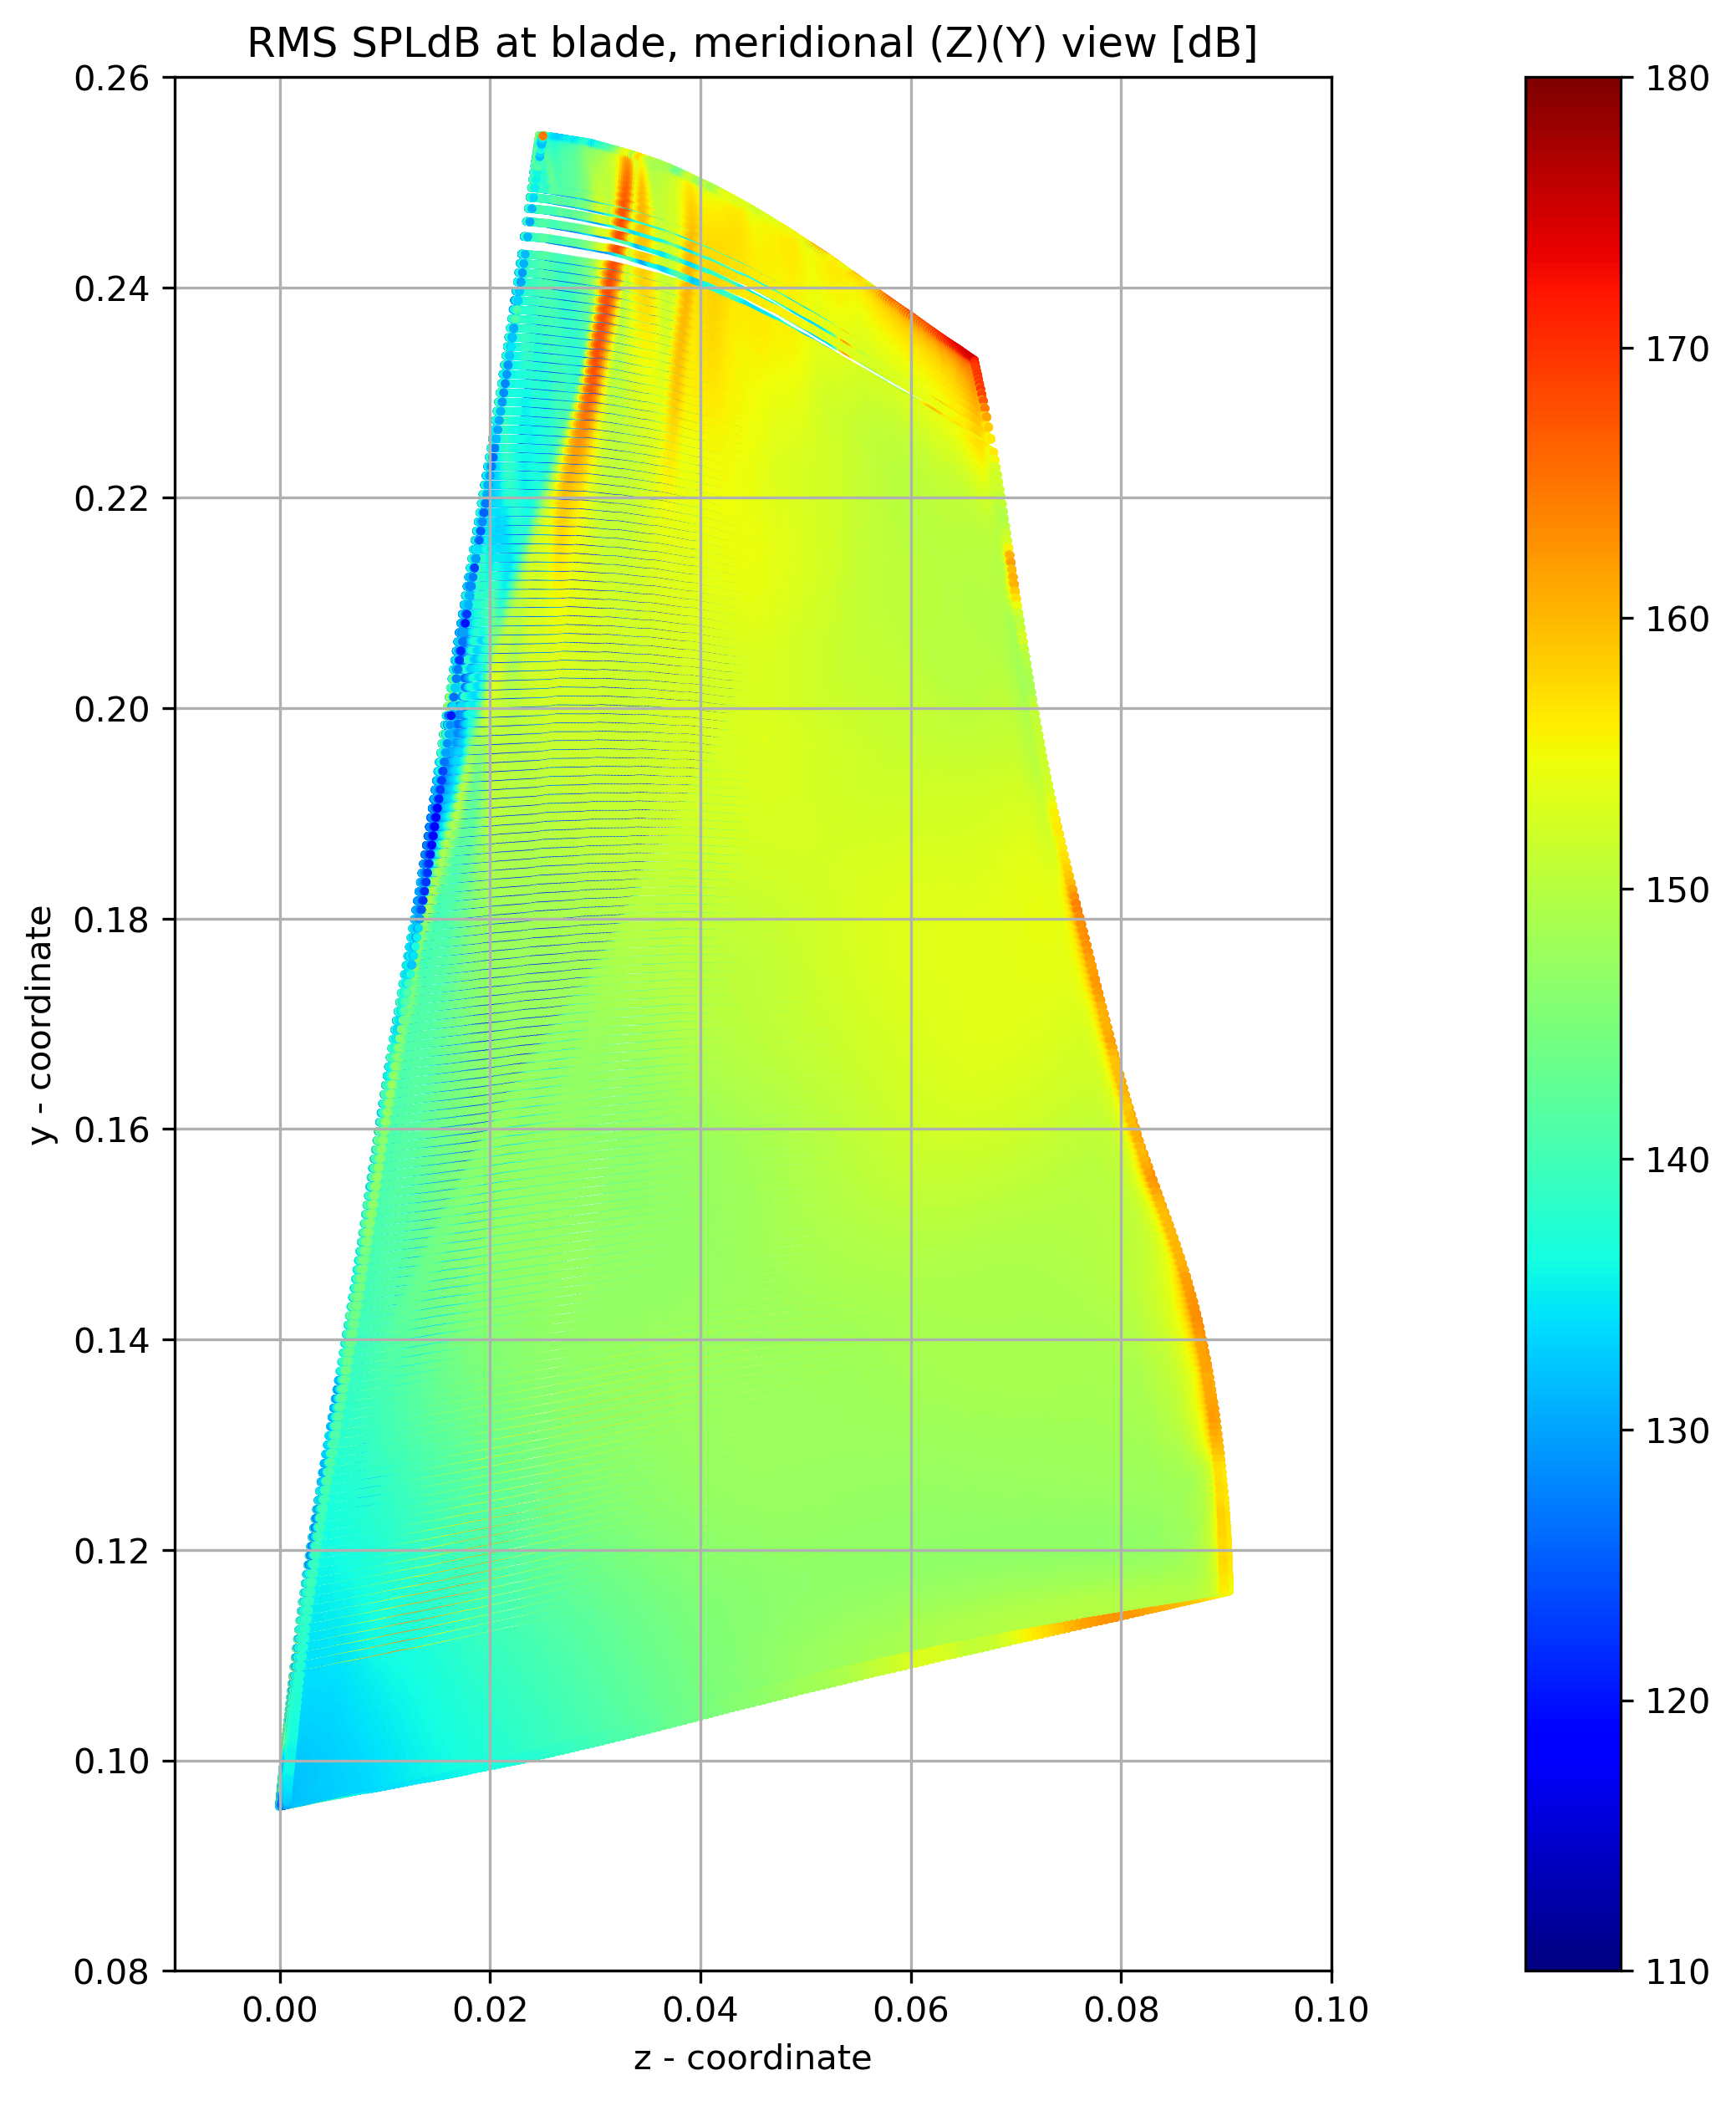
\includegraphics[width=0.85\textwidth]{Figures/blade-zy-rms-spldb.png}
	\caption{RMS SPLdB at blade (zy plane)} \label{blade-zy-rms-spldb}
\end{figure}

\begin{figure}[ht]
	\centering
	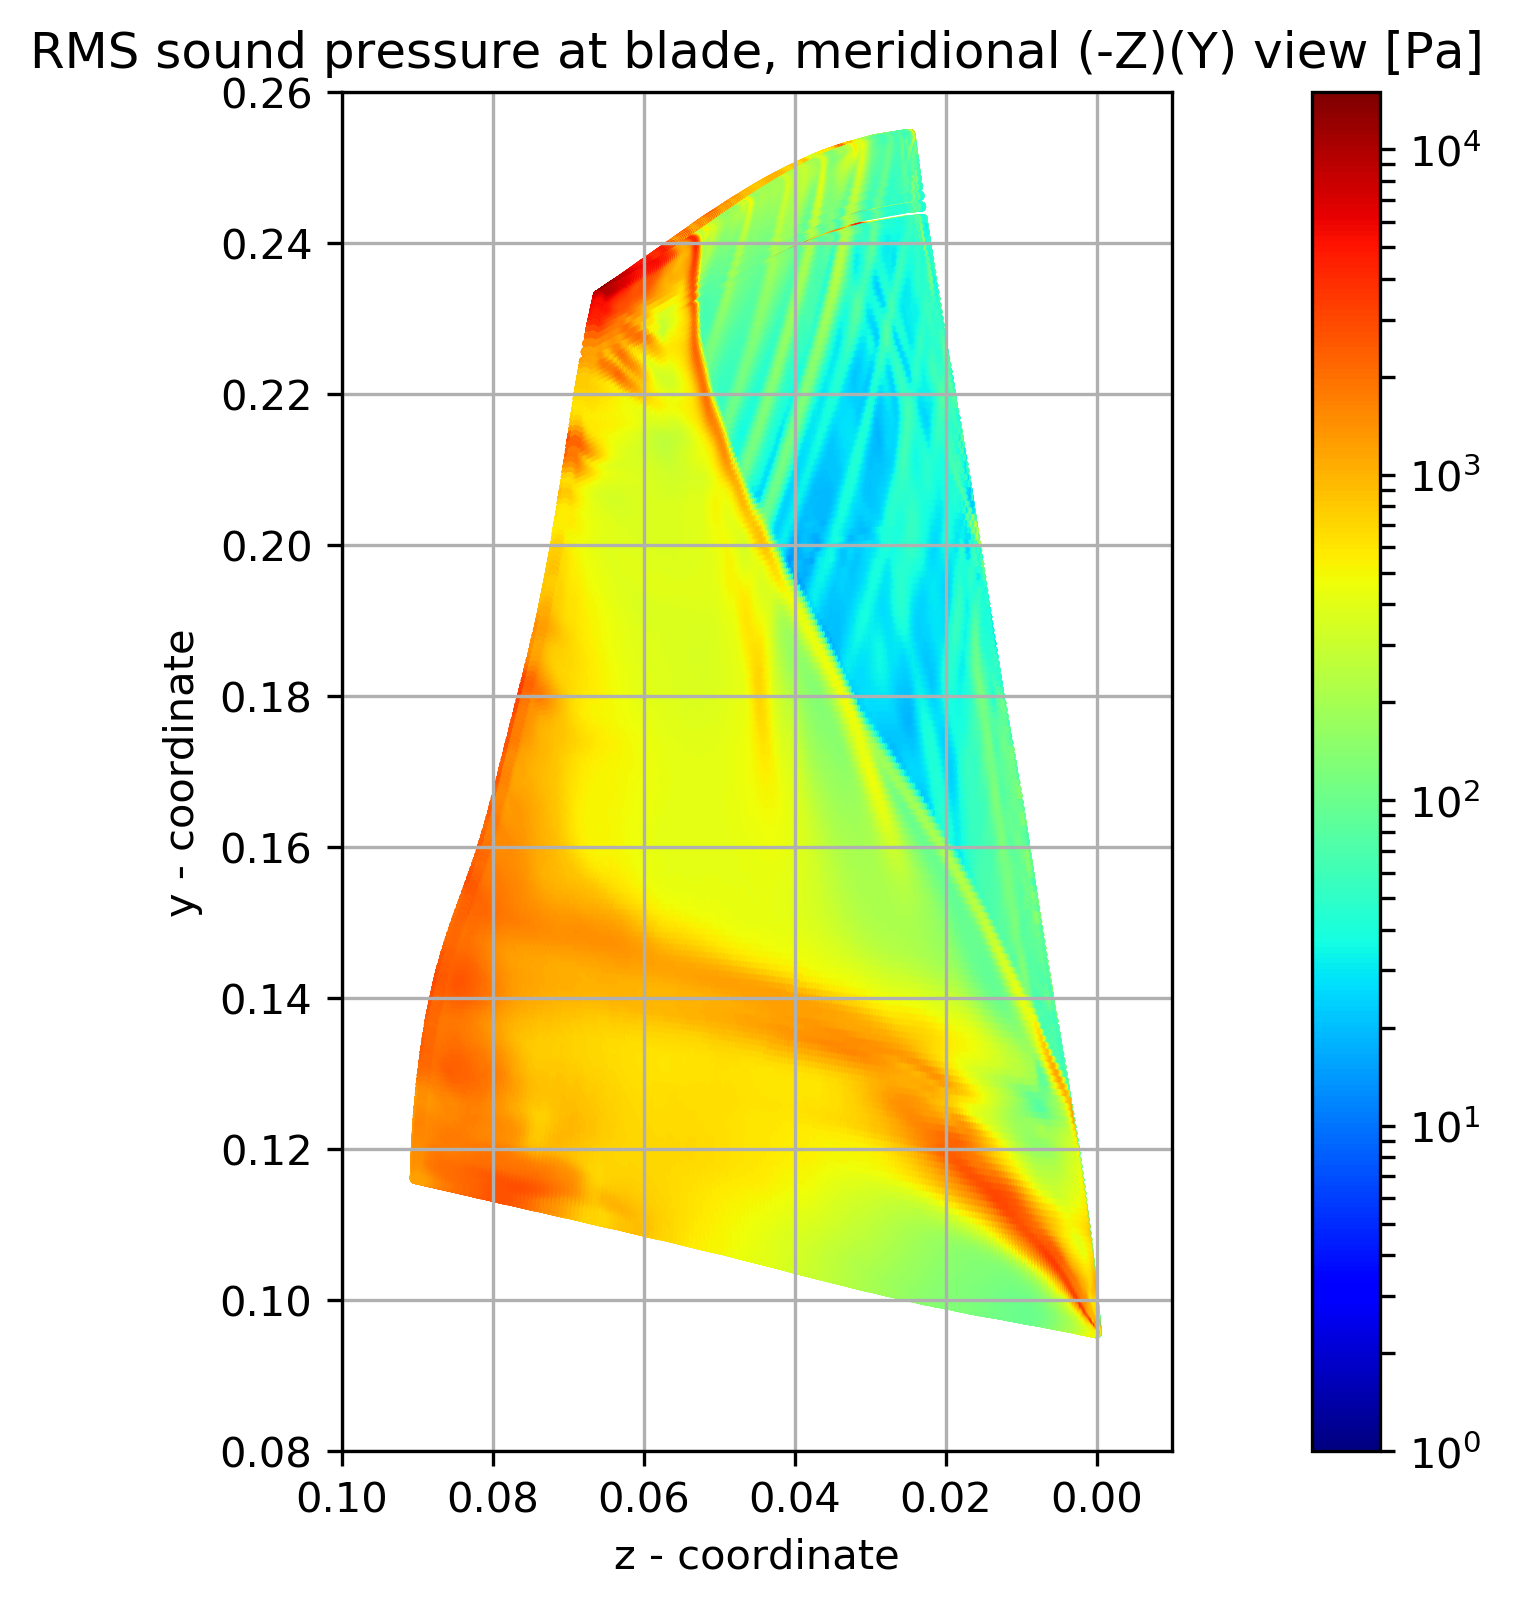
\includegraphics[width=0.85\textwidth]{Figures/blade-negzy-rms-spl.png}
    \caption{RMS Sound pressure at blade (-zy plane)} \label{blade-negzy-rms-spl}
\end{figure}	

\begin{figure}[ht]
	\centering
	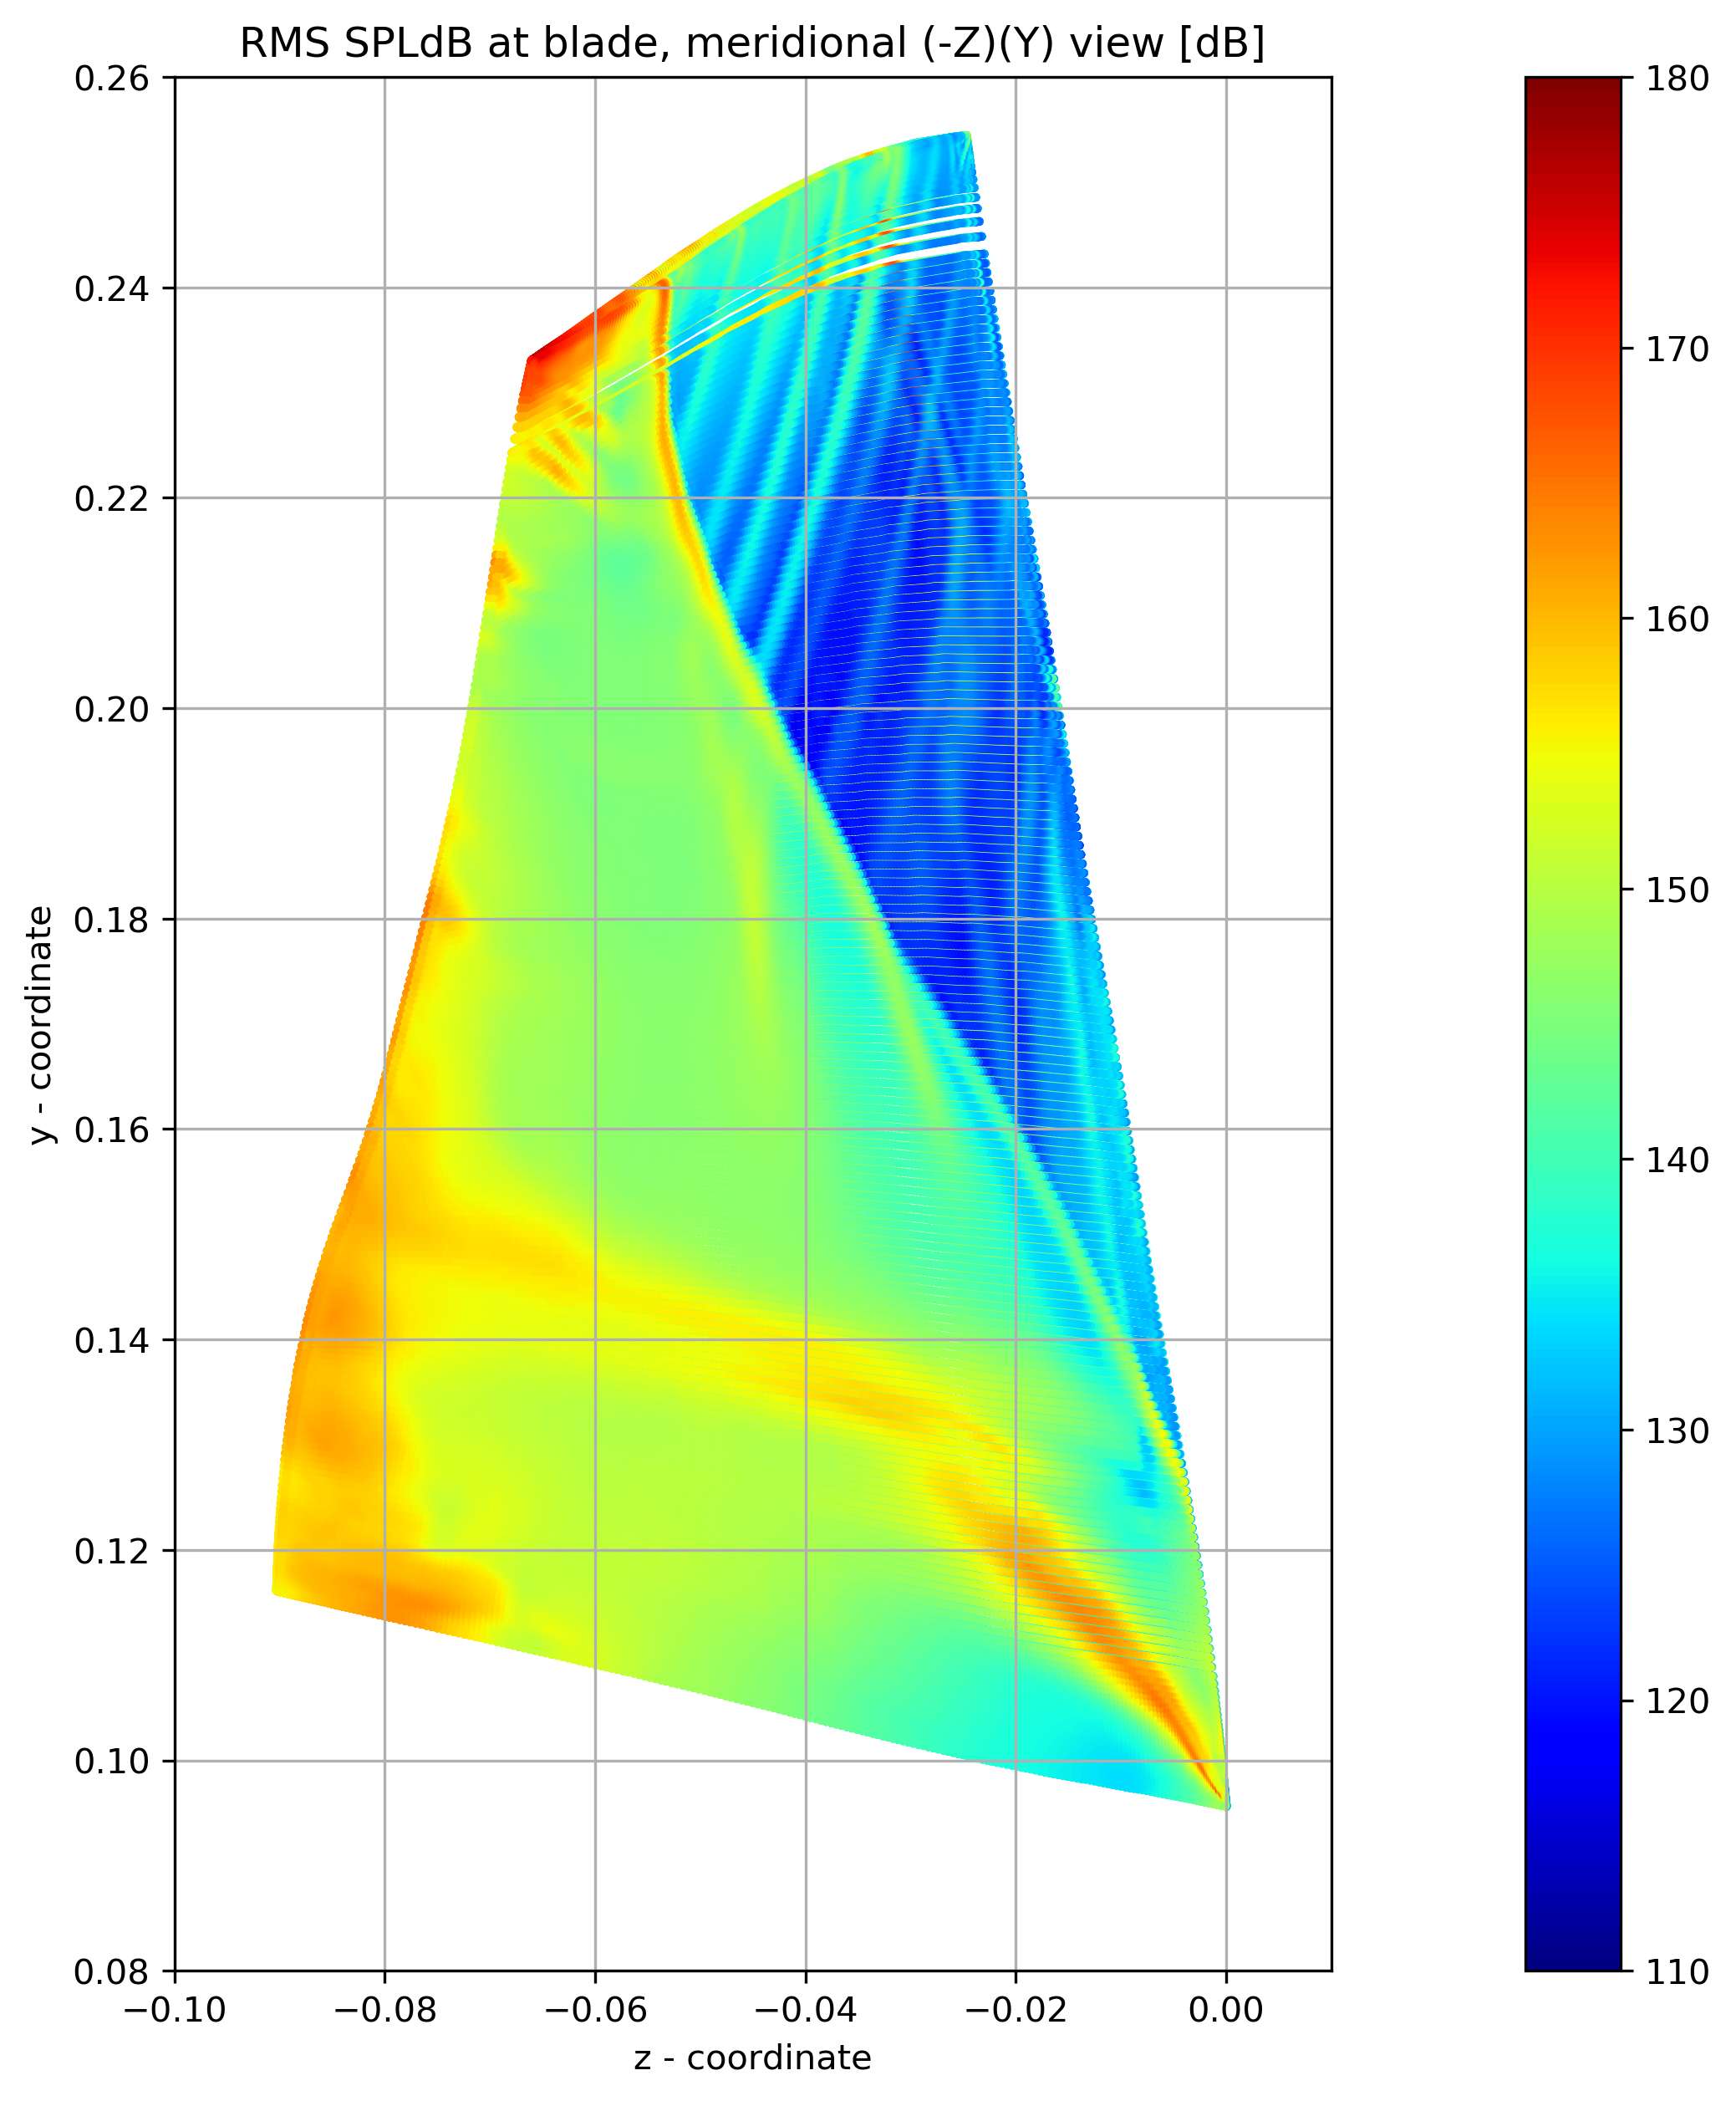
\includegraphics[width=0.85\textwidth]{Figures/blade-negzy-rms-spldb.png}
	\caption{RMS SPLdB at blade (-zy plane)} \label{blade-negzy-rms-spldb}
\end{figure}

\begin{figure}[ht]
	\centering
	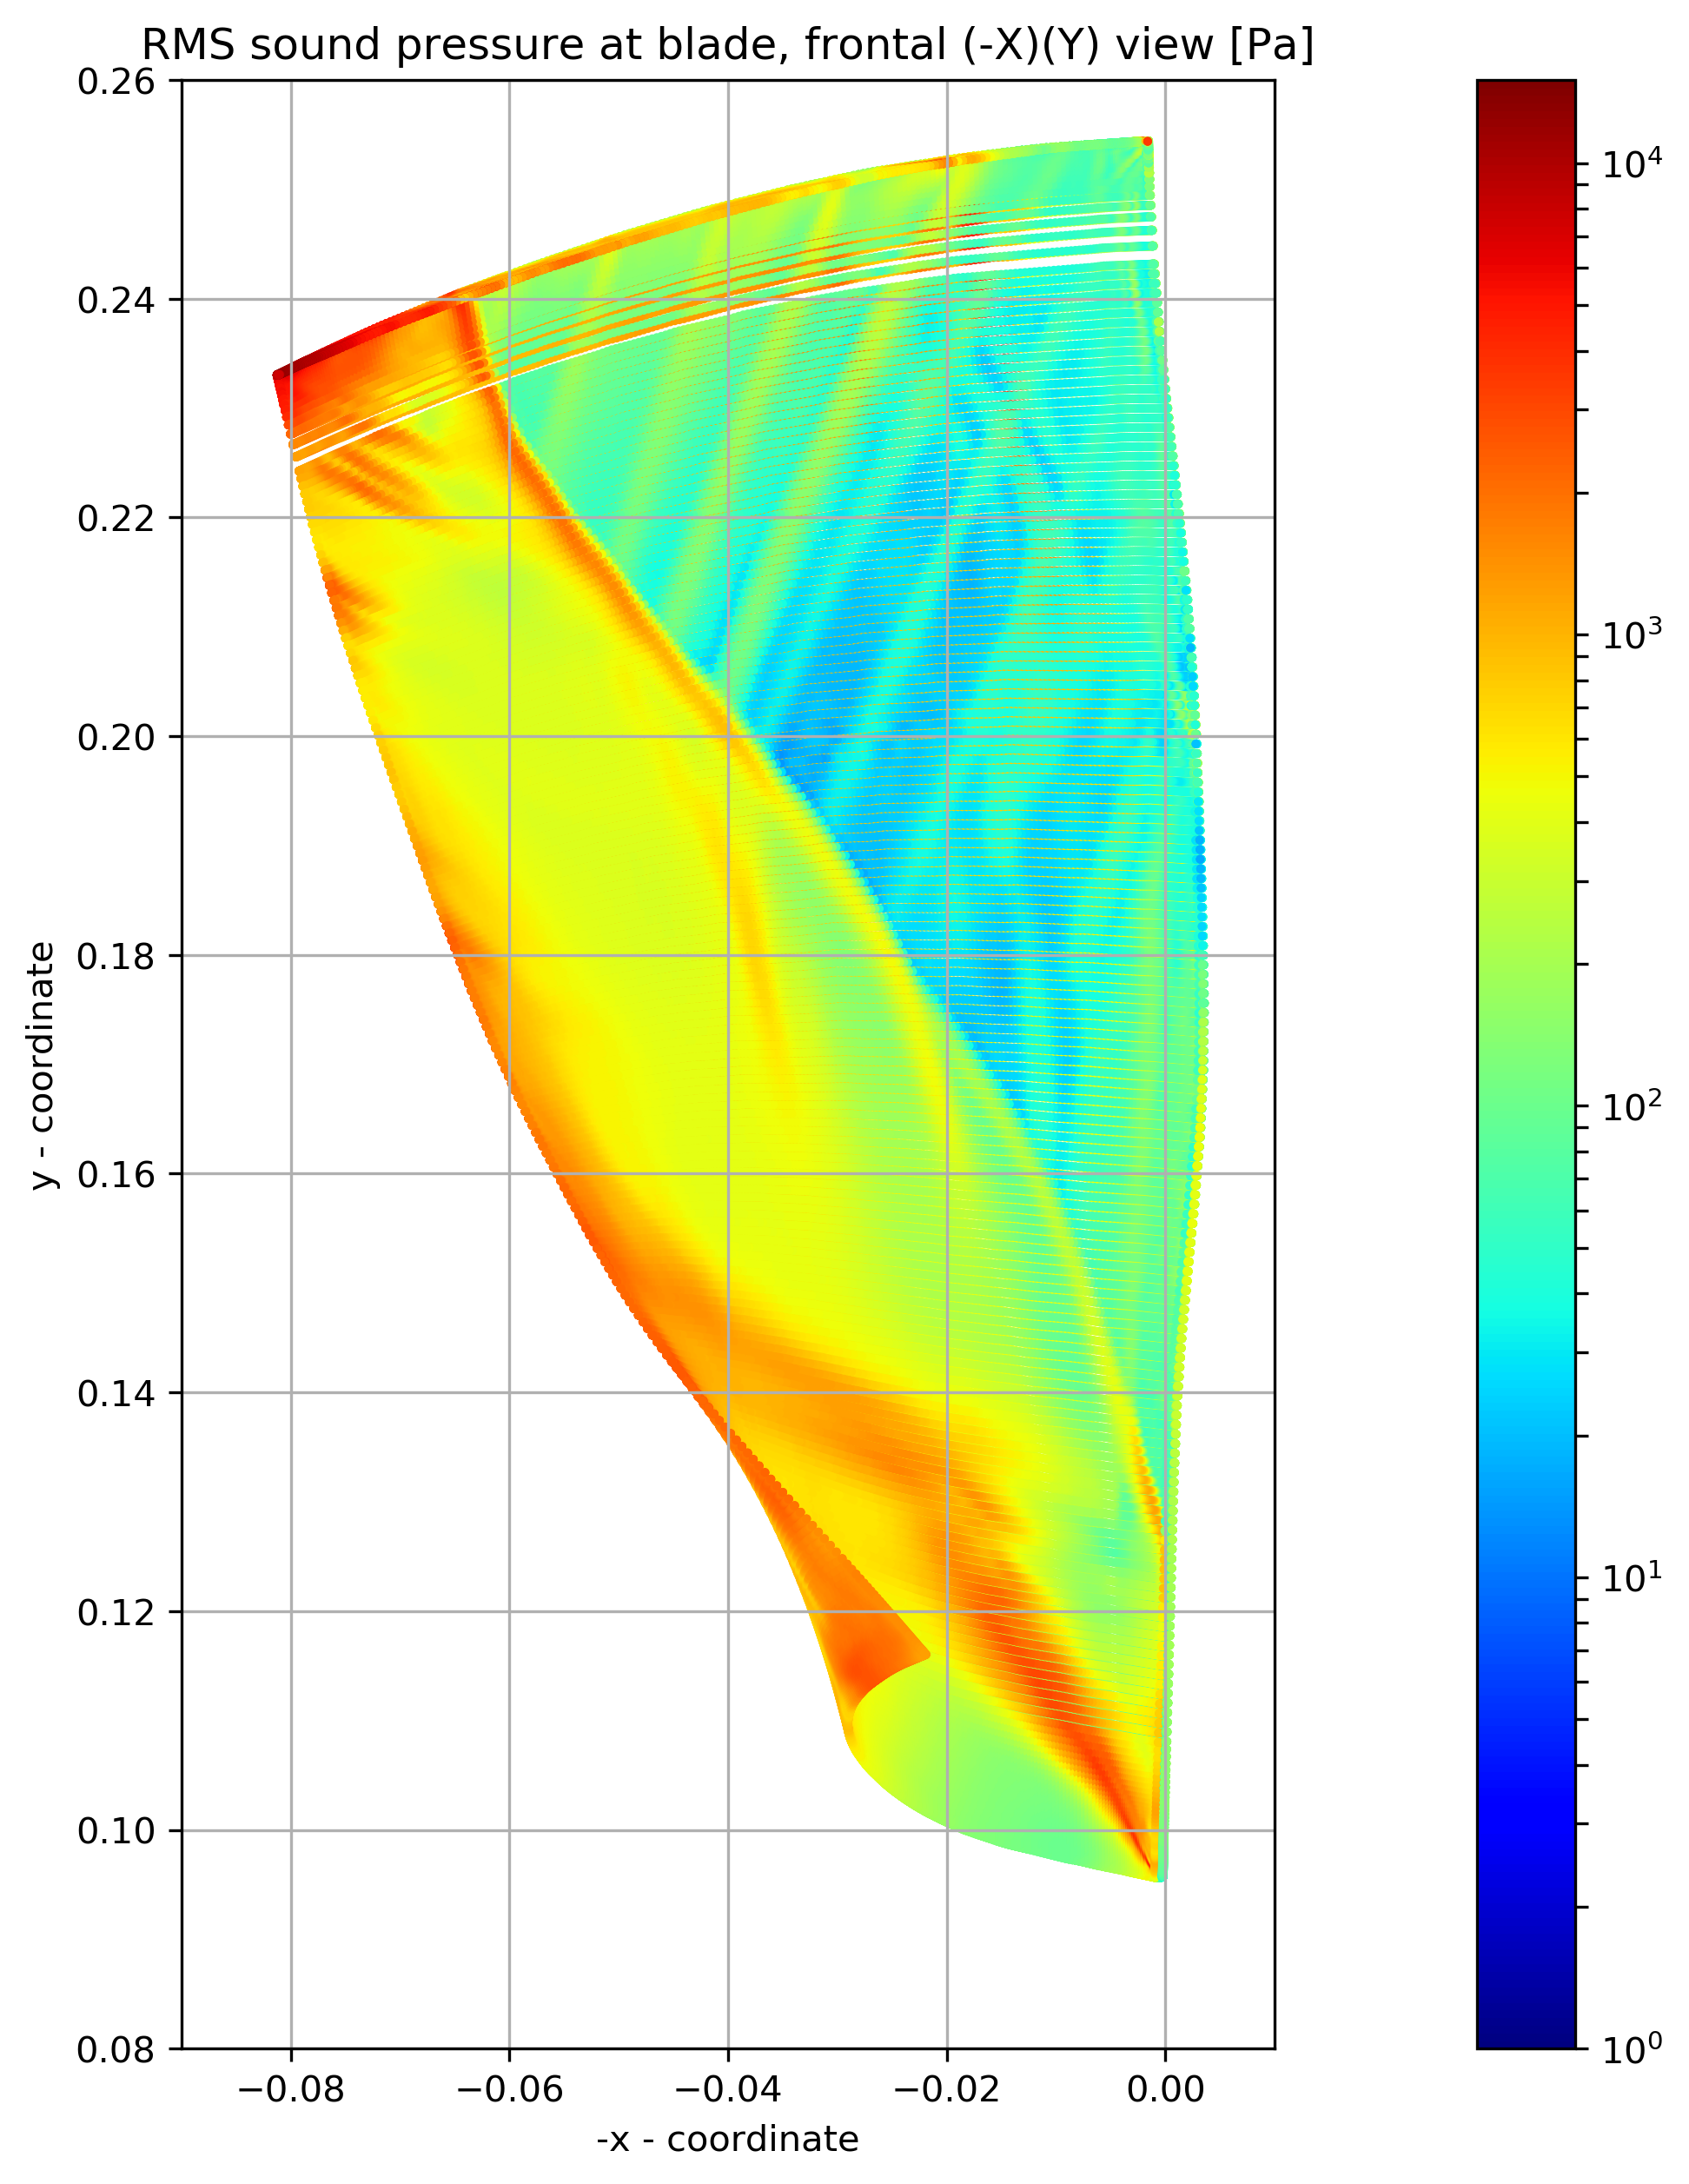
\includegraphics[width=0.85\textwidth]{Figures/blade-negxy-rms-spl.png}
    \caption{RMS Sound pressure at blade (-xy plane)} \label{blade-negxy-rms-spl}
\end{figure}	

\begin{figure}[ht]
	\centering
	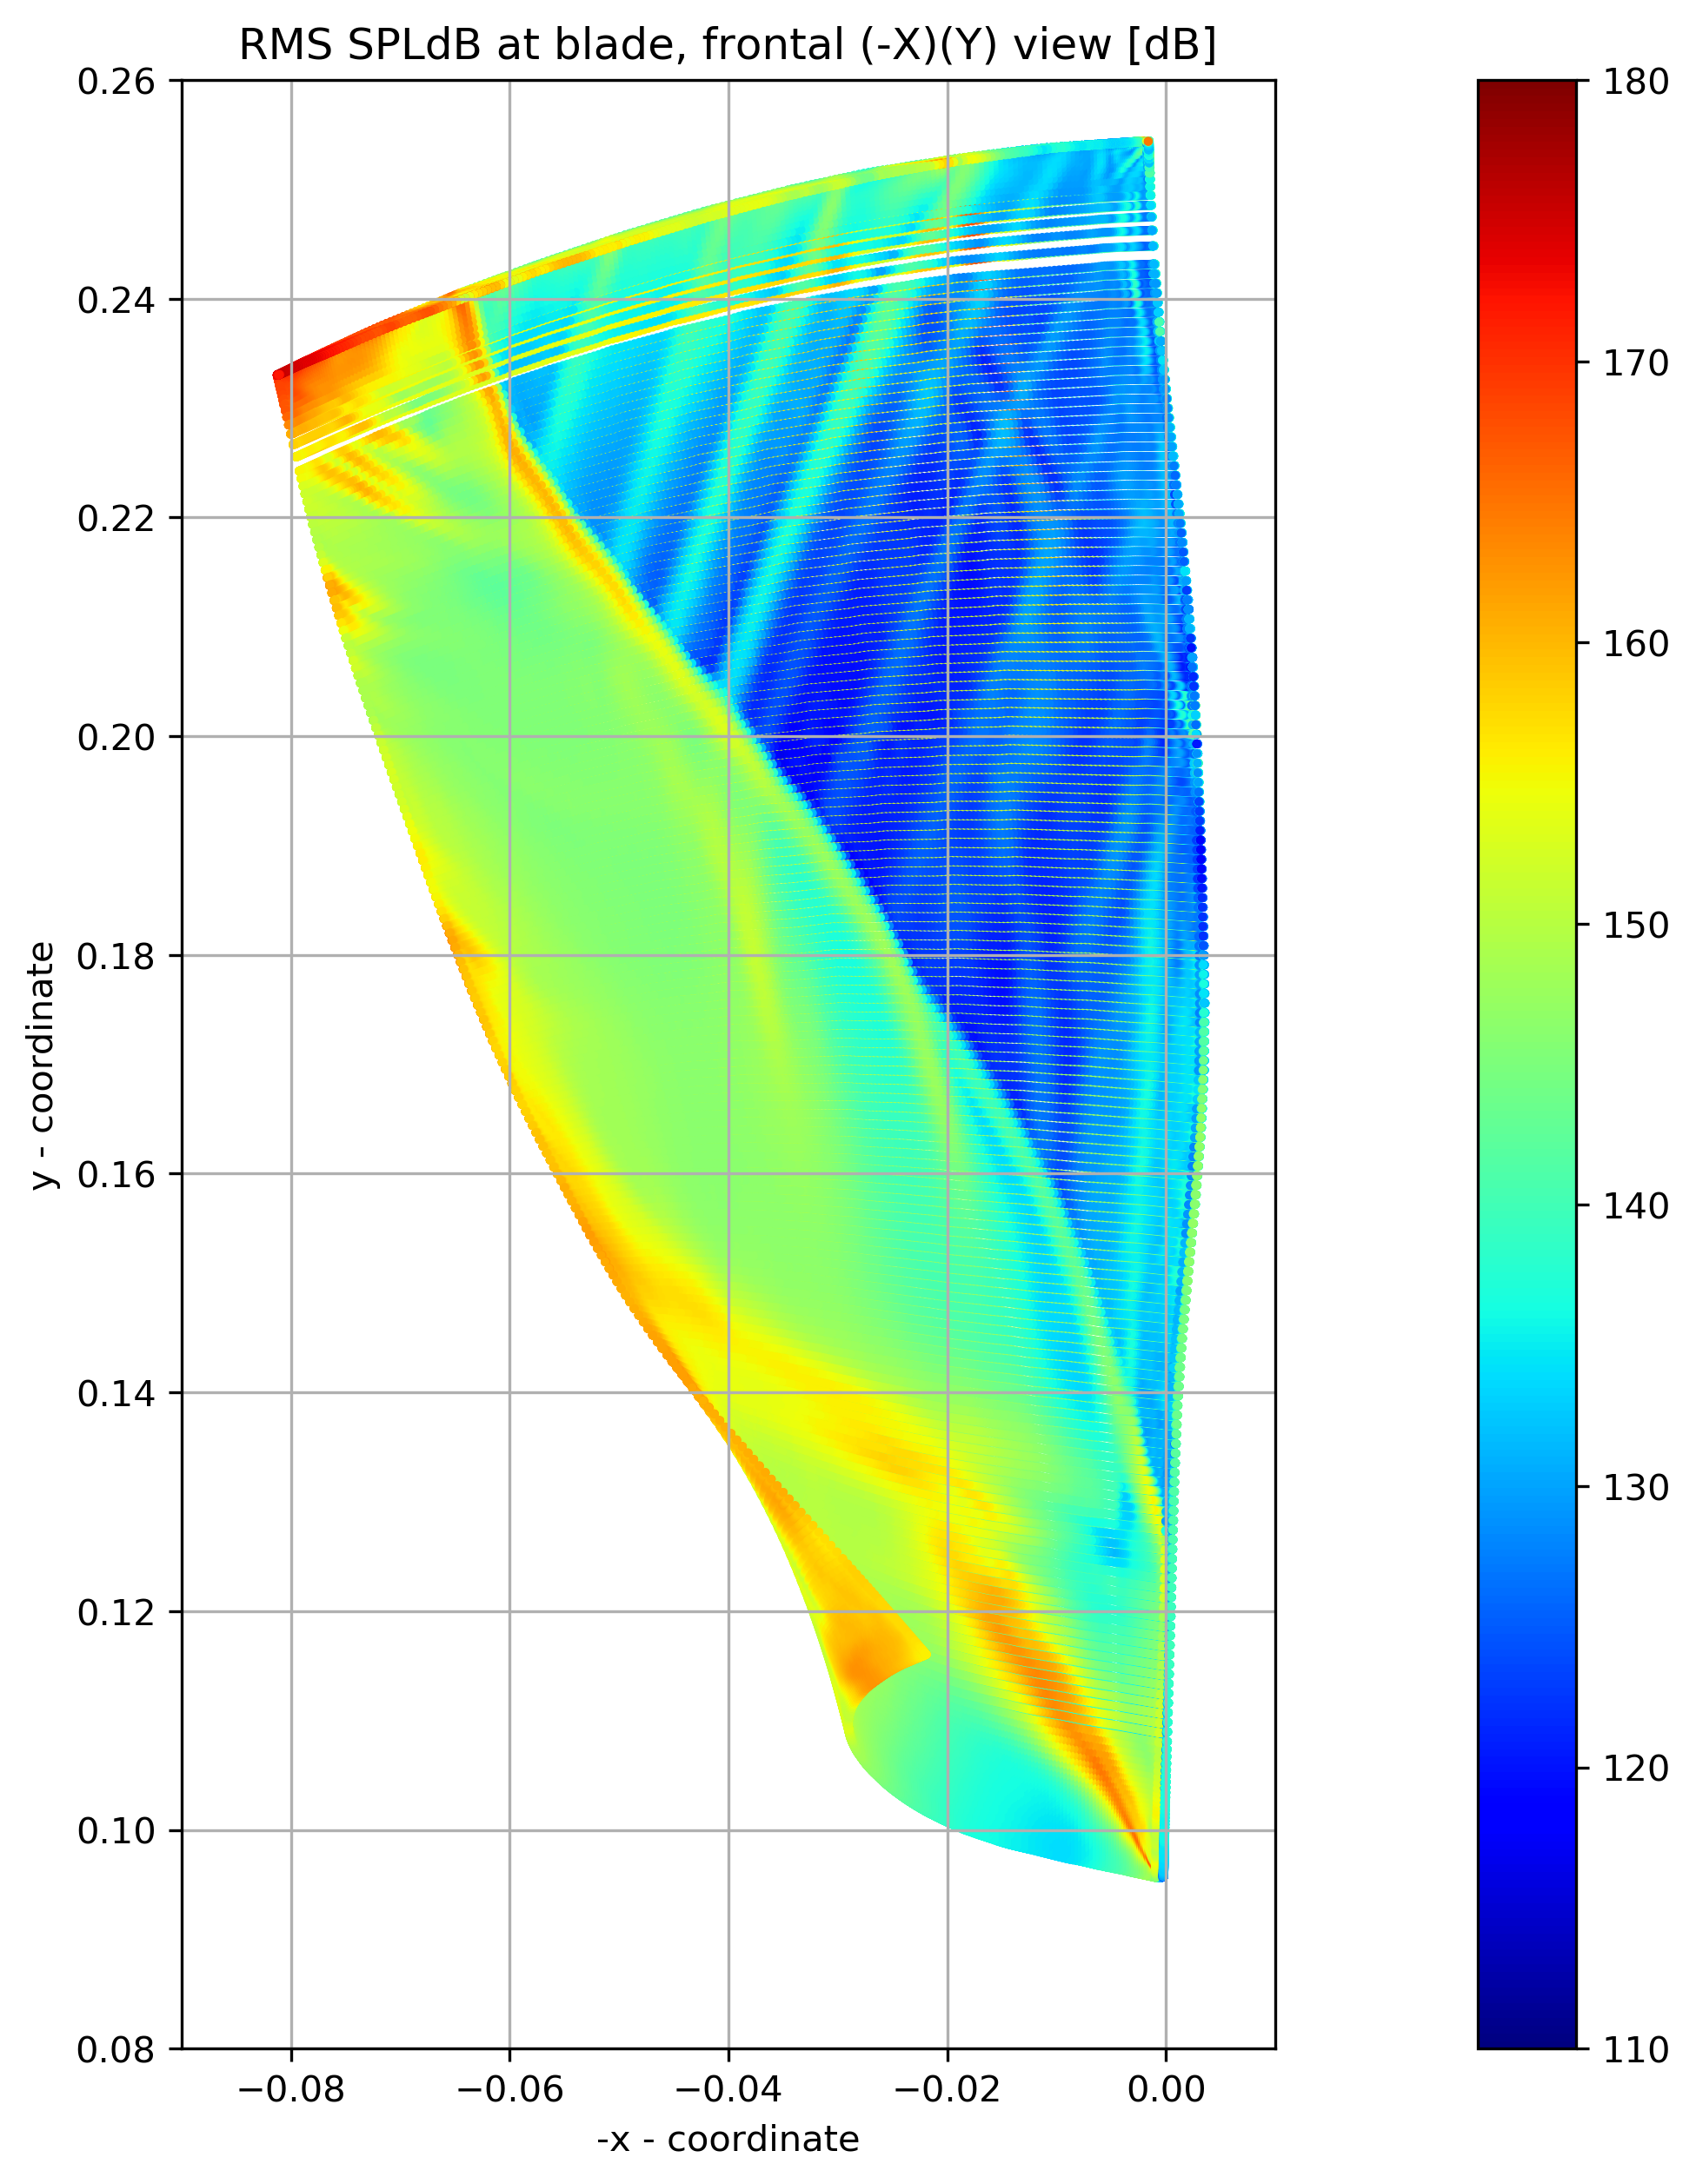
\includegraphics[width=0.85\textwidth]{Figures/blade-negxy-rms-spldb.png}
	\caption{RMS SPLdB at blade (-xy plane)} \label{blade-negxy-rms-spldb}
\end{figure}

\begin{figure}[ht]
	\centering
	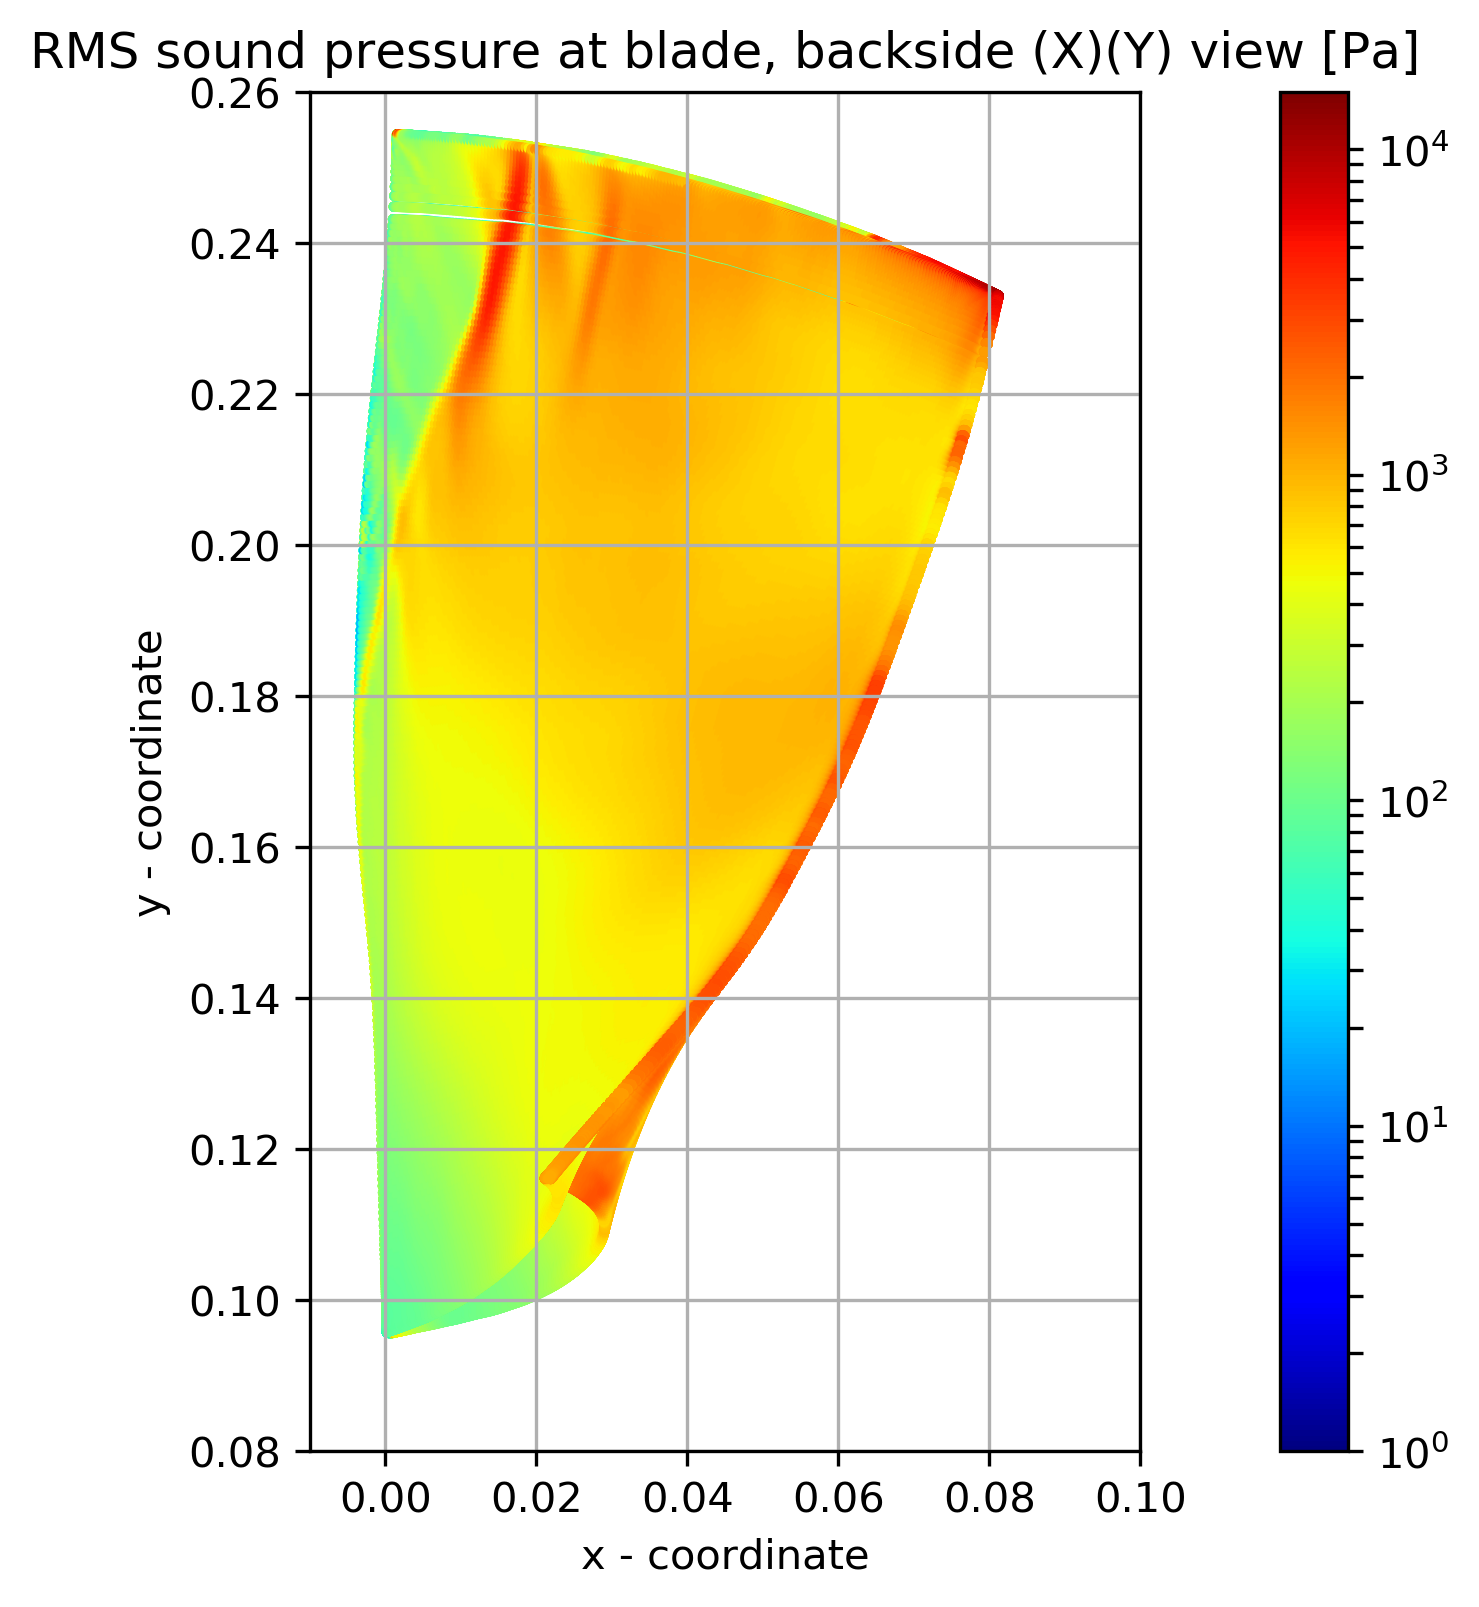
\includegraphics[width=0.85\textwidth]{Figures/blade-xy-rms-spl.png}
    \caption{RMS Sound pressure at blade (xy plane)} \label{blade-xy-rms-spl}
\end{figure}	

\begin{figure}[ht]
	\centering
	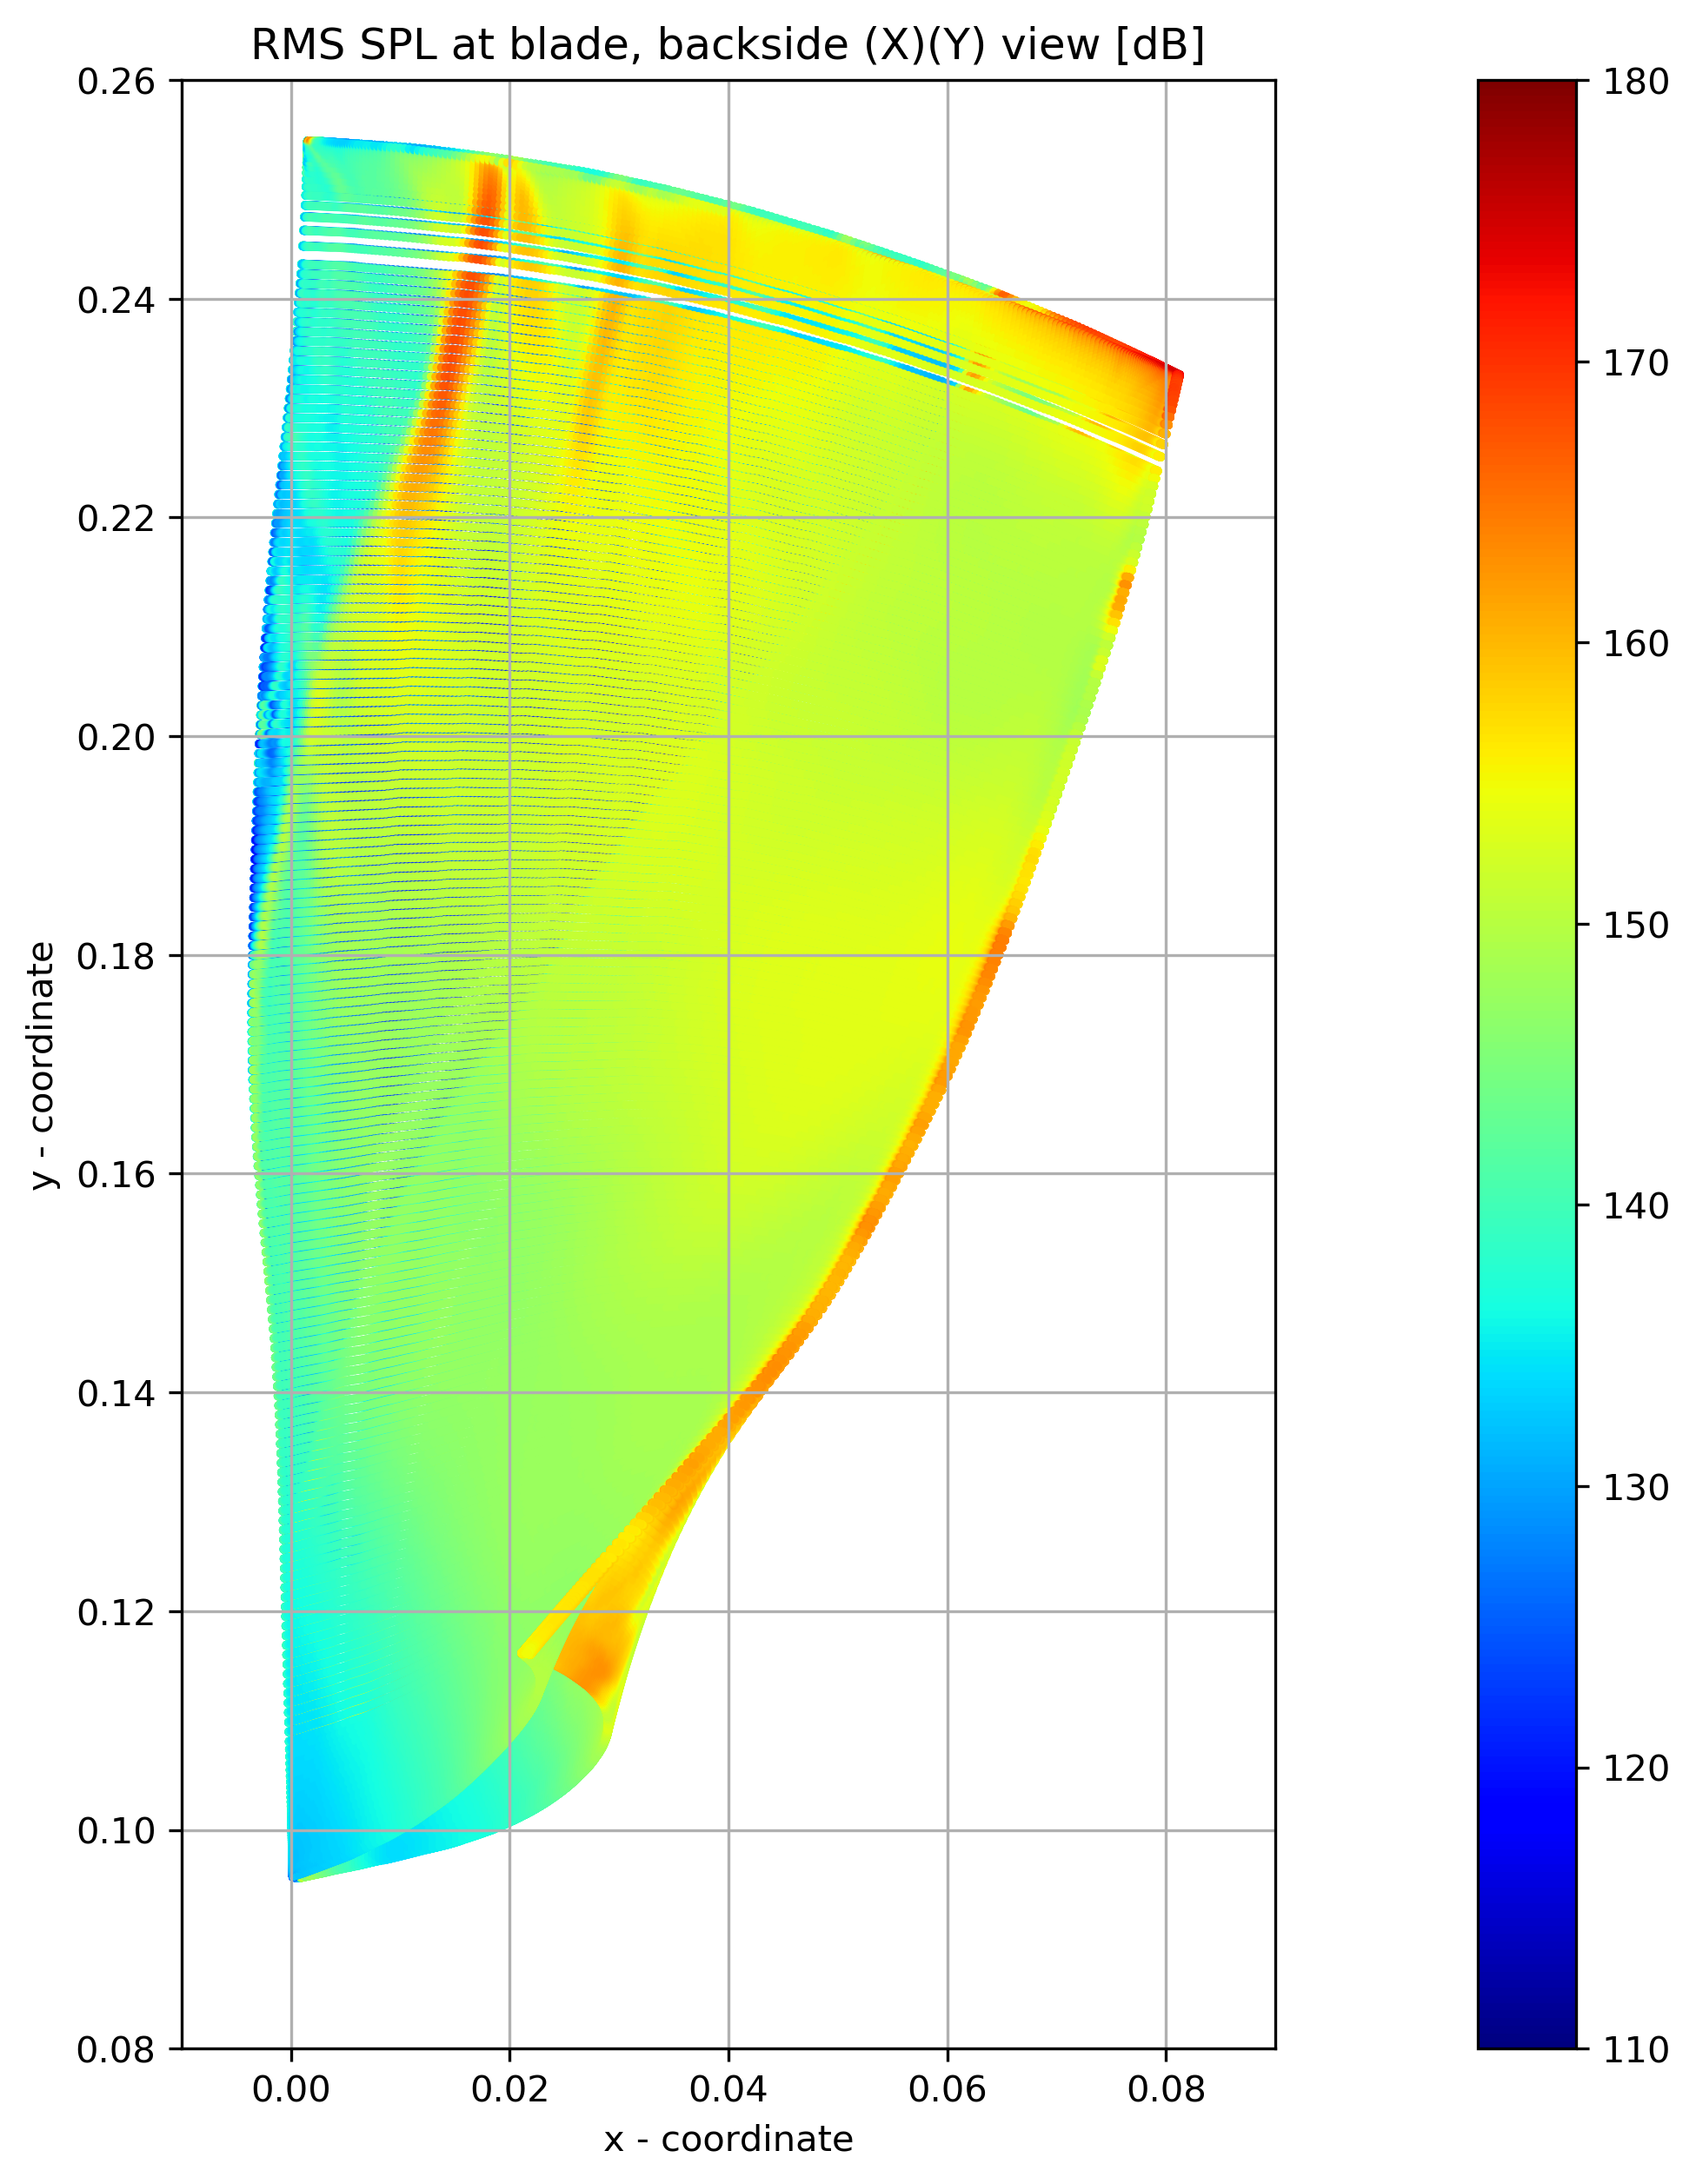
\includegraphics[width=0.85\textwidth]{Figures/blade-xy-rms-spldb.png}
	\caption{RMS SPLdB at blade (xy plane)} \label{blade-xy-rms-spldb}
\end{figure}

%int-01
\begin{figure}[ht]
  \centering
  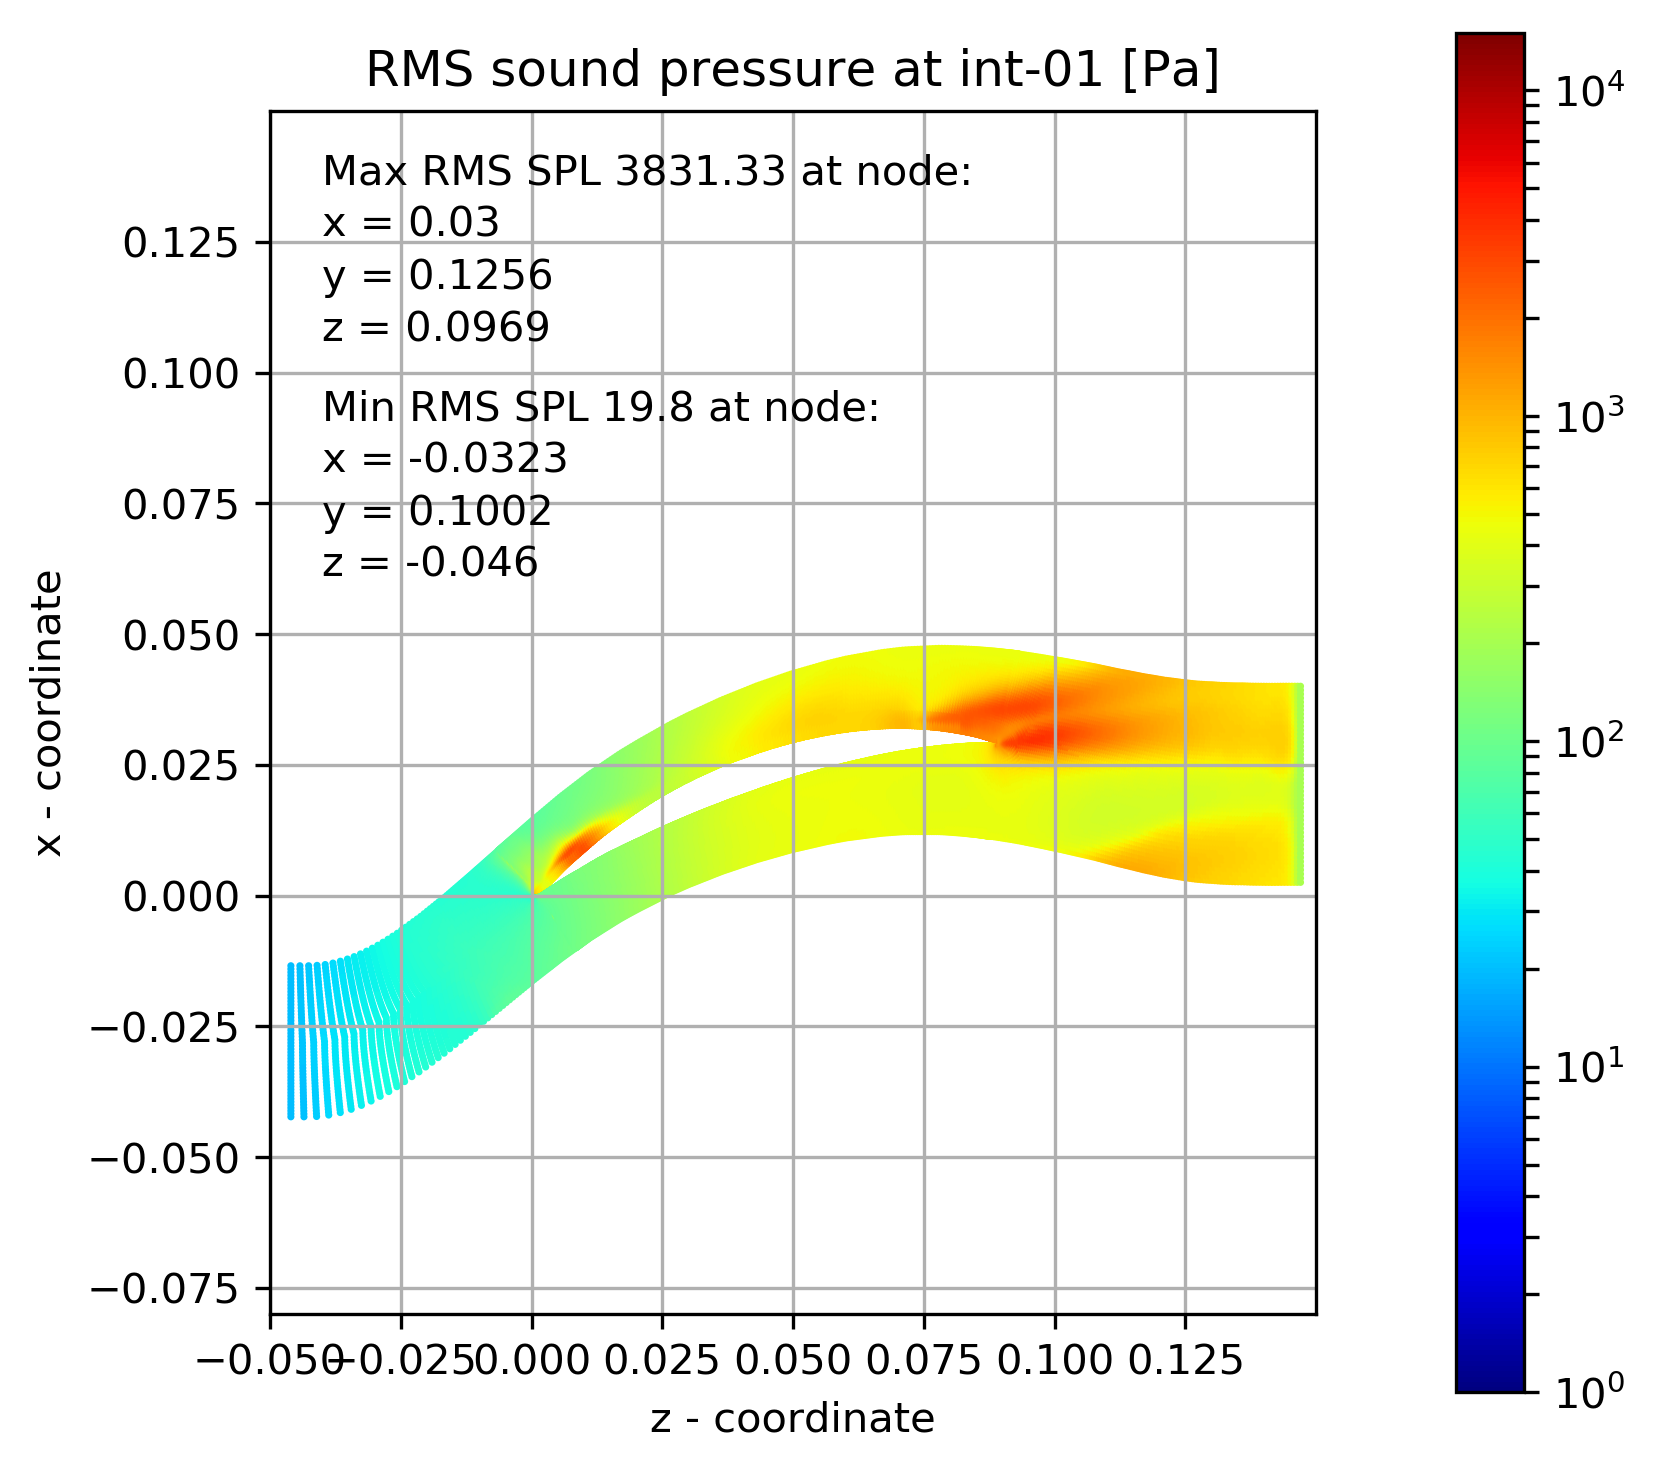
\includegraphics[width=0.75\textwidth]{Figures/int-01-rms-spl.png}
  \caption{RMS Sound pressure at int-01 mark} \label{int-01-rms-spl}
  
  \vspace*{\floatsep}% https://tex.stackexchange.com/q/26521/5764

  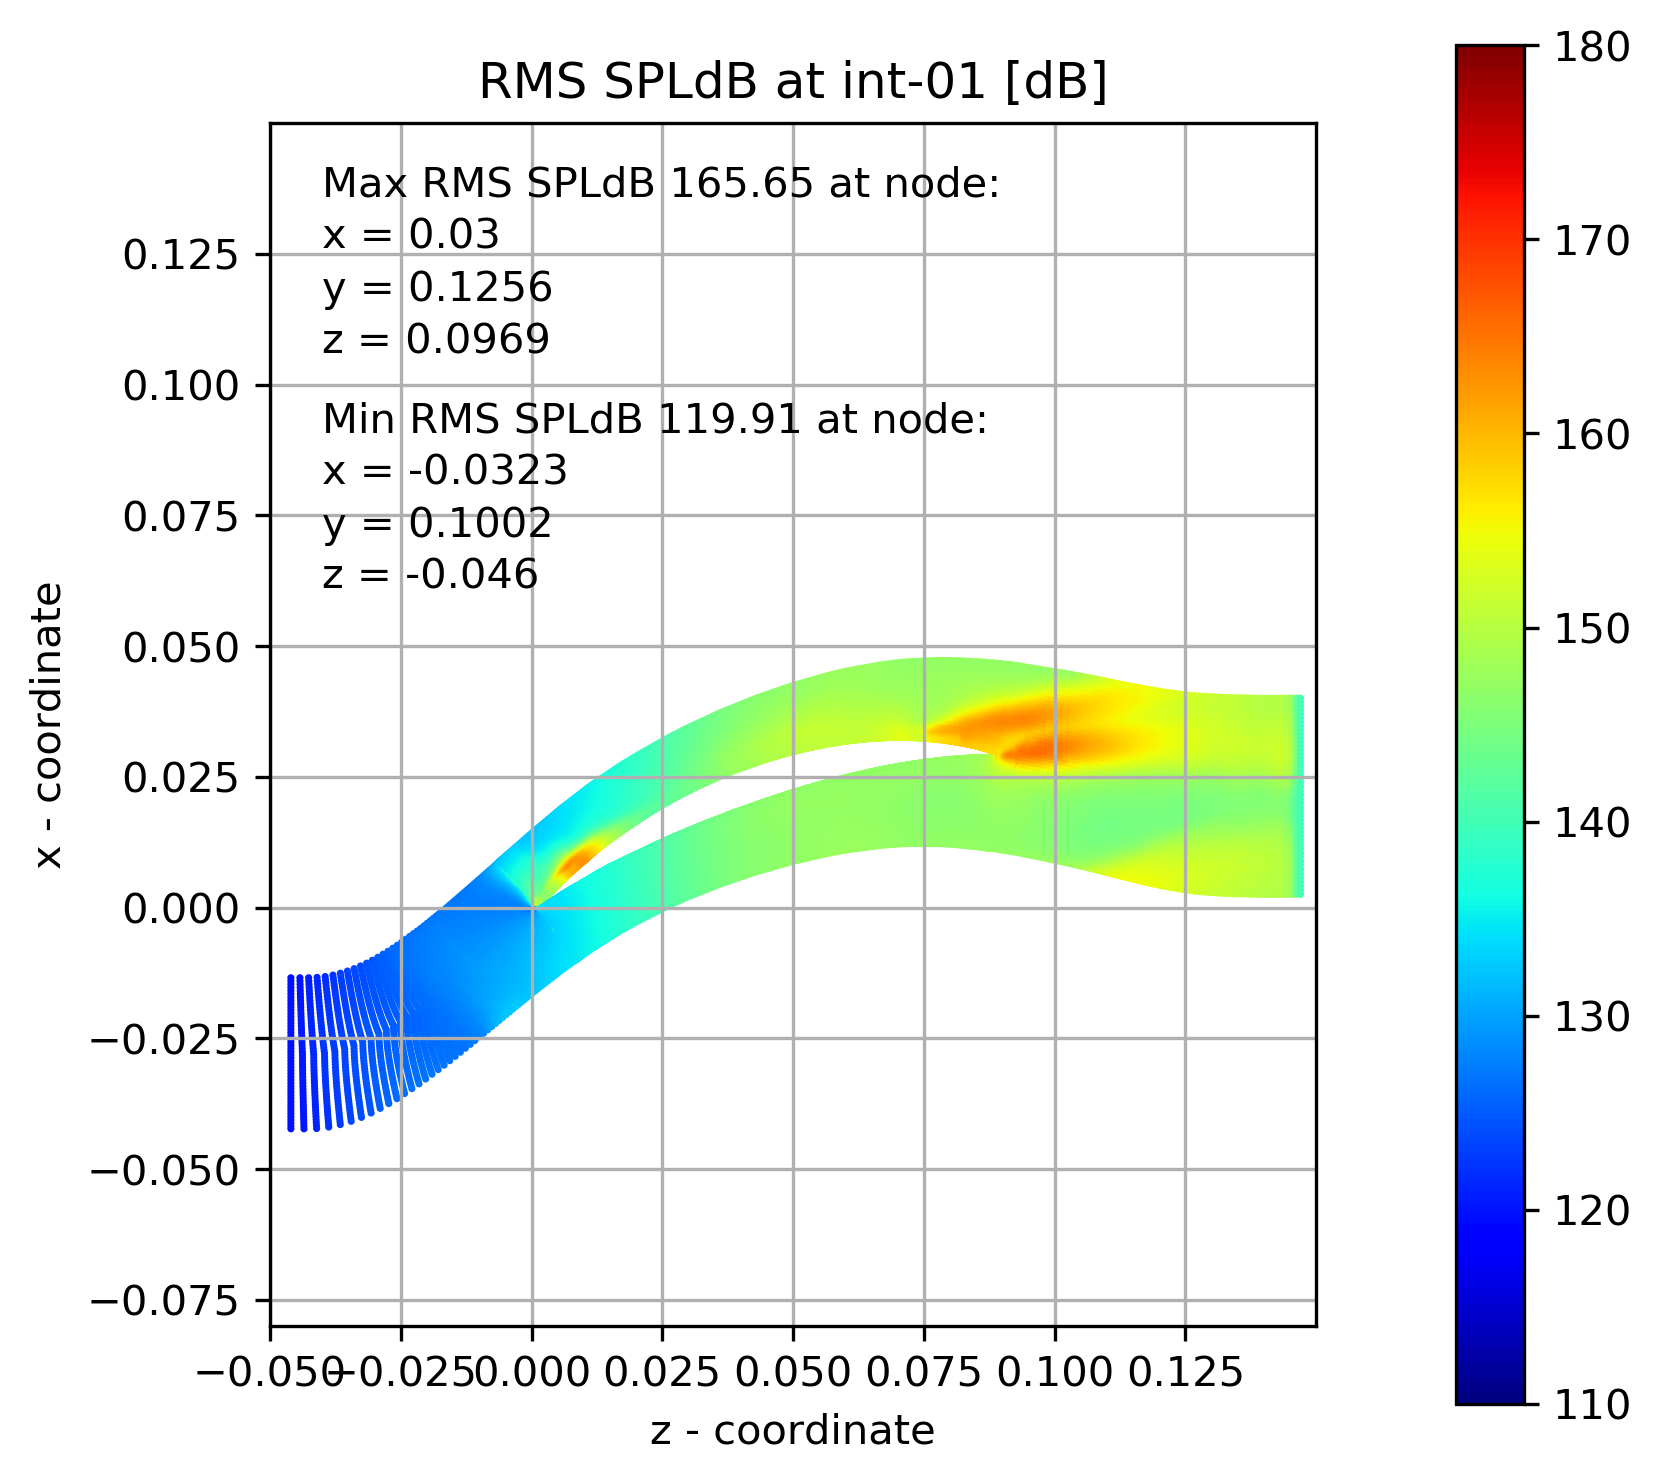
\includegraphics[width=0.75\textwidth]{Figures/int-01-rms-spldb.png}
  \caption{RMS Sound pressure decibel level at int-01 mark} \label{int-01-rms-spldb}
\end{figure}
%int-01
\begin{figure}[ht]
  \centering
  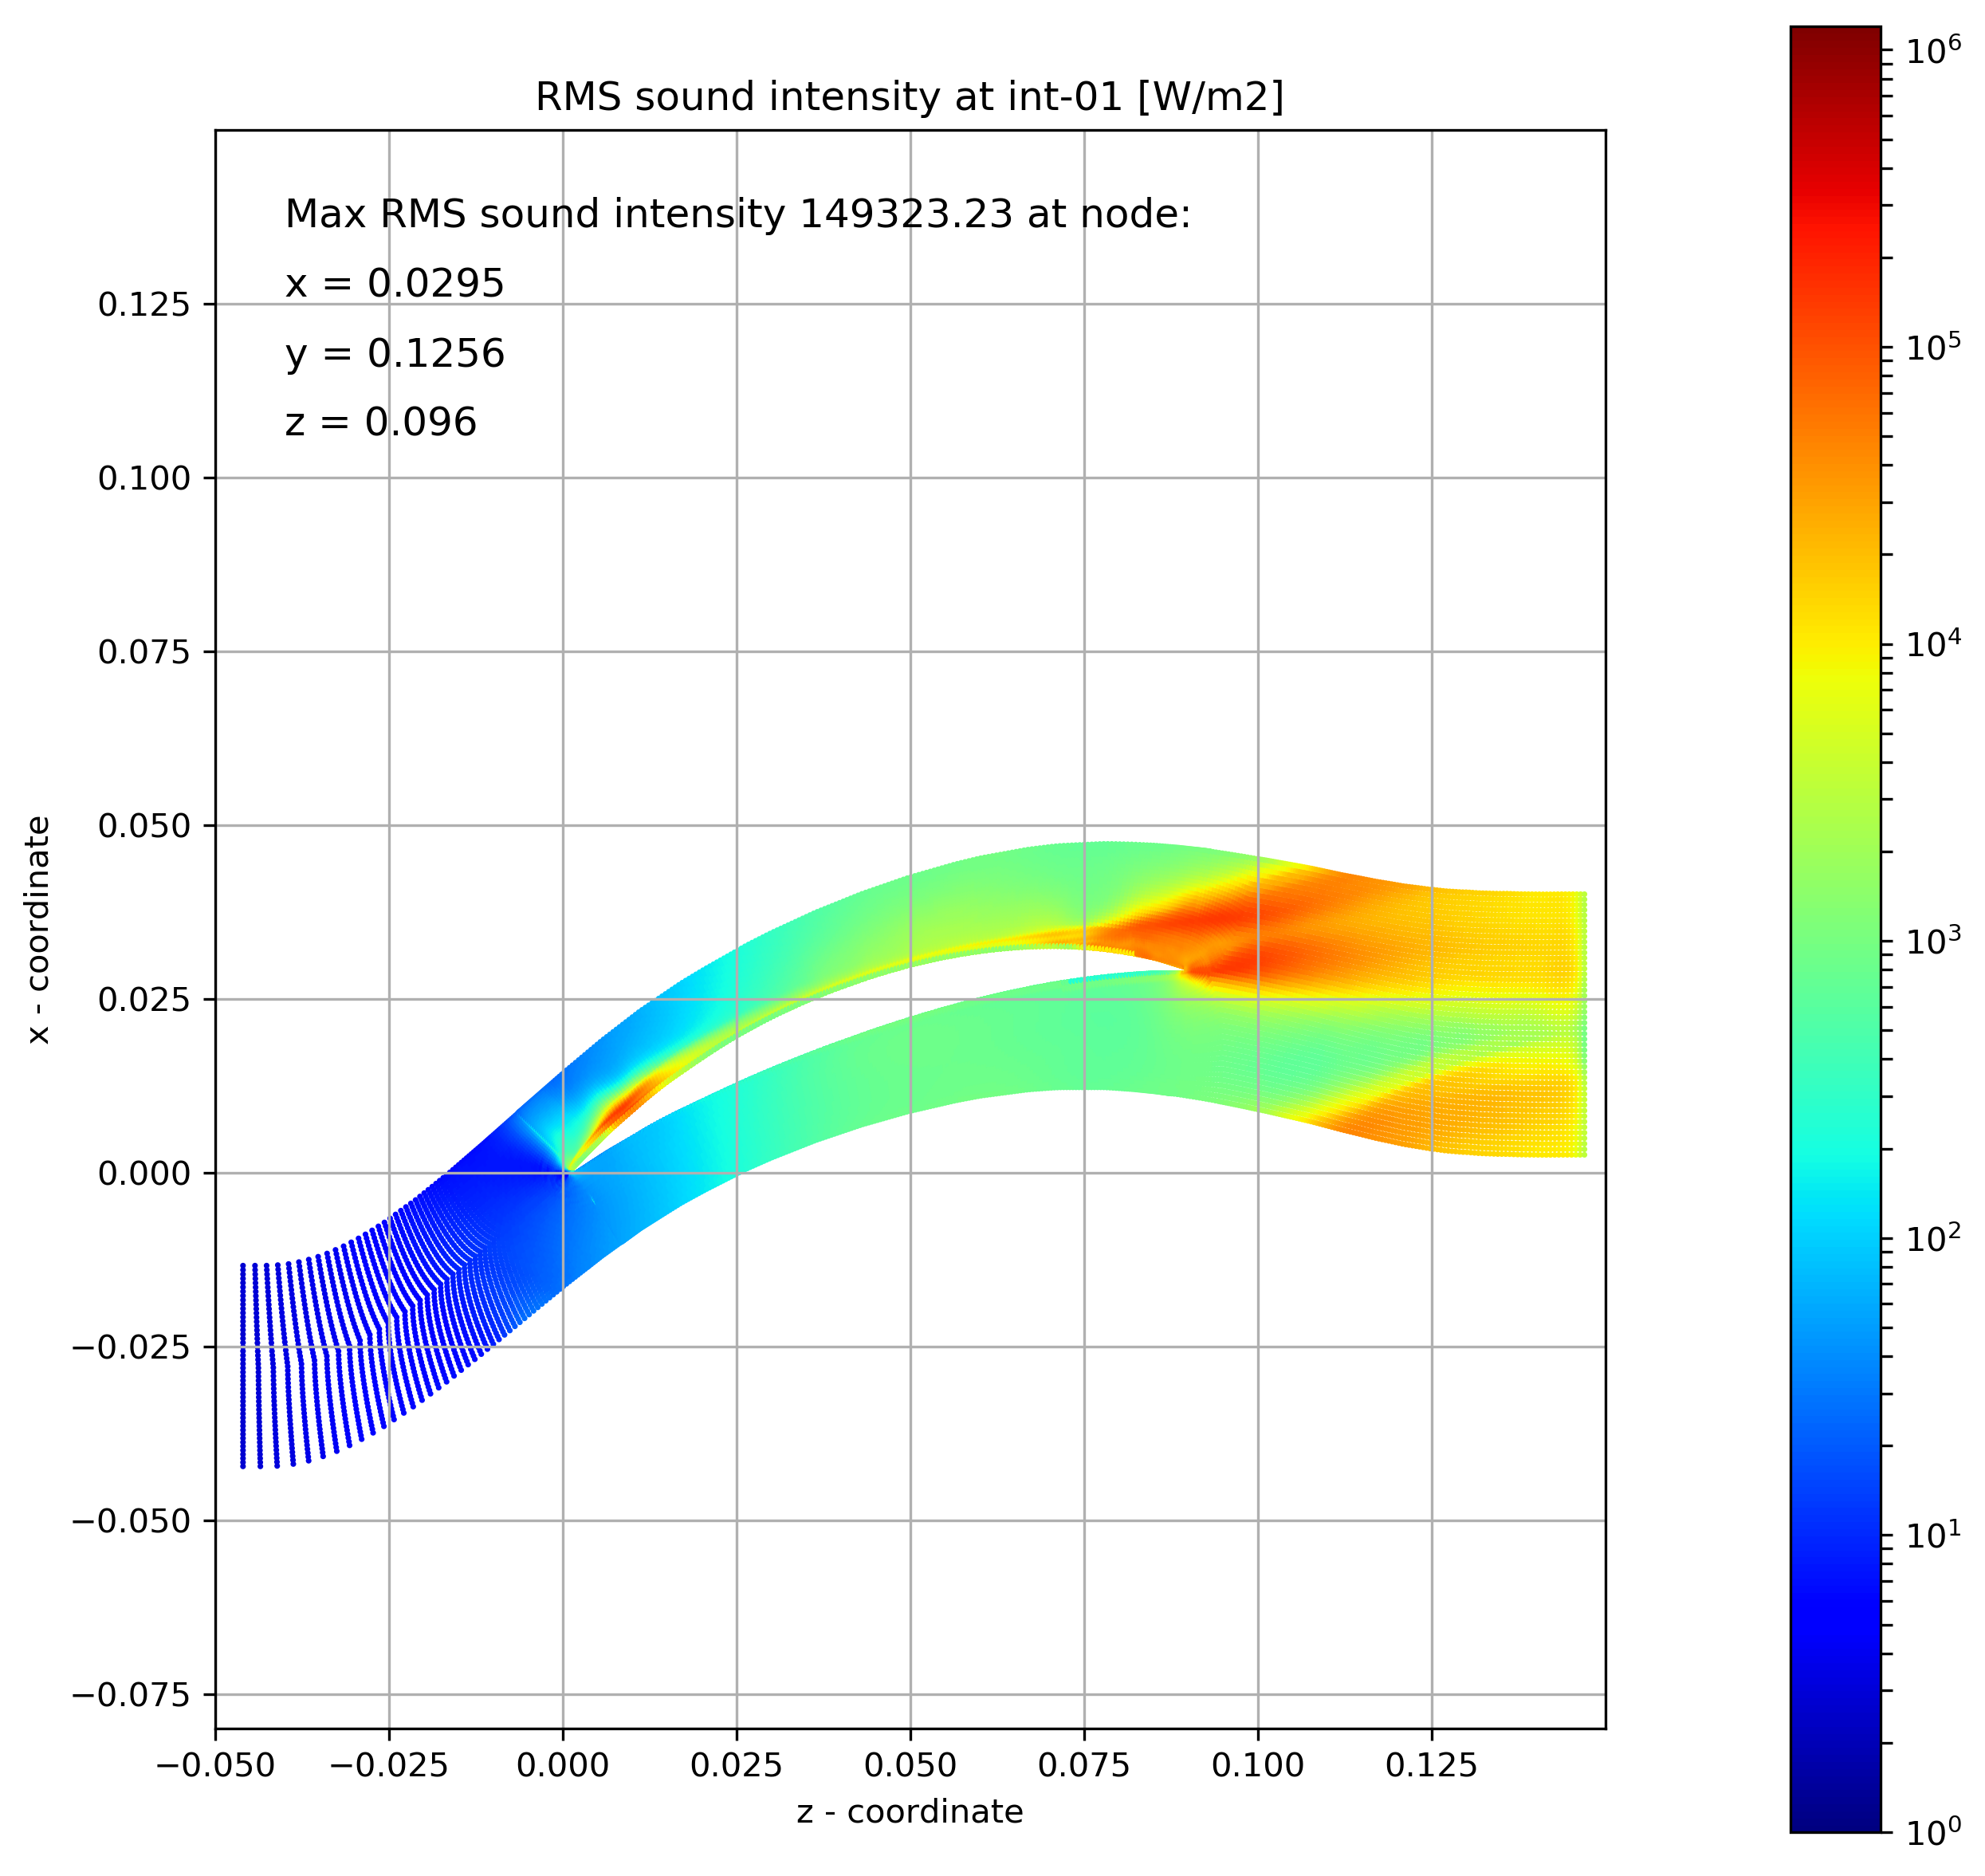
\includegraphics[width=0.75\textwidth]{Figures/int-01-rms-sil.png}
  \caption{RMS Sound intensity at int-01 mark} \label{int-01-rms-sil}
  
  \vspace*{\floatsep}% https://tex.stackexchange.com/q/26521/5764

  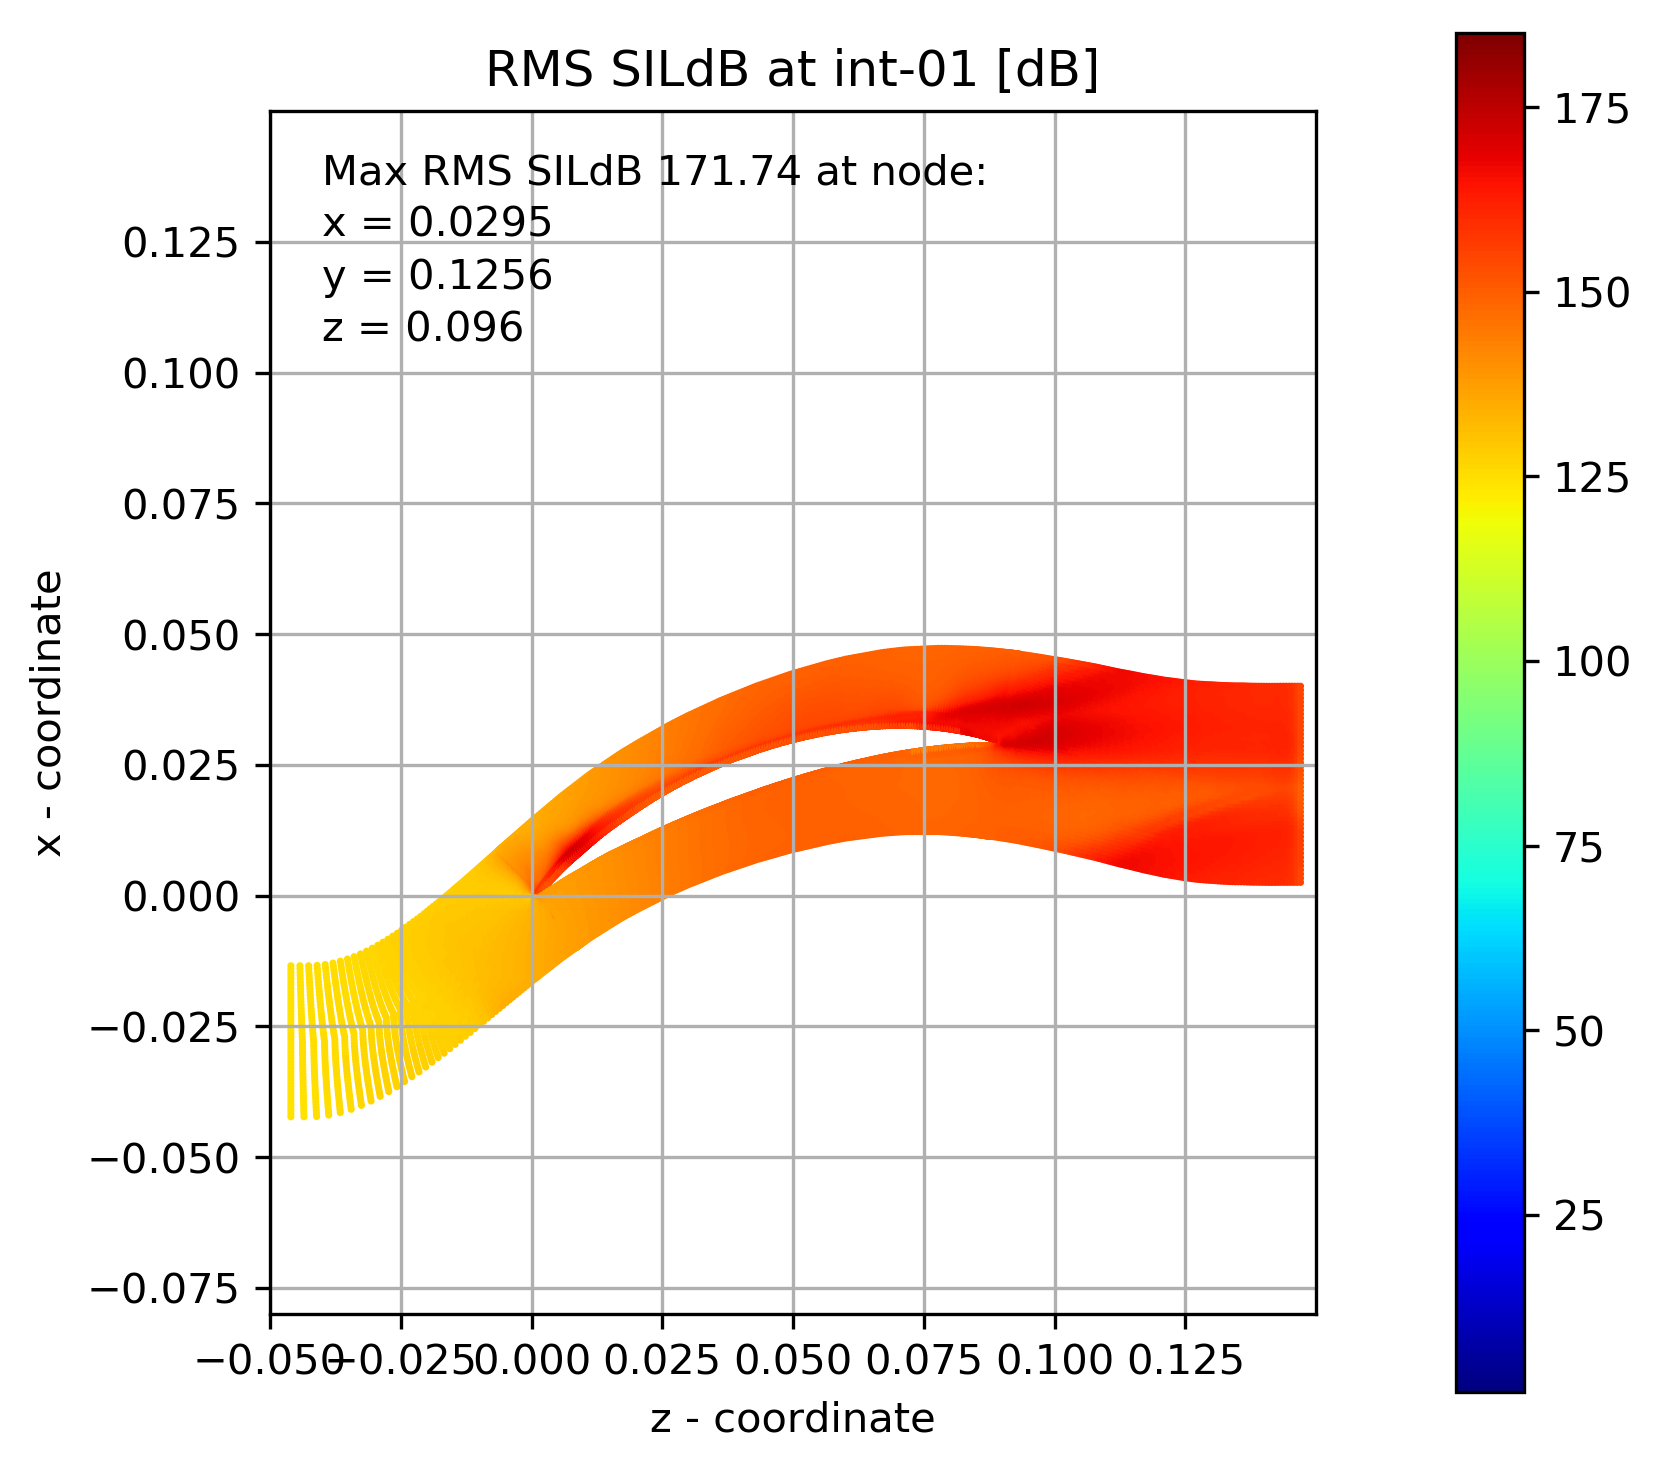
\includegraphics[width=0.75\textwidth]{Figures/int-01-rms-sildb.png}
  \caption{RMS Sound intensity decibel level at int-01 mark} \label{int-01-rms-sildb}
\end{figure}

%int-02
\begin{figure}[ht]
  \centering
  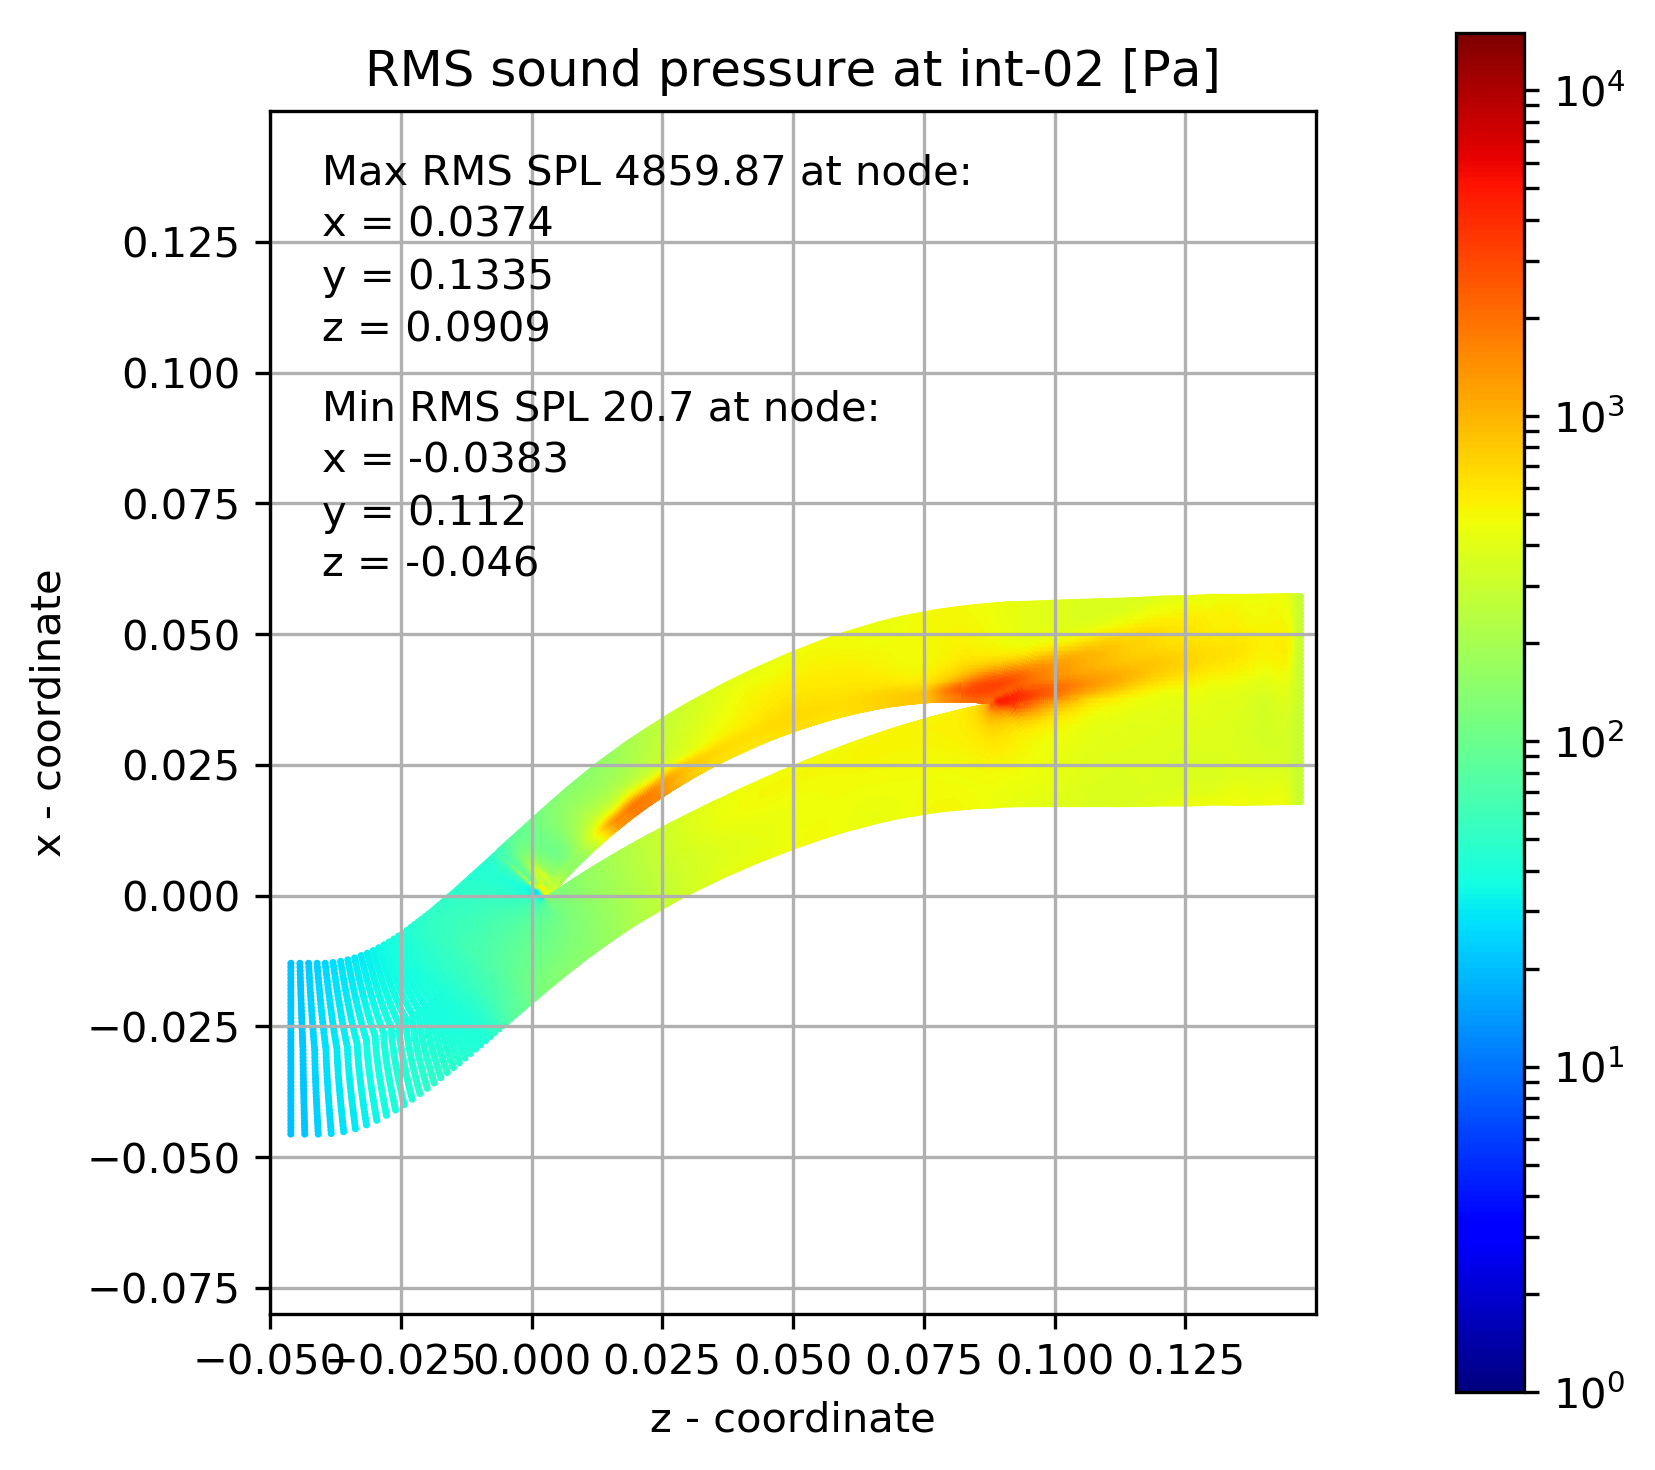
\includegraphics[width=0.75\textwidth]{Figures/int-02-rms-spl.png}
  \caption{RMS Sound pressure at int-02 mark} \label{int-02-rms-spl}
  
  \vspace*{\floatsep}% https://tex.stackexchange.com/q/26521/5764

  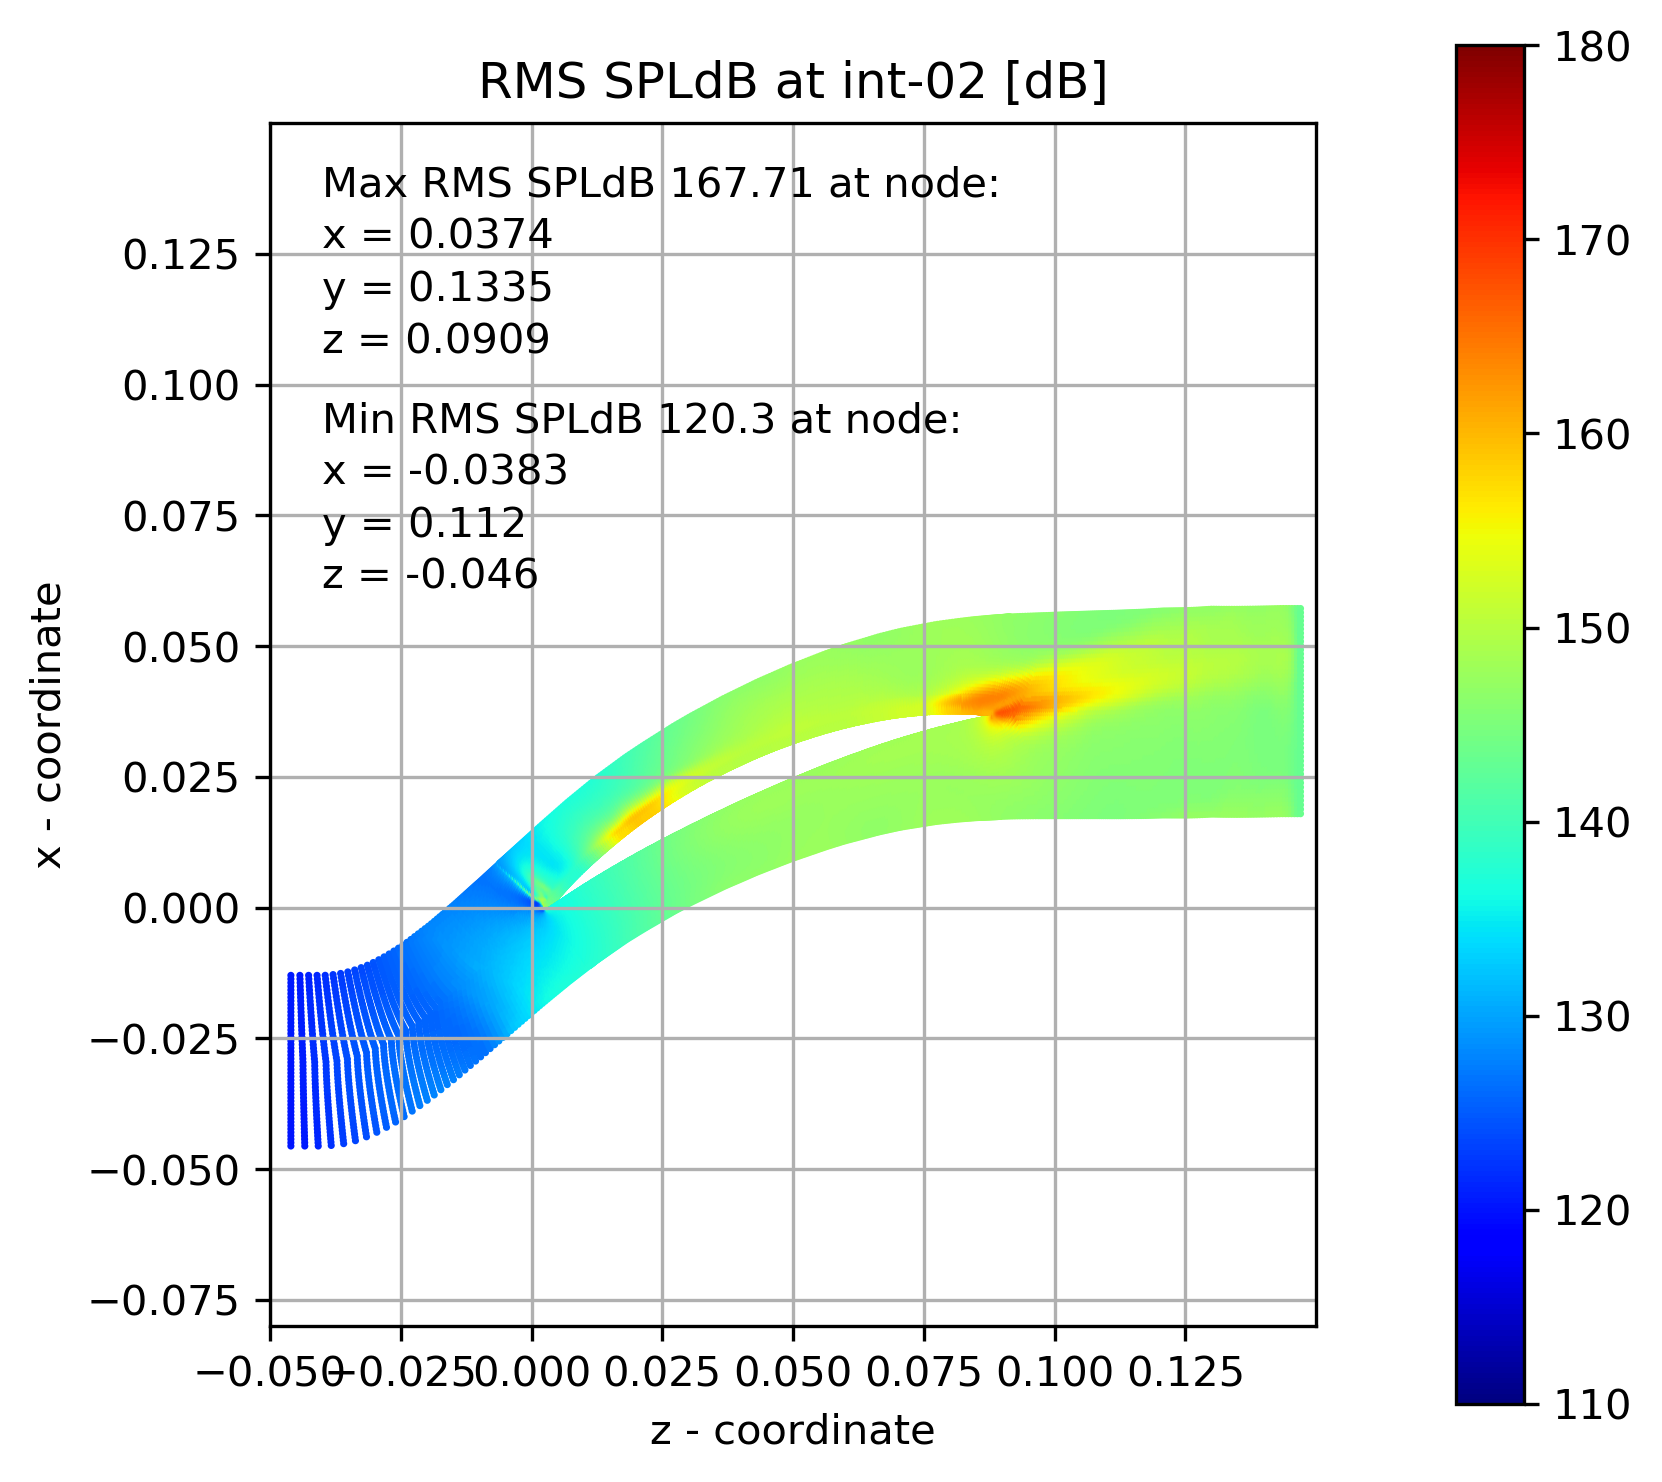
\includegraphics[width=0.75\textwidth]{Figures/int-02-rms-spldb.png}
  \caption{RMS Sound pressure decibel level at int-02 mark} \label{int-02-rms-spldb}
\end{figure}
%int-02
\begin{figure}[ht]
  \centering
  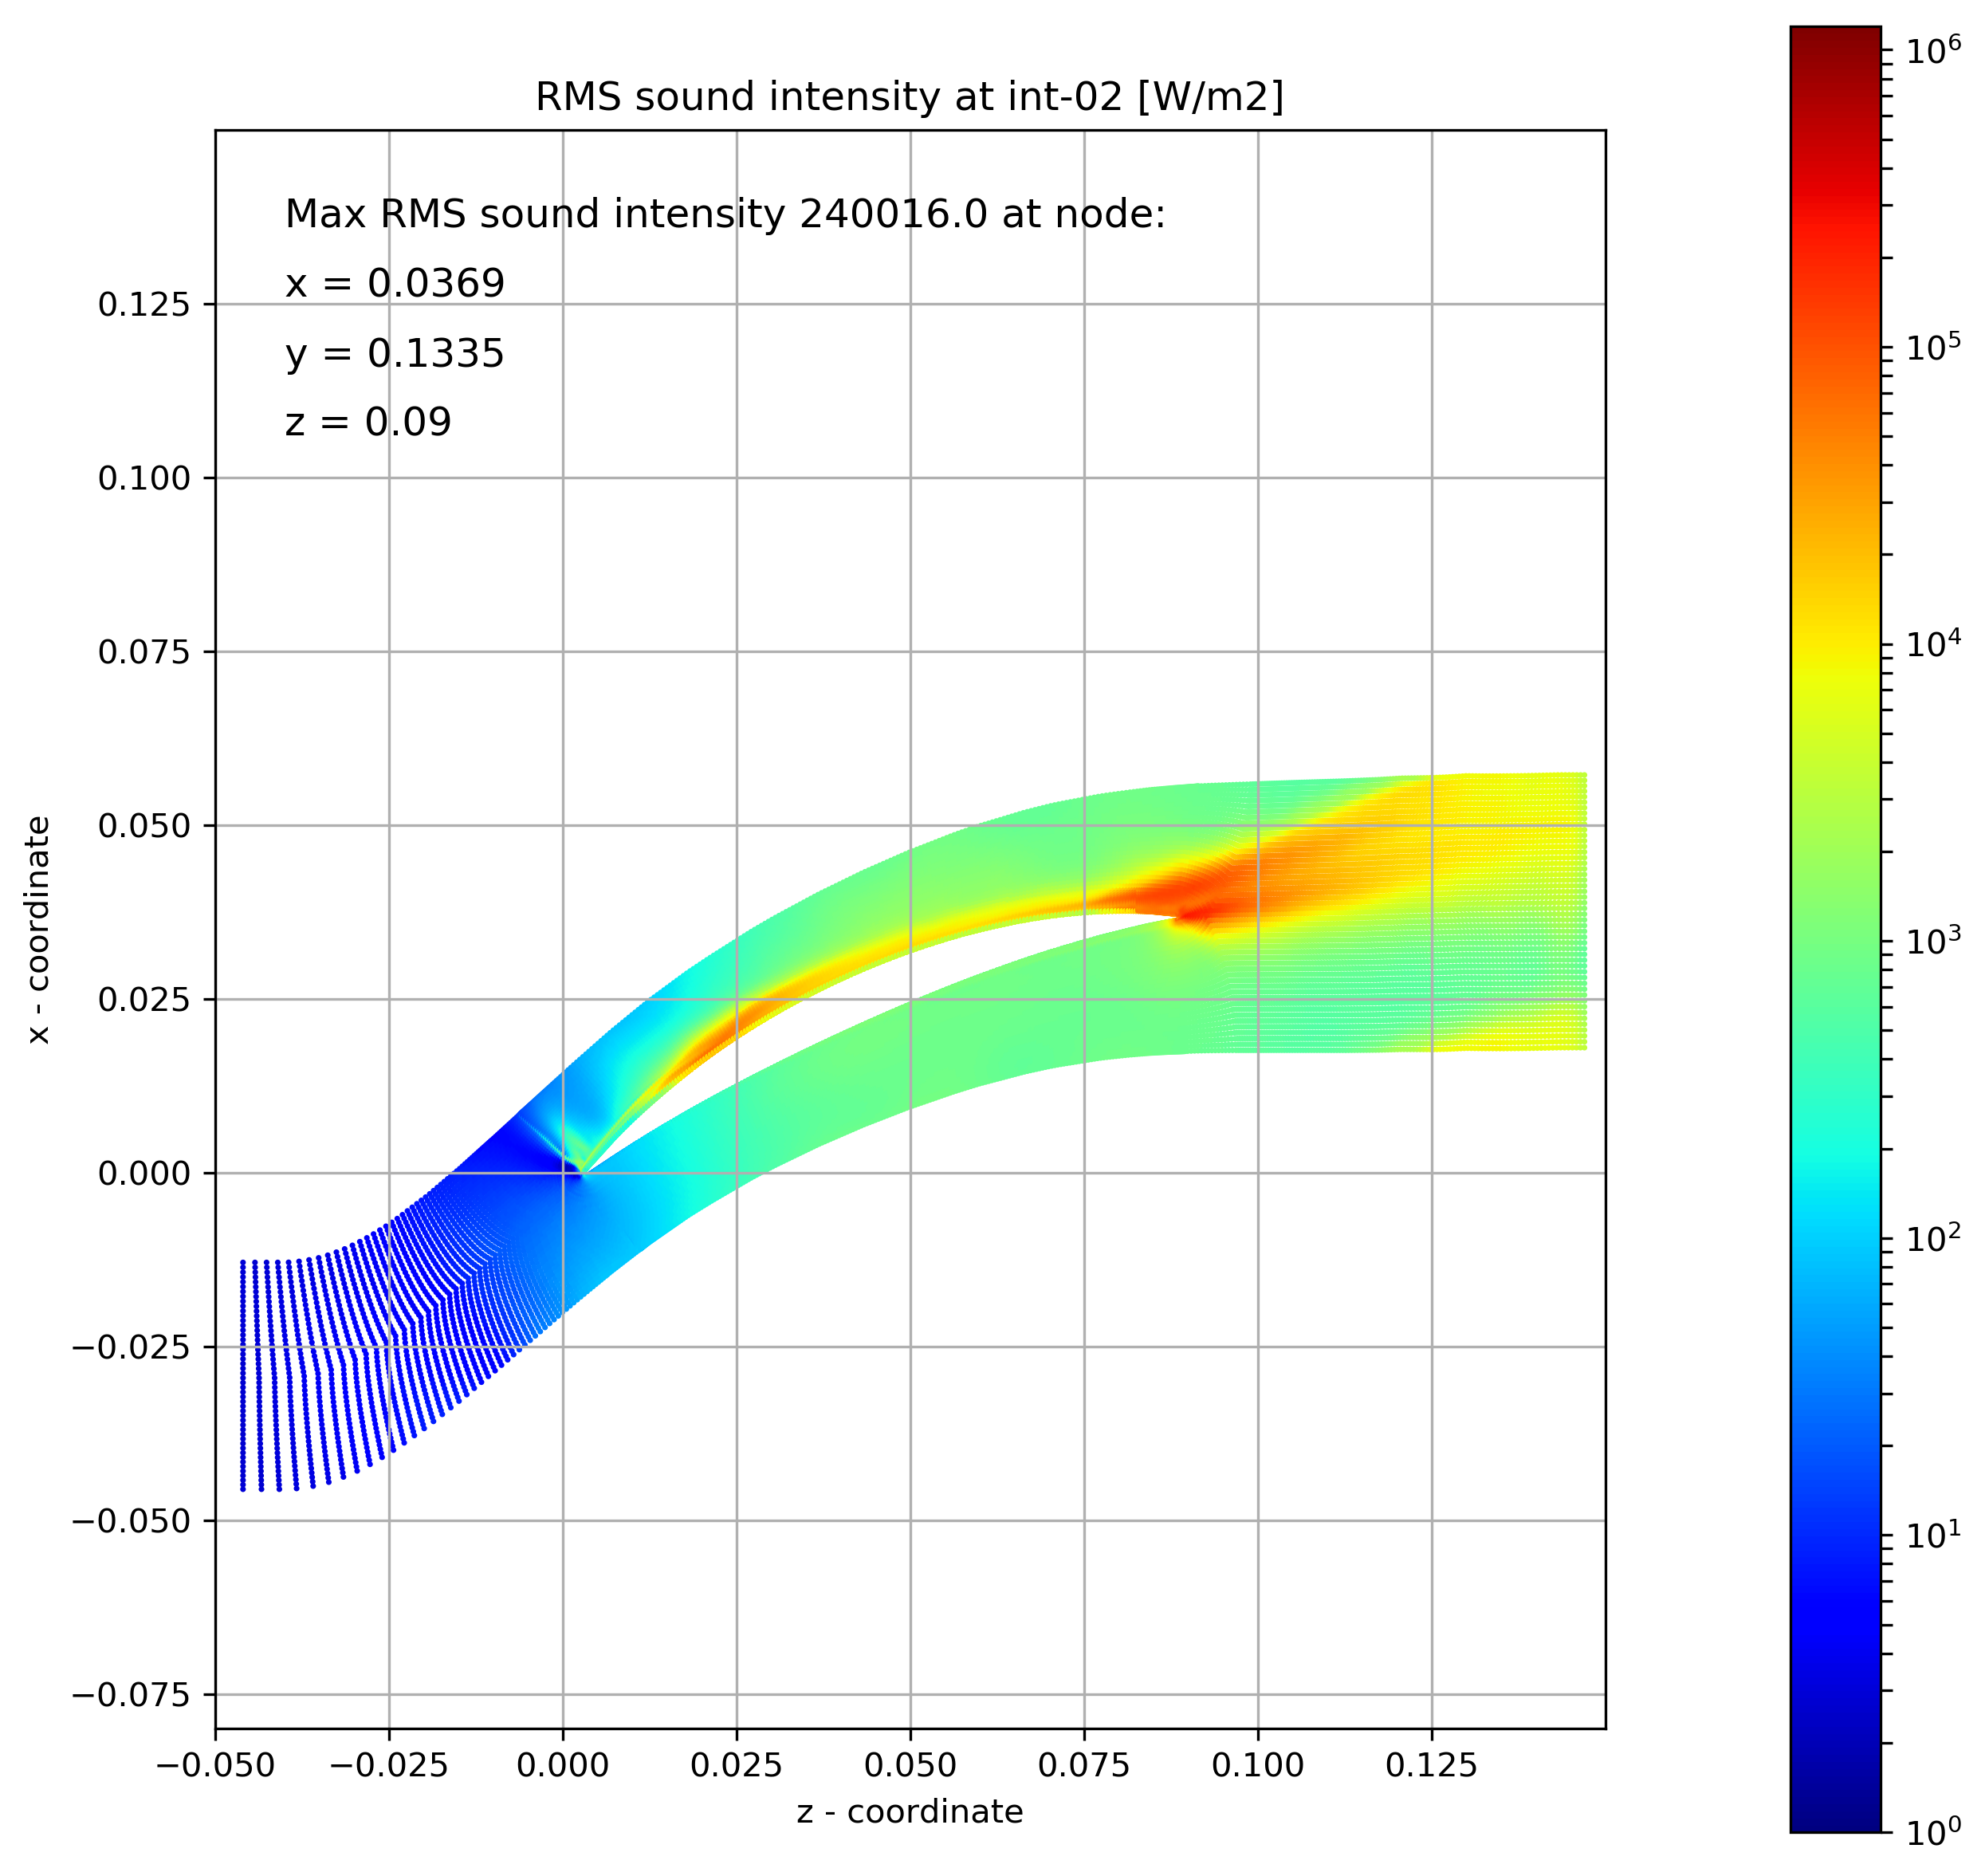
\includegraphics[width=0.75\textwidth]{Figures/int-02-rms-sil.png}
  \caption{RMS Sound intensity at int-02 mark} \label{int-02-rms-sil}
  
  \vspace*{\floatsep}% https://tex.stackexchange.com/q/26521/5764

  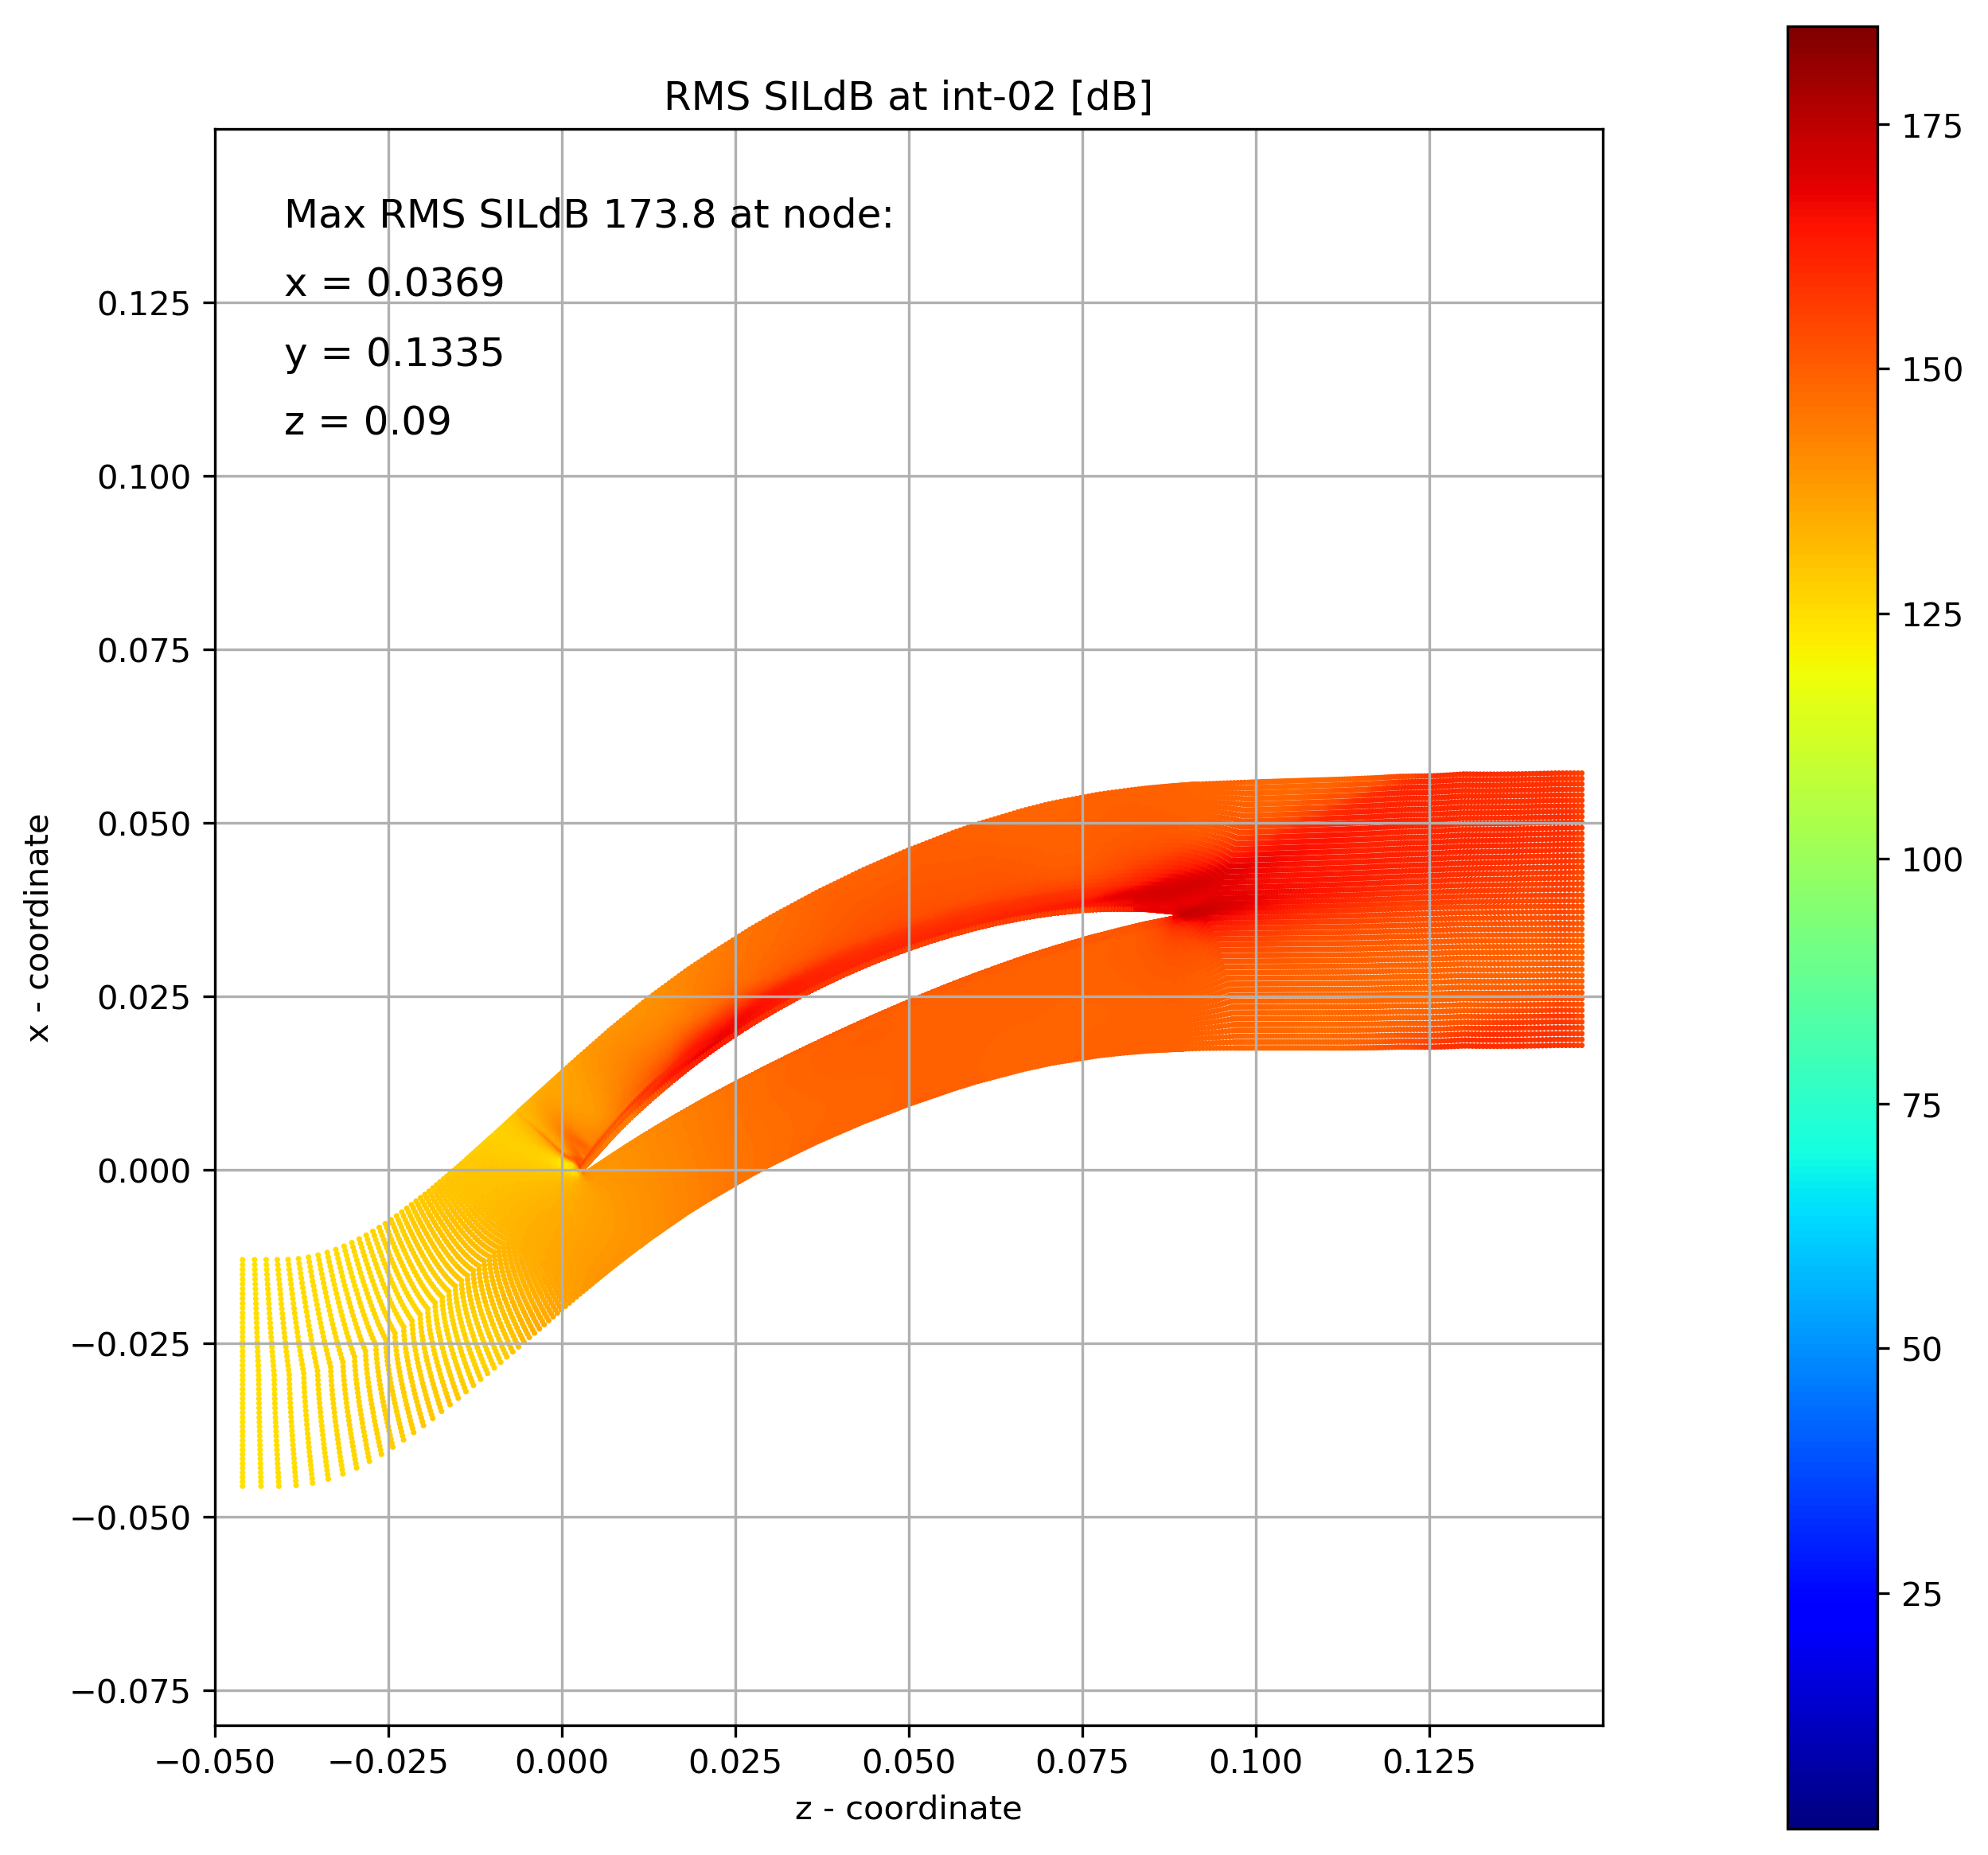
\includegraphics[width=0.75\textwidth]{Figures/int-02-rms-sildb.png}
  \caption{RMS Sound intensity decibel level at int-02 mark} \label{int-02-rms-sildb}
\end{figure}

%int-03
\begin{figure}[ht]
  \centering
  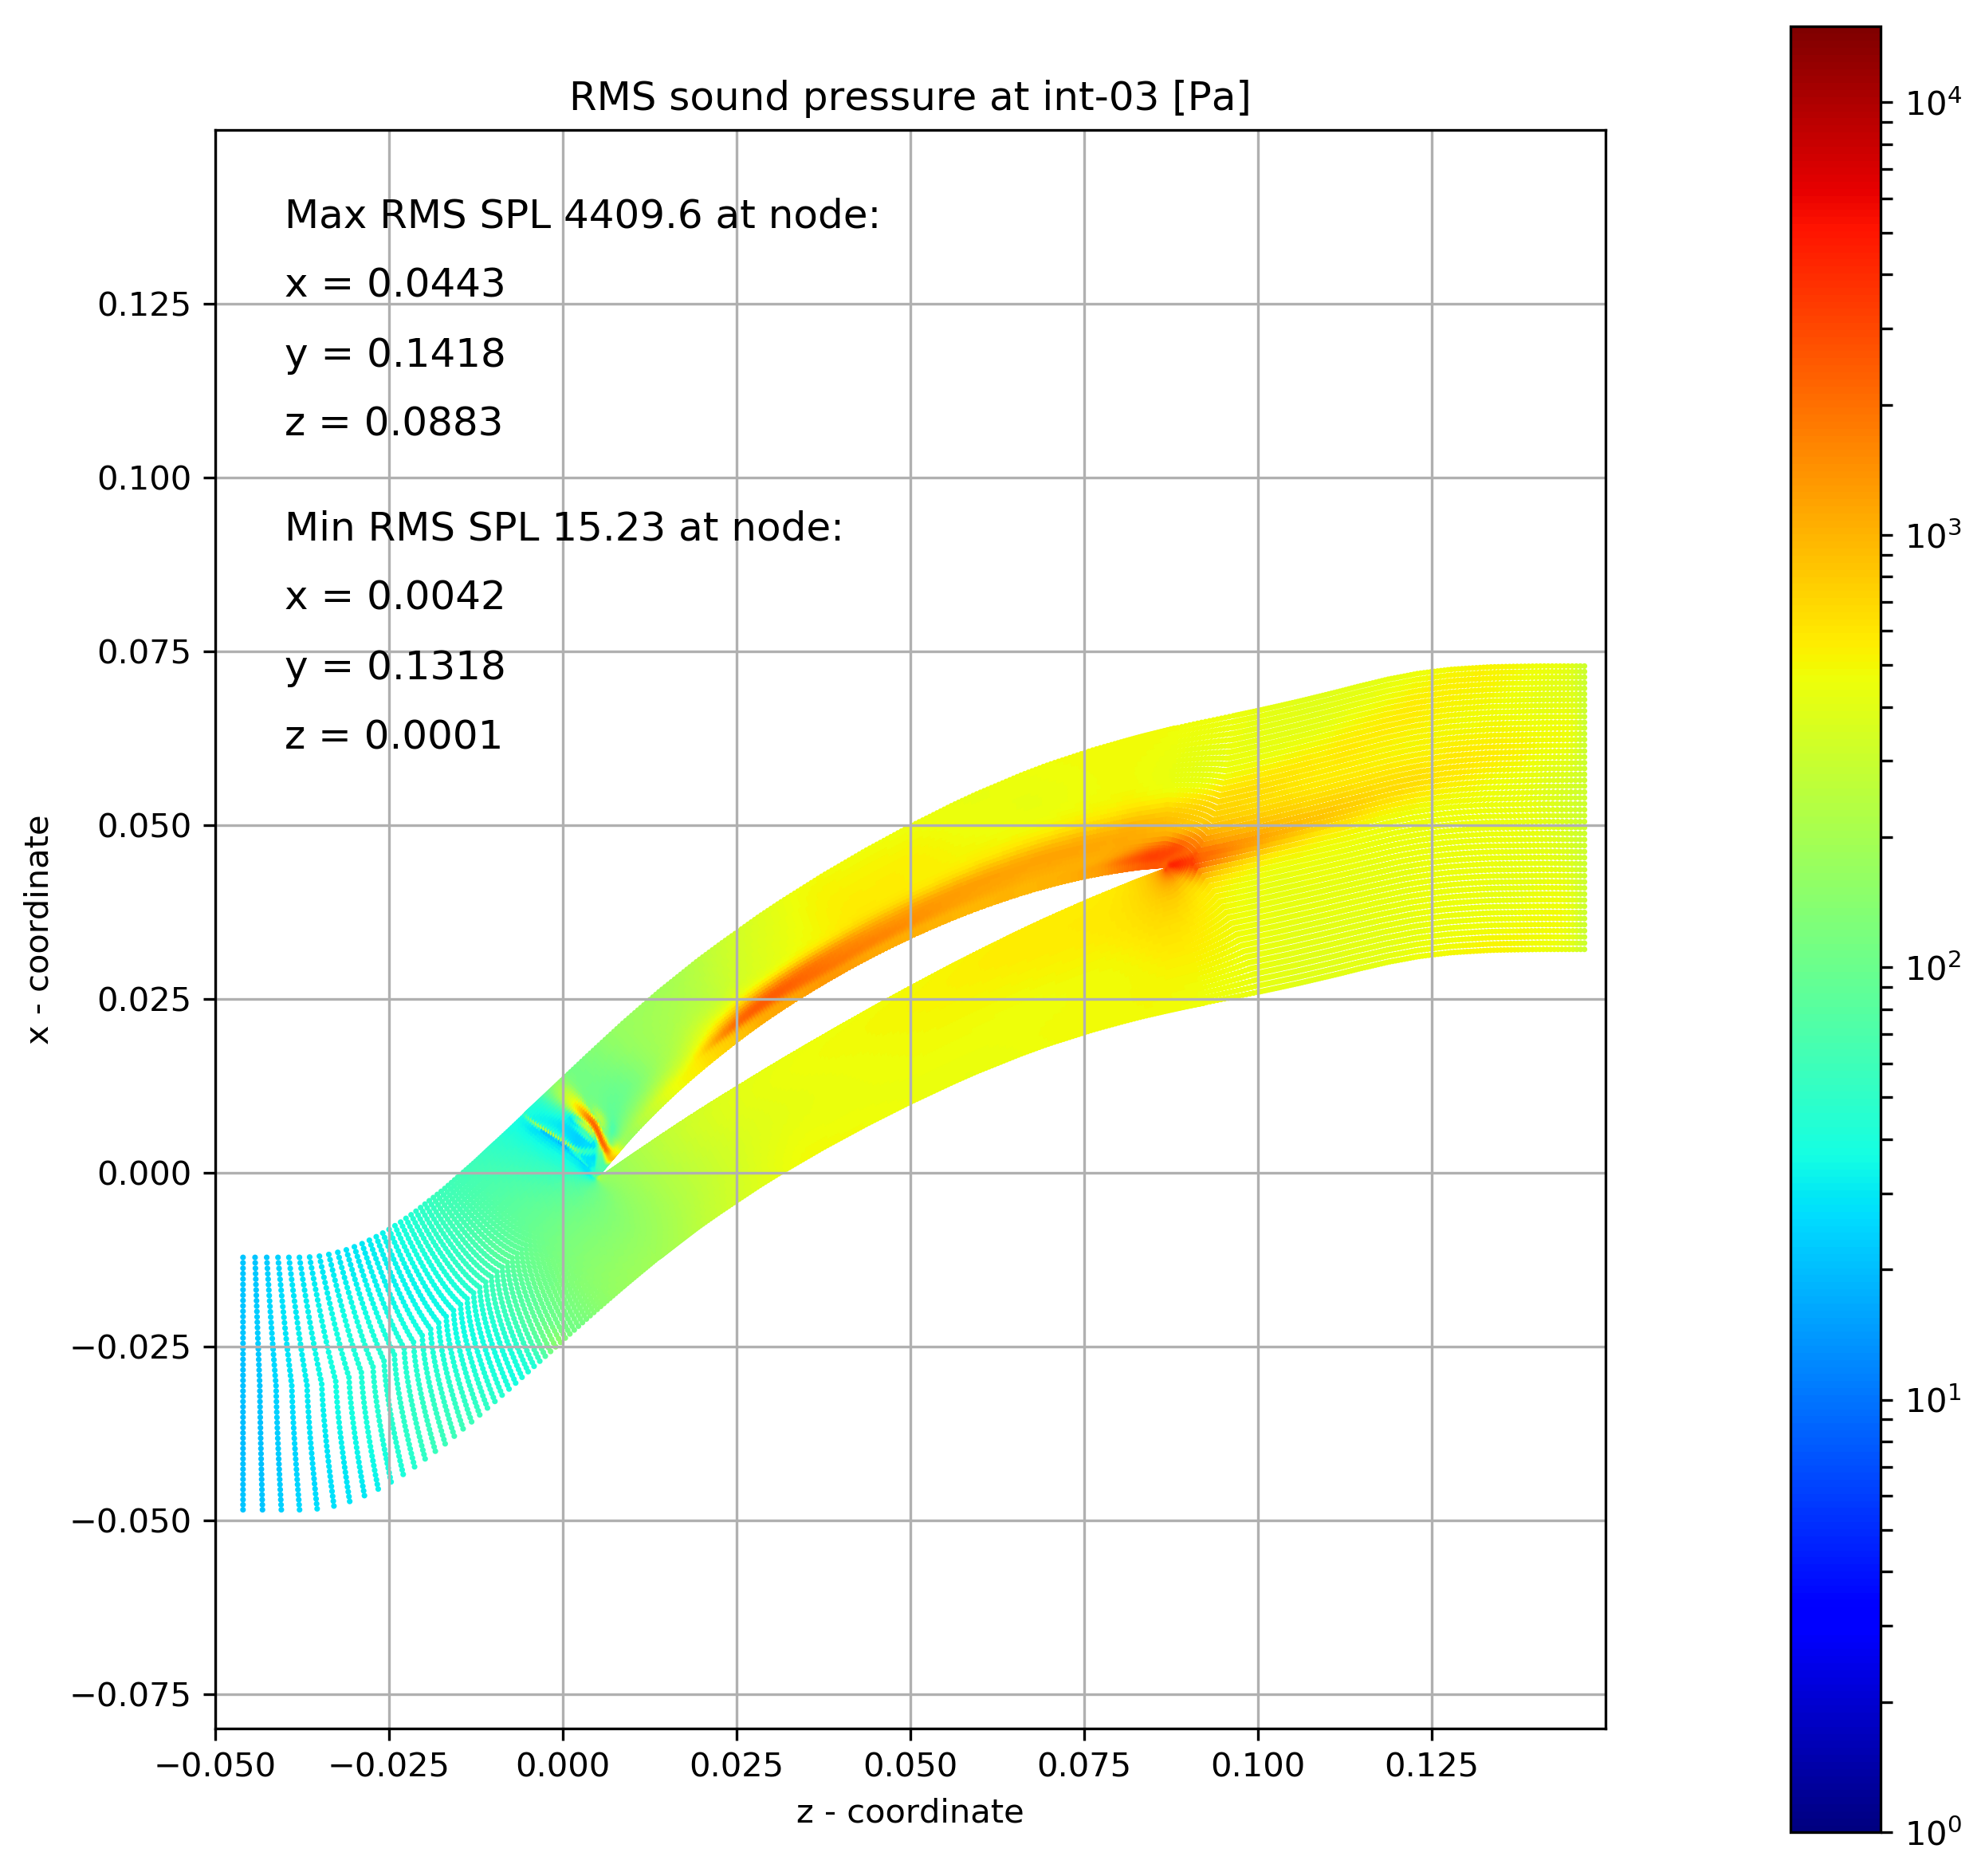
\includegraphics[width=0.75\textwidth]{Figures/int-03-rms-spl.png}
  \caption{RMS Sound pressure at int-03 mark} \label{int-03-rms-spl}
  
  \vspace*{\floatsep}% https://tex.stackexchange.com/q/26521/5764

  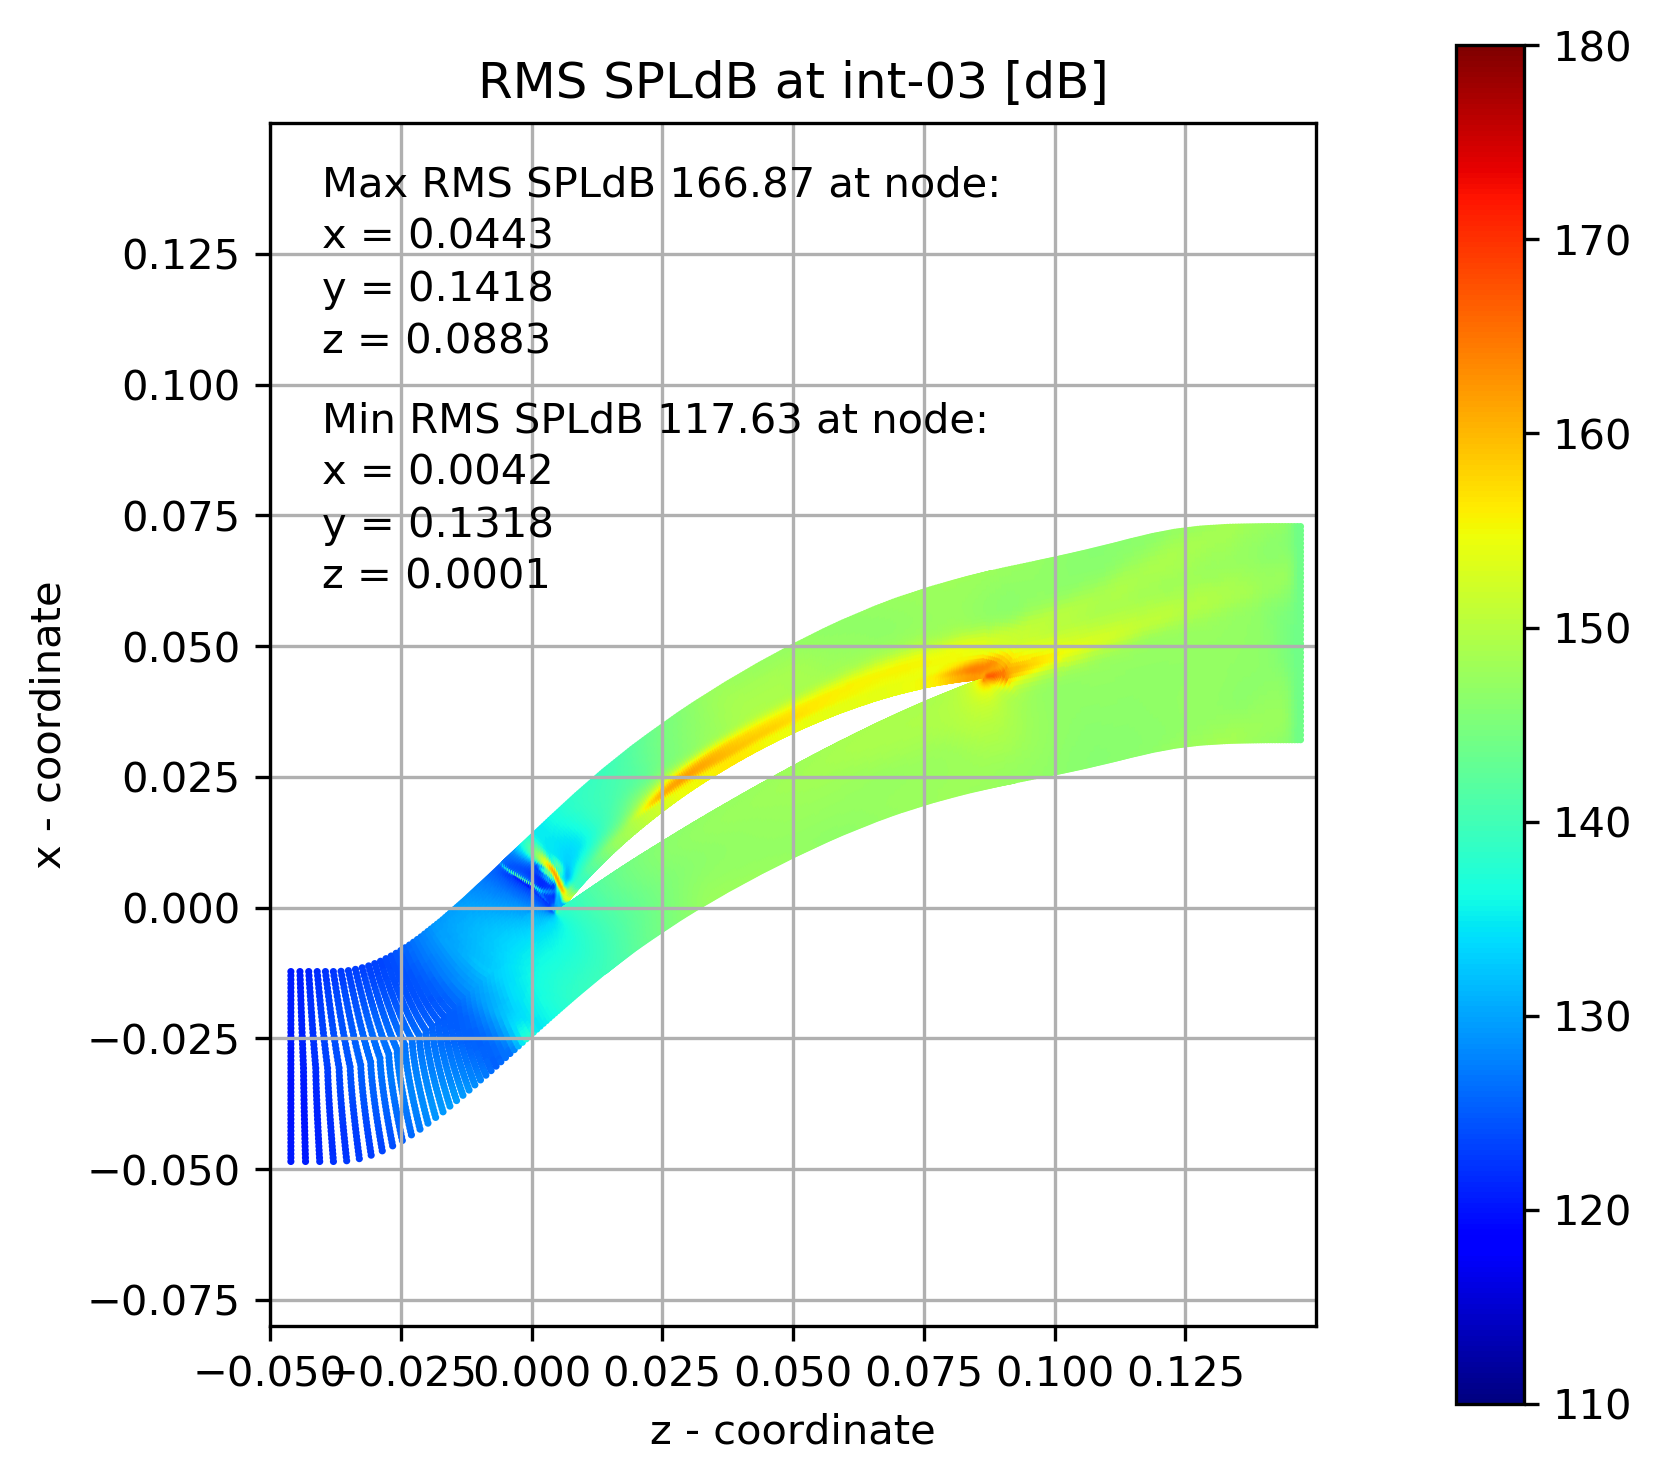
\includegraphics[width=0.75\textwidth]{Figures/int-03-rms-spldb.png}
  \caption{RMS Sound pressure decibel level at int-03 mark} \label{int-03-rms-spldb}
\end{figure}
%int-03
\begin{figure}[ht]
  \centering
  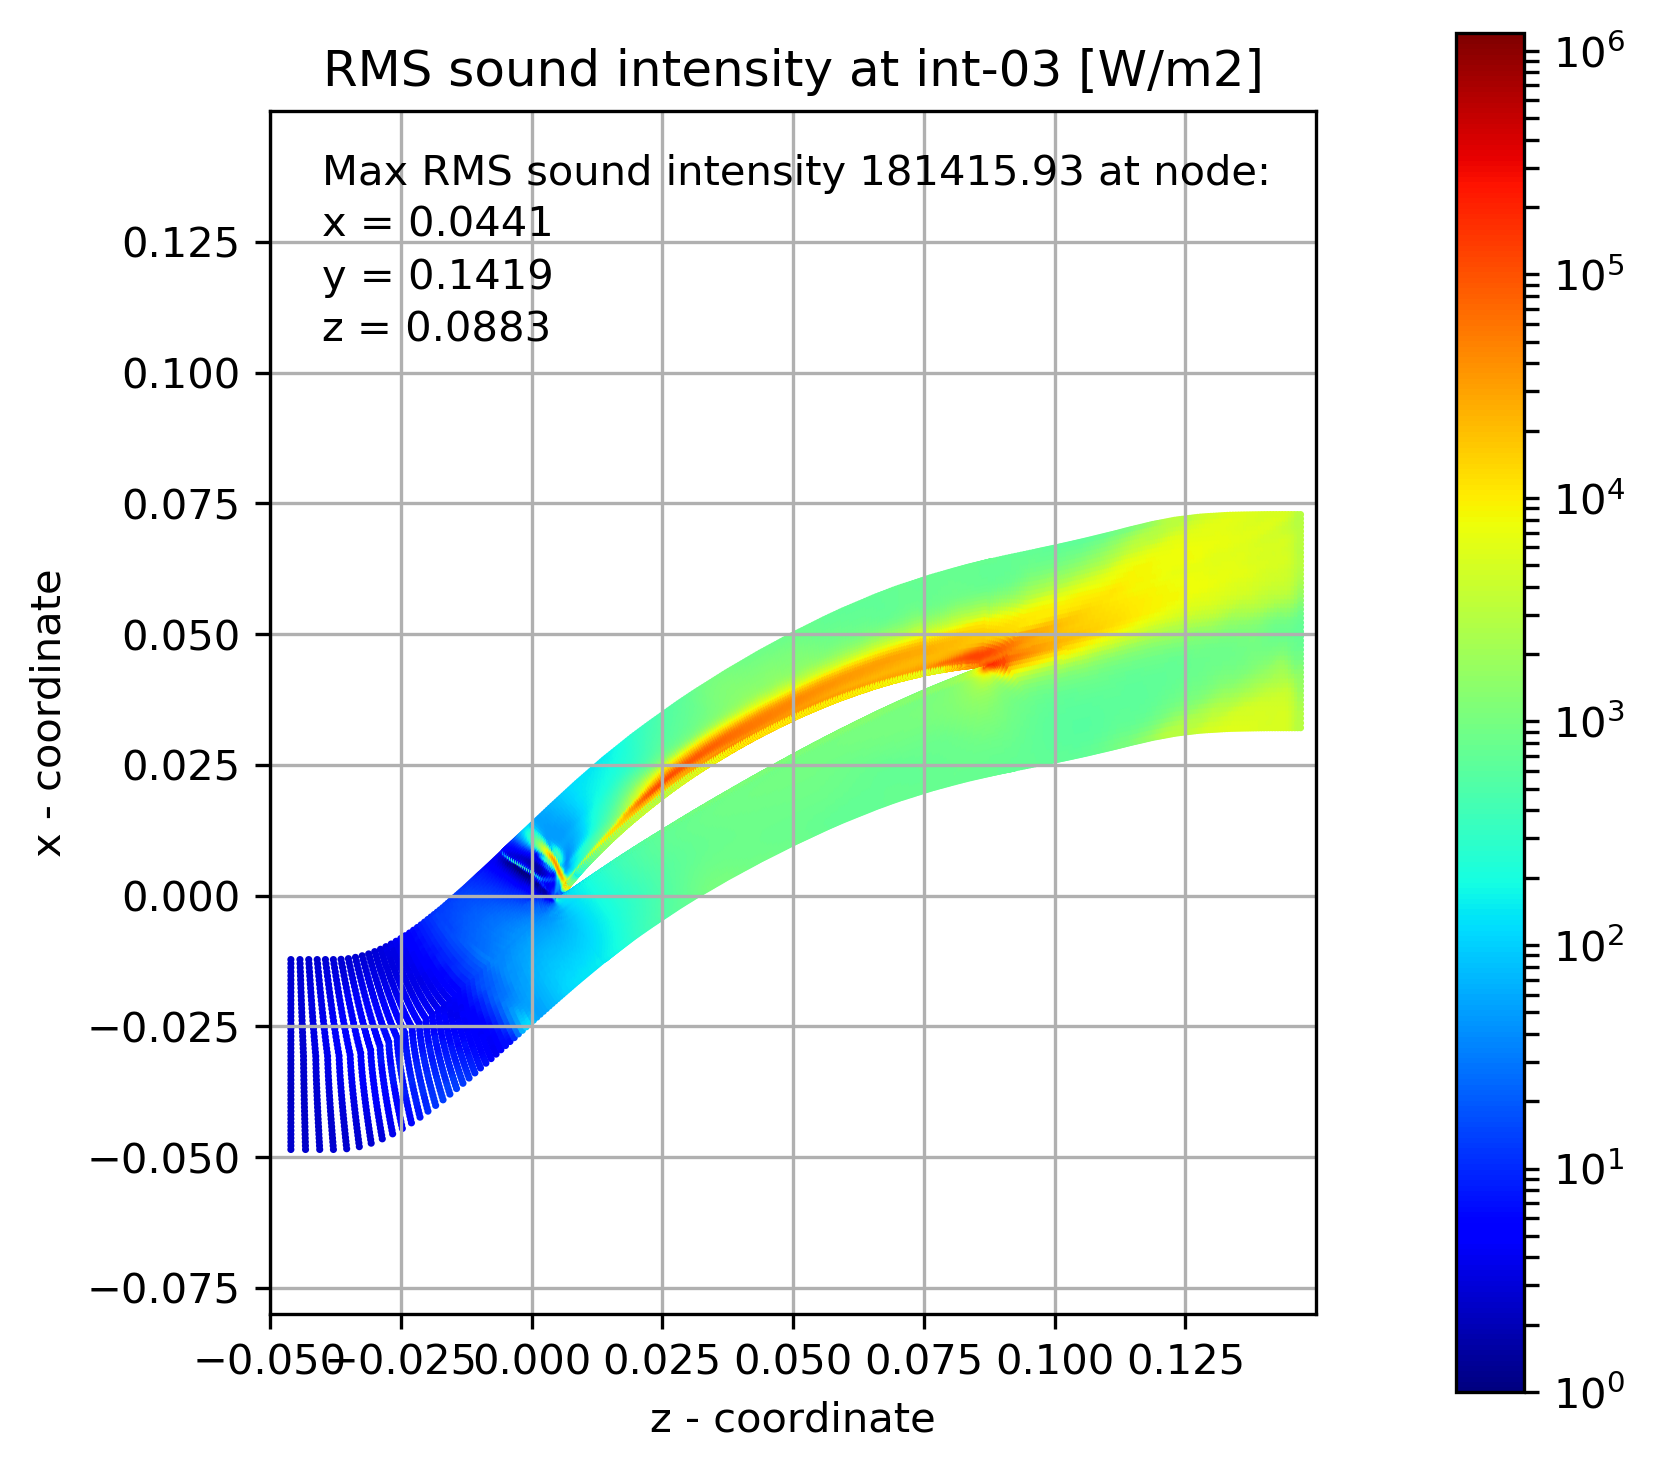
\includegraphics[width=0.75\textwidth]{Figures/int-03-rms-sil.png}
  \caption{RMS Sound intensity at int-03 mark} \label{int-03-rms-sil}
  
  \vspace*{\floatsep}% https://tex.stackexchange.com/q/26521/5764

  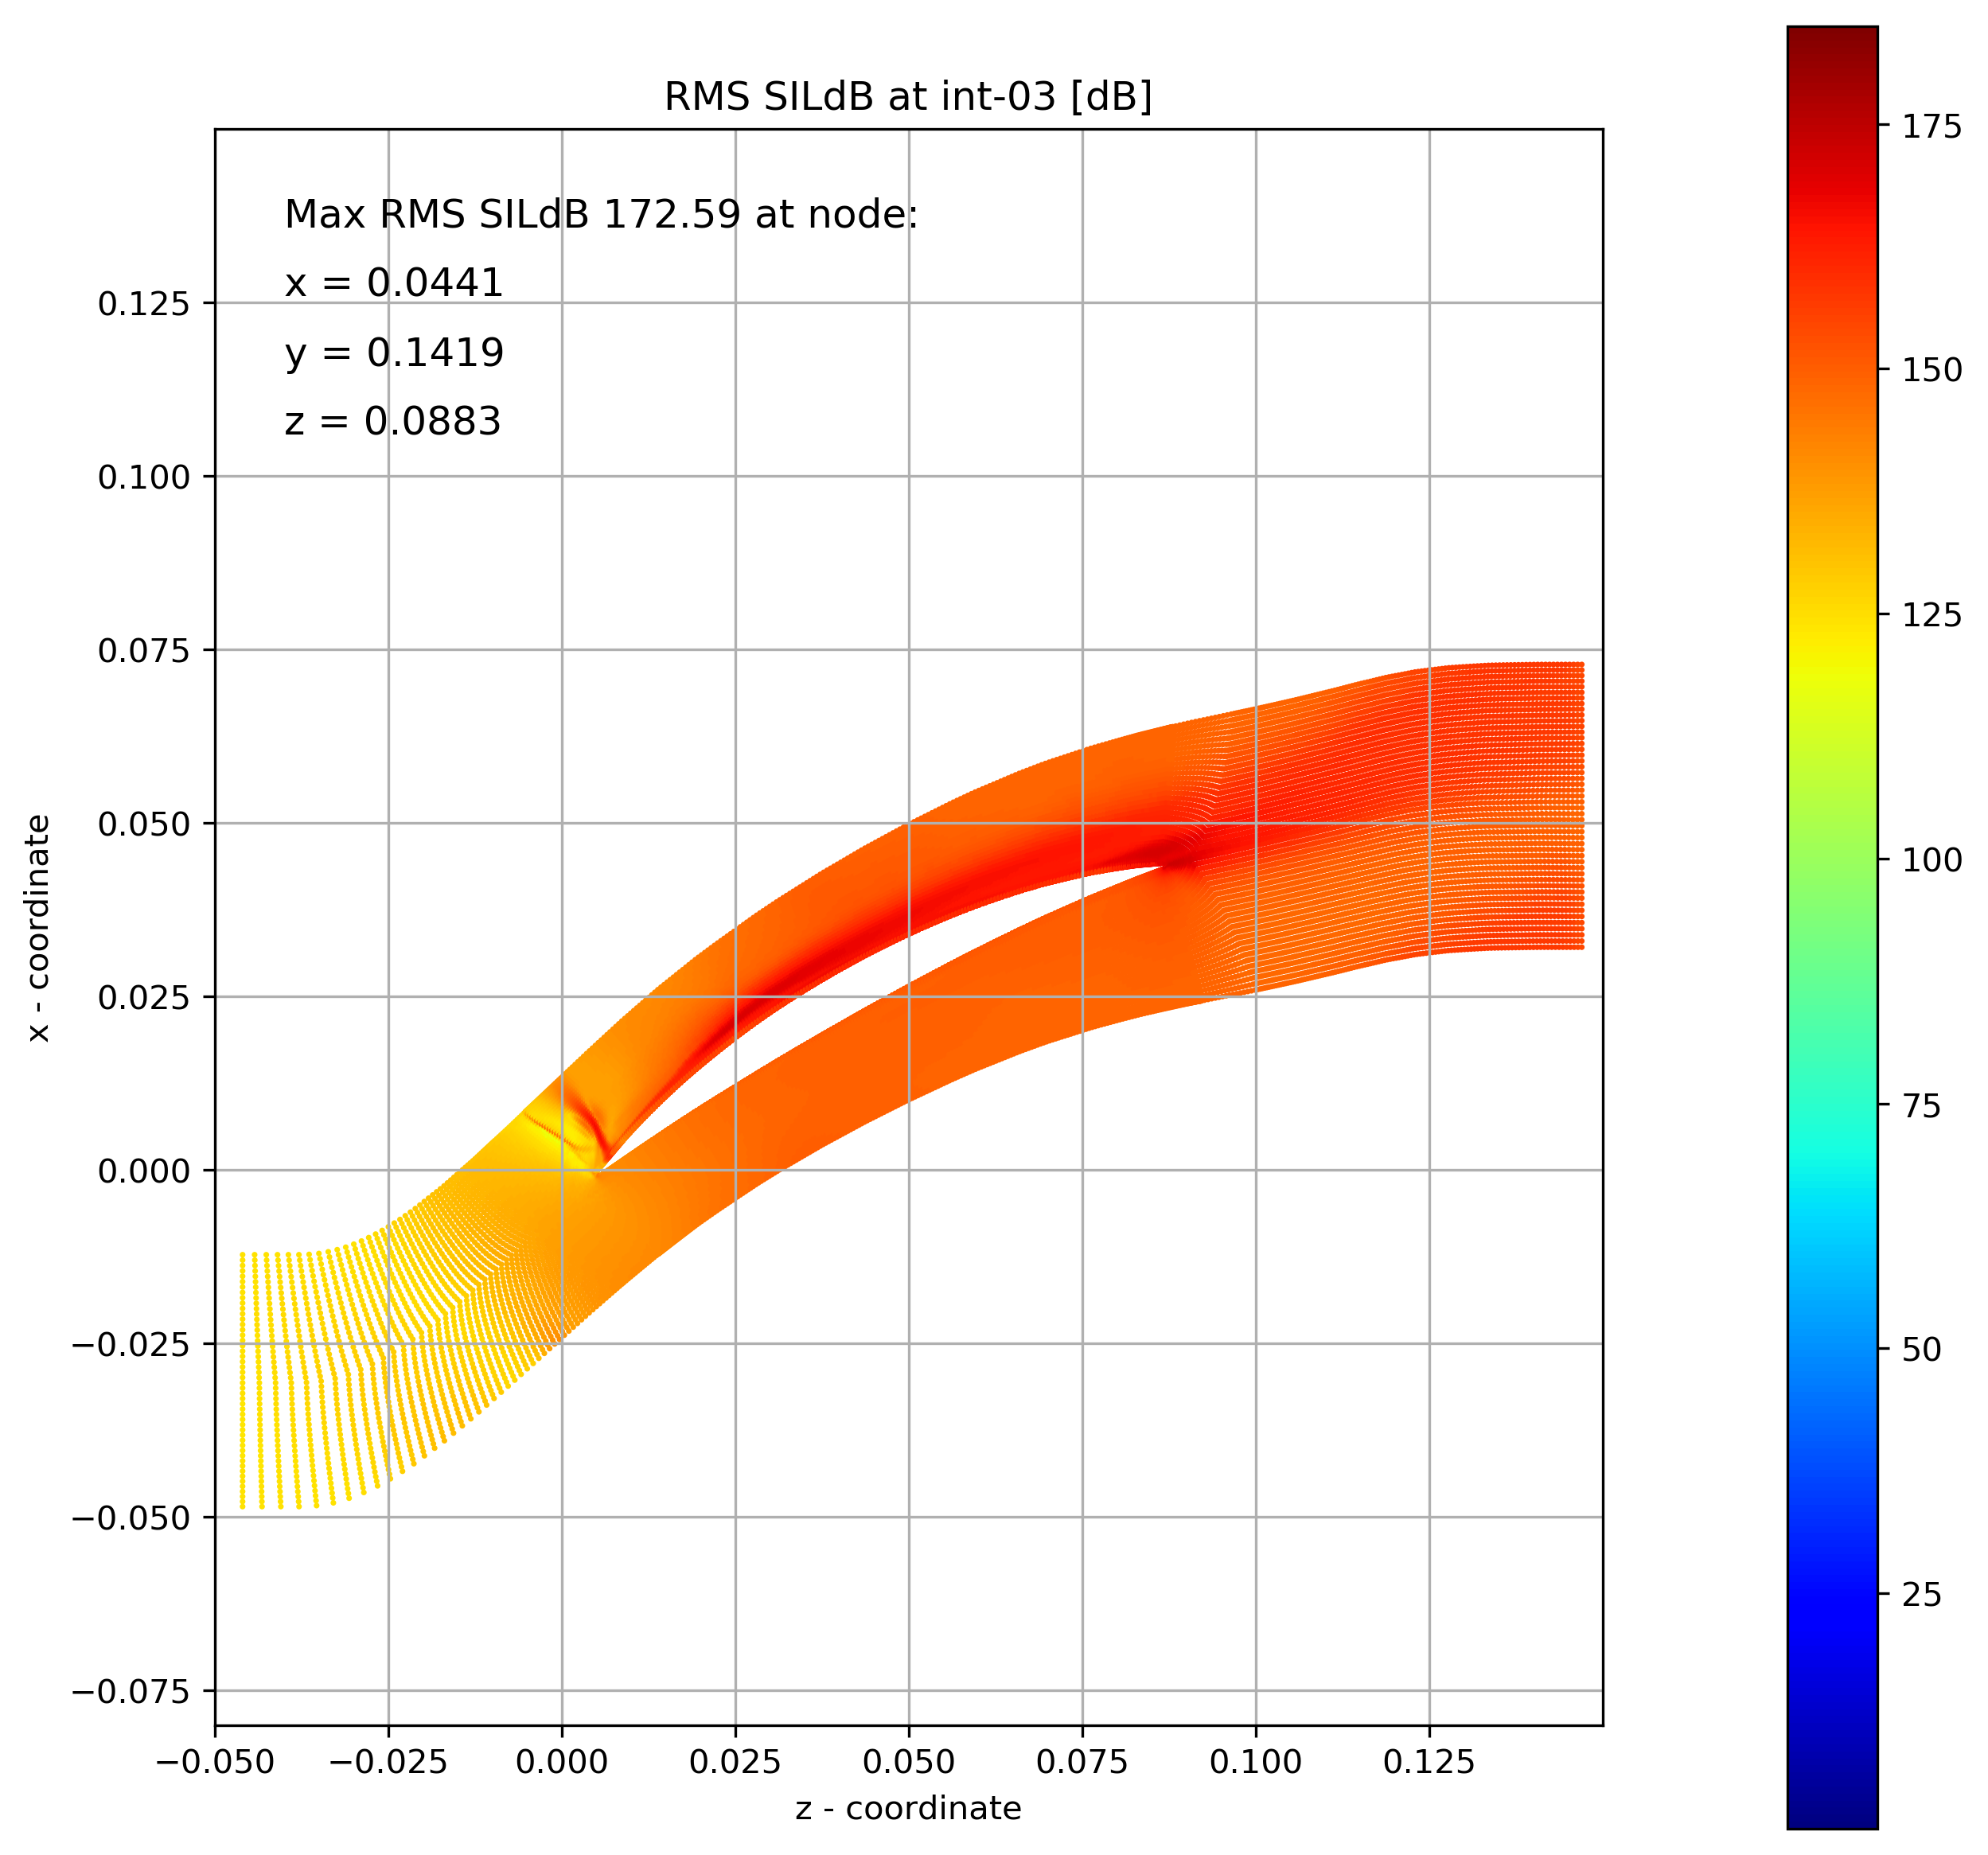
\includegraphics[width=0.75\textwidth]{Figures/int-03-rms-sildb.png}
  \caption{RMS Sound intensity decibel level at int-03 mark} \label{int-03-rms-sildb}
\end{figure}

%int-04
\begin{figure}[ht]
  \centering
  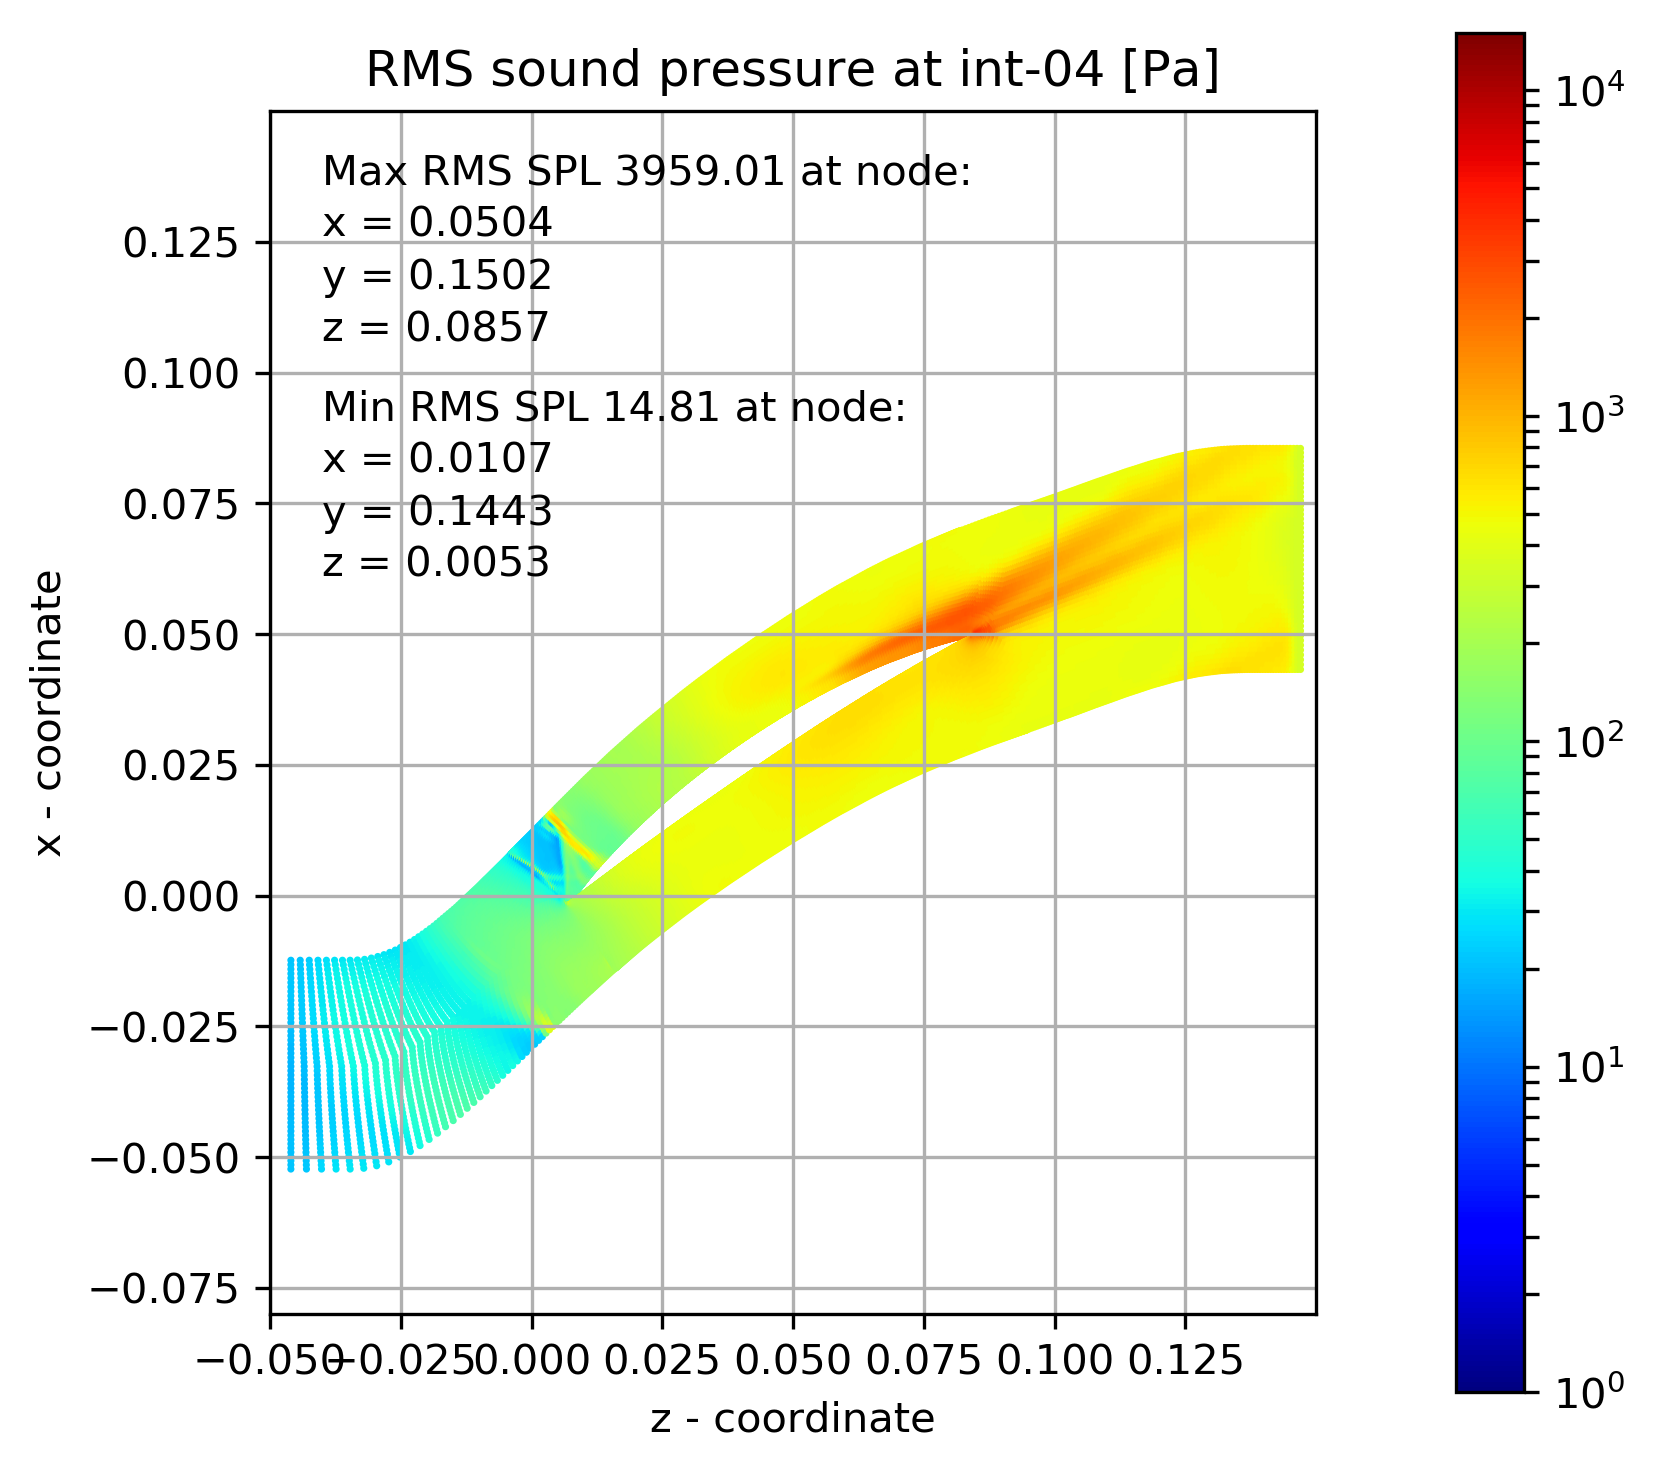
\includegraphics[width=0.75\textwidth]{Figures/int-04-rms-spl.png}
  \caption{RMS Sound pressure at int-04 mark} \label{int-04-rms-spl}
  
  \vspace*{\floatsep}% https://tex.stackexchange.com/q/26521/5764

  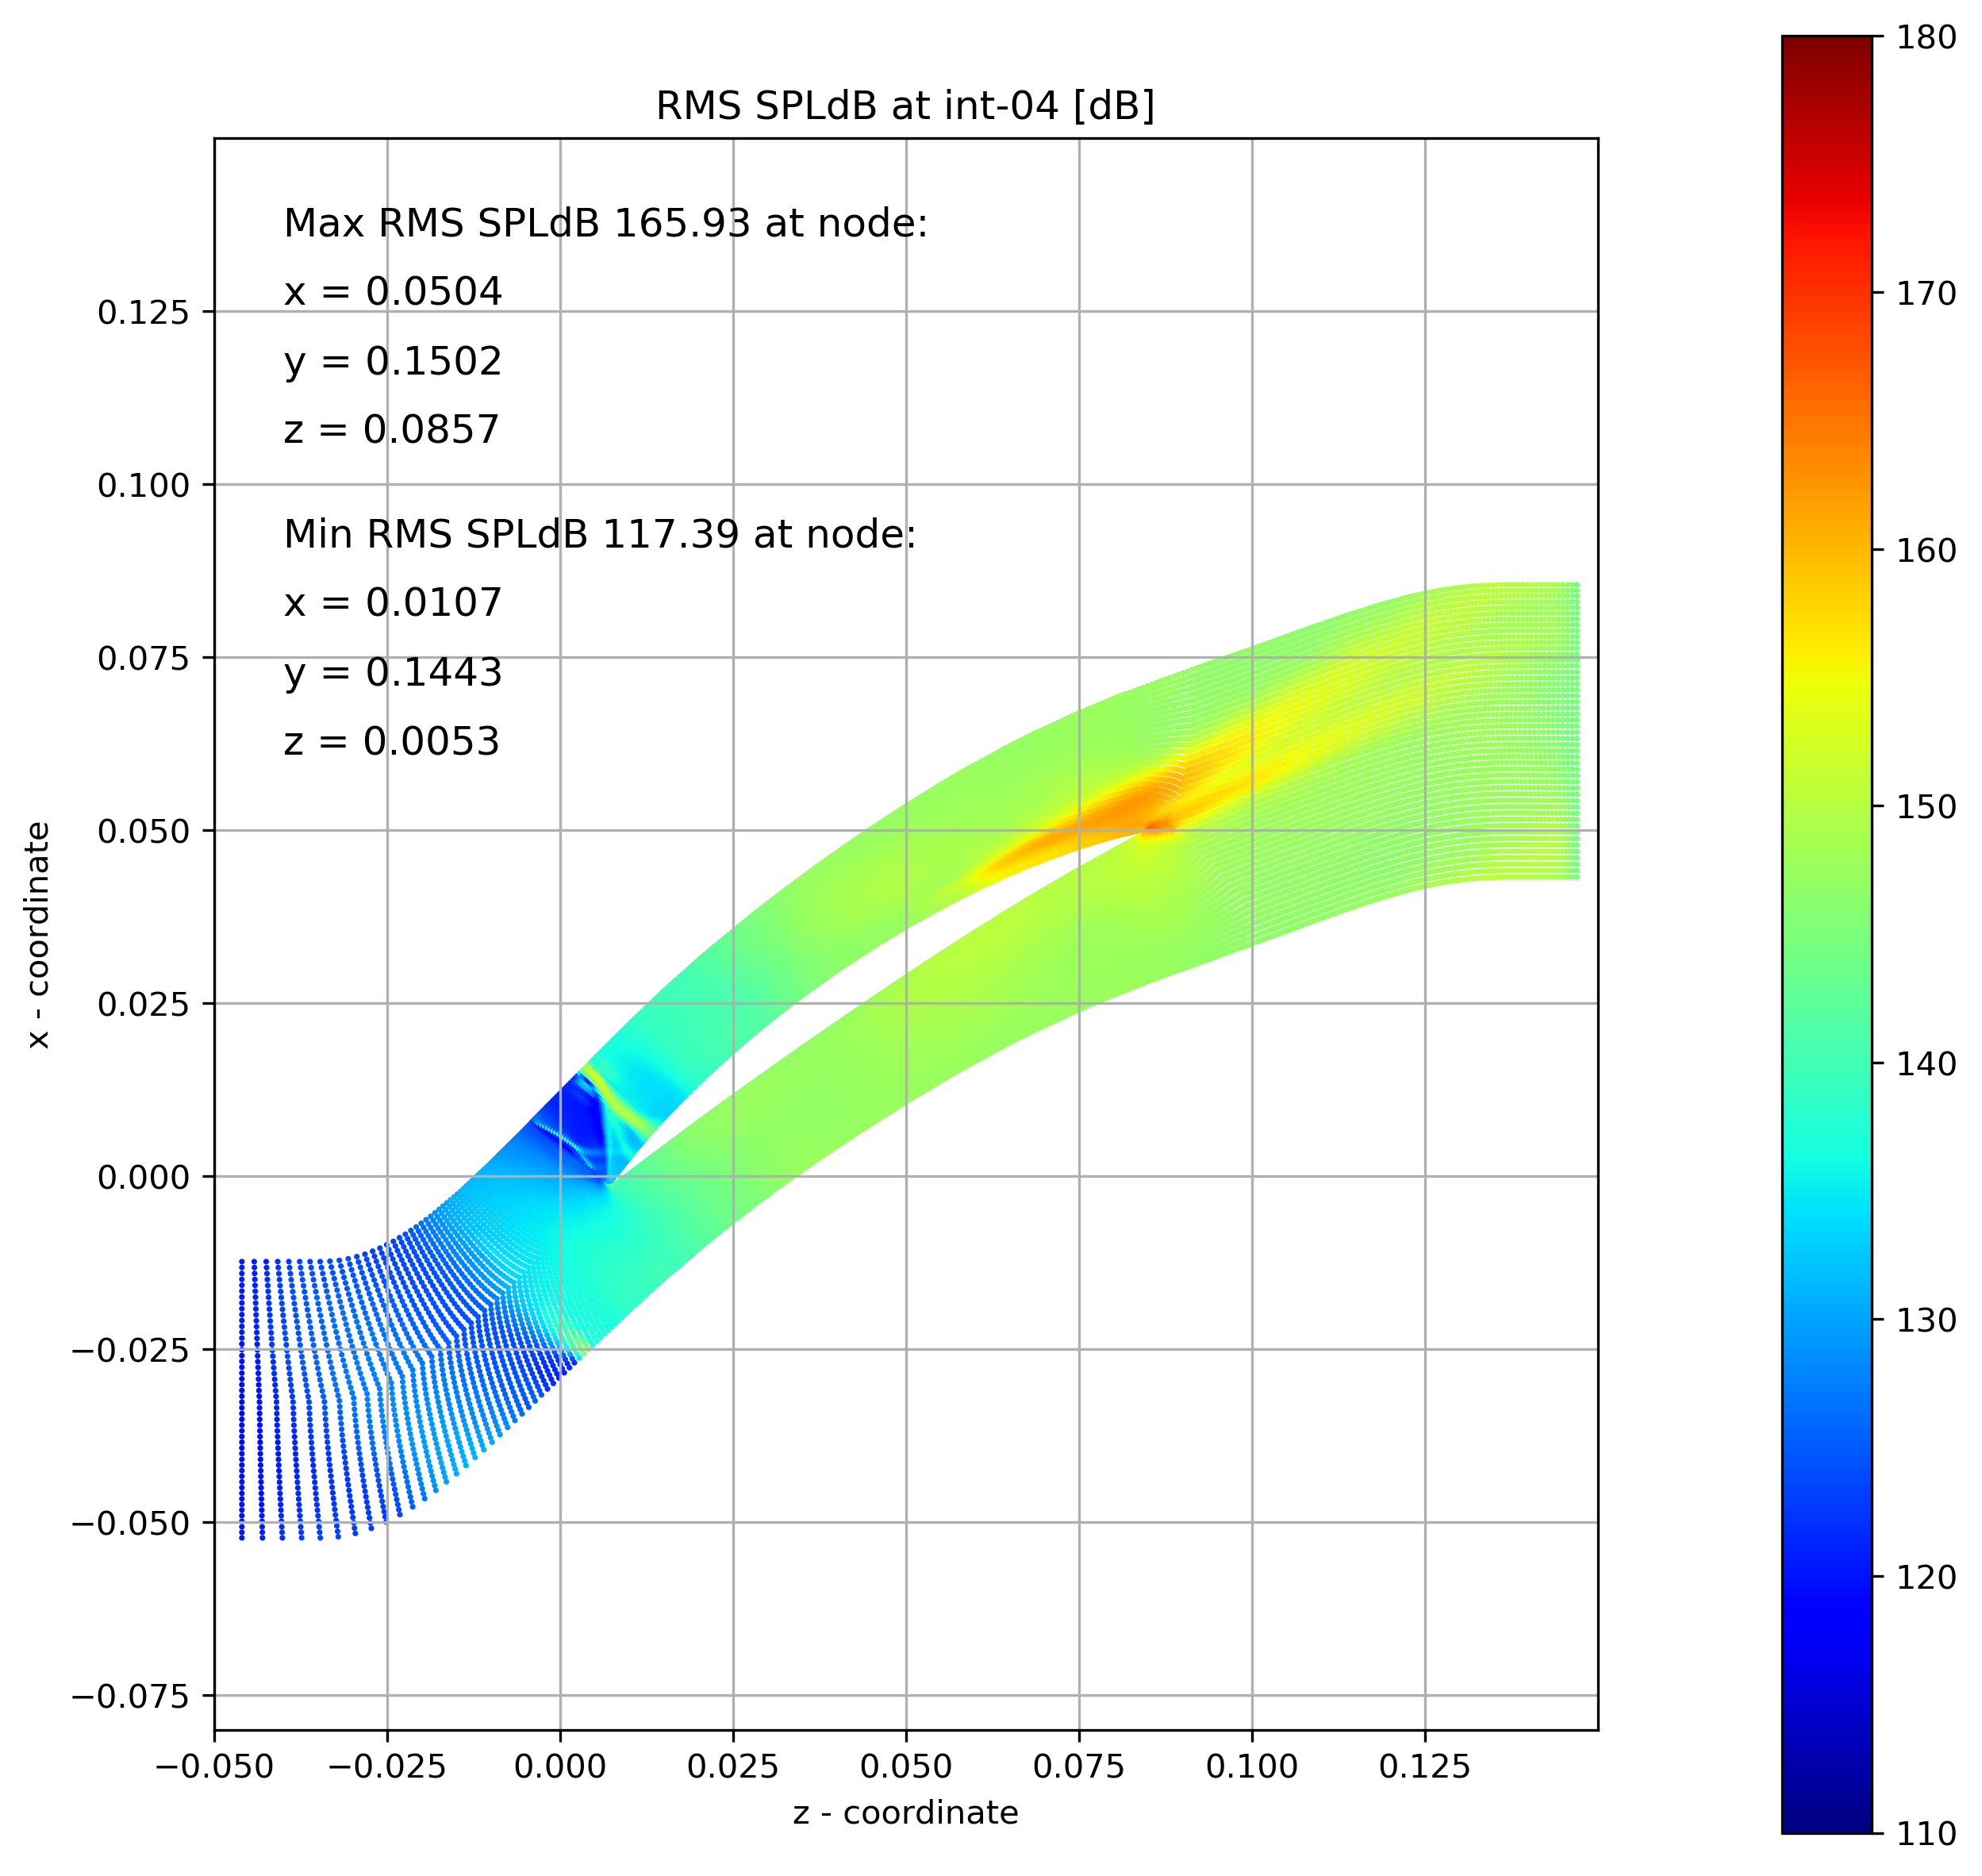
\includegraphics[width=0.75\textwidth]{Figures/int-04-rms-spldb.png}
  \caption{RMS Sound pressure decibel level at int-04 mark} \label{int-04-rms-spldb}
\end{figure}
%int-04
\begin{figure}[ht]
  \centering
  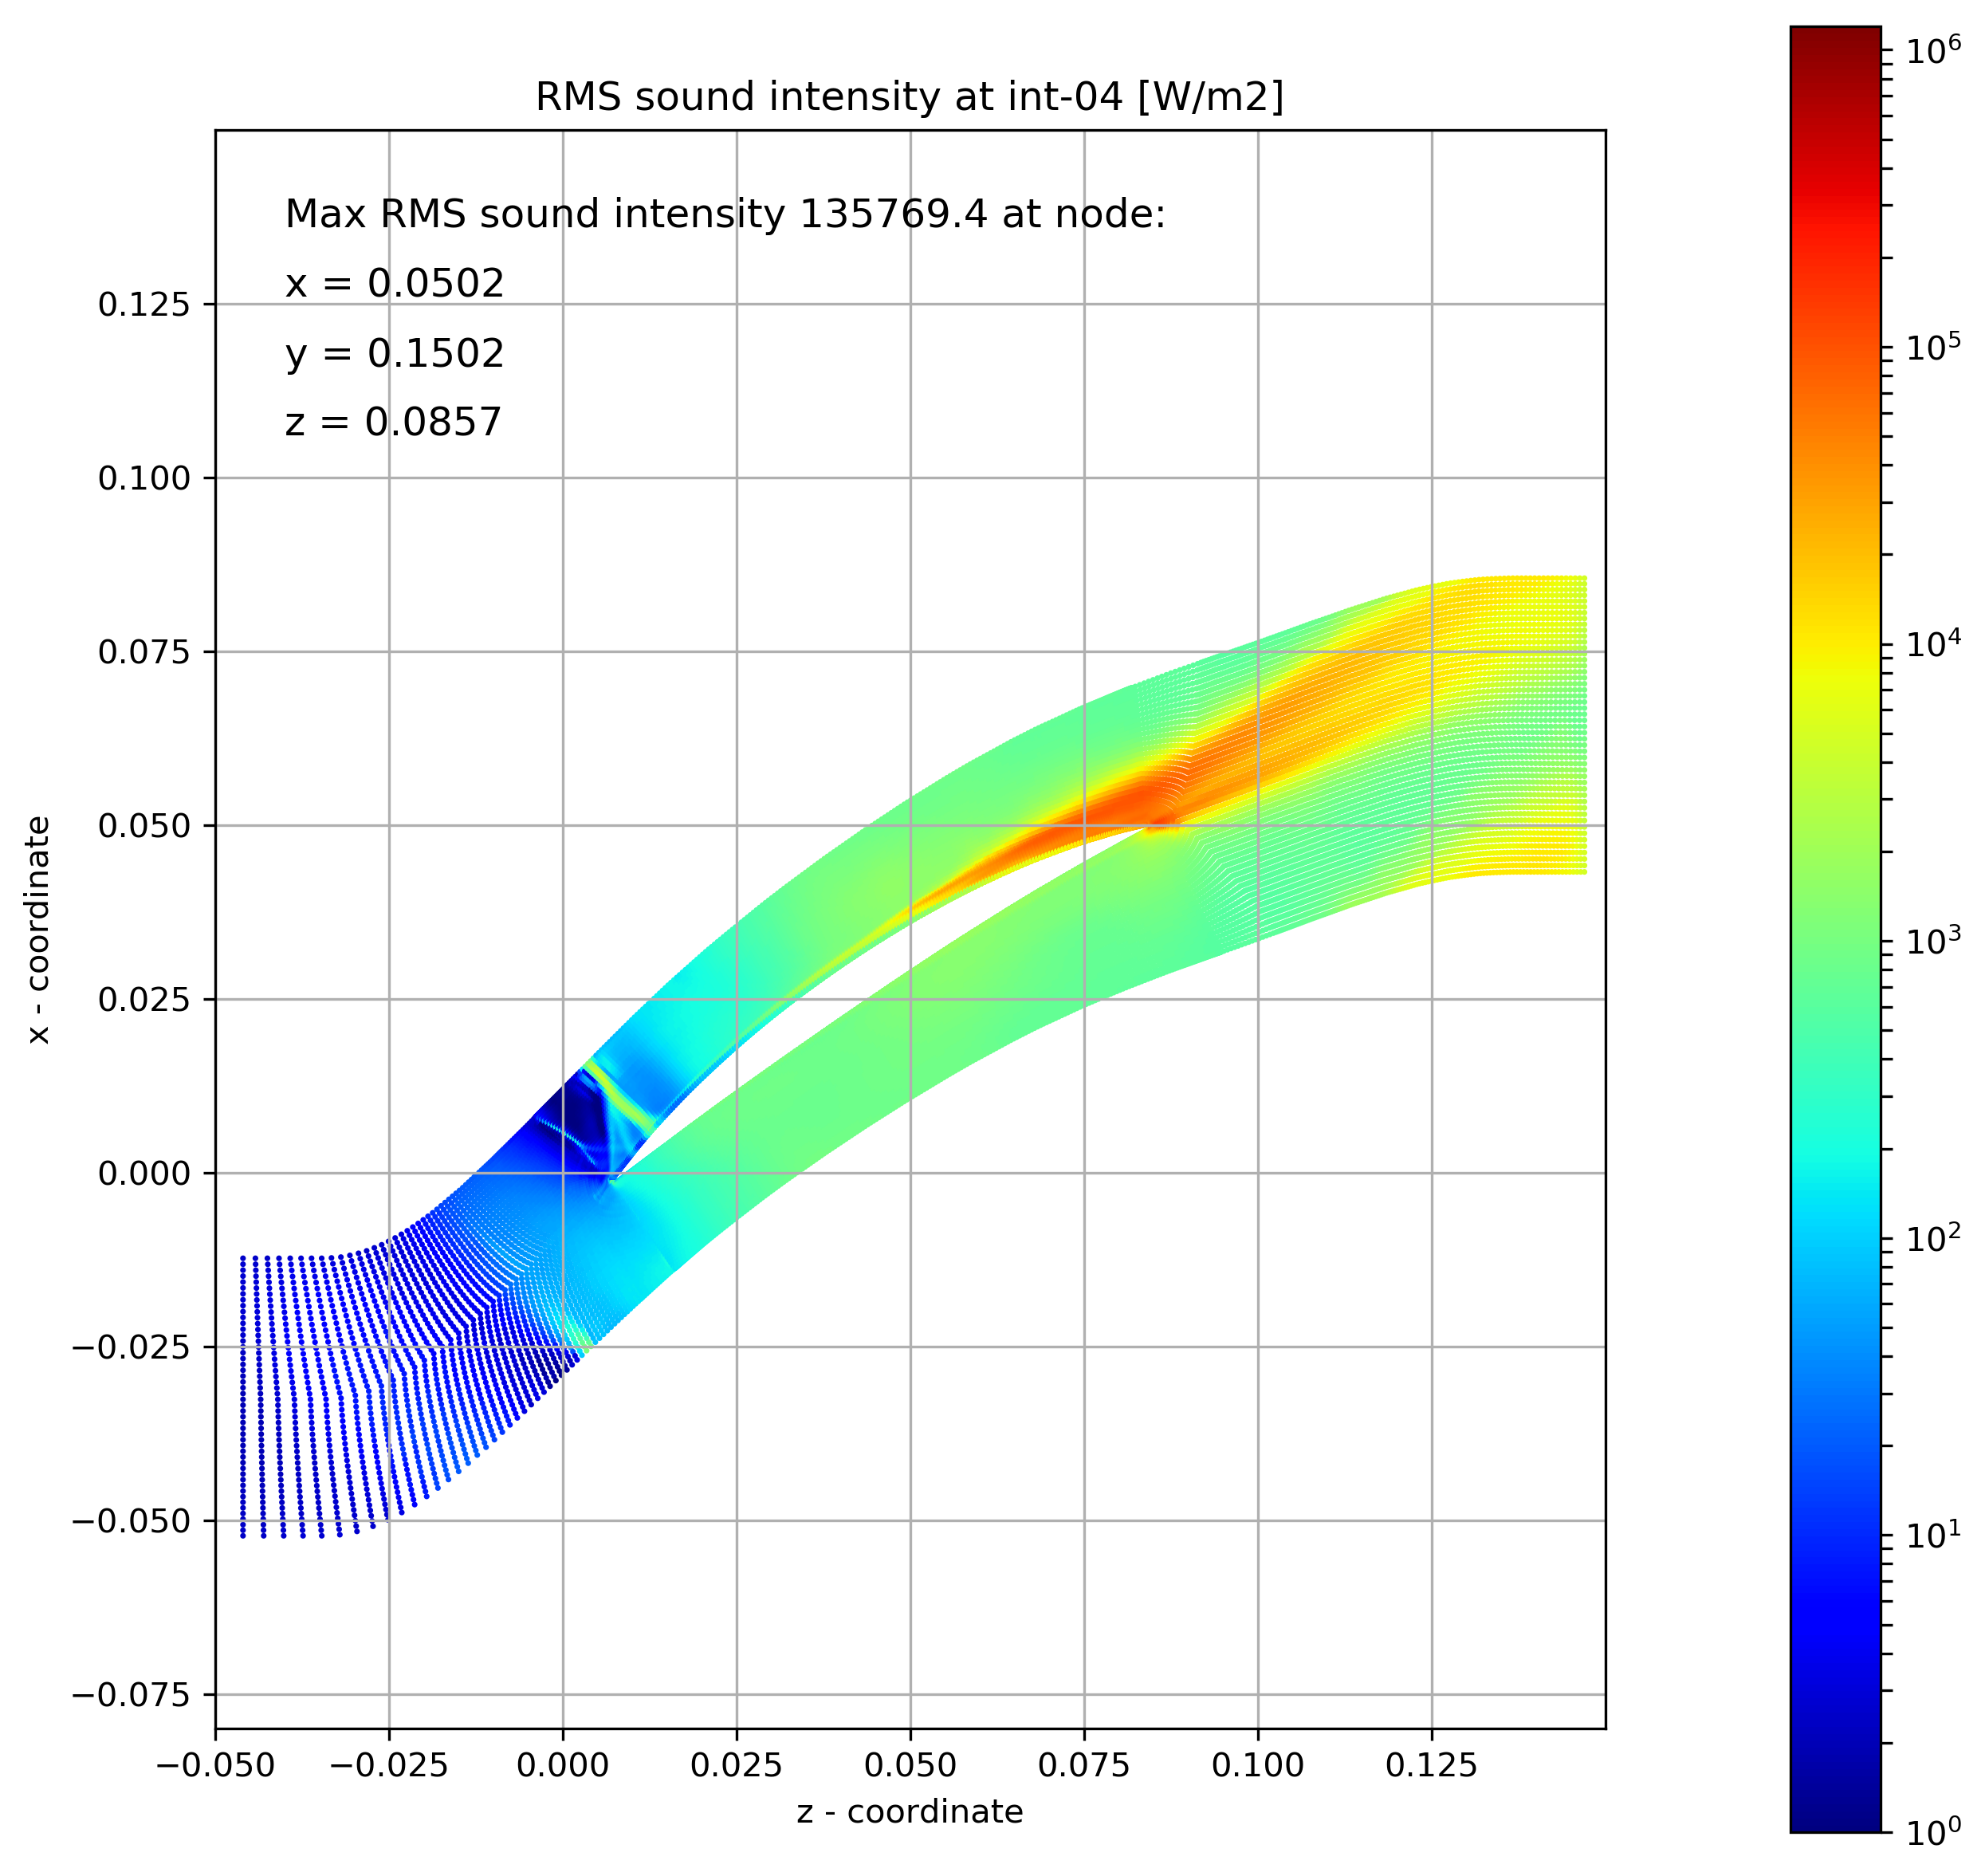
\includegraphics[width=0.75\textwidth]{Figures/int-04-rms-sil.png}
  \caption{RMS Sound intensity at int-04 mark} \label{int-04-rms-sil}
  
  \vspace*{\floatsep}% https://tex.stackexchange.com/q/26521/5764

  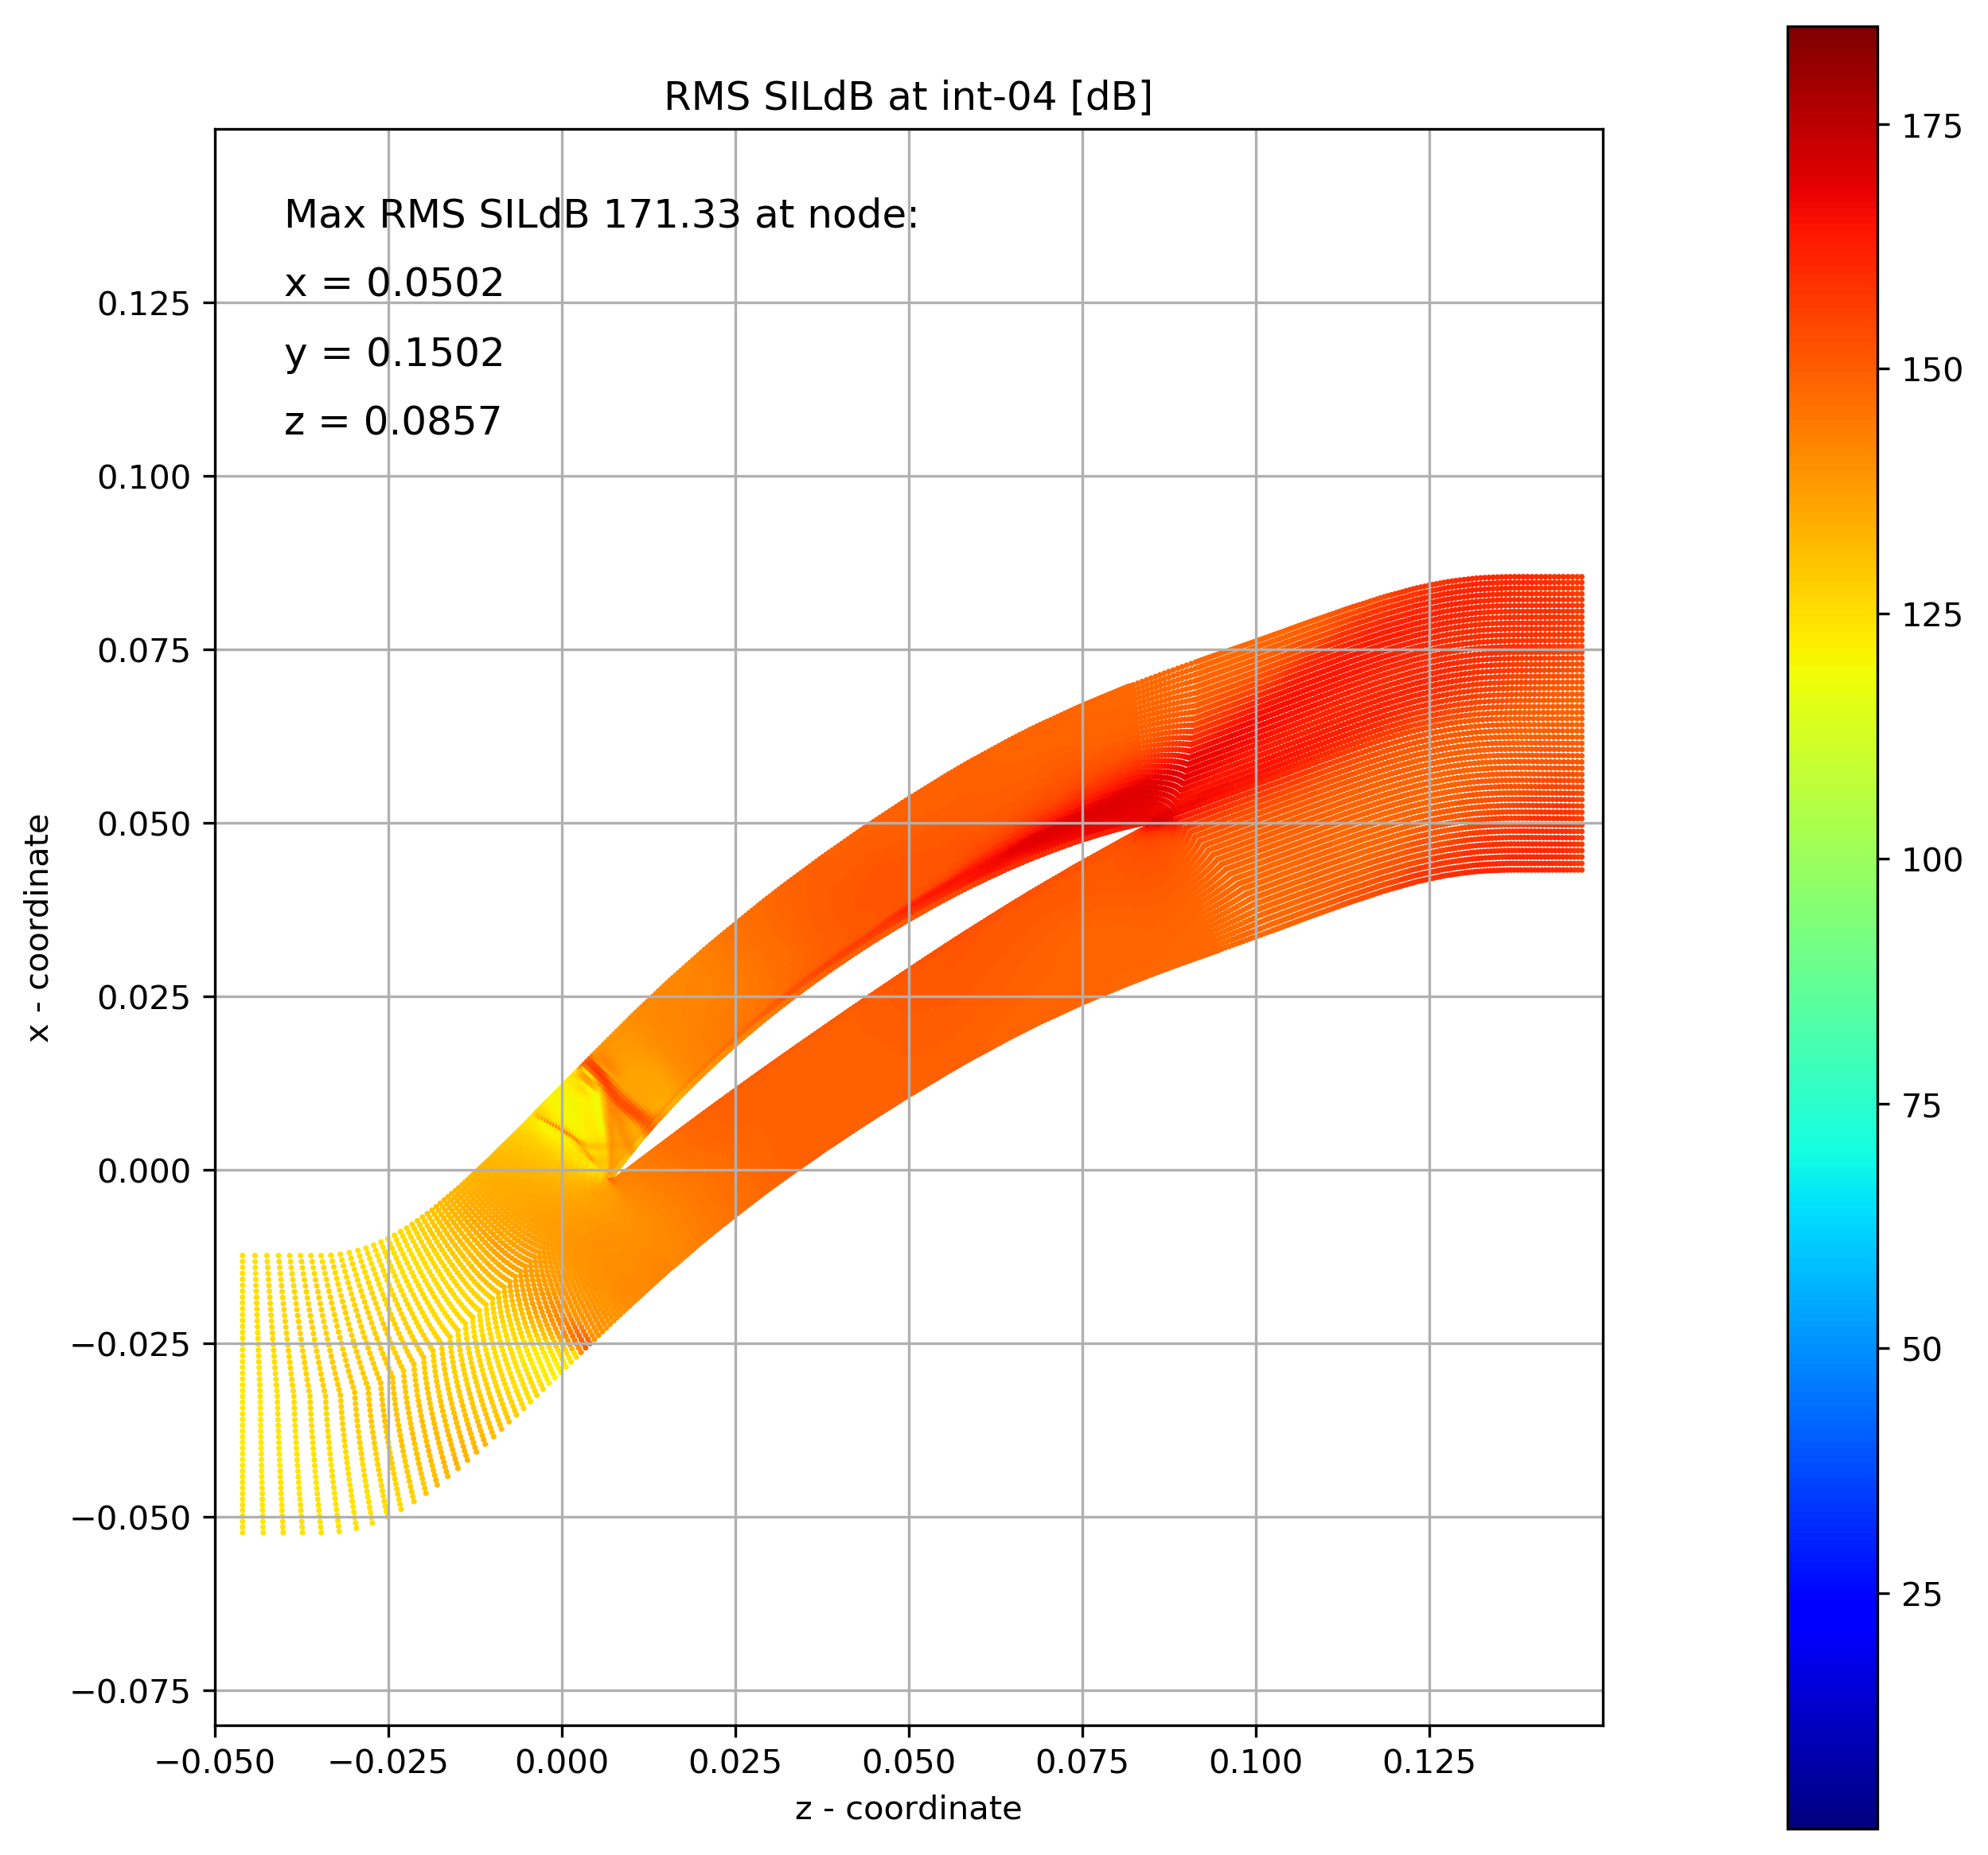
\includegraphics[width=0.75\textwidth]{Figures/int-04-rms-sildb.png}
  \caption{RMS Sound intensity decibel level at int-04 mark} \label{int-04-rms-sildb}
\end{figure}

%int-05
\begin{figure}[ht]
  \centering
  \includegraphics[width=0.75\textwidth]{Figures/int-05-rms-spl.png}
  \caption{RMS Sound pressure at int-05 mark} \label{int-05-rms-spl}
  
  \vspace*{\floatsep}% https://tex.stackexchange.com/q/26521/5764

  \includegraphics[width=0.75\textwidth]{Figures/int-05-rms-spldb.png}
  \caption{RMS Sound pressure decibel level at int-05 mark} \label{int-05-rms-spldb}
\end{figure}
%int-05
\begin{figure}[ht]
  \centering
  \includegraphics[width=0.75\textwidth]{Figures/int-05-rms-sil.png}
  \caption{RMS Sound intensity at int-05 mark} \label{int-05-rms-sil}
  
  \vspace*{\floatsep}% https://tex.stackexchange.com/q/26521/5764

  \includegraphics[width=0.75\textwidth]{Figures/int-05-rms-sildb.png}
  \caption{RMS Sound intensity decibel level at int-05 mark} \label{int-05-rms-sildb}
\end{figure}


%int-06
\begin{figure}[ht]
  \centering
  \includegraphics[width=0.75\textwidth]{Figures/int-06-rms-spl.png}
  \caption{RMS Sound pressure at int-06 mark} \label{int-06-rms-spl}
  
  \vspace*{\floatsep}% https://tex.stackexchange.com/q/26521/5764

  \includegraphics[width=0.75\textwidth]{Figures/int-06-rms-spldb.png}
  \caption{RMS Sound pressure decibel level at int-06 mark} \label{int-06-rms-spldb}
\end{figure}
%int-06
\begin{figure}[ht]
  \centering
  \includegraphics[width=0.75\textwidth]{Figures/int-06-rms-sil.png}
  \caption{RMS Sound intensity at int-06 mark} \label{int-06-rms-sil}
  
  \vspace*{\floatsep}% https://tex.stackexchange.com/q/26521/5764

  \includegraphics[width=0.75\textwidth]{Figures/int-06-rms-sildb.png}
  \caption{RMS Sound intensity decibel level at int-06 mark} \label{int-06-rms-sildb}
\end{figure}


%int-07
\begin{figure}[ht]
  \centering
  \includegraphics[width=0.75\textwidth]{Figures/int-07-rms-spl.png}
  \caption{RMS Sound pressure at int-07 mark} \label{int-07-rms-spl}
  
  \vspace*{\floatsep}% https://tex.stackexchange.com/q/26521/5764

  \includegraphics[width=0.75\textwidth]{Figures/int-07-rms-spldb.png}
  \caption{RMS Sound pressure decibel level at int-07 mark} \label{int-07-rms-spldb}
\end{figure}
%int-07
\begin{figure}[ht]
  \centering
  \includegraphics[width=0.75\textwidth]{Figures/int-07-rms-sil.png}
  \caption{RMS Sound intensity at int-07 mark} \label{int-07-rms-sil}
  
  \vspace*{\floatsep}% https://tex.stackexchange.com/q/26521/5764

  \includegraphics[width=0.75\textwidth]{Figures/int-07-rms-sildb.png}
  \caption{RMS Sound intensity decibel level at int-07 mark} \label{int-07-rms-sildb}
\end{figure}


%int-08
\begin{figure}[ht]
  \centering
  \includegraphics[width=0.75\textwidth]{Figures/int-08-rms-spl.png}
  \caption{RMS Sound pressure at int-08 mark} \label{int-08-rms-spl}
  
  \vspace*{\floatsep}% https://tex.stackexchange.com/q/26521/5764

  \includegraphics[width=0.75\textwidth]{Figures/int-08-rms-spldb.png}
  \caption{RMS Sound pressure decibel level at int-08 mark} \label{int-08-rms-spldb}
\end{figure}
%int-08
\begin{figure}[ht]
  \centering
  \includegraphics[width=0.75\textwidth]{Figures/int-08-rms-sil.png}
  \caption{RMS Sound intensity at int-08 mark} \label{int-08-rms-sil}
  
  \vspace*{\floatsep}% https://tex.stackexchange.com/q/26521/5764

  \includegraphics[width=0.75\textwidth]{Figures/int-08-rms-sildb.png}
  \caption{RMS Sound intensity decibel level at int-08 mark} \label{int-08-rms-sildb}
\end{figure}


%int-09
\begin{figure}[ht]
  \centering
  \includegraphics[width=0.75\textwidth]{Figures/int-09-rms-spl.png}
  \caption{RMS Sound pressure at int-09 mark} \label{int-09-rms-spl}
  
  \vspace*{\floatsep}% https://tex.stackexchange.com/q/26521/5764

  \includegraphics[width=0.75\textwidth]{Figures/int-09-rms-spldb.png}
  \caption{RMS Sound pressure decibel level at int-09 mark} \label{int-09-rms-spldb}
\end{figure}
%int-09
\begin{figure}[ht]
  \centering
  \includegraphics[width=0.75\textwidth]{Figures/int-09-rms-sil.png}
  \caption{RMS Sound intensity at int-09 mark} \label{int-09-rms-sil}
  
  \vspace*{\floatsep}% https://tex.stackexchange.com/q/26521/5764

  \includegraphics[width=0.75\textwidth]{Figures/int-09-rms-sildb.png}
  \caption{RMS Sound intensity decibel level at int-09 mark} \label{int-09-rms-sildb}
\end{figure}


%int-10
\begin{figure}[ht]
  \centering
  \includegraphics[width=0.75\textwidth]{Figures/int-10-rms-spl.png}
  \caption{RMS Sound pressure at int-10 mark} \label{int-10-rms-spl}
  
  \vspace*{\floatsep}% https://tex.stackexchange.com/q/26521/5764

  \includegraphics[width=0.75\textwidth]{Figures/int-10-rms-spldb.png}
  \caption{RMS Sound pressure decibel level at int-10 mark} \label{int-10-rms-spldb}
\end{figure}
%int-10
\begin{figure}[ht]
  \centering
  \includegraphics[width=0.75\textwidth]{Figures/int-10-rms-sil.png}
  \caption{RMS Sound intensity at int-10 mark} \label{int-10-rms-sil}
  
  \vspace*{\floatsep}% https://tex.stackexchange.com/q/26521/5764

  \includegraphics[width=0.75\textwidth]{Figures/int-10-rms-sildb.png}
  \caption{RMS Sound intensity decibel level at int-10 mark} \label{int-10-rms-sildb}
\end{figure}


%int-11
\begin{figure}[ht]
  \centering
  \includegraphics[width=0.75\textwidth]{Figures/int-11-rms-spl.png}
  \caption{RMS Sound pressure at int-11 mark} \label{int-11-rms-spl}
  
  \vspace*{\floatsep}% https://tex.stackexchange.com/q/26521/5764

  \includegraphics[width=0.75\textwidth]{Figures/int-11-rms-spldb.png}
  \caption{RMS Sound pressure decibel level at int-11 mark} \label{int-11-rms-spldb}
\end{figure}
%int-11
\begin{figure}[ht]
  \centering
  \includegraphics[width=0.75\textwidth]{Figures/int-11-rms-sil.png} 
  \caption{RMS Sound intensity at int-11 mark} \label{int-11-rms-sil}
  
  \vspace*{\floatsep}% https://tex.stackexchange.com/q/26521/5764

  \includegraphics[width=0.75\textwidth]{Figures/int-11-rms-sildb.png} 
  \caption{RMS Sound intensity decibel level at int-11 mark} \label{int-11-rms-sildb}
\end{figure}


%int-12
\begin{figure}[ht]
  \centering
  \includegraphics[width=0.75\textwidth]{Figures/int-12-rms-spl.png} 
  \caption{RMS Sound pressure at int-12 mark} \label{int-12-rms-spl}
  
  \vspace*{\floatsep}% https://tex.stackexchange.com/q/26521/5764

  \includegraphics[width=0.75\textwidth]{Figures/int-12-rms-spldb.png} 
  \caption{RMS Sound pressure decibel level at int-12 mark} \label{int-12-rms-spldb}
\end{figure}
%int-12
\begin{figure}[ht]
  \centering
  \includegraphics[width=0.75\textwidth]{Figures/int-12-rms-sil.png} 
  \caption{RMS Sound intensity at int-12 mark} \label{int-12-rms-sil}
  
  \vspace*{\floatsep}% https://tex.stackexchange.com/q/26521/5764

  \includegraphics[width=0.75\textwidth]{Figures/int-12-rms-sildb.png} 
  \caption{RMS Sound intensity decibel level at int-12 mark} \label{int-12-rms-sildb}
\end{figure}


%int-tip
\begin{figure}[ht]
  \centering
  \includegraphics[width=0.75\textwidth]{Figures/int-tip-rms-spl.png} 
  \caption{RMS Sound pressure at int-tip mark} \label{int-tip-rms-spl}
  
  \vspace*{\floatsep}% https://tex.stackexchange.com/q/26521/5764

  \includegraphics[width=0.75\textwidth]{Figures/int-tip-rms-spldb.png} 
  \caption{RMS Sound pressure decibel level at int-tip mark} \label{int-tip-rms-spldb}
\end{figure}
%int-12
\begin{figure}[ht]
  \centering
  \includegraphics[width=0.75\textwidth]{Figures/int-tip-rms-sil.png} 
  \caption{RMS Sound intensity at int-tip mark} \label{int-tip-rms-sil}
  
  \vspace*{\floatsep}% https://tex.stackexchange.com/q/26521/5764

  \includegraphics[width=0.75\textwidth]{Figures/int-tip-rms-sildb.png} 
  \caption{RMS Sound intensity decibel level at int-tip mark} \label{int-tip-rms-sildb}
\end{figure}
%% Appendix Template

\chapter{FFT plots} % Main appendix title

\label{fft_results} % Change X to a consecutive letter; for referencing this appendix elsewhere, use \ref{AppendixX}

\fancyhead[RE, LO]{\emph{FFT plots}} % Change X to a consecutive letter; this is for the header on each page - perhaps a shortened title

\begin{figure}[ht]
	\centering
	\includegraphics[width=0.9\textwidth]{Figures/blade-awf.png}
    \caption{Blade surface amplitude weighted average frequency [dB]} \label{blade-awaf}
\end{figure}	

\begin{figure}[ht]
	\centering
	\includegraphics[width=0.9\textwidth]{Figures/blade-peak-freq.png}
	\caption{Blade surface frequency of peak amplitude[Hz]} \label{blade-peak-freq}
\end{figure}

\begin{figure}[ht]
	\centering
	\includegraphics[width=0.9\textwidth]{Figures/blade-peak-mag.png}
	\caption{Blade surface peak amplitude [dB]} \label{blade-peak-mag}
\end{figure}

%int-01
\begin{figure}[ht]
  \centering
  \includegraphics[width=0.75\textwidth]{Figures/int-01_spectrum.png}
  \caption{Spectrum plot at int-01 mark} \label{int-01-spectrum}
  
  \vspace*{\floatsep}% https://tex.stackexchange.com/q/26521/5764

  \includegraphics[width=0.75\textwidth]{Figures/int-01-awaf.png}
  \caption{Amplitude weighted average frequency at int-01 mark} \label{int-01-awaf}
\end{figure}
%int-01
\begin{figure}[ht]
  \centering
  \includegraphics[width=0.75\textwidth]{Figures/int-01-peak-freq.png}
  \caption{Peak amplitude frequency int-01 mark} \label{int-01-peak-freq}
  
  \vspace*{\floatsep}% https://tex.stackexchange.com/q/26521/5764

  \includegraphics[width=0.75\textwidth]{Figures/int-01-peak-mag.png}
  \caption{Peak magnitude at int-01 mark} \label{int-01-peak-mag}
\end{figure}

%int-02
\begin{figure}[ht]
  \centering
  \includegraphics[width=0.75\textwidth]{Figures/int-02_spectrum.png}
  \caption{Spectrum plot at int-02 mark} \label{int-02-spectrum}
  
  \vspace*{\floatsep}% https://tex.stackexchange.com/q/26521/5764

  \includegraphics[width=0.75\textwidth]{Figures/int-02-awaf.png}
  \caption{Amplitude weighted average frequency at int-02 mark} \label{int-02-awaf}
\end{figure}
%int-02
\begin{figure}[ht]
  \centering
  \includegraphics[width=0.75\textwidth]{Figures/int-02-peak-freq.png}
  \caption{Peak amplitude frequency int-02 mark} \label{int-02-peak-freq}
  
  \vspace*{\floatsep}% https://tex.stackexchange.com/q/26521/5764

  \includegraphics[width=0.75\textwidth]{Figures/int-02-peak-mag.png}
  \caption{Peak magnitude at int-02 mark} \label{int-02-peak-mag}
\end{figure}

%int-03
\begin{figure}[ht]
  \centering
  \includegraphics[width=0.75\textwidth]{Figures/int-03_spectrum.png}
  \caption{Spectrum plot at int-03 mark} \label{int-03-spectrum}
  
  \vspace*{\floatsep}% https://tex.stackexchange.com/q/26521/5764

  \includegraphics[width=0.75\textwidth]{Figures/int-03-awaf.png}
  \caption{Amplitude weighted average frequency at int-03 mark} \label{int-03-awaf}
\end{figure}
%int-03
\begin{figure}[ht]
  \centering
  \includegraphics[width=0.75\textwidth]{Figures/int-03-peak-freq.png}
  \caption{Peak amplitude frequency int-03 mark} \label{int-03-peak-freq}
  
  \vspace*{\floatsep}% https://tex.stackexchange.com/q/26521/5764

  \includegraphics[width=0.75\textwidth]{Figures/int-03-peak-mag.png}
  \caption{Peak magnitude at int-03 mark} \label{int-03-peak-mag}
\end{figure}

%int-04
\begin{figure}[ht]
  \centering
  \includegraphics[width=0.75\textwidth]{Figures/int-04_spectrum.png}
  \caption{Spectrum plot at int-04 mark} \label{int-04-spectrum}
  
  \vspace*{\floatsep}% https://tex.stackexchange.com/q/26521/5764

  \includegraphics[width=0.75\textwidth]{Figures/int-04-awaf.png}
  \caption{Amplitude weighted average frequency at int-04 mark} \label{int-04-awaf}
\end{figure}
%int-04
\begin{figure}[ht]
  \centering
  \includegraphics[width=0.75\textwidth]{Figures/int-04-peak-freq.png}
  \caption{Peak amplitude frequency int-04 mark} \label{int-04-peak-freq}
  
  \vspace*{\floatsep}% https://tex.stackexchange.com/q/26521/5764

  \includegraphics[width=0.75\textwidth]{Figures/int-04-peak-mag.png}
  \caption{Peak magnitude at int-04 mark} \label{int-04-peak-mag}
\end{figure}

%int-05
\begin{figure}[ht]
  \centering
  \includegraphics[width=0.75\textwidth]{Figures/int-05_spectrum.png}
  \caption{Spectrum plot at int-05 mark} \label{int-05-spectrum}
  
  \vspace*{\floatsep}% https://tex.stackexchange.com/q/26521/5764

  \includegraphics[width=0.75\textwidth]{Figures/int-05-awaf.png}
  \caption{Amplitude weighted average frequency at int-05 mark} \label{int-05-awaf}
\end{figure}
%int-05
\begin{figure}[ht]
  \centering
  \includegraphics[width=0.75\textwidth]{Figures/int-05-peak-freq.png}
  \caption{Peak amplitude frequency int-05 mark} \label{int-05-peak-freq}
  
  \vspace*{\floatsep}% https://tex.stackexchange.com/q/26521/5764

  \includegraphics[width=0.75\textwidth]{Figures/int-05-peak-mag.png}
  \caption{Peak magnitude at int-05 mark} \label{int-05-peak-mag}
\end{figure}

%int-06
\begin{figure}[ht]
  \centering
  \includegraphics[width=0.75\textwidth]{Figures/int-06_spectrum.png}
  \caption{Spectrum plot at int-06 mark} \label{int-06-spectrum}
  
  \vspace*{\floatsep}% https://tex.stackexchange.com/q/26521/5764

  \includegraphics[width=0.75\textwidth]{Figures/int-06-awaf.png}
  \caption{Amplitude weighted average frequency at int-06 mark} \label{int-06-awaf}
\end{figure}
%int-06
\begin{figure}[ht]
  \centering
  \includegraphics[width=0.75\textwidth]{Figures/int-06-peak-freq.png}
  \caption{Peak amplitude frequency int-06 mark} \label{int-06-peak-freq}
  
  \vspace*{\floatsep}% https://tex.stackexchange.com/q/26521/5764

  \includegraphics[width=0.75\textwidth]{Figures/int-06-peak-mag.png}
  \caption{Peak magnitude at int-06 mark} \label{int-06-peak-mag}
\end{figure}

%int-07
\begin{figure}[ht]
  \centering
  \includegraphics[width=0.75\textwidth]{Figures/int-07_spectrum.png}
  \caption{Spectrum plot at int-07 mark} \label{int-07-spectrum}
  
  \vspace*{\floatsep}% https://tex.stackexchange.com/q/26521/5764

  \includegraphics[width=0.75\textwidth]{Figures/int-07-awaf.png}
  \caption{Amplitude weighted average frequency at int-07 mark} \label{int-07-awaf}
\end{figure}
%int-07
\begin{figure}[ht]
  \centering
  \includegraphics[width=0.75\textwidth]{Figures/int-07-peak-freq.png}
  \caption{Peak amplitude frequency int-07 mark} \label{int-07-peak-freq}
  
  \vspace*{\floatsep}% https://tex.stackexchange.com/q/26521/5764

  \includegraphics[width=0.75\textwidth]{Figures/int-07-peak-mag.png}
  \caption{Peak magnitude at int-07 mark} \label{int-07-peak-mag}
\end{figure}

%int-08
\begin{figure}[ht]
  \centering
  \includegraphics[width=0.75\textwidth]{Figures/int-08_spectrum.png}
  \caption{Spectrum plot at int-08 mark} \label{int-08-spectrum}
  
  \vspace*{\floatsep}% https://tex.stackexchange.com/q/26521/5764

  \includegraphics[width=0.75\textwidth]{Figures/int-08-awaf.png}
  \caption{Amplitude weighted average frequency at int-08 mark} \label{int-08-awaf}
\end{figure}
%int-08
\begin{figure}[ht]
  \centering
  \includegraphics[width=0.75\textwidth]{Figures/int-08-peak-freq.png}
  \caption{Peak amplitude frequency int-08 mark} \label{int-08-peak-freq}
  
  \vspace*{\floatsep}% https://tex.stackexchange.com/q/26521/5764

  \includegraphics[width=0.75\textwidth]{Figures/int-08-peak-mag.png}
  \caption{Peak magnitude at int-08 mark} \label{int-08-peak-mag}
\end{figure}

%int-09
\begin{figure}[ht]
  \centering
  \includegraphics[width=0.75\textwidth]{Figures/int-09_spectrum.png}
  \caption{Spectrum plot at int-09 mark} \label{int-09-spectrum}
  
  \vspace*{\floatsep}% https://tex.stackexchange.com/q/26521/5764

  \includegraphics[width=0.75\textwidth]{Figures/int-09-awaf.png}
  \caption{Amplitude weighted average frequency at int-09 mark} \label{int-09-awaf}
\end{figure}
%int-09
\begin{figure}[ht]
  \centering
  \includegraphics[width=0.75\textwidth]{Figures/int-09-peak-freq.png}
  \caption{Peak amplitude frequency int-09 mark} \label{int-09-peak-freq}
  
  \vspace*{\floatsep}% https://tex.stackexchange.com/q/26521/5764

  \includegraphics[width=0.75\textwidth]{Figures/int-09-peak-mag.png}
  \caption{Peak magnitude at int-09 mark} \label{int-09-peak-mag}
\end{figure}

%int-10
\begin{figure}[ht]
  \centering
  \includegraphics[width=0.75\textwidth]{Figures/int-10_spectrum.png}
  \caption{Spectrum plot at int-10 mark} \label{int-10-spectrum}
  
  \vspace*{\floatsep}% https://tex.stackexchange.com/q/26521/5764

  \includegraphics[width=0.75\textwidth]{Figures/int-10-awaf.png}
  \caption{Amplitude weighted average frequency at int-10 mark} \label{int-10-awaf}
\end{figure}
%int-10
\begin{figure}[ht]
  \centering
  \includegraphics[width=0.75\textwidth]{Figures/int-10-peak-freq.png}
  \caption{Peak amplitude frequency int-10 mark} \label{int-10-peak-freq}
  
  \vspace*{\floatsep}% https://tex.stackexchange.com/q/26521/5764

  \includegraphics[width=0.75\textwidth]{Figures/int-10-peak-mag.png}
  \caption{Peak magnitude at int-10 mark} \label{int-10-peak-mag}
\end{figure}

%int-11
\begin{figure}[ht]
  \centering
  \includegraphics[width=0.75\textwidth]{Figures/int-11_spectrum.png}
  \caption{Spectrum plot at int-11 mark} \label{int-11-spectrum}
  
  \vspace*{\floatsep}% https://tex.stackexchange.com/q/26521/5764

  \includegraphics[width=0.75\textwidth]{Figures/int-11-awaf.png}
  \caption{Amplitude weighted average frequency at int-11 mark} \label{int-11-awaf}
\end{figure}
%int-11
\begin{figure}[ht]
  \centering
  \includegraphics[width=0.75\textwidth]{Figures/int-11-peak-freq.png}
  \caption{Peak amplitude frequency int-11 mark} \label{int-11-peak-freq}
  
  \vspace*{\floatsep}% https://tex.stackexchange.com/q/26521/5764

  \includegraphics[width=0.75\textwidth]{Figures/int-11-peak-mag.png}
  \caption{Peak magnitude at int-11 mark} \label{int-11-peak-mag}
\end{figure}

%int-12
\begin{figure}[ht]
  \centering
  \includegraphics[width=0.75\textwidth]{Figures/int-12_spectrum.png}
  \caption{Spectrum plot at int-12 mark} \label{int-12-spectrum}
  
  \vspace*{\floatsep}% https://tex.stackexchange.com/q/26521/5764

  \includegraphics[width=0.75\textwidth]{Figures/int-12-awaf.png}
  \caption{Amplitude weighted average frequency at int-12 mark} \label{int-12-awaf}
\end{figure}
%int-12
\begin{figure}[ht]
  \centering
  \includegraphics[width=0.75\textwidth]{Figures/int-12-peak-freq.png}
  \caption{Peak amplitude frequency int-12 mark} \label{int-12-peak-freq}
  
  \vspace*{\floatsep}% https://tex.stackexchange.com/q/26521/5764

  \includegraphics[width=0.75\textwidth]{Figures/int-12-peak-mag.png}
  \caption{Peak magnitude at int-12 mark} \label{int-12-peak-mag}
\end{figure}

%int-tip
\begin{figure}[ht]
  \centering
  \includegraphics[width=0.75\textwidth]{Figures/int-tip_spectrum.png}
  \caption{Spectrum plot at int-tip mark} \label{int-tip-spectrum}
  
  \vspace*{\floatsep}% https://tex.stackexchange.com/q/26521/5764

  \includegraphics[width=0.75\textwidth]{Figures/int-tip-awaf.png}
  \caption{Amplitude weighted average frequency at int-tip mark} \label{int-tip-awaf}
\end{figure}
%int-tip
\begin{figure}[ht]
  \centering
  \includegraphics[width=0.75\textwidth]{Figures/int-tip-peak-freq.png}
  \caption{Peak amplitude frequency int-tip mark} \label{int-tip-peak-freq}
  
  \vspace*{\floatsep}% https://tex.stackexchange.com/q/26521/5764

  \includegraphics[width=0.75\textwidth]{Figures/int-tip-peak-mag.png}
  \caption{Peak magnitude at int-tip mark} \label{int-tip-peak-mag}
\end{figure}
%% Appendix Template

\chapter{CFD validation} % Main appendix title

\label{cfd_results} % Change X to a consecutive letter; for referencing this appendix elsewhere, use \ref{AppendixX}
\lhead{\emph{CFD validation}} % Change X to a consecutive letter; this is for the header on each page - perhaps a shortened title

Here will be validation

\begin{figure}[ht]
    \centering
	\includegraphics[width=0.9\textwidth]{Pictures/kitten-placeholder.jpg}
    \caption{Plot} \label{dupa}
\end{figure}
%\chapter{Code for direct formulation of noise analysis} % Main appendix title

\label{codedirect} % For referencing this appendix elsewhere, use \ref{AppendixA}

\lhead{\emph{Code for direct formulation of noise analysis}} % This is for the header on each page - perhaps a shortened title

\begin{lstlisting}[language=Python]
# dask-noise.py
print("Loading Libraries...")
import os, sys
import csv
import platform
import numpy as np
import pandas as pd
import dask.dataframe as dd
import math
print("Loaded Libraries...")
print("Starting code...")
print("Loading directories..")
path_data = './flow-data/<folder_name>'
path_acu = './noise-data/<folder_name>/acu'
print("Loaded directories...")
print("Loading batch data...")
os.chdir(path_data)
batch_data = dd.read_csv('*.dat', delimiter=r"\s+", decimal='.')
print("Batch data done...")
print("Calculating batch averages...")
averages = pd.DataFrame(batch_data.groupby('nodenumber').mean().compute())
print("Batch averages done...")
print("Generating average pressure dataframe")
avg_static_p = pd.DataFrame({'pressure': averages['pressure']})
print("Generating average velocity dataframe")
avg_rel_v = pd.DataFrame(
		{'rel-velocity-magnitude': averages['rel-velocity-magnitude']})
print("Generating node coordinates...")
node_coords = pd.DataFrame({
    'x-coordinate': averages['x-coordinate'],
    'y-coordinate': averages['y-coordinate'],
    'z-coordinate': averages['z-coordinate']
})
del(batch_data)
print("Batch data deleted...")
print("Listing files...")
filelist = sorted(os.listdir(path_data))[len(os.listdir(path_acu)):]
print("Starting noise analysis loop...")
for file in filelist:
    os.chdir(path_data)
    timestep = str(os.path.basename(str(file)))[7:-4]
    time_static_p = pd.DataFrame(pd.read_csv(file, delimiter=r"\s+"))
    	.set_index('nodenumber')
    acoustic_p = time_static_p.subtract(avg_static_p, fill_value=None)
    spl_db = acoustic_p.apply(lambda x: 20 * np.log10(np.abs(x)/0.00002), axis=1)
    time_rel_vel = pd.DataFrame(pd.read_csv(file, delimiter=r"\s+"))
    	.set_index('nodenumber')
    particle_v = time_rel_vel.subtract(avg_rel_v, fill_value=None).abs()
    sound_intensity = pd.DataFrame(
    	acoustic_p.values*particle_v.values,
    	index=acoustic_p.index)
    sil_db = sound_intensity.apply(
    	lambda x: 10 * np.log10(np.abs(x)/1e-12), axis=1)
    acoustic_data = pd.concat(
    	[node_coords,
    	acoustic_p,
    	spl_db,
    	particle_v,
    	sound_intensity,
    	sil_db], axis=1)
    acoustic_data.columns =
    	['x-coordinate',
    	'y-coordinate',
    	'z-coordinate',
    	'sound-pressure',
    	'spl-db',
    	'particle-velocity',
    	'sound-intensity',
    	'sil-db']
    os.chdir(path_acu)
    acoustic_data.to_csv(str('<filename>_' + str(timestep) + '.dat'), sep=',')
    print(str('<filename>' + str(timestep) + '.dat done...'))
print("Exiting noise analysis loop...")
print("Script done, exiting.")
\end{lstlisting}
%\chapter{Folder Structure} % Main appendix title

\label{folders} % For referencing this appendix elsewhere, use \ref{AppendixA}

\lhead{\emph{Folder Structure}} % This is for the header on each page - perhaps a shortened title

\begin{forest}
  for tree={
    font=\ttfamily,
    grow'=0,
    child anchor=west,
    parent anchor=south,
    anchor=west,
    calign=first,
    edge path={
      \noexpand\path [draw, \forestoption{edge}]
      (!u.south west) +(7.5pt,0) |- node[fill,inner sep=1.25pt] {} (.child anchor)\forestoption{edge label};
    },
    before typesetting nodes={
      if n=1
        {insert before={[,phantom]}}
        {}
    },
    fit=band,
    before computing xy={l=15pt},
  }
[flow-data
	[int-01 ... int-tip]
	[lead, pside, sside, tip, trail]
]
\end{forest} \\
\\
\begin{forest}
  for tree={
    font=\ttfamily,
    grow'=0,
    child anchor=west,
    parent anchor=south,
    anchor=west,
    calign=first,
    edge path={
      \noexpand\path [draw, \forestoption{edge}]
      (!u.south west) +(7.5pt,0) |- node[fill,inner sep=1.25pt] {} (.child anchor)\forestoption{edge label};
    },
    before typesetting nodes={
      if n=1
        {insert before={[,phantom]}}
        {}
    },
    fit=band,
    before computing xy={l=15pt},
  }
[noise-data
	[int-01-post ... int-tip-post
		[acu]
		[plots]
	]
	[lead, pside, sside, tip, trail
		[...]	
	]
]
\end{forest} \\
\\
\begin{forest}
  for tree={
    font=\ttfamily,
    grow'=0,
    child anchor=west,
    parent anchor=south,
    anchor=west,
    calign=first,
    edge path={
      \noexpand\path [draw, \forestoption{edge}]
      (!u.south west) +(7.5pt,0) |- node[fill,inner sep=1.25pt] {} (.child anchor)\forestoption{edge label};
    },
    before typesetting nodes={
      if n=1
        {insert before={[,phantom]}}
        {}
    },
    fit=band,
    before computing xy={l=15pt},
  }
[results
	[coords]
	[fft]
	[rms]
]
\end{forest}
%\chapter{Code for RMS computation} % Main appendix title

\label{rms_code} % For referencing this appendix elsewhere, use \ref{AppendixA}

\fancyhead[RE, LO]{\emph{Code for RMS computation}} % This is for the header on each page - perhaps a shortened title
\begin{lstlisting}[language=Python]
#rms.py
print("Loading Libraries...")
import os
import csv
import platform
import numpy as np
from scipy.fftpack import fft
import pandas as pd
import dask.dataframe as dd
import math
import matplotlib.pyplot as plt
print("Loaded Libraries...")

#PLGRID
print("Loading directories..")
path_acu = './noise-data/<folder_name>/acu'
path_rms = './results/rms'
print("Loaded directories...")

print("Loading batch data...")
os.chdir(path_acu)
batch_data = dd.read_csv('*1.dat',
			delimiter=",",
			decimal='.',
			usecols=["nodenumber", "sound-pressure", "sound-intensity"])
batch_data = batch_data.set_index("nodenumber")
print("Batch data done...")

print("Calculating rms...")
rms = pd.DataFrame(batch_data.groupby('nodenumber').std().compute())
rms['rms_spldb'] = rms['sound-pressure'].apply(lambda x: 20*np.log10(x/0.00002))
rms['rms_sildb'] = rms['sound-intensity'].apply(lambda x: 10*np.log10(x/1e-12))

print("Saving...")
os.chdir(path_rms)
rms.to_csv(str('<filename>'), sep=",")
\end{lstlisting}
%\chapter{Code for discrete Fourier analysis} % Main appendix title

\label{codefft} % For referencing this appendix elsewhere, use \ref{AppendixA}

\lhead{\emph{Code for discrete Fourier analysis}} % This is for the header on each page - perhaps a shortened title

\begin{lstlisting}[language=Python]
#fft.py
print("Loading Libraries...")
import os
import csv
import platform
import numpy as np
from scipy.fftpack import fft
import pandas as pd
import dask.dataframe as dd
import math
print("Loaded Libraries...")
print("Starting code...")
print("Loading directories..")
path_acu = './noise-data/<folder_name>/acu'
path_fft = './results/fft'
print("Loaded directories...")
print("Loading batch data...")
os.chdir(path_acu)
batch_pressure = dd.read_csv('*.dat',
				delimiter=",",
				decimal='.',
				usecols=["nodenumber", "sound-pressure"])
batch_pressure = batch_pressure.set_index("nodenumber")
print("Batch data done...")
print("Calculating FFT...") 
batch_fft = batch_pressure.groupby('nodenumber').apply(
				lambda x: fft(x),
				meta=('node-fourier-series', 'f8')
				).compute()
print("FFT Done..") 
print("Saving FFT to dataframe...")
#node_fft_max.set_index('nodenumber')
os.chdir(path_fft)
batch_fft.to_csv(str('<file_name_fft>.dat'), sep=",")
print("Dataframe saved...")
print("Script completed...")
\end{lstlisting}
%\chapter{Blade design surface coordinates} % Main appendix title

\label{r67_coords_data} % For referencing this appendix elsewhere, use \ref{AppendixA}

\lhead{\emph{Blade design surface coordinates}} % This is for the header on each page - perhaps a shortened title

% Please add the following required packages to your document preamble:
% \usepackage{booktabs}
% \usepackage{graphicx}
\begin{table}[ht!]
\centering
\caption{int-00 coordinates}
\label{tab:int-00-coords}
\ttfamily
\resizebox{\textwidth}{!}{%
\begin{tabular}{@{}rrrrrrrr@{}}
\toprule
K  & Z       & THSP1\_X & THSP1\_Y  & THSP2\_X & THSP2\_Y  & THSPM\_X & THSPM\_Y  \\ \midrule
1  & 0.0000  & 0.74067  & 85.62460  & -0.15242 & 85.62766  & 0.29413  & 85.62729  \\
2  & 2.7160  & 3.11951  & 86.18426  & 1.39100  & 86.22948  & 2.25537  & 86.21120  \\
3  & 5.4378  & 5.37389  & 86.71885  & 2.91879  & 86.83616  & 4.14676  & 86.78619  \\
4  & 8.1570  & 7.46236  & 87.24062  & 4.35340  & 87.45091  & 5.90882  & 87.35960  \\
5  & 10.8754 & 9.38840  & 87.76236  & 5.60446  & 88.08499  & 7.49817  & 87.94403  \\
6  & 13.5921 & 11.25541 & 88.28179  & 6.79892  & 88.73632  & 9.03003  & 88.53710  \\
7  & 16.3072 & 13.03696 & 88.80698  & 7.98425  & 89.40299  & 10.51483 & 89.14079  \\
8  & 19.0194 & 14.62103 & 89.36128  & 9.09032  & 90.09205  & 11.86130 & 89.76927  \\
9  & 21.7294 & 16.06181 & 89.94555  & 10.12289 & 90.80590  & 13.09942 & 90.42450  \\
10 & 24.4372 & 17.40108 & 90.55801  & 11.10789 & 91.54325  & 14.26299 & 91.10498  \\
11 & 27.1419 & 18.63870 & 91.19793  & 12.05660 & 92.29898  & 15.35752 & 91.80746  \\
12 & 29.8434 & 19.77118 & 91.86337  & 12.95796 & 93.06917  & 16.37567 & 92.52900  \\
13 & 32.5408 & 20.80456 & 92.54873  & 13.80767 & 93.84799  & 17.31830 & 93.26400  \\
14 & 35.2334 & 21.74766 & 93.24722  & 14.60965 & 94.62855  & 18.19177 & 94.00566  \\
15 & 37.9207 & 22.60659 & 93.95188  & 15.36779 & 95.40359  & 19.00106 & 94.74689  \\
16 & 40.6023 & 23.37726 & 94.65824  & 16.08421 & 96.16640  & 19.74514 & 95.48198  \\
17 & 43.2773 & 24.06404 & 95.35947  & 16.75617 & 96.91097  & 20.42484 & 96.20464  \\
18 & 45.9453 & 24.66787 & 96.05004  & 17.38102 & 97.63203  & 21.03932 & 96.90955  \\
19 & 48.6060 & 25.18324 & 96.72676  & 17.95914 & 98.32462  & 21.58598 & 97.59256  \\
20 & 51.2594 & 25.61310 & 97.38664  & 18.48850 & 98.98668  & 22.06530 & 98.25126  \\
21 & 53.9054 & 25.95965 & 98.03052  & 18.96683 & 99.62001  & 22.47729 & 98.88710  \\
22 & 56.5443 & 26.21953 & 98.66096  & 19.39503 & 100.22616 & 22.82070 & 99.50208  \\
23 & 59.1761 & 26.39038 & 99.27984  & 19.77311 & 100.80656 & 23.09437 & 100.09790 \\
24 & 61.8010 & 26.47090 & 99.88845  & 20.09815 & 101.36309 & 23.29619 & 100.67621 \\
25 & 64.4192 & 26.45901 & 100.48859 & 20.36736 & 101.89802 & 23.42379 & 101.23913 \\
26 & 67.0311 & 26.34948 & 101.08182 & 20.57887 & 102.41259 & 23.47361 & 101.78811 \\
27 & 69.6369 & 26.13823 & 101.66972 & 20.72790 & 102.90915 & 23.44126 & 102.32520 \\
28 & 72.2368 & 25.82206 & 102.25274 & 20.81474 & 103.38834 & 23.32531 & 102.85102 \\
29 & 74.8312 & 25.39490 & 102.83242 & 20.83469 & 103.85241 & 23.12042 & 103.36756 \\
30 & 77.4204 & 24.85045 & 103.40908 & 20.78502 & 104.30228 & 22.82210 & 103.87557 \\
31 & 80.0045 & 24.17617 & 103.98423 & 20.65989 & 104.73956 & 22.42121 & 104.37670 \\
32 & 82.5840 & 23.37613 & 104.55498 & 20.45559 & 105.16537 & 21.91798 & 104.87034 \\
33 & 85.1592 & 22.43256 & 105.12306 & 20.15896 & 105.58264 & 21.29700 & 105.35899 \\
34 & 87.7309 & 21.28188 & 105.69777 & 19.74814 & 105.99504 & 20.51555 & 105.84918 \\
35 & 90.2991 & 19.94258 & 106.27120 & 19.24182 & 106.40032 & 19.59231 & 106.33634 \\ \bottomrule
\end{tabular}%
}
\end{table}
\vfill
\clearpage

% Please add the following required packages to your document preamble:
% \usepackage{booktabs}
% \usepackage{graphicx}
\begin{table}[ht!]
\centering
\caption{int-01 coordinates}
\label{tab:int-01-coords}
\ttfamily
\resizebox{\textwidth}{!}{%
\begin{tabular}{@{}rrrrrrrr@{}}
\toprule
K  & Z       & THSP1\_X & THSP1\_Y  & THSP2\_X & THSP2\_Y  & THSPM\_X & THSPM\_Y  \\ \midrule
1  & 0.0000  & 0.82717  & 95.62422  & -0.17022 & 95.62765  & 0.32848  & 95.62724  \\
2  & 2.7160  & 3.48123  & 96.17772  & 1.55230  & 96.22818  & 2.51689  & 96.20778  \\
3  & 5.4378  & 5.99240  & 96.69971  & 3.25473  & 96.83052  & 4.62403  & 96.77479  \\
4  & 8.1570  & 8.31463  & 97.20424  & 4.85059  & 97.43854  & 6.58365  & 97.33680  \\
5  & 10.8754 & 10.45209 & 97.70563  & 6.23944  & 98.06481  & 8.34769  & 97.90788  \\
6  & 13.5921 & 12.52011 & 98.20150  & 7.56288  & 98.70709  & 10.04468 & 98.48549  \\
7  & 16.3072 & 14.48941 & 98.70094  & 8.87377  & 99.36335  & 11.68628 & 99.07194  \\
8  & 19.0194 & 16.23573 & 99.23005  & 10.09422 & 100.04153 & 13.17123 & 99.68310  \\
9  & 21.7294 & 17.81973 & 99.78983  & 11.23082 & 100.74434 & 14.53311 & 100.32119 \\
10 & 24.4372 & 19.28810 & 100.37836 & 12.31245 & 101.47043 & 15.80971 & 100.98464 \\
11 & 27.1419 & 20.64107 & 100.99540 & 13.35185 & 102.21474 & 17.00739 & 101.67042 \\
12 & 29.8434 & 21.87524 & 101.63951 & 14.33695 & 102.97363 & 18.11838 & 102.37598 \\
13 & 32.5408 & 22.99778 & 102.30525 & 15.26328 & 103.74148 & 19.14401 & 103.09593 \\
14 & 35.2334 & 24.01897 & 102.98586 & 16.13547 & 104.51146 & 20.09170 & 103.82352 \\
15 & 37.9207 & 24.94601 & 103.67439 & 16.95811 & 105.27632 & 20.96736 & 104.55167 \\
16 & 40.6023 & 25.77487 & 104.36656 & 17.73383 & 106.02940 & 21.77023 & 105.27478 \\
17 & 43.2773 & 26.51085 & 105.05551 & 18.45992 & 106.76477 & 22.50162 & 105.98661 \\
18 & 45.9453 & 27.15537 & 105.73572 & 19.13372 & 107.47724 & 23.16092 & 106.68190 \\
19 & 48.6060 & 27.70279 & 106.40415 & 19.75593 & 108.16188 & 23.74563 & 107.35657 \\
20 & 51.2594 & 28.15664 & 107.05775 & 20.32452 & 108.81669 & 24.25653 & 108.00823 \\
21 & 53.9054 & 28.51954 & 107.69732 & 20.83715 & 109.44355 & 24.69378 & 108.63836 \\
22 & 56.5443 & 28.78792 & 108.32550 & 21.29491 & 110.04402 & 25.05615 & 109.24902 \\
23 & 59.1761 & 28.95935 & 108.94423 & 21.69792 & 110.61957 & 25.34248 & 109.84192 \\
24 & 61.8010 & 29.03252 & 109.55479 & 22.04307 & 111.17213 & 25.55060 & 110.41878 \\
25 & 64.4192 & 29.00526 & 110.15899 & 22.32739 & 111.70406 & 25.67795 & 110.98176 \\
26 & 67.0311 & 28.87193 & 110.75845 & 22.54890 & 112.21662 & 25.72075 & 111.53235 \\
27 & 69.6369 & 28.62815 & 111.35478 & 22.70244 & 112.71227 & 25.67427 & 112.07270 \\
28 & 72.2368 & 28.27051 & 111.94837 & 22.78839 & 113.19164 & 25.53702 & 112.60337 \\
29 & 74.8312 & 27.79242 & 112.54076 & 22.80168 & 113.65704 & 25.30321 & 113.12643 \\
30 & 77.4204 & 27.18704 & 113.13226 & 22.73936 & 114.10945 & 24.96798 & 113.64261 \\
31 & 80.0045 & 26.44075 & 113.72443 & 22.59510 & 114.55052 & 24.52140 & 114.15367 \\
32 & 82.5840 & 25.55804 & 114.31404 & 22.36489 & 114.98141 & 23.96379 & 114.65884 \\
33 & 85.1592 & 24.51951 & 114.90287 & 22.03439 & 115.40521 & 23.27830 & 115.16074 \\
34 & 87.7309 & 23.25574 & 115.50103 & 21.57974 & 115.82587 & 22.41833 & 115.66648 \\
35 & 90.2991 & 21.78696 & 116.09965 & 21.02139 & 116.24070 & 21.40429 & 116.17080 \\ \bottomrule
\end{tabular}%
}
\end{table}
\vfill
\clearpage

\begin{table}[ht!]
\centering
\caption{int-02 coordinates}
\label{tab:int-02-coords}
\ttfamily
\resizebox{\textwidth}{!}{%
\begin{tabular}{@{}rrrrrrrr@{}}
\toprule
K  & Z       & THSP1\_X & THSP1\_Y  & THSP2\_X & THSP2\_Y & THSPM\_X & THSPM\_Y  \\ \midrule
1  & 1.2564  & 0.51949  & 108.00145 & -0.56161 & 108.0012 & -0.02106 & 108.00270 \\
2  & 3.9540  & 3.29388  & 108.49641 & 1.228719 & 108.5394 & 2.26140  & 108.52284 \\
3  & 6.5930  & 5.91354  & 108.95874 & 2.933859 & 109.0797 & 4.42411  & 109.02938 \\
4  & 9.3607  & 8.36890  & 109.39926 & 4.566279 & 109.6238 & 6.46856  & 109.52805 \\
5  & 12.0601 & 10.71429 & 109.82511 & 6.176175 & 110.1735 & 8.44703  & 110.02271 \\
6  & 14.7591 & 12.85498 & 110.25412 & 7.669603 & 110.7357 & 10.26511 & 110.52533 \\
7  & 17.4533 & 14.76134 & 110.70288 & 8.994109 & 111.32   & 11.88173 & 111.04886 \\
8  & 20.1436 & 16.59319 & 111.15916 & 10.27277 & 111.9203 & 13.43837 & 111.58451 \\
9  & 22.8303 & 18.34107 & 111.62817 & 11.54125 & 112.5346 & 14.94803 & 112.13295 \\
10 & 25.5120 & 19.94598 & 112.12431 & 12.77822 & 113.1655 & 16.37038 & 112.70188 \\
11 & 28.1881 & 21.41680 & 112.64747 & 13.9579  & 113.8126 & 17.69694 & 113.29144 \\
12 & 30.8578 & 22.77094 & 113.19270 & 15.08209 & 114.4711 & 18.93731 & 113.89681 \\
13 & 33.5199 & 24.02467 & 113.75389 & 16.15926 & 115.1347 & 20.10382 & 114.51187 \\
14 & 36.1736 & 25.18626 & 114.32516 & 17.19899 & 115.7963 & 21.20539 & 115.13002 \\
15 & 38.8181 & 26.25827 & 114.90171 & 18.2005  & 116.4502 & 22.24286 & 115.74608 \\
16 & 41.5290 & 27.23852 & 115.47915 & 19.16279 & 117.0904 & 23.21464 & 116.35485 \\
17 & 44.0775 & 28.13413 & 116.05123 & 20.08366 & 117.7118 & 24.12319 & 116.95080 \\
18 & 46.6919 & 28.94778 & 116.61283 & 20.9656  & 118.3088 & 24.97109 & 117.52860 \\
19 & 49.2955 & 29.67774 & 117.16053 & 21.80769 & 118.8772 & 25.75702 & 118.08443 \\
20 & 51.8890 & 30.32645 & 117.69219 & 22.60706 & 119.4155 & 26.48078 & 118.61667 \\
21 & 54.4726 & 30.89370 & 118.20918 & 23.36377 & 119.9248 & 27.14229 & 119.12651 \\
22 & 57.0471 & 31.37849 & 118.71413 & 24.07703 & 120.4074 & 27.74068 & 119.61651 \\
23 & 59.6128 & 31.78216 & 119.20820 & 24.74601 & 120.8649 & 28.27622 & 120.08811 \\
24 & 62.1702 & 32.10511 & 119.69313 & 25.37003 & 121.2994 & 28.74879 & 120.54331 \\
25 & 64.7196 & 32.34527 & 120.17056 & 25.94718 & 121.7125 & 29.15642 & 120.98381 \\
26 & 67.2618 & 32.49826 & 120.64282 & 26.47687 & 122.1057 & 29.49663 & 121.41160 \\
27 & 69.7971 & 32.56336 & 121.11110 & 26.95609 & 122.4812 & 29.76761 & 121.82840 \\
28 & 72.3257 & 32.54102 & 121.57575 & 27.38431 & 122.8401 & 29.96933 & 122.23510 \\
29 & 74.8483 & 32.42460 & 122.03941 & 27.75866 & 123.1845 & 30.09708 & 122.63416 \\
30 & 77.3650 & 32.21087 & 122.50270 & 28.07614 & 123.5159 & 30.14776 & 123.02669 \\
31 & 79.8764 & 31.89187 & 122.96801 & 28.33765 & 123.8354 & 30.11788 & 123.41448 \\
32 & 82.3827 & 31.47793 & 123.43203 & 28.54154 & 124.1439 & 30.01185 & 123.79667 \\
33 & 84.8842 & 30.95622 & 123.89789 & 28.67388 & 124.4459 & 29.81631 & 124.17715 \\
34 & 87.3813 & 30.26882 & 124.37856 & 28.7205  & 124.7452 & 29.49523 & 124.56427 \\
35 & 89.8742 & 29.43612 & 124.86862 & 28.69638 & 125.0407 & 29.06638 & 124.95521 \\ \bottomrule
\end{tabular}%
}
\end{table}
\vfill
\clearpage

\begin{table}[ht!]
\centering
\caption{int-03 coordinates}
\label{tab:int-03-coords}
\ttfamily
\resizebox{\textwidth}{!}{%
\begin{tabular}{@{}rrrrrrrr@{}}
\toprule
K  & Z       & THSP1\_X & THSP1\_Y  & THSP2\_X & THSP2\_Y & THSPM\_X & THSPM\_Y  \\ \midrule
1  & 2.9502  & 0.10710  & 120.33905 & -0.8917  & 120.3358 & -0.39230 & 120.33846 \\
2  & 5.6195  & 3.10211  & 120.77207 & 0.908497 & 120.8085 & 2.00539  & 120.79525 \\
3  & 8.2913  & 5.89467  & 121.16900 & 2.672294 & 121.2829 & 4.28386  & 121.23664 \\
4  & 10.9539 & 8.45856  & 121.54493 & 4.385253 & 121.76   & 6.42281  & 121.66949 \\
5  & 13.6100 & 10.83582 & 121.91109 & 6.014353 & 122.2438 & 8.42673  & 122.10126 \\
6  & 16.2605 & 13.07160 & 122.27368 & 7.578779 & 122.7366 & 10.32779 & 122.53594 \\
7  & 18.9031 & 15.18467 & 122.63802 & 9.10043  & 123.239  & 12.14627 & 122.97612 \\
8  & 21.5377 & 17.14355 & 123.01467 & 10.56687 & 123.7532 & 13.86013 & 123.42774 \\
9  & 24.1639 & 18.95960 & 123.40929 & 11.97659 & 124.2815 & 15.47424 & 123.89459 \\
10 & 26.7815 & 20.66271 & 123.82251 & 13.34044 & 124.8238 & 17.00894 & 124.37707 \\
11 & 29.3896 & 22.25763 & 124.25414 & 14.67027 & 125.3765 & 18.47247 & 124.87298 \\
12 & 31.9875 & 23.75235 & 124.70084 & 15.96762 & 125.9345 & 19.86956 & 125.37813 \\
13 & 34.5743 & 25.15458 & 125.15811 & 17.23252 & 126.4925 & 21.20405 & 125.88762 \\
14 & 37.1492 & 26.46698 & 125.62235 & 18.46358 & 127.0456 & 22.47655 & 126.39731 \\
15 & 39.7115 & 27.69448 & 126.08847 & 19.66294 & 127.5878 & 23.69058 & 126.90171 \\
16 & 42.2611 & 28.84587 & 126.55088 & 20.83275 & 128.114  & 24.85160 & 127.39548 \\
17 & 44.7980 & 29.92353 & 127.00447 & 21.97236 & 128.6187 & 25.96050 & 127.87339 \\
18 & 47.3222 & 30.92621 & 127.44587 & 23.08123 & 129.0974 & 27.01634 & 128.33159 \\
19 & 49.8342 & 31.85648 & 127.87073 & 24.15742 & 129.546  & 28.01947 & 128.76594 \\
20 & 52.3348 & 32.71772 & 128.27744 & 25.19949 & 129.9636 & 28.97087 & 129.17522 \\
21 & 54.8244 & 33.51009 & 128.66731 & 26.20903 & 130.3506 & 29.87142 & 129.56041 \\
22 & 57.3041 & 34.23160 & 129.04334 & 27.18538 & 130.7094 & 30.71979 & 129.92413 \\
23 & 59.7748 & 34.88794 & 129.40577 & 28.12651 & 131.0417 & 31.51784 & 130.26760 \\
24 & 62.2369 & 35.47718 & 129.75684 & 29.03046 & 131.3495 & 32.26365 & 130.59298 \\
25 & 64.6912 & 35.99755 & 130.09899 & 29.90332 & 131.6334 & 32.95937 & 130.90169 \\
26 & 67.1383 & 36.44844 & 130.43353 & 30.73793 & 131.8961 & 33.60114 & 131.19587 \\
27 & 69.5791 & 36.83073 & 130.76176 & 31.53388 & 132.1392 & 34.18924 & 131.47713 \\
28 & 72.0138 & 37.14126 & 131.08533 & 32.29327 & 132.3631 & 34.72314 & 131.74650 \\
29 & 74.4429 & 37.38102 & 131.40531 & 33.01183 & 132.5704 & 35.20125 & 132.00594 \\
30 & 76.8672 & 37.54438 & 131.72427 & 33.69054 & 132.7622 & 35.62124 & 132.25729 \\
31 & 79.2869 & 37.63217 & 132.04728 & 34.32755 & 132.9447 & 35.98265 & 132.50627 \\
32 & 81.7023 & 37.64559 & 132.36047 & 34.92181 & 133.105  & 36.28561 & 132.73974 \\
33 & 84.1137 & 37.57883 & 132.68025 & 35.46988 & 133.2595 & 36.52551 & 132.97407 \\
34 & 86.5213 & 37.39709 & 133.01208 & 35.95841 & 133.4082 & 36.67829 & 133.21208 \\
35 & 88.9254 & 37.11490 & 133.35342 & 36.39559 & 133.5515 & 36.75538 & 133.45296 \\ \bottomrule
\end{tabular}%
}
\end{table}
\vfill
\clearpage

\begin{table}[ht!]
\centering
\caption{int-04 coordinates}
\label{tab:int-04-coords}
\ttfamily
\resizebox{\textwidth}{!}{%
\begin{tabular}{@{}rrrrrrrr@{}}
\toprule
K  & Z       & THSP1\_X & THSP1\_Y  & THSP2\_X & THSP2\_Y & THSPM\_X & THSPM\_Y  \\ \midrule
1  & 4.9865  & -0.24137 & 132.62208 & -1.24663 & 132.6164 & -0.74401 & 132.62021 \\
2  & 7.5827  & 2.84401  & 133.00170 & 0.562724 & 133.0309 & 1.70343  & 133.02119 \\
3  & 10.1760 & 5.72934  & 133.34467 & 2.352914 & 133.447  & 4.04145  & 133.40650 \\
4  & 12.7559 & 8.39580  & 133.66468 & 4.118979 & 133.8647 & 6.25819  & 133.78180 \\
5  & 15.3254 & 10.89298 & 133.97098 & 5.845126 & 134.2859 & 8.37053  & 134.15221 \\
6  & 17.8851 & 13.22807 & 134.27208 & 7.528788 & 134.7119 & 10.38076 & 134.52217 \\
7  & 20.4330 & 15.40169 & 134.57634 & 9.164638 & 135.1444 & 12.28645 & 134.89643 \\
8  & 22.9694 & 17.45762 & 134.88546 & 10.74993 & 135.585  & 14.10811 & 135.27682 \\
9  & 25.4940 & 19.41567 & 135.20182 & 12.30361 & 136.0335 & 15.86509 & 135.66429 \\
10 & 28.0063 & 21.26732 & 135.53032 & 13.8489  & 136.488  & 17.56464 & 136.05973 \\
11 & 30.5057 & 23.00065 & 135.87368 & 15.36513 & 136.9474 & 19.19040 & 136.46397 \\
12 & 32.9915 & 24.62758 & 136.22829 & 16.84464 & 137.4079 & 20.74450 & 136.87341 \\
13 & 35.4635 & 26.17503 & 136.58758 & 18.29059 & 137.865  & 22.24198 & 137.28290 \\
14 & 37.9214 & 27.64789 & 136.94689 & 19.71411 & 138.312  & 23.69084 & 137.68660 \\
15 & 40.3649 & 29.05242 & 137.30157 & 21.1153  & 138.744  & 25.09423 & 138.07985 \\
16 & 42.7945 & 30.38792 & 137.64821 & 22.49409 & 139.1563 & 26.45176 & 138.45851 \\
17 & 45.2108 & 31.65492 & 137.98275 & 23.85021 & 139.5437 & 27.76353 & 138.81808 \\
18 & 47.6143 & 32.85684 & 138.30140 & 25.18203 & 139.9025 & 29.03047 & 139.15488 \\
19 & 50.0059 & 33.99990 & 138.59956 & 26.48783 & 140.2292 & 30.25484 & 139.46496 \\
20 & 52.3868 & 35.08256 & 138.87660 & 27.76622 & 140.5224 & 31.43517 & 139.74737 \\
21 & 54.7581 & 36.10273 & 139.13544 & 29.02209 & 140.7828 & 32.57282 & 140.00389 \\
22 & 57.1206 & 37.06663 & 139.37623 & 30.24903 & 141.013  & 33.66778 & 140.23605 \\
23 & 59.4752 & 37.97526 & 139.60113 & 31.45074 & 141.2142 & 34.72237 & 140.44555 \\
24 & 61.8229 & 38.82674 & 139.81251 & 32.62526 & 141.3883 & 35.73469 & 140.63459 \\
25 & 64.1644 & 39.62072 & 140.01241 & 33.77352 & 141.5367 & 36.70503 & 140.80489 \\
26 & 66.5004 & 40.35819 & 140.20198 & 34.8936  & 141.6609 & 37.63297 & 140.95794 \\
27 & 68.8319 & 41.03888 & 140.38301 & 35.98511 & 141.7627 & 38.51817 & 141.09546 \\
28 & 71.1590 & 41.66098 & 140.55702 & 37.04757 & 141.8428 & 39.35953 & 141.21877 \\
29 & 73.4826 & 42.22717 & 140.72490 & 38.08072 & 141.9031 & 40.15826 & 141.32921 \\
30 & 75.8034 & 42.73440 & 140.88878 & 39.08282 & 141.9451 & 40.91202 & 141.42873 \\
31 & 78.1217 & 43.18109 & 141.05029 & 40.05501 & 141.9697 & 41.62059 & 141.51861 \\
32 & 80.4376 & 43.56987 & 141.20960 & 40.99562 & 141.9783 & 42.28450 & 141.59981 \\
33 & 82.7518 & 43.89644 & 141.36928 & 41.90451 & 141.9725 & 42.90153 & 141.67438 \\
34 & 85.0642 & 44.13653 & 141.53754 & 42.77433 & 141.9552 & 43.45593 & 141.74798 \\
35 & 87.3748 & 44.30037 & 141.71382 & 43.61538 & 141.9261 & 43.95800 & 141.82040 \\ \bottomrule
\end{tabular}%
}
\end{table}
\vfill
\clearpage

\begin{table}[ht!]
\centering
\caption{int-05 coordinates}
\label{tab:int-05-coords}
\ttfamily
\resizebox{\textwidth}{!}{%
\begin{tabular}{@{}rrrrrrrr@{}}
\toprule
K  & Z       & THSP1\_X & THSP1\_Y  & THSP2\_X & THSP2\_Y & THSPM\_X & THSPM\_Y  \\ \midrule
1  & 7.0763  & -0.97226 & 144.89514 & -1.94303 & 144.8854 & -1.45765 & 144.89107 \\
2  & 9.5455  & 2.17874  & 145.23876 & -0.07117 & 145.2551 & 1.05382  & 145.25128 \\
3  & 12.0097 & 5.12820  & 145.54448 & 1.794175 & 145.6237 & 3.46141  & 145.59366 \\
4  & 14.4588 & 7.86608  & 145.82410 & 3.646142 & 145.9906 & 5.75671  & 145.92259 \\
5  & 16.8954 & 10.44538 & 146.08615 & 5.47483  & 146.3567 & 7.96125  & 146.24256 \\
6  & 19.3207 & 12.87564 & 146.33735 & 7.278985 & 146.7223 & 10.07915 & 146.55652 \\
7  & 21.7324 & 15.16662 & 146.58437 & 9.054411 & 147.0885 & 12.11314 & 146.86822 \\
8  & 24.1305 & 17.35163 & 146.82929 & 10.79386 & 147.4565 & 14.07624 & 147.17941 \\
9  & 26.5149 & 19.43920 & 147.07541 & 12.50626 & 147.8264 & 15.97715 & 147.49166 \\
10 & 28.8849 & 21.42754 & 147.32631 & 14.20054 & 148.1976 & 17.81937 & 147.80613 \\
11 & 31.2401 & 23.31884 & 147.58240 & 15.87057 & 148.568  & 19.60090 & 148.12204 \\
12 & 33.5798 & 25.12225 & 147.84071 & 17.51425 & 148.9337 & 21.32525 & 148.43596 \\
13 & 35.9039 & 26.84822 & 148.09725 & 19.13673 & 149.2897 & 23.00020 & 148.74344 \\
14 & 38.2126 & 28.50418 & 148.34837 & 20.74155 & 149.6313 & 24.63122 & 149.04037 \\
15 & 40.5057 & 30.09294 & 148.59047 & 22.32754 & 149.954  & 26.21910 & 149.32271 \\
16 & 42.7842 & 31.61570 & 148.82031 & 23.89039 & 150.2541 & 27.76230 & 149.58707 \\
17 & 45.0490 & 33.07803 & 149.03338 & 25.43611 & 150.5261 & 29.26659 & 149.82848 \\
18 & 47.3011 & 34.48259 & 149.22626 & 26.9617  & 150.7667 & 30.73180 & 150.04360 \\
19 & 49.5420 & 35.83360 & 149.39552 & 28.46559 & 150.9728 & 32.15926 & 150.22932 \\
20 & 51.7734 & 37.12670 & 149.54148 & 29.94951 & 151.1426 & 33.54766 & 150.38484 \\
21 & 53.9969 & 38.36428 & 149.66591 & 31.41578 & 151.2771 & 34.89933 & 150.51159 \\
22 & 56.2138 & 39.55331 & 149.76921 & 32.85768 & 151.3792 & 36.21444 & 150.61140 \\
23 & 58.4249 & 40.68894 & 149.85495 & 34.2777  & 151.4501 & 37.49180 & 150.68663 \\
24 & 60.6317 & 41.77084 & 149.92544 & 35.6799  & 151.4905 & 38.73328 & 150.73876 \\
25 & 62.8351 & 42.80326 & 149.98153 & 37.05777 & 151.5035 & 39.93776 & 150.76987 \\
26 & 65.0360 & 43.78741 & 150.02450 & 38.41538 & 151.4891 & 41.10792 & 150.78073 \\
27 & 67.2351 & 44.72010 & 150.05698 & 39.75234 & 151.4488 & 42.24195 & 150.77334 \\
28 & 69.4332 & 45.59961 & 150.08095 & 41.06523 & 151.3845 & 43.33732 & 150.74977 \\
29 & 71.6313 & 46.43192 & 150.09646 & 42.35683 & 151.297  & 44.39844 & 150.71049 \\
30 & 73.8302 & 47.21241 & 150.10629 & 43.62533 & 151.1878 & 45.42209 & 150.65771 \\
31 & 76.0299 & 47.94102 & 150.11192 & 44.87048 & 151.0582 & 46.40816 & 150.59287 \\
32 & 78.2309 & 48.61922 & 150.11418 & 46.09207 & 150.9093 & 47.35731 & 150.51704 \\
33 & 80.4339 & 49.24558 & 150.11510 & 47.29149 & 150.7421 & 48.26955 & 150.43178 \\
34 & 82.6389 & 49.80056 & 150.12219 & 48.46854 & 150.5575 & 49.13503 & 150.34134 \\
35 & 84.8456 & 50.29066 & 150.13622 & 49.62506 & 150.3575 & 49.95798 & 150.24725 \\ \bottomrule
\end{tabular}%
}
\end{table}
\vfill
\clearpage

\begin{table}[ht!]
\centering
\caption{int-06 coordinates}
\label{tab:int-06-coords}
\ttfamily
\resizebox{\textwidth}{!}{%
\begin{tabular}{@{}rrrrrrrr@{}}
\toprule
K  & Z       & THSP1\_X & THSP1\_Y  & THSP2\_X & THSP2\_Y & THSPM\_X & THSPM\_Y  \\ \midrule
1  & 8.9664  & -2.20393 & 157.18845 & -3.18945 & 157.1715 & -2.69670 & 157.18077 \\
2  & 11.2823 & 0.96237  & 157.50506 & -1.1183  & 157.504  & -0.07797 & 157.50798 \\
3  & 13.5908 & 3.95169  & 157.78212 & 0.934358 & 157.8288 & 2.44314  & 157.81269 \\
4  & 15.8806 & 6.75514  & 158.02969 & 2.962426 & 158.1463 & 4.85913  & 158.09935 \\
5  & 18.1552 & 9.41776  & 158.25482 & 4.95816  & 158.4572 & 7.18867  & 158.37173 \\
6  & 20.4155 & 11.95641 & 158.46237 & 6.920053 & 158.7621 & 9.43942  & 158.63220 \\
7  & 22.6598 & 14.38340 & 158.65715 & 8.85136  & 159.0617 & 11.61914 & 158.88351 \\
8  & 24.8884 & 16.70792 & 158.84260 & 10.75053 & 159.3567 & 13.73163 & 159.12753 \\
9  & 27.1014 & 18.93920 & 159.02146 & 12.61757 & 159.6475 & 15.78149 & 159.36581 \\
10 & 29.2991 & 21.08653 & 159.19575 & 14.44925 & 159.9348 & 17.77173 & 159.59979 \\
11 & 31.4814 & 23.15883 & 159.36417 & 16.25163 & 160.216  & 19.70983 & 159.82738 \\
12 & 33.6488 & 25.16157 & 159.52424 & 18.02734 & 160.4871 & 21.59982 & 160.04542 \\
13 & 35.8017 & 27.09203 & 159.67425 & 19.78203 & 160.7436 & 23.44313 & 160.25063 \\
14 & 37.9410 & 28.94743 & 159.81329 & 21.52453 & 160.9812 & 25.24274 & 160.44017 \\
15 & 40.0676 & 30.73274 & 159.93816 & 23.25541 & 161.1952 & 27.00139 & 160.61021 \\
16 & 42.1829 & 32.45768 & 160.04479 & 24.96867 & 161.3828 & 28.72097 & 160.75740 \\
17 & 44.2880 & 34.12230 & 160.13080 & 26.66786 & 161.5396 & 30.40324 & 160.87836 \\
18 & 46.3844 & 35.72670 & 160.19434 & 28.35652 & 161.6618 & 32.05001 & 160.97025 \\
19 & 48.4737 & 37.27734 & 160.23203 & 30.02513 & 161.7479 & 33.65977 & 161.03081 \\
20 & 50.5573 & 38.77312 & 160.24419 & 31.67904 & 161.7962 & 35.23463 & 161.05924 \\
21 & 52.6363 & 40.21509 & 160.23279 & 33.31754 & 161.8077 & 36.77474 & 161.05719 \\
22 & 54.7121 & 41.60611 & 160.19982 & 34.9417  & 161.7842 & 38.28210 & 161.02649 \\
23 & 56.7854 & 42.94430 & 160.14821 & 36.54778 & 161.7279 & 39.75389 & 160.96984 \\
24 & 58.8574 & 44.23113 & 160.08022 & 38.13701 & 161.6405 & 41.19146 & 160.88919 \\
25 & 60.9285 & 45.46953 & 159.99684 & 39.70888 & 161.523  & 42.59604 & 160.78571 \\
26 & 62.9997 & 46.65774 & 159.90045 & 41.26622 & 161.376  & 43.96817 & 160.66082 \\
27 & 65.0718 & 47.79727 & 159.79255 & 42.80541 & 161.2015 & 45.30682 & 160.51644 \\
28 & 67.1457 & 48.88964 & 159.67435 & 44.32452 & 161.0013 & 46.61180 & 160.35409 \\
29 & 69.2218 & 49.93318 & 159.54789 & 45.82641 & 160.7756 & 47.88373 & 160.17490 \\
30 & 71.3011 & 50.92962 & 159.41476 & 47.31415 & 160.525  & 49.12502 & 159.98008 \\
31 & 73.3835 & 51.87405 & 159.27749 & 48.78091 & 160.2519 & 50.32984 & 159.77216 \\
32 & 75.4697 & 52.77305 & 159.13593 & 50.22983 & 159.9569 & 51.50308 & 159.55147 \\
33 & 77.5604 & 53.62513 & 158.99204 & 51.66392 & 159.6401 & 52.64552 & 159.31908 \\
34 & 79.6559 & 54.41616 & 158.85222 & 53.0783  & 159.3042 & 53.74771 & 159.07963 \\
35 & 81.7558 & 55.14975 & 158.71759 & 54.47471 & 158.9505 & 54.81236 & 158.83443 \\ \bottomrule
\end{tabular}%
}
\end{table}
\vfill
\clearpage

\begin{table}[ht!]
\centering
\caption{int-07 coordinates}
\label{tab:int-07-coords}
\ttfamily
\resizebox{\textwidth}{!}{%
\begin{tabular}{@{}rrrrrrrr@{}}
\toprule
K  & Z       & THSP1\_X & THSP1\_Y  & THSP2\_X & THSP2\_Y & THSPM\_X & THSPM\_Y  \\ \midrule
1  & 10.9442 & -3.05927 & 169.47039 & -4.06248 & 169.4493 & -3.56089 & 169.46059 \\
2  & 13.0927 & 0.05772  & 169.75399 & -1.82312 & 169.7442 & -0.88272 & 169.75170 \\
3  & 15.2340 & 3.03989  & 169.99812 & 0.387657 & 170.0249 & 1.71383  & 170.01666 \\
4  & 17.3591 & 5.88138  & 170.20952 & 2.566491 & 170.2918 & 4.22413  & 170.25871 \\
5  & 19.4712 & 8.61389  & 170.39321 & 4.709966 & 170.5458 & 6.66236  & 170.48067 \\
6  & 21.5715 & 11.25061 & 170.55313 & 6.816342 & 170.7878 & 9.03424  & 170.68488 \\
7  & 23.6587 & 13.79289 & 170.69314 & 8.88728  & 171.0187 & 11.34125 & 170.87354 \\
8  & 25.7333 & 16.25235 & 170.81567 & 10.92271 & 171.2391 & 13.58918 & 171.04814 \\
9  & 27.7957 & 18.63728 & 170.92291 & 12.92598 & 171.4494 & 15.78382 & 171.20999 \\
10 & 29.8460 & 20.95087 & 171.01716 & 14.90045 & 171.6502 & 17.92845 & 171.36038 \\
11 & 31.8843 & 23.19770 & 171.09757 & 16.84407 & 171.8394 & 20.02432 & 171.49792 \\
12 & 33.9108 & 25.37871 & 171.16265 & 18.76145 & 172.0138 & 22.07418 & 171.62011 \\
13 & 35.9260 & 27.49299 & 171.21135 & 20.65708 & 172.1699 & 24.07981 & 171.72464 \\
14 & 37.9304 & 29.54125 & 171.24228 & 22.54053 & 172.3036 & 26.04629 & 171.80860 \\
15 & 39.9245 & 31.52577 & 171.25361 & 24.41433 & 172.4112 & 27.97604 & 171.86918 \\
16 & 41.9095 & 33.44533 & 171.24400 & 26.27227 & 172.4902 & 29.86530 & 171.90451 \\
17 & 43.8862 & 35.29862 & 171.21223 & 28.1201  & 172.5366 & 31.71627 & 171.91189 \\
18 & 45.8558 & 37.09119 & 171.15589 & 29.9566  & 172.5477 & 33.53111 & 171.88880 \\
19 & 47.8196 & 38.82350 & 171.07401 & 31.78225 & 172.5209 & 35.31029 & 171.83353 \\
20 & 49.7787 & 40.49804 & 170.96653 & 33.5926  & 172.4563 & 37.05281 & 171.74614 \\
21 & 51.7344 & 42.11779 & 170.83521 & 35.39041 & 172.3546 & 38.76155 & 171.62786 \\
22 & 53.6878 & 43.68760 & 170.68146 & 37.17    & 172.2183 & 40.43610 & 171.48087 \\
23 & 55.6397 & 45.20559 & 170.50845 & 38.93954 & 172.0476 & 42.07961 & 171.30670 \\
24 & 57.5911 & 46.67167 & 170.31872 & 40.69518 & 171.8447 & 43.69009 & 171.10783 \\
25 & 59.5427 & 48.09089 & 170.11321 & 42.43311 & 171.612  & 45.26820 & 170.88601 \\
26 & 61.4955 & 49.46130 & 169.89387 & 44.15625 & 171.3493 & 46.81443 & 170.64219 \\
27 & 63.4504 & 50.78301 & 169.66299 & 45.86777 & 171.0573 & 48.33042 & 170.37786 \\
28 & 65.4078 & 52.06095 & 169.42044 & 47.5638  & 170.7376 & 49.81673 & 170.09386 \\
29 & 67.3685 & 53.29186 & 169.16919 & 49.2424  & 170.392  & 51.27078 & 169.79265 \\
30 & 69.3331 & 54.47740 & 168.91009 & 50.91004 & 170.0193 & 52.69664 & 169.47410 \\
31 & 71.3020 & 55.61441 & 168.64613 & 52.56315 & 169.6219 & 54.09098 & 169.14090 \\
32 & 73.2759 & 56.70796 & 168.37686 & 54.2014  & 169.2004 & 55.45621 & 168.79327 \\
33 & 75.2553 & 57.75834 & 168.10414 & 55.82474 & 168.7561 & 56.79248 & 168.43290 \\
34 & 77.2406 & 58.75566 & 167.83285 & 57.43638 & 168.2889 & 58.09647 & 168.06218 \\
35 & 79.2314 & 59.70379 & 167.56406 & 59.03305 & 167.8015 & 59.36854 & 167.68313 \\ \bottomrule
\end{tabular}%
}
\end{table}
\vfill
\clearpage

\begin{table}[ht!]
\centering
\caption{int-08 coordinates}
\label{tab:int-08-coords}
\ttfamily
\resizebox{\textwidth}{!}{%
\begin{tabular}{@{}rrrrrrrr@{}}
\toprule
K  & Z       & THSP1\_X & THSP1\_Y  & THSP2\_X & THSP2\_Y & THSPM\_X & THSPM\_Y  \\ \midrule
1  & 13.0989 & -3.06980 & 181.73527 & -4.03658 & 181.7164 & -3.55321 & 181.72647 \\
2  & 15.0799 & -0.00546 & 181.97050 & -1.74143 & 181.9622 & -0.87346 & 181.96840 \\
3  & 17.0553 & 2.95683  & 182.16690 & 0.526531 & 182.1901 & 1.74172  & 182.18257 \\
4  & 19.0164 & 5.80914  & 182.32888 & 2.767226 & 182.4004 & 4.28833  & 182.37099 \\
5  & 20.9661 & 8.57100  & 182.46070 & 4.984225 & 182.5939 & 6.77794  & 182.53610 \\
6  & 22.9064 & 11.25109 & 182.56504 & 7.173774 & 182.7707 & 9.21301  & 182.67923 \\
7  & 24.8358 & 13.85271 & 182.64512 & 9.335776 & 182.9316 & 11.59513 & 182.80233 \\
8  & 26.7548 & 16.37917 & 182.70328 & 11.47193 & 183.0769 & 13.92680 & 182.90656 \\
9  & 28.6641 & 18.83752 & 182.74165 & 13.58214 & 183.2072 & 16.21150 & 182.99331 \\
10 & 30.5636 & 21.23480 & 182.76141 & 15.66623 & 183.3227 & 18.45265 & 183.06324 \\
11 & 32.4537 & 23.57416 & 182.76198 & 17.72754 & 183.4214 & 20.65348 & 183.11503 \\
12 & 34.3347 & 25.85672 & 182.74199 & 19.76555 & 183.5008 & 22.81429 & 183.14670 \\
13 & 36.2070 & 28.08353 & 182.70019 & 21.78144 & 183.5582 & 24.93618 & 183.15630 \\
14 & 38.0712 & 30.25746 & 182.63557 & 23.77272 & 183.5923 & 27.01933 & 183.14263 \\
15 & 39.9279 & 32.38118 & 182.54626 & 25.74222 & 183.6001 & 29.06648 & 183.10329 \\
16 & 41.7783 & 34.45362 & 182.43087 & 27.70367 & 183.5772 & 31.08393 & 183.03515 \\
17 & 43.6231 & 36.46099 & 182.29128 & 29.65977 & 183.5206 & 33.06609 & 182.93756 \\
18 & 45.4633 & 38.39853 & 182.12757 & 31.60938 & 183.4278 & 35.00999 & 182.80919 \\
19 & 47.3004 & 40.27986 & 181.93707 & 33.54782 & 183.2979 & 36.92011 & 182.64849 \\
20 & 49.1351 & 42.10417 & 181.72045 & 35.47228 & 183.1306 & 38.79463 & 182.45564 \\
21 & 50.9686 & 43.87303 & 181.48022 & 37.3859  & 182.9268 & 40.63591 & 182.23237 \\
22 & 52.8019 & 45.54590 & 181.04339 & 39.25214 & 182.5114 & 42.40537 & 181.80463 \\
23 & 54.6359 & 47.26002 & 180.93551 & 41.18242 & 182.4149 & 44.22740 & 181.70059 \\
24 & 56.4712 & 48.98648 & 180.60713 & 43.06277 & 182.1104 & 46.03076 & 181.38296 \\
25 & 58.3084 & 50.44952 & 180.32179 & 44.93618 & 181.7741 & 47.69838 & 181.06896 \\
26 & 60.1484 & 51.97417 & 179.99308 & 46.79493 & 181.4085 & 49.38962 & 180.71936 \\
27 & 61.9921 & 53.45578 & 179.65149 & 48.64241 & 181.0141 & 51.05364 & 180.34884 \\
28 & 63.8399 & 54.89065 & 179.29934 & 50.48359 & 180.5897 & 52.69107 & 179.95802 \\
29 & 65.6925 & 56.28071 & 178.93791 & 52.31276 & 180.1379 & 54.30005 & 179.54887 \\
30 & 67.5502 & 57.62782 & 178.56810 & 54.13142 & 179.6589 & 55.88228 & 179.12203 \\
31 & 69.4138 & 58.93227 & 178.19188 & 55.93764 & 179.1545 & 57.43697 & 178.67947 \\
32 & 71.2836 & 60.19590 & 177.80984 & 57.7329  & 178.6247 & 58.96581 & 178.22155 \\
33 & 73.1600 & 61.41713 & 177.42400 & 59.52056 & 178.0692 & 60.46971 & 177.74913 \\
34 & 75.0436 & 62.58921 & 177.03853 & 61.30049 & 177.4889 & 61.94526 & 177.26488 \\
35 & 76.9339 & 63.72153 & 176.65253 & 63.06925 & 176.8865 & 63.39550 & 176.76979 \\ \bottomrule
\end{tabular}%
}
\end{table}
\vfill
\clearpage

\begin{table}[ht!]
\centering
\caption{int-09 coordinates}
\label{tab:int-09-coords}
\ttfamily
\resizebox{\textwidth}{!}{%
\begin{tabular}{@{}rrrrrrrr@{}}
\toprule
K  & Z       & THSP1\_X & THSP1\_Y  & THSP2\_X & THSP2\_Y & THSPM\_X & THSPM\_Y  \\ \midrule
1  & 15.0418 & -2.74585 & 194.03987 & -3.66362 & 194.0247 & -3.20474 & 194.03284 \\
2  & 16.8586 & 0.25054  & 194.21864 & -1.33427 & 194.2142 & -0.54187 & 194.21804 \\
3  & 18.6715 & 3.16646  & 194.36361 & 0.973887 & 194.387  & 2.07021  & 194.37838 \\
4  & 20.4737 & 5.99530  & 194.46481 & 3.262571 & 194.5298 & 4.62905  & 194.50212 \\
5  & 22.2680 & 8.74846  & 194.53869 & 5.529739 & 194.6568 & 7.13934  & 194.60439 \\
6  & 24.0555 & 11.43125 & 194.58301 & 7.771289 & 194.7635 & 9.60170  & 194.68187 \\
7  & 25.8352 & 14.04917 & 194.60022 & 9.992893 & 194.8506 & 12.02168 & 194.73598 \\
8  & 27.6076 & 16.60768 & 194.59168 & 12.19045 & 194.9183 & 14.39999 & 194.76750 \\
9  & 29.3729 & 19.11038 & 194.55900 & 14.36767 & 194.9666 & 16.74026 & 194.77725 \\
10 & 31.1312 & 21.55891 & 194.50375 & 16.52435 & 194.996  & 19.04322 & 194.76614 \\
11 & 32.8830 & 23.95475 & 194.42555 & 18.66206 & 195.0048 & 21.31037 & 194.73313 \\
12 & 34.6285 & 26.30307 & 194.32272 & 20.78224 & 194.9904 & 23.54503 & 194.67615 \\
13 & 36.3680 & 28.60907 & 194.19394 & 22.87848 & 194.9521 & 25.74656 & 194.59414 \\
14 & 38.1022 & 30.87592 & 194.03812 & 24.94432 & 194.8894 & 27.91336 & 194.48640 \\
15 & 39.8315 & 33.10086 & 193.85450 & 27.01604 & 194.7957 & 30.06213 & 194.34892 \\
16 & 41.5568 & 35.27526 & 193.64365 & 29.0636  & 194.6728 & 32.17355 & 194.18308 \\
17 & 43.2787 & 37.40025 & 193.40510 & 31.09594 & 194.5183 & 34.25262 & 193.98729 \\
18 & 44.9981 & 39.47676 & 193.13751 & 33.11203 & 194.3299 & 36.29929 & 193.75984 \\
19 & 46.7160 & 41.49827 & 192.84267 & 35.12855 & 194.1041 & 38.31860 & 193.49958 \\
20 & 48.4334 & 43.46221 & 192.52202 & 37.14463 & 193.8401 & 40.30881 & 193.20687 \\
21 & 50.1509 & 45.36841 & 192.17834 & 39.15588 & 193.5397 & 42.26763 & 192.88404 \\
22 & 51.8695 & 47.22450 & 191.81276 & 41.15804 & 193.2053 & 44.19676 & 192.53295 \\
23 & 53.5899 & 49.03433 & 191.42696 & 43.15269 & 192.838  & 46.09891 & 192.15498 \\
24 & 55.3127 & 50.79410 & 191.02436 & 45.13952 & 192.439  & 47.97202 & 191.75252 \\
25 & 57.0388 & 52.50786 & 190.60678 & 47.12411 & 192.0087 & 49.82091 & 191.32667 \\
26 & 58.7685 & 54.17540 & 190.17510 & 49.10201 & 191.5477 & 51.64327 & 190.87827 \\
27 & 60.5027 & 55.79884 & 189.73107 & 51.0711  & 191.0579 & 53.43909 & 190.40918 \\
28 & 62.2422 & 57.38003 & 189.27539 & 53.03477 & 190.5386 & 55.21102 & 189.91941 \\
29 & 63.9873 & 58.91734 & 188.81058 & 54.99471 & 189.9902 & 56.95908 & 189.41053 \\
30 & 65.7387 & 60.41267 & 188.33724 & 56.9505  & 189.4129 & 58.68405 & 188.88300 \\
31 & 67.4968 & 61.87008 & 187.85593 & 58.89814 & 188.8088 & 60.38599 & 188.33824 \\
32 & 69.2625 & 63.28427 & 187.37033 & 60.8413  & 188.1778 & 62.06410 & 187.77802 \\
33 & 71.0356 & 64.65518 & 186.88096 & 62.78129 & 187.5188 & 63.71904 & 187.20222 \\
34 & 72.8174 & 65.98350 & 186.39043 & 64.71528 & 186.8345 & 65.34977 & 186.61357 \\
35 & 74.6073 & 67.27519 & 185.89823 & 66.64089 & 186.1266 & 66.95813 & 186.01267 \\ \bottomrule
\end{tabular}%
}
\end{table}
\vfill
\clearpage

\begin{table}[ht!]
\centering
\caption{int-10 coordinates}
\label{tab:int-10-coords}
\ttfamily
\resizebox{\textwidth}{!}{%
\begin{tabular}{@{}rrrrrrrr@{}}
\toprule
K  & Z       & THSP1\_X & THSP1\_Y  & THSP2\_X & THSP2\_Y & THSPM\_X & THSPM\_Y  \\ \midrule
1  & 16.9343 & -2.20005 & 206.37557 & -3.06474 & 206.3645 & -2.63240 & 206.37051 \\
2  & 18.6159 & 0.74949  & 206.47124 & -0.7082  & 206.4714 & 0.02065  & 206.47260 \\
3  & 20.2959 & 3.63564  & 206.54901 & 1.634039 & 206.5745 & 2.63487  & 206.56420 \\
4  & 21.9675 & 6.45394  & 206.59121 & 3.96411  & 206.654  & 5.20912  & 206.62635 \\
5  & 23.6335 & 9.21633  & 206.59993 & 6.277647 & 206.7101 & 7.74719  & 206.66024 \\
6  & 25.2945 & 11.92651 & 206.57680 & 8.576479 & 206.743  & 10.25183 & 206.66668 \\
7  & 26.9496 & 14.57993 & 206.52349 & 10.86034 & 206.7525 & 12.72065 & 206.64634 \\
8  & 28.5994 & 17.18449 & 206.44150 & 13.12486 & 206.7393 & 15.15541 & 206.60037 \\
9  & 30.2438 & 19.73983 & 206.33189 & 15.37596 & 206.7029 & 17.55887 & 206.52893 \\
10 & 31.8829 & 22.24976 & 206.19593 & 17.61544 & 206.6434 & 19.93386 & 206.43269 \\
11 & 33.5172 & 24.71791 & 206.03298 & 19.83671 & 206.5601 & 22.27887 & 206.31097 \\
12 & 35.1466 & 27.14573 & 205.84187 & 22.03922 & 206.4511 & 24.59436 & 206.16228 \\
13 & 36.7715 & 29.52852 & 205.62300 & 24.22658 & 206.3149 & 26.87978 & 205.98599 \\
14 & 38.3922 & 31.88011 & 205.37457 & 26.40239 & 206.1504 & 29.14383 & 205.78069 \\
15 & 40.0093 & 34.19568 & 205.09652 & 28.5639  & 205.9564 & 31.38274 & 205.54574 \\
16 & 41.6234 & 36.46224 & 204.79064 & 30.71455 & 205.7312 & 33.59169 & 205.28103 \\
17 & 43.2349 & 38.68727 & 204.45547 & 32.83715 & 205.4762 & 35.76585 & 204.98670 \\
18 & 44.8445 & 40.88024 & 204.08868 & 34.93504 & 205.19   & 37.91164 & 204.66092 \\
19 & 46.4530 & 43.03028 & 203.69271 & 37.03422 & 204.8677 & 40.03656 & 204.30223 \\
20 & 48.0613 & 45.12871 & 203.27016 & 39.13802 & 204.5081 & 42.13791 & 203.91115 \\
21 & 49.6699 & 47.16530 & 202.82607 & 41.24188 & 204.1129 & 44.20827 & 203.49106 \\
22 & 51.2794 & 49.14009 & 202.36339 & 43.33319 & 203.6858 & 46.24137 & 203.04538 \\
23 & 52.8908 & 51.06347 & 201.88302 & 45.41789 & 203.2276 & 48.24537 & 202.57496 \\
24 & 54.5046 & 52.93552 & 201.38712 & 47.49768 & 202.7385 & 50.22115 & 202.08112 \\
25 & 56.1212 & 54.76257 & 200.87685 & 49.57039 & 202.2207 & 52.17081 & 201.56551 \\
26 & 57.7414 & 56.54253 & 200.35380 & 51.63553 & 201.6742 & 54.09306 & 201.02897 \\
27 & 59.3657 & 58.27556 & 199.81984 & 53.69486 & 201.0992 & 55.98886 & 200.47258 \\
28 & 60.9945 & 59.96575 & 199.27517 & 55.75001 & 200.4954 & 57.86110 & 199.89642 \\
29 & 62.6286 & 61.61133 & 198.72209 & 57.80273 & 199.8631 & 59.70975 & 199.30171 \\
30 & 64.2685 & 63.21649 & 198.16094 & 59.84874 & 199.2039 & 61.53483 & 198.68958 \\
31 & 65.9145 & 64.78139 & 197.59290 & 61.89172 & 198.517  & 63.33824 & 198.06022 \\
32 & 67.5672 & 66.30832 & 197.01896 & 63.93146 & 197.803  & 65.12107 & 197.41456 \\
33 & 69.2273 & 67.79544 & 196.44068 & 65.97154 & 197.0607 & 66.88421 & 196.75280 \\
34 & 70.8952 & 69.24518 & 195.85925 & 68.01186 & 196.2909 & 68.62886 & 196.07606 \\
35 & 72.5711 & 70.65998 & 195.27566 & 70.05037 & 195.4952 & 70.35526 & 195.38565 \\ \bottomrule
\end{tabular}%
}
\end{table}
\vfill
\clearpage

\begin{table}[ht!]
\centering
\caption{int-11 coordinates}
\label{tab:int-11-coords}
\ttfamily
\resizebox{\textwidth}{!}{%
\begin{tabular}{@{}rrrrrrrr@{}}
\toprule
K  & Z       & THSP1\_X & THSP1\_Y  & THSP2\_X & THSP2\_Y & THSPM\_X & THSPM\_Y  \\ \midrule
1  & 19.0349 & -1.19376 & 218.63584 & -2.00927 & 218.6299 & -1.60152 & 218.63323 \\
2  & 20.5877 & 1.74513  & 218.68364 & 0.363026 & 218.6903 & 1.05408  & 218.68806 \\
3  & 22.1409 & 4.63479  & 218.69279 & 2.732015 & 218.7248 & 3.68344  & 218.71088 \\
4  & 23.6862 & 7.47032  & 218.66513 & 5.093034 & 218.7334 & 6.28177  & 218.70250 \\
5  & 25.2262 & 10.25780 & 218.60266 & 7.445797 & 218.7165 & 8.85198  & 218.66410 \\
6  & 26.7632 & 12.99892 & 218.50579 & 9.789966 & 218.6731 & 11.39475 & 218.59531 \\
7  & 28.2955 & 15.69325 & 218.37634 & 12.12742 & 218.6034 & 13.91080 & 218.49713 \\
8  & 29.8230 & 18.34257 & 218.21545 & 14.44689 & 218.5079 & 16.39538 & 218.37038 \\
9  & 31.3472 & 20.94864 & 218.02410 & 16.75679 & 218.3863 & 18.85358 & 218.21525 \\
10 & 32.8676 & 23.51325 & 217.80307 & 19.06331 & 218.2376 & 21.28939 & 218.03168 \\
11 & 34.3843 & 26.04247 & 217.55191 & 21.35508 & 218.0619 & 23.70015 & 217.81953 \\
12 & 35.8981 & 28.52914 & 217.27067 & 23.63157 & 217.8578 & 26.08201 & 217.57799 \\
13 & 37.4090 & 30.97495 & 216.95953 & 25.89878 & 217.6238 & 28.43880 & 217.30651 \\
14 & 38.9172 & 33.38812 & 216.61819 & 28.15408 & 217.3604 & 30.77334 & 217.00509 \\
15 & 40.4237 & 35.76807 & 216.24657 & 30.39688 & 217.0667 & 33.08502 & 216.67329 \\
16 & 41.9286 & 38.10778 & 215.84593 & 32.63093 & 216.7415 & 35.37218 & 216.31107 \\
17 & 43.4325 & 40.41532 & 215.41511 & 34.84478 & 216.386  & 37.63318 & 215.91853 \\
18 & 44.9360 & 42.69433 & 214.95290 & 37.04639 & 215.998  & 39.87379 & 215.49394 \\
19 & 46.4396 & 44.93576 & 214.46192 & 39.24603 & 215.5757 & 42.09458 & 215.03763 \\
20 & 47.9441 & 47.13062 & 213.94492 & 41.43659 & 215.1203 & 44.28751 & 214.55149 \\
21 & 49.4500 & 49.26609 & 213.40736 & 43.61563 & 214.6335 & 46.44491 & 214.03906 \\
22 & 50.9576 & 51.35086 & 212.85011 & 45.7829  & 214.1168 & 48.57101 & 213.50161 \\
23 & 52.4679 & 53.37671 & 212.27824 & 47.95112 & 213.5692 & 50.66803 & 212.94102 \\
24 & 53.9811 & 55.34817 & 211.69328 & 50.12003 & 212.9917 & 52.73809 & 212.35856 \\
25 & 55.4977 & 57.26985 & 211.09676 & 52.27885 & 212.3878 & 54.77815 & 211.75701 \\
26 & 57.0181 & 59.14179 & 210.48981 & 54.42508 & 211.7584 & 56.78697 & 211.13728 \\
27 & 58.5430 & 60.96427 & 209.87435 & 56.56068 & 211.1037 & 58.76569 & 210.50054 \\
28 & 60.0723 & 62.73949 & 209.25082 & 58.69372 & 210.4215 & 60.71942 & 209.84590 \\
29 & 61.6069 & 64.46779 & 208.62111 & 60.81772 & 209.7143 & 62.64514 & 209.17564 \\
30 & 63.1471 & 66.14945 & 207.98665 & 62.93038 & 208.9832 & 64.54184 & 208.49112 \\
31 & 64.6934 & 67.78691 & 207.34839 & 65.02951 & 208.2296 & 66.40967 & 207.79359 \\
32 & 66.2456 & 69.38242 & 206.70658 & 67.12109 & 207.4519 & 68.25277 & 207.08232 \\
33 & 67.8049 & 70.94053 & 206.06144 & 69.2092  & 206.6494 & 70.07548 & 206.35722 \\
34 & 69.3709 & 72.46151 & 205.41403 & 71.29359 & 205.8223 & 71.87784 & 205.61900 \\
35 & 70.9442 & 73.95003 & 204.76475 & 73.37435 & 204.9717 & 73.66226 & 204.86844 \\ \bottomrule
\end{tabular}%
}
\end{table}
\vfill
\clearpage

\begin{table}[ht!]
\centering
\caption{int-12 coordinates}
\label{tab:int-12-coords}
\ttfamily
\resizebox{\textwidth}{!}{%
\begin{tabular}{@{}rrrrrrrr@{}}
\toprule
K  & Z       & THSP1\_X & THSP1\_Y  & THSP2\_X & THSP2\_Y & THSPM\_X & THSPM\_Y  \\ \midrule
1  & 21.0996 & 0.11777  & 230.91807 & -0.66504 & 230.9171 & -0.27364 & 230.91794 \\
2  & 22.5221 & 3.03877  & 230.89660 & 1.699531 & 230.9103 & 2.36916  & 230.90445 \\
3  & 23.9458 & 5.92222  & 230.83514 & 4.061517 & 230.8754 & 4.99191  & 230.85714 \\
4  & 25.3637 & 8.76294  & 230.73576 & 6.427484 & 230.8126 & 7.59531  & 230.77715 \\
5  & 26.7780 & 11.56271 & 230.59939 & 8.794747 & 230.7215 & 10.17891 & 230.66462 \\
6  & 28.1908 & 14.32329 & 230.42666 & 11.15598 & 230.6017 & 12.73994 & 230.51962 \\
7  & 29.6006 & 17.04192 & 230.21910 & 13.51079 & 230.4533 & 15.27680 & 230.34296 \\
8  & 31.0076 & 19.72039 & 229.97744 & 15.86568 & 230.2755 & 17.79366 & 230.13454 \\
9  & 32.4129 & 22.36286 & 229.70229 & 18.21792 & 230.0681 & 20.29121 & 229.89455 \\
10 & 33.8162 & 24.97008 & 229.38432 & 20.56386 & 229.8212 & 22.76802 & 229.61334 \\
11 & 35.2183 & 27.54478 & 229.05365 & 22.908   & 229.5637 & 25.22768 & 229.32042 \\
12 & 36.6190 & 30.08085 & 228.68055 & 25.24247 & 229.2651 & 27.66320 & 228.98559 \\
13 & 38.0190 & 32.58350 & 228.27538 & 27.56999 & 228.935  & 30.07855 & 228.61893 \\
14 & 39.4185 & 35.05920 & 227.83827 & 29.89468 & 228.5733 & 32.47902 & 228.22037 \\
15 & 40.8181 & 37.50066 & 227.37103 & 32.21375 & 228.1801 & 34.85955 & 227.79090 \\
16 & 42.2181 & 39.90746 & 226.87425 & 34.52212 & 227.7559 & 37.21740 & 227.33103 \\
17 & 43.6190 & 42.29274 & 226.34590 & 36.82151 & 227.3001 & 39.56000 & 226.83948 \\
18 & 45.0212 & 44.65385 & 225.78727 & 39.11829 & 226.8119 & 41.88920 & 226.31648 \\
19 & 46.4252 & 46.97452 & 225.20179 & 41.4209  & 226.2891 & 44.20105 & 225.76252 \\
20 & 47.8316 & 49.25467 & 224.59146 & 43.70408 & 225.7372 & 46.48291 & 225.18145 \\
21 & 49.2404 & 51.49647 & 223.95754 & 45.96758 & 225.1574 & 48.73572 & 224.57448 \\
22 & 50.6525 & 53.69342 & 223.30432 & 48.23609 & 224.5464 & 50.96854 & 223.94198 \\
23 & 52.0680 & 55.82800 & 222.63880 & 50.50269 & 223.9069 & 53.16913 & 223.28870 \\
24 & 53.4871 & 57.89395 & 221.96534 & 52.76049 & 223.2412 & 55.33090 & 222.61809 \\
25 & 54.9105 & 59.88979 & 221.28796 & 55.0029  & 222.553  & 57.44983 & 221.93392 \\
26 & 56.3381 & 61.82669 & 220.60457 & 57.22285 & 221.8433 & 59.52799 & 221.23593 \\
27 & 57.7708 & 63.70959 & 219.91629 & 59.42486 & 221.1126 & 61.57013 & 220.52484 \\
28 & 59.2083 & 65.54088 & 219.22353 & 61.6087  & 220.3609 & 63.57733 & 219.80102 \\
29 & 60.6517 & 67.31890 & 218.52902 & 63.77884 & 219.5883 & 65.55101 & 219.06582 \\
30 & 62.1006 & 69.04831 & 217.83256 & 65.9351  & 218.795  & 67.49342 & 218.31934 \\
31 & 63.5557 & 70.72298 & 217.13772 & 68.07088 & 217.9837 & 69.39822 & 217.56474 \\
32 & 65.0172 & 72.34992 & 216.44396 & 70.19059 & 217.1538 & 71.27114 & 216.80157 \\
33 & 66.4854 & 73.93373 & 215.75069 & 72.28974 & 216.3071 & 73.11226 & 216.03045 \\
34 & 67.9606 & 75.47073 & 215.06133 & 74.36863 & 215.4449 & 74.91992 & 215.25383 \\
35 & 69.4427 & 76.96984 & 214.37372 & 76.42937 & 214.567  & 76.69967 & 214.47053 \\ \bottomrule
\end{tabular}%
}
\end{table}
\vfill
\clearpage

\begin{table}[ht!]
\centering
\caption{int-tip coordinates}
\label{tab:int-tip-coords}
\ttfamily
\resizebox{\textwidth}{!}{%
\begin{tabular}{@{}rrrrrrrr@{}}
\toprule
K  & Z       & THSP1\_X & THSP1\_Y  & THSP2\_X & THSP2\_Y & THSPM\_X & THSPM\_Y  \\ \midrule
1  & 23.0058 & 1.21125  & 243.22008 & 0.432937 & 243.2227 & 0.82209  & 243.22171 \\
2  & 24.2980 & 4.03151  & 243.13278 & 2.76474  & 243.1505 & 3.39814  & 243.14246 \\
3  & 25.5904 & 6.94936  & 243.00325 & 5.104779 & 243.049  & 6.02711  & 243.02788 \\
4  & 26.8777 & 9.76726  & 242.83585 & 7.447771 & 242.9181 & 8.60762  & 242.87972 \\
5  & 28.1622 & 12.55516 & 242.62998 & 9.793275 & 242.7571 & 11.17440 & 242.69749 \\
6  & 29.4454 & 15.31244 & 242.38581 & 12.14324 & 242.5652 & 13.72814 & 242.48070 \\
7  & 30.7271 & 18.03860 & 242.10483 & 14.49965 & 242.3425 & 16.26956 & 242.23014 \\
8  & 32.0079 & 20.73545 & 241.78660 & 16.86196 & 242.0876 & 18.79931 & 241.94484 \\
9  & 33.2881 & 23.40734 & 241.43206 & 19.22969 & 241.8007 & 21.31931 & 241.62539 \\
10 & 34.5682 & 26.04401 & 241.04219 & 21.59985 & 241.481  & 23.82294 & 241.27183 \\
11 & 35.8495 & 28.65939 & 240.61582 & 23.96947 & 241.1282 & 26.31568 & 240.88342 \\
12 & 37.1319 & 31.25285 & 240.15296 & 26.34275 & 240.741  & 28.79930 & 240.45953 \\
13 & 38.4160 & 33.81916 & 239.65556 & 28.72163 & 240.3198 & 31.27215 & 240.00119 \\
14 & 39.7031 & 36.36274 & 239.12453 & 31.10562 & 239.865  & 33.73621 & 239.50920 \\
15 & 40.9933 & 38.88086 & 238.56145 & 33.49187 & 239.3775 & 36.18867 & 238.98466 \\
16 & 42.2868 & 41.37550 & 237.96668 & 35.88464 & 238.8564 & 38.63263 & 238.42733 \\
17 & 43.5848 & 43.84638 & 237.34150 & 38.27633 & 238.3032 & 41.06417 & 237.83865 \\
18 & 44.8873 & 46.29077 & 236.68705 & 40.66168 & 237.7188 & 43.47929 & 237.21962 \\
19 & 46.1948 & 48.71796 & 236.00295 & 43.04514 & 237.1032 & 45.88485 & 236.57010 \\
20 & 47.5076 & 51.14649 & 235.28595 & 45.43578 & 236.4551 & 48.29467 & 235.88783 \\
21 & 48.8261 & 53.55976 & 234.54117 & 47.8428  & 235.7738 & 50.70503 & 235.17484 \\
22 & 50.1502 & 55.89695 & 233.78460 & 50.27761 & 235.0572 & 53.09110 & 234.43772 \\
23 & 51.4801 & 58.17279 & 233.01661 & 52.6954  & 234.316  & 55.43790 & 233.68237 \\
24 & 52.8159 & 60.37385 & 232.24341 & 55.07982 & 233.5556 & 57.73056 & 232.91454 \\
25 & 54.1575 & 62.46160 & 231.47893 & 57.45213 & 232.7728 & 59.96036 & 232.13940 \\
26 & 55.5048 & 64.45989 & 230.71916 & 59.77957 & 231.9759 & 62.12291 & 231.35935 \\
27 & 56.8580 & 66.38797 & 229.96163 & 62.05321 & 231.169  & 64.22343 & 230.57551 \\
28 & 58.2174 & 68.24180 & 229.20946 & 64.29411 & 230.348  & 66.27040 & 229.78719 \\
29 & 59.5829 & 70.02440 & 228.46408 & 66.50018 & 229.5147 & 68.26431 & 228.99615 \\
30 & 60.9545 & 71.74993 & 227.72257 & 68.67151 & 228.6697 & 70.21232 & 228.20134 \\
31 & 62.3324 & 73.41005 & 226.99000 & 70.80626 & 227.8157 & 72.10934 & 227.40655 \\
32 & 63.7166 & 75.01428 & 226.26443 & 72.90681 & 226.9523 & 73.96134 & 226.61080 \\
33 & 65.1070 & 76.56542 & 225.54647 & 74.97569 & 226.0799 & 75.77102 & 225.81459 \\
34 & 66.5039 & 78.06185 & 224.83849 & 77.00876 & 225.2014 & 77.53552 & 225.02054 \\
35 & 67.9072 & 79.51302 & 224.13831 & 79.01076 & 224.3159 & 79.26194 & 224.22722 \\ \bottomrule
\end{tabular}%
}
\end{table}

%\begin{table}[htb!] %start otoczenia
%\begin{minipage}[t]{0.29\textwidth} %start minipage %wyśrodkowanie tabeli na stronie
%\caption{int-06 coordinates} %podpis
%\label{tab:dupa1} %labelka
%\ttfamily %czcionka tt czyli jak CourierNew
%\resizebox{\textwidth}{!}{% %dostosowanie tabeli do szerokości strony
%\begin{tabular}{@{}rrrr@{}} %start tabeli
%\toprule
%K  & Z       & THSP1\_X & THSP1\_Y  \\ \midrule
%1  & 8.9664  & -2.20393 & 157.18845 \\
%2  & 11.2823 & 0.96237  & 157.50506 \\
%3  & 13.5908 & 3.95169  & 157.78212 \\
%34 & 79.6559 & 54.41616 & 158.85222 \\
%35 & 81.7558 & 55.14975 & 158.71759 \\ \bottomrule
%\end{tabular}%
%}
%\end{minipage}
%\hfill
%\begin{minipage}[t]{0.29\textwidth} %start minipage %wyśrodkowanie tabeli na stronie
%\caption{int-06 coordinates} %podpis
%\label{tab:dupa2} %labelka
%\ttfamily %czcionka tt czyli jak CourierNew
%\resizebox{\textwidth}{!}{% %dostosowanie tabeli do szerokości strony
%\begin{tabular}{@{}rrrr@{}} %start tabeli
%\toprule
%K  & Z       & THSP1\_X & THSP1\_Y  \\ \midrule
%1  & 8.9664  & -2.20393 & 157.18845 \\
%2  & 11.2823 & 0.96237  & 157.50506 \\
%3  & 13.5908 & 3.95169  & 157.78212 \\
%34 & 79.6559 & 54.41616 & 158.85222 \\
%35 & 81.7558 & 55.14975 & 158.71759 \\ \bottomrule
%\end{tabular}%
%}
%\end{minipage}
%\hfill
%\begin{minipage}[t]{0.29\textwidth} %start minipage %wyśrodkowanie tabeli na stronie
%\caption{int-06 coordinates} %podpis
%\label{tab:dupa3} %labelka
%\ttfamily %czcionka tt czyli jak CourierNew
%\resizebox{\textwidth}{!}{% %dostosowanie tabeli do szerokości strony
%\begin{tabular}{@{}rrrr@{}} %start tabeli
%\toprule
%K  & Z       & THSP1\_X & THSP1\_Y  \\ \midrule
%1  & 8.9664  & -2.20393 & 157.18845 \\
%2  & 11.2823 & 0.96237  & 157.50506 \\
%3  & 13.5908 & 3.95169  & 157.78212 \\
%34 & 79.6559 & 54.41616 & 158.85222 \\
%35 & 81.7558 & 55.14975 & 158.71759 \\ \bottomrule
%\end{tabular}%
%}
%\end{minipage}
%\end{table}

%\addtocontents{toc}{\vspace{2em}} % Add a gap in the Contents, for aesthetics

\backmatter

%----------------------------------------------------------------------------------------
%	BIBLIOGRAPHY
%----------------------------------------------------------------------------------------

\label{Bibliography}

\lhead{\emph{Bibliography}} % Change the page header to say "Bibliography"

\bibliographystyle{abbrv} % "abbrv" Use the "unsrtnat" BibTeX style for formatting the Bibliography
\nocite{*}
\bibliography{Bibliography} % The references (bibliography) information are stored in the file named "Bibliography.bib"

\end{document}  